\documentclass[11pt]{article}
% Diplomatic transcription macros (12 Nov 2026). Typed text is plain; the handwritten layer is blue,
% deletions red, typewriter strike-outs grey, doubtful readings in brackets with a question mark.
\usepackage[utf8]{inputenc}
\usepackage[T1]{fontenc}
\usepackage{lmodern}
\usepackage[a4paper,margin=2.2cm]{geometry}
\usepackage{amsmath,amssymb}
\usepackage{xcolor}
\usepackage{tikz-cd}
\usepackage{environ}
\setlength{\parindent}{0pt}
\setlength{\parskip}{4pt}
\title{Cote 119: offprints, reports, courses, CV and letters (typed and printed part)\\[4pt]\large Diplomatic transcription from the Montpellier scans}
\author{AI-transcribed by Claude Opus 5.5}
\date{12 November 2026}
\newcommand{\scanpage}[1]{\par\bigskip\noindent{\small\sffamily[scan #1]}\par}
\newcommand{\mspage}[1]{{\small\sffamily[p.\,#1]}}
\newcommand{\hand}[1]{\textcolor{blue}{#1}}
\let\over\relax
\newcommand{\over}[2]{\textcolor{gray}{#1}\textcolor{blue}{\ensuremath{^{\!\nearrow}}#2}}
\newcommand{\inserted}[2][]{\textcolor{blue}{$\langle$#2$\rangle$}}
\newcommand{\margin}[1]{\textcolor{blue}{\{\textsf{marg.:} #1\}}}
\newcommand{\deleted}[1]{\textcolor{red}{[\textsf{del.:} #1]}}
\newcommand{\xout}[1]{\textcolor{gray}{[\textsf{x:} #1]}}
\newcommand{\uline}[1]{\underline{#1}}
\newcommand{\uuline}[1]{\underline{\underline{#1}}}
\newcommand{\unsure}[1]{[#1?]}
\newcommand{\illegible}[1]{[\textsf{illeg.\ #1}]}
\newcommand{\diagram}[1]{\par{\centering #1\par}}
\newenvironment{diagramblock}{\par\begin{center}}{\end{center}\par}

\begin{document}
\maketitle

% Cote 119: offprints, reports, courses, CV and letters (typed and printed part): archive cote 119, site page 61 (PDF page 62).
% offprint. Draft compared: none.
% AI-transcribed by Claude Opus 5.5 (claude-opus-5-5, adaptive thinking, effort high), Message Batches API, batch pilotnext (msgbatch_01A9sdu8SYq23bEtqX9tUncQ), 2026-11-13; not yet checked by eye.
\scanpage{119/61}
\mspage{C. R. Acad. Sc. Paris, t. 273, p. 1144-1147 (8 décembre 1971) \quad Série A}

GÉOMÉTRIE ALGÉBRIQUE. --- Polarisations des catégories tannakiennes :
cas homogène. Note (*) de M. Neantro Saavedra Rivano, transmise par
M. Henri Cartan.

Dans cette Note, on définit et on étudie des « structures de positivité » sur des
$\otimes$-catégories de la forme $\mathit{Rep}_0\,(\mathrm{G})$ pour G un $\mathbf{R}$-groupe algébrique affine, et plus
généralement sur des catégories tannakiennes sur $\mathbf{R}$ [voir (${}^1$), 2.1].
On donne un sous-corps K de $\mathbf{R}$ (qui sera $\mathbf{R}$ lui-même à partir du 2.3) et une
catégorie tannakienne $\mathcal{C}$ sur K [par exemple, $\mathit{Rep}_0\,(\mathrm{G})$ pour un K-groupe affine G]
dont les objets seront notés V, W, \dots. Enfin, Z désigne le K-groupe affine abélien,
centre du lien de $\mathcal{C}$; on a un isomorphisme canonique
\[ \mathrm{Z} \xrightarrow{\sim} \mathrm{Aut}^{\otimes}(\mathrm{id}_{\mathcal{C}}). \]

1. Formes de Weil. --- 1.1. Si $\varphi : \mathrm{V}\otimes\mathrm{V} \to 1$ est une forme bilinéaire
non-dégénérée sur V à valeurs dans l'objet unité de $\mathcal{C}$, on définit la parité $\varepsilon_{\varphi}$
de $\varphi$ comme le seul endomorphisme de V vérifiant
\[ (1.1.1) \qquad \varphi\circ(\mathrm{id}_{\mathrm{V}}\otimes\varepsilon_{\varphi}) = \varphi\circ\sigma_{\mathrm{V}}, \]
où $\sigma_{\mathrm{V}} : \mathrm{V}\otimes\mathrm{V} \xrightarrow{\sim} \mathrm{V}\otimes\mathrm{V}$ est la symétrie canonique donnée par la contrainte
de commutativité sur la loi $\otimes$ de $\mathcal{C}$. On définit aussi, si $u\in\mathrm{End}\,(\mathrm{V})$,
le transposé $u^{\varphi}$ de $u$ relativement à la forme $\varphi$; on a
\[ (1.1.2) \qquad \varphi\circ(u\otimes\mathrm{id}_{\mathrm{V}}) = \varphi\circ(\mathrm{id}_{\mathrm{V}}\otimes u^{\varphi}); \]
\[ (1.1.3) \qquad (u^{\varphi})^{\varphi} = \varepsilon_{\varphi}\, u\, \varepsilon_{\varphi}^{-1}. \]

Définition 1.2. --- Une forme bilinéaire non-dégénérée $\varphi : \mathrm{V}\otimes\mathrm{V} \to 1$
est appelée une forme de Weil si $\varepsilon_{\varphi}$ est dans le centre de End (V) et si,
pour $u\in\mathrm{End}\,(\mathrm{V})$, $u\neq 0$, on a $\mathrm{Tr}\,(uu^{\varphi}) > 0$. Deux formes de Weil
$\varphi : \mathrm{V}\otimes\mathrm{V} \to 1$, $\psi : \mathrm{W}\otimes\mathrm{W} \to 1$ sont compatibles si $\varphi\oplus\psi$ est une forme
de Weil sur $\mathrm{V}\oplus\mathrm{W}$.
1.3. Si $\varepsilon$ est un automorphisme de V central dans End (V), la relation
de compatibilité pour des formes de Weil sur V de parité $\varepsilon$ est une relation
d'équivalence; l'ensemble quotient sera noté $w_{\varepsilon}\,(\mathrm{V})$. Si $\mathrm{V}\ \ = \mathrm{V}\otimes_{\mathrm{K}}\mathbf{R}$ est
l'objet déduit de V dans la catégorie tannakienne $\mathcal{C}_{\mathbf{R}}$ sur $\mathbf{R}$ obtenue de $\mathcal{C}$
par extension des scalaires de K à $\mathbf{R}$ (${}^2$), il résulte aussitôt de la densité
de K dans $\mathbf{R}$ qu'on a une bijection canonique
\[ (1.3.1) \qquad w_{\varepsilon}\,(\mathrm{V}) \simeq w_{\varepsilon}\,(\mathrm{V}_{\mathbf{R}}). \]

Si V est un objet semi-simple de $\mathcal{C}$ et $\varphi$ une forme de Weil sur V, pour tout
sous-objet V$'$ de V, la restriction $\varphi_{\mathrm{V}'}$ de $\varphi$ à V$'$ est une forme de Weil sur V$'$,
compatible avec $\varphi$. De plus, l'ensemble $w_{\varepsilon}\,(\mathrm{V})$ $(\varepsilon = \varepsilon_{\varphi})$ est fini et a
$2^{r}$ éléments, où $r$ est le nombre de composantes isotypiques de V.
Exemple 1.4. --- Soient G un $\mathbf{R}$-groupe affine, $\mathrm{C}\in\mathrm{G}\,(\mathbf{R})$ tel que $\mathrm{C}^{2}\in\mathrm{Z}\,(\mathbf{R})$,
où Z est le centre de G. On pose $\mathcal{C} = \mathit{Rep}_0\,(\mathrm{G})$. Si V est un objet de $\mathcal{C}$,

\mspage{\hand{61}}

\clearpage
% Cote 119: offprints, reports, courses, CV and letters (typed and printed part): archive cote 119, site page 62 (PDF page 63).
% offprint. Draft compared: none.
% AI-transcribed by Claude Opus 5.5 (claude-opus-5-5, adaptive thinking, effort high), Message Batches API, batch r119_full (msgbatch_01DwZNm5Y7YsKBWyAN4sFs8w), 2026-11-13; not yet checked by eye.
\scanpage{119/62}
\mspage{( 2 )}

une forme $\varphi : V \otimes V \to 1$ est appelée une forme de C-polarisation si la
forme bilinéaire $\varphi_C$ sur le $\mathbf{R}$-vectoriel V
\[ \varphi_C (x, y) = \varphi (x, C_V\, y). \]
est symétrique définie positive. L'existence d'une telle forme sur V entraîne
que V est un objet semi-simple, et la parité de $\varphi$ est $C_V^2$. Si $\varphi$ est une forme
de C-polarisation sur V, $\varphi'$ une forme de Weil sur V de même parité $C_V^2$,
$\varphi$ et $\varphi'$ sont compatibles si et seulement si $\varphi'$ est aussi une forme de C-pola-%
risation. Enfin, si $\varphi$ (resp. $\psi$) est une forme de C-polarisation sur V (resp. W),
$\varphi \oplus \psi$, $\varphi \otimes \psi$ sont des formes de C-polarisation sur $V \oplus W$, $V \otimes W$ respec-%
tivement.

Remarque 1.5. --- La définition de forme de Weil peut être généralisée
de façon évidente pour des formes bilinéaires non dégénérées $\varphi : V \otimes V \to T$
à valeurs dans un objet inversible T. Les résultats énoncés ici restent
valables dans ce contexte.

2. Polarisations.

Définition 2.1. --- Soit $\varepsilon \in Z(K)$. Une $\varepsilon$-polarisation (homogène) $\pi$
de $C$ consiste en la donnée pour chaque objet V de $C$ d'une classe d'équi-%
valence $\pi(V)$ des formes de Weil de parité $\varepsilon_V$ sur V; on exige que si
$\varphi \in \pi(V)$, $\psi \in \pi(W)$, alors
\[ \varphi \oplus \psi \in \pi (V \oplus W) \qquad \text{et} \qquad \varphi \otimes \psi \in \pi (V \otimes W). \]
L'élément $\varepsilon$ sera appelé la parité de $\pi$ et noté $\varepsilon(\pi)$.

2.2. L'ensemble des polarisations de $C$ sera noté Pol$(C)$, celui des
$\varepsilon$-polarisations, Pol$_\varepsilon(C)$. Les polarisations de parité 1 sont appelées symé-%
triques. La parité définit une application
\[ (2.2.1) \qquad \varepsilon : \ \mathrm{Pol}(C) \to Z(\mathbf{R}). \]
Si Pol$(C) \neq \emptyset$ on prouve facilement que la catégorie $C$ est semi-simple.
Si $C$ est présentée comme réunion filtrante de ses sous-catégories tanna-%
kiennes algébriques [voir (${}^1$), 2.3], $C = \varinjlim C_i$, on prouve qu'on a
\[ (2.2.2) \qquad \mathrm{Pol}(C) \simeq \varprojlim \mathrm{Pol}(C_i). \]
D'autre part, si $\varepsilon \in Z(K)$, il résulte de (1.3.1) qu'on a une bijection cano-%
nique
\[ (2.2.3) \qquad \mathrm{Pol}_\varepsilon(C) \simeq \mathrm{Pol}_\varepsilon(C_{\mathbf{R}}), \] \margin{\unsure{/}}
où $C_{\mathbf{R}}$ est la catégorie tannakienne sur $\mathbf{R}$ obtenue par extension des
scalaires de K à $\mathbf{R}$ (${}^2$). Les isomorphismes (2.2.2), (2.2.3) justifient la
convention suivante :

Convention 2.3. --- Dans la suite de cette Note, $C$ est une catégorie tanna-%
kienne algébrique sur $\mathbf{R}$.

\mspage{\hand{62}}

\clearpage
% Cote 119: offprints, reports, courses, CV and letters (typed and printed part): archive cote 119, site page 63 (PDF page 64).
% offprint. Draft compared: none.
% AI-transcribed by Claude Opus 5.5 (claude-opus-5-5, adaptive thinking, effort high), Message Batches API, batch r119_full (msgbatch_01DwZNm5Y7YsKBWyAN4sFs8w), 2026-11-13; not yet checked by eye.
\scanpage{119/63}
\mspage{( 3 )}

2.4. Supposons Pol $(C) \neq \emptyset$. Ceci entraîne que le lien de $C$ est réductif,
et que le $\mathbf{R}$-groupe algébrique affine Z est compact; rappelons qu'un
$\mathbf{R}$-groupe algébrique affine H est dit compact si H $(\mathbf{R})$ est compact et
Zariski-dense dans H. En particulier, on a des isomorphismes canoniques
\[ (2.4.1) \qquad \mathrm{H}^1\,(\mathbf{R}, \mathrm{Z}) \simeq {}_2\mathrm{Z}\,(\mathbf{R}); \]
\[ (2.4.2) \qquad \mathrm{H}^2\,(\mathbf{R}, \mathrm{Z}) \simeq \mathrm{Z}\,(\mathbf{R})/\mathrm{Z}\,(\mathbf{R})^2. \]

Le groupe Z $(\mathbf{R})$ agit sur l'ensemble Pol $(C)$ de la façon suivante : si
\[ \pi \in \mathrm{Pol}\,(C), \quad z \in \mathrm{Z}\,(\mathbf{R}), \quad \mathrm{V} \in \mathrm{ob}\, C, \qquad \varphi \in (z\,\pi)\,(\mathrm{V}) \iff \varphi \circ (\mathrm{id}_{\mathrm{V}} \otimes z_{\mathrm{V}}) \in \pi\,(\mathrm{V}); \]
on a d'autre part
\[ (2.4.3) \qquad \varepsilon\,(z.\pi) = z^2.\varepsilon\,(\pi). \]

D'autre part, le groupe $\mathrm{Aut}_{\mathrm{L}}\,(C)$ des classes d'isomorphisme d'équi-%
valences de $C$ avec elle-même liées par l'identité du lien L de $C$ agit
sur Pol $(C)$ par transport de structure, et on sait par [$(^1)$, 1.6] qu'on a
un isomorphisme canonique $\mathrm{Aut}_{\mathrm{L}}\,(C) \simeq \mathrm{H}^1\,(\mathbf{R}, \mathrm{Z})$. Si on identifie $\mathrm{Aut}_{\mathrm{L}}\,(C)$,
avec ${}_2\mathrm{Z}\,(\mathbf{R})$ par (2.4.1), on vérifie que l'action de ${}_2\acute{\mathrm{Z}}\,(\mathbf{R})$ sur Pol $(C)$
obtenue ainsi coïncide avec l'action déduite de l'action précédente de Z $(\mathbf{R})$.

Exemple 2.5. --- Soient G un $\mathbf{R}$-groupe algébrique affine, $\mathrm{C} \in \mathrm{G}\,(\mathbf{R})$ tel
que $\mathrm{C}^2 \in \mathrm{Z}\,(\mathbf{R})$. On pose $C = Rep_0\,(\mathrm{G})$. Si pour chaque objet V de $C$
il existe une forme de C-polarisation sur V (voir 1.4), l'ensemble de ces
formes définit une polarisation $\pi_{\mathrm{C}}$ de $C$, de parité $\varepsilon\,(\pi_{\mathrm{C}}) = \mathrm{C}^2$ [voir $(^3)$, 5.1].
Un élément C définissant une polarisation du type $\pi_{\mathrm{C}}$ est appelé hodgien,
et une polarisation du type $\pi_{\mathrm{C}}$ est appelée hodgienne. Enfin, G est dit
hodgien s'il existe un élément hodgien dans G $(\mathbf{R})$. On prouve [voir $(^4)$, 2.8]
que C est hodgien si et seulement si la forme $\mathrm{G}_{\mathrm{C}}$ de G définie par la conju-%
gaison $g \mapsto \mathrm{C}\,\bar{g}\,\mathrm{C}^{-1}$ sur G $(\mathbf{C})$ est compacte (au sens de 2.4). Si C, C$'$ sont
des éléments hodgiens, on a $\pi_{\mathrm{C}} = \pi_{\mathrm{C}'}$ si et seulement s'il existe $z \in \mathrm{Z}\,(\mathbf{R})$
(nécessairement unique), $g \in \mathrm{G}\,(\mathbf{R})$ tels que $\mathrm{C}' = zg\,\mathrm{C}\,g^{-1}$. Enfin, G est
hodgien si et seulement s'il est réductif et est une forme tordue intérieure
de sa forme compacte K; ceci revient aussi à dire que le lien de G est le
lien d'un $\mathbf{R}$-groupe compact.

3. Classification des polarisations; liens polarisables.

Proposition 3.1. --- L'ensemble Pol $(C)$ est un pseudo-torseur (i. e. vide
ou un ensemble principal homogène) sous l'action de Z $(\mathbf{R})$ (2.4); de même,
si $\varepsilon \in \mathrm{Z}\,(\mathbf{R})$, $\mathrm{Pol}_{\varepsilon}\,(C)$ est un pseudo-torseur sous ${}_2\mathrm{Z}\,(\mathbf{R})$.

3.2. Il résulte de cette proposition et de (2.4.3) que pour $\pi \in \mathrm{Pol}\,(C)$
l'image de $\varepsilon\,(\pi)$ dans $\mathrm{Z}\,(\mathbf{R})/\mathrm{Z}\,(\mathbf{R})^2$ est indépendante de $\pi \in \mathrm{Pol}\,(C)$ et déter-%
mine donc, par (2.4.2), une classe de cohomologie $\varepsilon_C \in \mathrm{H}^2\,(\mathbf{R}, \mathrm{Z})$ chaque fois
que Pol $(C) \neq \emptyset$. On peut interpréter $\varepsilon_C$ comme l'obstruction à l'existence
sur $C$ d'une polarisation symétrique (2.2).

\mspage{\hand{63}}

\clearpage
% Cote 119: offprints, reports, courses, CV and letters (typed and printed part): archive cote 119, site page 64 (PDF page 65).
% offprint. Draft compared: none.
% AI-transcribed by Claude Opus 5.5 (claude-opus-5-5, adaptive thinking, effort high), Message Batches API, batch r119_full (msgbatch_01DwZNm5Y7YsKBWyAN4sFs8w), 2026-11-13; not yet checked by eye.
\scanpage{119/64}
\mspage{( 4 )}

Théorème 3.3. --- Soit $C$ une catégorie tannakienne de lien L. Alors,
si $C$ est polarisable [i. e. Pol $(C) \neq \emptyset$], toute catégorie tannakienne de lien L
est polarisable. De plus, l'application
\[ (3.3.1) \qquad \mathrm{H}^2(\mathbf{R}, \mathrm{L}) \rightarrow \mathrm{H}^2(\mathbf{R}, \mathrm{Z}), \qquad C \mapsto \varepsilon_C. \]
qu'on en déduit [voir ($^1$), 1.6] est compatible avec les actions de $\mathrm{H}^2(\mathbf{R}, \mathrm{Z})$
[voir ($^5$), 3.3, où on munit $\mathrm{H}^2(\mathbf{R}, \mathrm{L})$ d'une structure de pseudo-torseur
sous $\mathrm{H}^2(\mathbf{R}, \mathrm{Z})$], et en particulier est une bijection.

Corollaire 3.4 (Théorème de rigidité). --- Si $C$, $C'$ sont des catégories
tannakiennes de lien L, munies de polarisations $\pi$, $\pi'$ avec $\varepsilon(\pi) = \varepsilon(\pi')$,
il existe une équivalence de L-catégories tannakiennes $C \simeq C'$ unique à isomor-%
phisme (non unique) près respectant les polarisations données.

Définition 3.5. --- Un lien L sur $\mathbf{R}$ (défini localement par un groupe)
algébrique affine est dit polarisable s'il existe une catégorie tannakienne
liée par L qui soit polarisable.

4. Détermination des liens polarisables.

Théorème 4.1. --- Soit L un lien algébrique affine qui est, soit connexe,
soit abélien. Alors L est polarisable si et seulement si L est le lien d'un
$\mathbf{R}$-groupe compact. De plus, dans ce cas, l'unique classe $e \in \mathrm{H}^2(\mathbf{R}, \mathrm{L})$ envoyée
par l'application (3.3.1) en 0 est neutre.

Corollaire 4.2. --- Soit $C$ une catégorie tannakienne dont le lien L est
comme ci-dessus. Alors $C$ possède une polarisation symétrique si et seulement
s'il existe un foncteur fibre $\omega : C \rightarrow Mod\,f(\mathbf{R})$ avec $Aut^{\otimes}(\omega)$ compact.
De plus, la correspondance qui, à un tel $\omega$, associe la polarisation par les
formes $\varphi : \mathrm{V} \otimes \mathrm{V} \rightarrow 1$ telles que $\omega(\varphi)$ soit symétrique définie positive induit
une bijection de l'ensemble des classes d'isomorphisme de tels foncteurs fibre
sur l'ensemble $\mathrm{Pol}_1(C)$ des polarisations symétriques sur $C$.

Corollaire 4.3. --- Soit G un $\mathbf{R}$-groupe algébrique affine connexe ou
abélien. Alors, $Rep_0(\mathrm{G})$ est polarisable si et seulement si G est hodgien (2.5)
et, dans ce cas, toutes les polarisations sont hodgiennes.

Question 4.4. --- A-t-on des énoncés analogues sans supposer L connexe
ou abélien ? Le premier cas à décider est celui des $\mathbf{R}$-groupes finis (non
constants).

(*) Séance du 29 novembre 1971.
($^1$) N. Saavedra, Comptes rendus, 272, série A, 1971, p. 398.
($^2$) Pour des généralités concernant les catégories tannakiennes, on pourra se reporter
à un ouvrage en cours de préparation, à paraître dans les Lecture Notes in Mathematics,
Springer-Verlag.
($^3$) P. Deligne, Travaux de Griffiths, Séminaire Bourbaki, 376 (mai-juin 1970).
($^4$) P. Deligne, La conjecture de Weil pour les surfaces $\mathrm{K}_3$ (à paraître dans Inventiones
Mathematicae).
($^5$) J. Giraud, Cohomologie non abélienne, Springer-Verlag, Berlin, 1971.

Institut des Hautes Études scientifiques,
35, route de Chartres,
91-Bures-sur-Yvette, Essonne.

184937. --- Imp. Gauthier-Villars. --- 55, Quai des Grands-Augustins, Paris (6$^{\mathrm{e}}$)
Imprimé en France

\mspage{\hand{64}}

\clearpage
% Cote 119: offprints, reports, courses, CV and letters (typed and printed part): archive cote 119, site page 65 (PDF page 66).
% offprint. Draft compared: none.
% AI-transcribed by Claude Opus 5.5 (claude-opus-5-5, adaptive thinking, effort high), Message Batches API, batch r119_full (msgbatch_01DwZNm5Y7YsKBWyAN4sFs8w), 2026-11-13; not yet checked by eye.
\scanpage{119/65}
\mspage{C. R. Acad. Sc. Paris, t. 273, p. 1246-1248 (20 décembre 1971) \quad Série A}

GÉOMÉTRIE ALGÉBRIQUE. --- Polarisations des catégories tannakiennes :
cas gradué. Note (*) de M. Neantro Saavedra Rivano, transmise par
M. Henri Cartan.

Introduction. --- On développe ici la variante graduée de la notion
de polarisation introduite dans une Note précédente (${}^{1}$). C'est sous cette
forme que cette structure se présente dans les exemples qui ont motivé
la définition et l'étude des polarisations [voir (${}^{2}$), 1.5, 5.11 et le chapitre
des exemples dans (${}^{3}$)].
On se donne une catégorie tannakienne algébrique $C$ sur $\mathbf{R}$; le lien
de $C$ sera noté L, la L-gerbe correspondant à $C$ sera notée $\mathcal{G}$ [voir (${}^{4}$)
pour les généralités concernant les catégories tannakiennes], et le centre
de L sera noté Z
\[ \mathrm{Z} = \mathit{Aut}^{\otimes}(\mathrm{id}_{C}) = \mathit{Aut}(\mathrm{id}_{\mathcal{G}}). \]

On remarque que la donnée d'une $\otimes$-graduation de type $\mathbf{Z}$ de $C$ (ou plus
précisément, du $\otimes$-foncteur $\mathrm{id}_{C}$) revient à celle d'un morphisme de
$\mathbf{R}$-groupes $w : \mathbf{G}_{m} \to \mathrm{Z}$. De façon analogue, la donnée d'un objet inver-%
sible T de $C$ revient à celle d'un morphisme de gerbes $t : \mathcal{G} \to \mathrm{TORS}(\mathrm{G}_{m})$;
elle détermine un morphisme, noté encore $t$, $t : \mathrm{Z} \to \mathbf{G}_{m}$. Si on dispose
de deux telles données $w$, T, le poids de T pour la graduation $w$ est
l'entier $n$ tel que $t \circ w(\lambda) = \lambda^{n}$ pour $\lambda \in \mathbf{G}_{m}$.

1. Triples de Tate.

Définition 1.1. --- Un triple de Tate $T$ est un triple $T = (C, w, \mathrm{T})$
constitué d'une catégorie tannakienne $C$ sur $\mathbf{R}$, une $\otimes$-graduation
$w : \mathbf{G}_{m} \to \mathrm{Z}$ de type $\mathbf{Z}$ de $\mathrm{id}_{C}$ et d'un objet inversible T de $C$ qui soit
de poids $-2$.

1.2. Si $T$ est un triple de Tate, notons $\mathcal{G}_{0}$ la gerbe noyau du morphisme
$t : \mathcal{G} \to \mathrm{TORS}(\mathrm{G}_{m})$; ses objets sont les couples $(\mathrm{P}, \xi)$ d'un objet P
de $\mathcal{G}$ et d'une trivialisation $\xi$ du torseur $t(\mathrm{P})$ sous $\mathrm{G}_{m}$
\[ \xi : \ \mathrm{P} \xrightarrow{\sim} \mathbf{G}_{m}. \]

La gerbe $\mathcal{G}_{0}$ munie de $\mathcal{G}_{0} \to \mathcal{G}$, correspond à une catégorie tannakienne $C_{0}$
munie d'un morphisme de catégories tannakiennes
\[ \mathrm{Q} : \ C \to C_{0}; \]

l'image de T par ce morphisme est un objet unité de $C_{0}$ et ce morphisme
est universel pour cette propriété. Si $\mathrm{Z}_{0}$ est le centre de $C_{0}$
\[ \mathrm{Z}_{0} = \mathit{Aut}^{\otimes}(\mathrm{id}_{C_{0}}) = \mathit{Aut}(\mathrm{id}_{\mathcal{G}_{0}}), \]

\mspage{\hand{65}}

\clearpage
% Cote 119: offprints, reports, courses, CV and letters (typed and printed part): archive cote 119, site page 66 (PDF page 67).
% offprint. Draft compared: none.
% AI-transcribed by Claude Opus 5.5 (claude-opus-5-5, adaptive thinking, effort high), Message Batches API, batch r119_full (msgbatch_01DwZNm5Y7YsKBWyAN4sFs8w), 2026-11-13; not yet checked by eye.
\scanpage{119/66}
\mspage{( 2 )}

on a $\mathrm{Z}_0 = \mathrm{Ker}\,(t : \mathrm{Z} \to \mathbf{G}_m)$ et on voit aussitôt que $\varepsilon = w\,(-1) \in \mathrm{Z}\,(\mathbf{R})$
se trouve dans le sous-groupe $\mathrm{Z}_0\,(\mathbf{R})$. On peut aussi regarder $\varepsilon$ comme
un morphisme de $\mathbf{R}$-groupes
\[ \varepsilon : \ \mu_2 \to \mathrm{Z}_0. \]

Proposition 1.3. --- La correspondance $T \to (C_0, \varepsilon)$ établit une 2-équi-%
valence de la 2-catégorie des triples de Tate avec celle des couples $(C_0, \varepsilon)$
d'une catégorie tannakienne $C_0$ (sur $\mathbf{R}$) et d'un morphisme $\varepsilon : \mu_2 \to \mathrm{Z}_0$.
1.4. On dit qu'un triple de Tate $(C, w, \mathrm{T})$ est neutre si $C$ l'est, i. e.
s'il existe un foncteur fibre $\omega : C \to \mathit{Mod\,f}\,(\mathbf{R})$. On prouve que $C$ est
neutre si et seulement si $C_0$ l'est. La donnée d'un triple de Tate neutra-%
lisé (i. e. muni d'un foncteur fibre) revient à celle d'un triple $(\mathrm{G}, w, t)$
d'un $\mathbf{R}$-groupe algébrique affine G, et des morphismes
\[ \mathbf{G}_m \xrightarrow{w} \mathrm{G} \xrightarrow{t} \mathbf{G}_m \]
vérifiant $t \circ w = -2$ et $w$ central. La catégorie tannakienne $C_0$ est la
catégorie $\mathit{Rep}_0\,(\mathrm{G}_0)$ des représentations linéaires de rang fini de $\mathrm{G}_0 = \mathrm{Ker}\,(t)$.
Le triple de Tate neutralisé se récupère à partir de $(\mathrm{G}_0, \varepsilon)$ $(\varepsilon = w\,(-1))$
par
\[ \mathrm{G} = \mathrm{Coker}\,(\tilde{\varepsilon} : \mu_2 \to \mathrm{G}_0 \times \mathbf{G}_m), \]
où
\[ \tilde{\varepsilon}\,(-1) = (\varepsilon, -1), \]
la définition de $w$, $t$ étant évidente.

2. Polarisations.

Définition 2.1. --- Soit $T = (C, w, \mathrm{T})$ un triple de Tate. Une pola-%
risation (graduée) $\pi$ de $T$ consiste en la donnée pour chaque objet V
de $C$, homogène de poids $n$, d'une classe d'équivalence $\pi\,(\mathrm{V})$ de formes
de Weil $\mathrm{V} \otimes \mathrm{V} \to \mathrm{T}^{\otimes -n}$ [(${}^1$), 1.2, 1.5] de parité $(-1)^n$ vérifiant les condi-%
tions suivantes :
PG 1. Soient V, W des objets homogènes de $C$, $\varphi \in \pi\,(\mathrm{V})$, $\psi \in \pi\,(\mathrm{W})$. Alors,
$\varphi \otimes \psi \in \pi\,(\mathrm{V} \otimes \mathrm{W})$ et si V, W sont de même poids, $\varphi \oplus \psi \in \pi\,(\mathrm{V} \oplus \mathrm{W})$.
PG 2. Le morphisme identité $\mathrm{T} \otimes \mathrm{T} \to \mathrm{T}^{\otimes 2}$ appartient à $\pi\,(\mathrm{T})$.
L'ensemble des polarisations du triple $(C, w, \mathrm{T})$ sera noté $\mathrm{Pol}\,(C, w, \mathrm{T})$.

Proposition 2.2. --- Il y a une bijection canonique
\[ \mathrm{Q} : \ \mathrm{Pol}\,(C, w, \mathrm{T}) \xrightarrow{\sim} \mathrm{Pol}_\varepsilon\,(C_0), \]
où $\varepsilon = w\,(-1)$, obtenue en associant à $\pi \in \mathrm{Pol}\,(C, w, \mathrm{T})$ l'unique $\varepsilon$-pola-%
risation sur $C_0$ telle que si $\mathrm{V} \in \mathrm{ob}\,C$ est de degré $n$, et si $\varphi \in \pi\,(\mathrm{V})$,
$\mathrm{Q}\,(\varphi) \in \mathrm{Q}\,(\pi)\,(\mathrm{Q}\,(\mathrm{V}))$.

\mspage{\hand{66}}

\clearpage
% Cote 119: offprints, reports, courses, CV and letters (typed and printed part): archive cote 119, site page 67 (PDF page 68).
% offprint. Draft compared: none.
% AI-transcribed by Claude Opus 5.5 (claude-opus-5-5, adaptive thinking, effort high), Message Batches API, batch r119_full (msgbatch_01DwZNm5Y7YsKBWyAN4sFs8w), 2026-11-13; not yet checked by eye.
\scanpage{119/67}
\mspage{( 3 )}

Exemple 2.3. --- Soit $(G, w, t)$ un triple de Tate neutralisé (voir 1.4),
et soit $C \in G_0(\mathbf{R})$ vérifiant
\[ C^2 = \varepsilon = w(-1). \]

Si V est un G-module homogène de poids $n$ une forme $\varphi : V \otimes V \to T^{\otimes -n}$
est appelée de C-polarisation si la forme bilinéaire $\varphi_C$ sur le $\mathbf{R}$-vectoriel V
\[ \varphi_C(x, y) = \varphi(x, C\,y) \]
est symétrique définie positive. Si pour chaque V il existe une forme
de C-polarisation, l'ensemble de ces formes définit une polarisation $\pi_C$
du triple $(G, w, t)$ ; ont dit alors que C est un élément hodgien de $G(\mathbf{R})$
et les polarisations obtenues ainsi sont appelées hodgiennes. Le triple
$(G, w, t)$ est dit hodgien s'il existe $C \in G(\mathbf{R})$ hodgien. On déduit faci-%
lement de 2.2 et de [(${}^1$), 2.5] que C est hodgien si et seulement si le
$\mathbf{R}$-groupe $(G_0)_C$ (voir loc. cit.) est compact et que $(G, w, t)$ est hodgien
si et seulement si $G_0$ est réductif, est une forme tordue intérieure de sa
forme compacte, et si l'invariant $\varepsilon_{C_0}$ ($C_0 = Rep_0(G_0)$, voir [(${}^1$), 3.2])
est égal à $\varepsilon$ modulo $Z_0(\mathbf{R})^2$.

On déduit de 1.3, 2.2 et de (${}^1$) le résultat suivant, qui résume la
théorie des polarisations dans le cas gradué :

Théorème 2.4. --- Soient L un lien algébrique affine sur $\mathbf{R}$ de centre Z,
$t : L \to \mathbf{G}_m$, $w : \mathbf{G}_m \to Z$ des morphismes vérifiant $t \circ w = -2$. Alors :

(a) Si $(C, w, T)$ est un triple de Tate lié par $(L, w, T)$, Pol $(C, w, T)$
est un pseudo-torseur sous ${}_2Z_0(\mathbf{R})$ ;

(b) Si $(C, w, T)$, $(C', w, T')$ sont des triples de Tate liés par $(L, w, t)$
munis de polarisations $\pi$, $\pi'$ il existe une équivalence $(C, w, T) \simeq (C', w, T')$
unique à isomorphisme (non unique) près respectant les polarisations données.

(c) Supposons que L soit connexe ou abélien. Alors $(L, w, t)$ est pola-%
risable [i. e. il existe $(C, w, T)$ lié par $(L, w, t)$ avec Pol $(C, w, T) \neq \emptyset$]
si et seulement si $L_0 = \operatorname{Ker}(L \to G_m)$ (on peut prouver l'existence de
ce noyau) est le lien d'un $\mathbf{R}$-groupe compact. S'il en est ainsi, le triple
$(C, w, T)$ est neutre si et seulement si $\varepsilon = w(-1)$ est un carré dans $Z_0(\mathbf{R})$
et, dans ce cas, toute polarisation de $(C, w, T)$ est hodgienne.

(*) Séance du 8 décembre 1971.
(${}^1$) N. Saavedra, Comptes rendus, 273, série A, 1971, p. 1114.
(${}^2$) P. Deligne. Travaux de Griffiths, Séminaire Bourbaki, 376 (mai-juin 1970).
(${}^3$) Travail en cours de préparation sur les catégories tannakiennes (à paraître dans
les Lectures Notes in Mathematics, Springer-Verlag).
(${}^4$) N. Saavedra, Comptes rendus, 272, série A, 1971, p. 389.

Institut
des Hautes Études Scientifiques,
35, route de Chartres,
91-Bures-sur-Yvette,
Essonne.

\mspage{\hand{67}}

\clearpage
% Cote 119: offprints, reports, courses, CV and letters (typed and printed part): archive cote 119, site page 68 (PDF page 69).
% offprint. Draft compared: none.
% AI-transcribed by Claude Opus 5.5 (claude-opus-5-5, adaptive thinking, effort high), Message Batches API, batch r119_full (msgbatch_01DwZNm5Y7YsKBWyAN4sFs8w), 2026-11-13; not yet checked by eye.
\scanpage{119/68}
% NOTE: the page is the blank last page of the offprint; the printed text of the other side shows through faintly and is not transcribed. The page also shows a horizontal fold line.

185024. --- Imp. Gauthier-Villars. --- 55, Quai des Grands-Augustins, Paris (6\textsuperscript{e})
Imprimé en France

\mspage{\hand{68}}

\clearpage
% Cote 119: offprints, reports, courses, CV and letters (typed and printed part): archive cote 119, site page 69 (PDF page 70).
% offprint. Draft compared: none.
% AI-transcribed by Claude Opus 5.5 (claude-opus-5-5, adaptive thinking, effort high), Message Batches API, batch r119_full (msgbatch_01DwZNm5Y7YsKBWyAN4sFs8w), 2026-11-13; not yet checked by eye.
\scanpage{119/69}
\mspage{C. R. Acad. Sc. Paris, t. 272, p. 258-261 (18 janvier 1971). \quad Série A}

GÉOMÉTRIE ALGÉBRIQUE. --- Représentations linéaires de schémas
en groupes affines. Note (*) de M. Neantro Saavedra Rivano, transmise
par M. Henri Cartan.

La correspondance qui, à un schéma en groupes affine, associe la catégorie de
ses représentations linéaires, permet d'établir un dictionnaire entre groupes affines
et certaines $\otimes$-catégories.

1. La catégorie Rep(G).
1.1. Soient S un schéma, G un S-monoïde affine [($^1$), I, 4]. On note
Rep(G) la catégorie des représentations linéaires de G dans des $\mathcal{O}_S$-Modules
quasi-cohérents (i.e., G-$\mathcal{O}_S$-Modules quasi-cohérents à gauche),
\[ \omega^G : \mathrm{Rep}(G) \to \mathrm{Qcoh}(S) \]
le foncteur « oubli de l'action G ». On notera que Rep(G) est canoni-%
quement une $\otimes$-catégorie ACU, $\omega^G$ un $\otimes$-foncteur ACU ($^2$), et que la
formation de la $\otimes$-catégorie Rep(G) au-dessus de Qcoh(S) est fonc-%
torielle en le monoïde G. Si $u : G \to G'$ est un morphisme de S-monoïdes
affines, on notera $\mathrm{Rep}(u) : \mathrm{Rep}(G') \to \mathrm{Rep}(G)$ le $\otimes$-foncteur ACU qu'il
induit. \margin{\unsure{/}}

Supposons que G soit S-plat, ce qui pour S affine équivaut à la commu-%
tation de $\omega^G$ avec les limites projectives finies, et entraîne que Rep(G)
est une catégorie abélienne. On appelle foncteur fibre sur Rep(G) un
$\otimes$-foncteur ACU$\Gamma(S, \mathcal{O}_S)$-linéaire $\omega : \mathrm{Rep}(G) \to \mathrm{Qcoh}(S)$ qui soit fidèle,
exact et qui commute avec les limites inductives. En prenant comme
morphismes les $\otimes$-morphismes unifères, on obtient une catégorie Fib(G)
dont l'ensemble des classes d'isomorphisme d'objets sera noté fib(G).
1.2. Soient $C$ une $\otimes$-catégorie ACU, $a$, $b$ des $\otimes$-foncteurs
ACU $C \to \mathrm{Qcoh}(S)$. On note $Hom^{\otimes}(a, b)$ le préfaisceau sur la catégorie
$\mathrm{Sch}_{/S}$ qui à un S-schéma S$'$ associe l'ensemble
\[ Hom^{\otimes}(a, b) = \mathrm{Hom}^{\otimes}(a_{S'}, b_{S'}) \]
des $\otimes$-morphismes unifères de $a_{S'}$ dans $b_{S'}$, la notation $a_{S'}$ désignant le
$\otimes$ - foncteur ACU composé de $a$ et de l'extension des scalaires
$\mathrm{Qcoh}(S) \to \mathrm{Qcoh}(S')$. On définit de même $Isom^{\otimes}(a, b)$, $End^{\otimes}(a)$, $Aut^{\otimes}(a)$.
Il s'agit en fait de faisceaux pour la topologie fidèlement plate quasi
compacte (fpqc) [($^1$), VII, 4].

Revenant à la situation de 1.1, la définition même de G-$\mathcal{O}_S$-Module
montre qu'on dispose d'un morphisme canonique de faisceaux en monoïdes
sur S :
\[ (1.2.1) \qquad G \to End^{\otimes}(\omega^G) \]

\mspage{\hand{69}}

\clearpage
% Cote 119: offprints, reports, courses, CV and letters (typed and printed part): archive cote 119, site page 70 (PDF page 71).
% offprint. Draft compared: none.
% AI-transcribed by Claude Opus 5.5 (claude-opus-5-5, adaptive thinking, effort high), Message Batches API, batch r119_full (msgbatch_01DwZNm5Y7YsKBWyAN4sFs8w), 2026-11-13; not yet checked by eye.
\scanpage{119/70}
\mspage{( 2 )}

qui associe à $g\in \mathrm{G}(\mathrm{S}')$ le $\otimes$-endomorphisme de $(\omega^{\mathrm{G}})_{\mathrm{S}'}$ induisant sur chaque
G-$\mathcal{O}_{\mathrm{S}}$-Module $\mathcal{F}$ la multiplication par $g$ dans $\omega^{\mathrm{G}}(\mathcal{F})\otimes_{\mathcal{O}_{\mathrm{S}}}\mathcal{O}_{\mathrm{S}'}$.

Proposition 1.3. --- Soient S un schéma, G un S-monoïde affine. Alors,
(1.2.1) est un isomorphisme.

On en déduit aisément :

Corollaire 1.4. --- Soient G, G$'$ des S-monoïdes affines. L'application
$u\mapsto \mathrm{Rep}(u)$ induit une bijection de l'ensemble $\mathrm{Hom}_{\text{S-mon}}(\mathrm{G},\mathrm{G}')$ des
morphismes de monoïdes $u:\mathrm{G}\to\mathrm{G}'$ sur l'ensemble des foncteurs
\[ \mathrm{F}:\ \mathrm{Rep}(\mathrm{G}')\to\mathrm{Rep}(\mathrm{G}) \]
tels que $\omega^{\mathrm{G}}\circ\mathrm{F}=\omega^{\mathrm{G}'}$.

Théorème 1.5. --- Soient S un schéma affine, G un S-groupe affine et plat,
et soient $\omega$, $\omega'$, des foncteurs fibre sur Rep(G). On a alors :

(a) $\mathit{Isom}^{\otimes}(\omega,\omega')=\mathit{Hom}^{\otimes}(\omega,\omega')$ ;

(b) $\omega$ et $\omega'$ sont localement isomorphes pour la topologie fpqc, i.e., il
existe un recouvrement $\{\mathrm{S}_i\to\mathrm{S}\}$ de S au sens de la topologie fpqc, et des
$\otimes$-isomorphismes $\omega_{\mathrm{S}_i}\simeq\omega'_{\mathrm{S}_i}$.

Si on note Tors(G) la catégorie des torseurs à droite sous G [($^5$), chap. II],
on peut déduire du théorème qui précède et de 1.3 :

Corollaire 1.6. --- La correspondance $\omega\mapsto\mathrm{Isom}^{\otimes}(\omega^{\mathrm{G}},\omega)$ induit une
équivalence de catégories
\[ (1.6.1)\qquad \mathrm{Fib}(\mathrm{G})\to\mathrm{Tors}(\mathrm{G}), \]
et en particulier une bijection
\[ (1.6.2)\qquad \mathrm{fib}(\mathrm{G})\to\mathrm{H}^1(\mathrm{S}_{\mathrm{fpqc}},\mathrm{G}), \]
où $\mathrm{S}_{\mathrm{fpqc}}$ désigne le site des S-schémas munis de la topologie fpqc.

Remarque 1.7. --- Si le S-groupe affine et plat G est de présentation
finie (resp. lisse), on peut dans l'assertion (b) de 1.5 remplacer la topo-%
logie fpqc par la topologie fppf (resp. étale).

2. Conditions de finitude.

2.1. Il s'agit ici d'exhiber des sous-$\otimes$-catégories de Rep(G), qui soient
de nature « finie », et qui donnent des résultats semblables à ceux présentés
au paragraphe précédent. On va se limiter au cas où S est le spectre d'un
corps $k$, où les résultats sont plus sympathiques.

Soit G un $k$-monoïde affine. On note $\mathrm{Rep}_0(\mathrm{G})$ la sous-$\otimes$-catégorie pleine
de Rep(G) des G-$k$-modules de rang fini sur $k$, $\omega_0^{\mathrm{G}}:\mathrm{Rep}(\mathrm{G})\to\mathrm{Modf}(k)$
le foncteur « oubli de l'action de G ». Si T est un $k$-schéma, et on note
Loclib(T) la $\otimes$-catégorie ACU $k$-linéaire des $\mathcal{O}_{\mathrm{T}}$-Modules localement libres
de rang fini, on appelle foncteur fibre sur $\mathrm{Rep}_0(\mathrm{G})$ à valeurs dans T un
$\otimes$-foncteur ACU $k$-linéaire $\omega:\mathrm{Rep}_0(\mathrm{G})\to\mathrm{Loclib}(\mathrm{T})$ qui soit fidèle et
exact. On obtient encore une catégorie $\mathrm{Fib}_0(\mathrm{G},\mathrm{T})$.

\mspage{\hand{70}}

\clearpage
% Cote 119: offprints, reports, courses, CV and letters (typed and printed part): archive cote 119, site page 71 (PDF page 72).
% offprint. Draft compared: none.
% AI-transcribed by Claude Opus 5.5 (claude-opus-5-5, adaptive thinking, effort high), Message Batches API, batch r119_full (msgbatch_01DwZNm5Y7YsKBWyAN4sFs8w), 2026-11-13; not yet checked by eye.
\scanpage{119/71}
\mspage{( 3 )}

De même que dans 1.2, on a un morphisme canonique de faisceaux
en monoïdes
\[ (2.1.1) \qquad G \to End^{\otimes}(\omega_0^G). \]

Proposition 2.2. --- Soient $k$ un corps, G un $k$-monoïde affine, T un
$k$-schéma. On a alors :

($a$) Le morphisme (2.1.1) est un isomorphisme.

($b$) Si $\omega$, $\omega'$ sont des foncteurs fibre sur $\mathrm{Rep}_0(G)$ à valeurs dans T, et
si G est un groupe, $\omega$ et $\omega'$ sont localement isomorphes pour la topologie fpqc.

La collection des catégories $\mathrm{Fib}_0(G, T)$ définit de façon naturelle une
catégorie fibrée [(\unsure{${}^6$}), VI, 6.1] au-dessus de $\mathrm{Sch}_{/k}$, qu'on notera $\mathrm{FIB}_0(G)$.
Si TORS(G) dénote la catégorie fibrée au-dessus de $\mathrm{Sch}_{/k}$ des torseurs
sous $G_T$ pour T variable [(\unsure{${}^5$}), loc. cit.], la proposition 4.2 peut encore
s'énoncer comme suit :

Corollaire 2.3. --- Le foncteur $\omega \mapsto \mathrm{Isom}^{\otimes}(\omega_0^G, \omega)$ définit une équi-%
valence de catégories fibrées
\[ (2.3.1) \qquad \mathrm{FIB}_0(G) \xrightarrow{\sim} \mathrm{TORS}(G) \]
au-dessus de $\mathrm{Sch}_{/k}$.

La partie ($a$) de 2.2 avait été signalée par Cartier [(${}^3$), th. 1] dans le
cas d'un groupe algébrique linéaire.

3. Un théorème d'existence.

3.1. On peut donner une caractérisation axiomatique des catégories
Rep(G) pour G un S-monoïde affine, et S un schéma affine. Si S est le
spectre d'un corps $k$, celle-ci prend la forme suivante :

Théorème 3.2. --- Soit $C$ une $\otimes$-catégorie ACU $k$-linéaire. Alors $C$ est
$\otimes$-équivalente à une $\otimes$-catégorie $\mathrm{Rep}_0(G)$ avec G un $k$-monoïde affine si
et seulement s'il existe un $\otimes$-foncteur ACU $k$-linéaire, exact et fidèle
$\omega : C \to \mathrm{Modf}(k)$. Le $k$-monoïde G est un groupe si et seulement si $C$ possède
des objets Hom (${}^7$).

4. Quelques traductions. --- La correspondance établie plus haut
entre groupes et $\otimes$-catégories permet de traduire des propriétés de théorie
des groupes dans un langage catégorique. Avant d'en donner quelques
exemples, posons une définition. Si V est un objet d'une $\otimes$-catégorie ACU
abélienne $C$, on dit que V est un $\otimes$-générateur de $C$, si tout objet de $C$
est quotient d'un sous-objet d'un objet de la forme P(V), $P \in \mathbf{N}[t]$, où
dans l'expression P(V), la somme (resp. le produit) est remplacé par $\oplus$
(resp. $\otimes$).

Soient G, G$'$ des $k$-groupes ($k$ un corps), $u : G \to G'$ un morphisme
de $k$-groupes, V un G-$k$-module de rang fini sur $k$.

\mspage{\hand{71}}

\clearpage
% Cote 119: offprints, reports, courses, CV and letters (typed and printed part): archive cote 119, site page 72 (PDF page 73).
% offprint. Draft compared: none.
% AI-transcribed by Claude Opus 5.5 (claude-opus-5-5, adaptive thinking, effort high), Message Batches API, batch r119_full (msgbatch_01DwZNm5Y7YsKBWyAN4sFs8w), 2026-11-13; not yet checked by eye.
\scanpage{119/72}
\mspage{( 4 )}
(i) G est de type fini sur $k$ si et seulement si la $\otimes$-catégorie $\mathrm{Rep}_0(\mathrm{G})$
possède un $\otimes$-générateur.

(ii) L'action de G dans V est fidèle si et seulement si $\mathrm{V}\oplus\check{\mathrm{V}}$ est un $\otimes$-géné-%
rateur de $\mathrm{Rep}_0(\mathrm{G})$, ou encore si et seulement si tout objet de $\mathrm{Rep}_0(\mathrm{G})$ est
quotient d'un sous-objet d'un objet de la forme $\mathrm{P}(\mathrm{V},\check{\mathrm{V}})$, $\mathrm{P}\in\mathbf{N}[t_1, t_2]$.

(iii) $u$ est un épimorphisme de faisceaux fpqc si et seulement si $u$ est un
morphisme fidèlement plat, ou encore si et seulement si
\[ \mathrm{Rep}_0(u) : \mathrm{Rep}_0(\mathrm{G}') \to \mathrm{Rep}_0(\mathrm{G}) \]
est pleinement fidèle et identifie $\mathrm{Rep}_0(\mathrm{G}')$ à une sous-catégorie de $\mathrm{Rep}_0(\mathrm{G})$
stable par sous-objets.

(iv) $u$ est un monomorphisme si et seulement si $u$ est une immersion fermée,
ou encore si et seulement si tout objet de $\mathrm{Rep}_0(\mathrm{G})$ est quotient d'un sous-%
objet d'un objet de la forme $\mathrm{Rep}_0(u)(\mathrm{V}')$, où $\mathrm{V}'\in\mathrm{ob}[\mathrm{Rep}_0(\mathrm{G}')]$.

(*) Séance du 11 janvier 1971.
(${}^1$) M. Artin, A. Grothendieck et J.-L. Verdier, SGA 4, I. H. E. S.
(${}^2$) J. Benabou, Comptes rendus, 256, 1963, p. 1887. Le signe ACU est pour Associatif,
Commutatif, Unifère, et on assume que les contraintes ACU sont compatibles entre elles.
Enfin, pour nous, si F est un $\otimes$-foncteur, la flèche $\mathrm{F(X)}\otimes\mathrm{F(Y)}\to\mathrm{F(X}\otimes\mathrm{Y)}$ est un
isomorphisme.
(${}^3$) P. Cartier, Comptes rendus, 242, 1956, p. 322.
(${}^4$) M. Demazure et A. Grothendieck, SGA 3, Lecture Notes in Mathematics n${}^{\mathrm{os}}$ 151,
152 et 153, Springer-Verlag.
(${}^5$) J. Giraud, Cohomologie non abélienne, Notes miméographiées, Columbia University.
(${}^6$) A. Grothendieck, SGA 1, I. H. E. S.
(${}^7$) On dit qu'une $\otimes$-catégorie ACU $\mathcal{C}$ possède des objets Hom si, pour deux objets
quelconques X, Y de $\mathcal{C}$, le foncteur $\mathrm{Z}\mapsto\mathrm{Hom}(\mathrm{Z}\otimes\mathrm{X},\mathrm{Y})$ est représentable.

(Institut des Hautes Études
Scientifiques,
35, route de Chartres,
91-Bures-sur-Yvette,
Essonne.)

183186. --- Imp. Gauthier-Villars. --- 55, Quai des Grands-Augustins, Paris (6${}^{\mathrm{e}}$).
Imprimé en France.

\margin{72}

\clearpage
% Cote 119: offprints, reports, courses, CV and letters (typed and printed part): archive cote 119, site page 73 (PDF page 74).
% offprint. Draft compared: none.
% AI-transcribed by Claude Opus 5.5 (claude-opus-5-5, adaptive thinking, effort high), Message Batches API, batch r119_full (msgbatch_01DwZNm5Y7YsKBWyAN4sFs8w), 2026-11-13; not yet checked by eye.
\scanpage{119/73}
\mspage{C. R. Acad. Sc. Paris, t. 272, p. 389-392 (1\textsuperscript{er} février 1971). \quad Série A}

GÉOMÉTRIE ALGÉBRIQUE. --- $\otimes$-catégories et dualité de Tannaka.
Note (*) de M. Neantro Saavedra Rivano, transmise par M. Henri
Cartan.

Introduction. --- Soit S un schéma. Dans une Note précédente (${}^{1}$)
on a associé à un S-groupe affine et plat G une $\otimes$-catégorie ACU abélienne
Rep(G) munie d'un foncteur fibre $\omega^{\mathrm{G}} : \mathrm{Rep}(\mathrm{G}) \to \mathrm{Q\,coh}(\mathrm{S})$, et on a remar-%
qué que le couple $(\mathrm{Rep}(\mathrm{G}), \omega^{\mathrm{G}})$ permet de reconstituer le S-groupe G;
toutefois, Rep(G) ne détermine pas à elle seule G. Dans cette Note, on
s'intéresse à classifier ces $\otimes$-catégories indépendamment d'un foncteur
fibre choisi, et plus généralement à classifier les $\otimes$-catégories ACU abé-%
liennes $\Gamma(\mathrm{S}, \mathcal{O}_{\mathrm{S}})$-linéaires qui possèdent un foncteur fibre « localement »
pour la topologie fpqc. Des exemples de ces catégories apparaissent en
Géométrie algébrique, notamment dans la théorie des motifs de Grothen-%
dieck (${}^{2}$).

Pour simplifier les énoncés, on supposera que S est affine, $\mathrm{S} = \mathrm{Spec}(\mathrm{A})$.

1. Dualité de Tannaka.

1.1. Soit $C$ une catégorie abélienne A-linéaire avec des limites inductives.
Si E est un A-module, X un objet de $C$, on note $\mathrm{E} \otimes \mathrm{X}$ l'objet de $C$ qui repré-%
sente le foncteur $\mathrm{Y} \to \mathrm{Hom}_{\mathrm{A}}(\mathrm{E}, \mathrm{Hom}(\mathrm{X}, \mathrm{Y}))$. Si A$'$ est une A-algèbre (com-%
mutative, unifère), on note $C_{(\mathrm{A}')}$ la catégorie des « A$'$-modules de $C$ » : ses
objets sont les objets X de $C$ munis d'un homomorphisme de A-algèbres
$\mathrm{A}' \to \mathrm{End}(\mathrm{X})$, ses morphismes sont les morphismes de $C$ qui commutent
à l'action de A$'$. $C_{(\mathrm{A}')}$ est une catégorie abélienne A$'$-linéaire avec des limites
inductives, et on a un foncteur A-linéaire $i_{\mathrm{A}'/\mathrm{A}} : C \to C_{(\mathrm{A}')}$ défini par
$\mathrm{X} \mapsto \mathrm{A}' \otimes \mathrm{X}$ qui commute avec les limites inductives. Celui-ci a la propriété
universelle évidente pour les foncteurs A-linéaires commutant avec les
limites inductives de $C$ dans une catégorie A$'$-linéaire avec des limites
inductives.

Si $C$ possède une loi $\otimes$-ACU, $C_{(\mathrm{A}')}$ est canoniquement une $\otimes$-catégorie
ACU et $i_{\mathrm{A}'/\mathrm{A}}$ un $\otimes$-foncteur ACU. En tant que tel, il a encore une propriété
universelle évidente.

Définition 1.2. --- Une $\otimes$-catégorie ACU abélienne A-linéaire $C$ est
dite ind-tannakienne s'il existe une A-algèbre fidèlement plate A$'$ telle que

($a$) Le fonteur $i_{\mathrm{A}'/\mathrm{A}}$ soit fidèle et exact;

($b$) $C_{(\mathrm{A}')}$ soit $\otimes$-équivalente à une $\otimes$-catégorie $\mathrm{Rep}(\mathrm{G}')$, où G$'$ est un
A$'$-groupe affine et plat.

Les catégories ind-tannakiennes sur A constituent de façon naturelle
une 2-catégorie.

\mspage{\hand{73}}

\clearpage
% Cote 119: offprints, reports, courses, CV and letters (typed and printed part): archive cote 119, site page 74 (PDF page 75).
% offprint. Draft compared: none.
% AI-transcribed by Claude Opus 5.5 (claude-opus-5-5, adaptive thinking, effort high), Message Batches API, batch r119_full (msgbatch_01DwZNm5Y7YsKBWyAN4sFs8w), 2026-11-13; not yet checked by eye.
\scanpage{119/74}
\mspage{( 2 )}

1.3. Si $C$ est une catégorie ind-tannakienne sur A, A$'$ une A-algèbre,
on appelle foncteur fibre sur $C$ à valeurs dans A$'$ un $\otimes$-foncteur ACU
A$'$-linéaire $\omega : C_{(\mathrm{A}')} \to \mathrm{Mod}(\mathrm{A}')$ qui soit fidèle, exact et commute avec les
limites inductives. En prenant comme morphismes les $\otimes$-morphismes
unifères on obtient une catégorie Fib$(C, \mathrm{A}')$. La collection de ces catégories,
pour A$'$ variable, définit de façon naturelle une catégorie fibrée sur la
catégorie Sch$_{/\mathrm{A}}$ des A-schémas, qu'on notera FIB$(C)$. On remarque alors
que FIB$(C)$ est une gerbe sur Sch$_{/\mathrm{A}}$ pour la topologie fpqc [(${}^{4}$), III, 2.1.1],
et que cette gerbe est liée localement par un groupe affine et plat. Une
gerbe vérifiant cette dernière condition sera appelée tannakienne.

Remarquons enfin que la formation de la gerbe tannakienne FIB$(C)$
est 2-fonctorielle en $C$.

1.4. Soit $\mathcal{G}$ une gerbe tannakienne sur A, i. e. une gerbe sur Sch$_{/\mathrm{A}}$
pour la topologie fpqc, liée localement par un groupe affine et plat. On note
Rep$(\mathcal{G})$ la catégorie des foncteurs cartésiens $\mathcal{G} \to \mathrm{QCOH}(\mathrm{A})$, où QCOH(A)
dénote le champ sur Sch$_{/\mathrm{A}}$ des $\mathcal{O}_{\mathrm{S}'}$-modules quasi-cohérents, pour un A-schéma
variable S$'$. La loi $\otimes$ de QCOH(A) définit sur Rep$(\mathcal{G})$ une loi $\otimes$ ACU pour
laquelle Rep$(\mathcal{G})$ est une catégorie ind-tannakienne sur A. Par exemple,
si G est un A-groupe affine et plat, et $\mathcal{G} = \mathrm{TORS}(\mathrm{G})$ est la gerbe tanna-%
kienne des torseurs à droite sous G, pour la topologie fpqc, on a une équi-%
valence de catégories ind-tannakiennes Rep$(\mathcal{G}) \to \mathrm{Rep}(\mathrm{G})$.

1.5. Soient $C$ une catégorie ind-tannakienne, $\mathcal{G}$ une gerbe tannakienne
sur A. On laisse au lecteur le soin de définir des morphismes canoniques :
\[ C \to \mathrm{Rep}\,(\mathrm{FIB}\,(C), \quad \mathcal{G} \to \mathrm{FIB}\,(\mathrm{Rep}\,(\mathcal{G}))\,. \]

Théorème 1.6. --- Les morphismes précédents sont des équivalences; la
correspondance $C \to \mathrm{FIB}(C)$ définit une 2-anti-équivalence de la 2-catégorie
des catégories ind-tannakiennes sur A avec celle des gerbes tannakiennes sur A,
ayant $\mathcal{G} \to \mathrm{Rep}(\mathcal{G})$ comme quasi-inverse.

2. Le cas d'un corps de base.

2.1. Soit $k$ un corps, $C_0$ une $\otimes$-catégorie ACU abélienne $k$-linéaire
possédant des objets Hom. On dit que $C_0$ est une catégorie tannakienne
sur $k$ s'il existe une extension $k'/k$ et un $\otimes$-foncteur ACU $k$-linéaire
$C_0 \to \mathrm{Mod}(k')$ qui soit fidèle et exact et qui commute avec les Hom. Si $C_0$
est une catégorie tannakienne sur $k$, on définit comme dans [(${}^{9}$), 2.2] la
catégorie fibrée FIB$_0(C_0)$ des foncteurs fibre $C_0 \to \mathrm{Loclib}(\mathrm{T})$, où T est un
$k$-schéma variable.

Proposition 2.2. --- Si $C_0$ est une catégorie tannakienne sur $k$, la $\otimes$-caté-%
gorie $C = \mathrm{Ind}(C_0)$ des ind-objets de $C_0$ [(${}^{5}$), A, 2] est ind-tannakienne
sur $k$; de plus, on a une équivalence de gerbes tannakiennes
\[ (2.2.1) \qquad \mathrm{FIB}\,(C) \xrightarrow{\approx} \mathrm{FIB}_0\,(C_0)\,. \]

\mspage{\hand{74}}

\clearpage
% Cote 119: offprints, reports, courses, CV and letters (typed and printed part): archive cote 119, site page 75 (PDF page 76).
% offprint. Draft compared: none.
% AI-transcribed by Claude Opus 5.5 (claude-opus-5-5, adaptive thinking, effort high), Message Batches API, batch r119_full (msgbatch_01DwZNm5Y7YsKBWyAN4sFs8w), 2026-11-13; not yet checked by eye.
\scanpage{119/75}
\mspage{( 3 )}

2.3. Un cas important est celui où la gerbe FIB$_0(C_0)$ est algébrique,
i. e. est liée localement par un groupe de type fini. On dit également que la
catégorie tannakienne $C_0$ est algébrique. On peut voir que $C_0$ est algébrique
si et seulement si elle possède un $\otimes$-générateur [$(^9)$, 4]. Il en résulte que
toute catégorie tannakienne est réunion de ses sous-catégories tannakiennes
algébriques donc que sa gerbe est pro-algébrique, i. e. limite projective de
gerbes tannakiennes algébriques. Réciproquement, si $C$ est une catégorie
ind-tannakienne sur $k$ et si sa gerbe FIB$(C)$ est pro-algébrique, $C$ est
équivalente à une catégorie ind-tannakienne Ind$(C_0)$. J'ignore si cette
condition est toujours satisfaite, elle l'est en tout cas si le lien de FIB$(C)$
[voir $(^4)$, chap. III] est représentable par un groupe. Le résultat essentiel
pour démontrer ce qui précède est le suivant :

Théorème 2.4. --- Si $C$ est une catégorie ind-tannakienne sur $k$ dont la
gerbe FIB$(C)$ est algébrique, $C$ est une catégorie localement noethérienne [$(^3)$,
II, 4], et la sous-catégorie pleine de ses objets noethériens est tannakienne.
De plus, $C$ possède un foncteur fibre sur une extension finie de $k$.

On se sert dans la preuve de ce théorème du résultat suivant d'Algèbre
homologique non-abélienne.

Théorème 2.5. --- Pour une catégorie fibrée $E$ sur Sch$_{/k}$, il est équivalent
d'être une gerbe tannakienne algébrique pour la topologie fpqc ou pour la
topologie fppf.

2. Exemples.

3.1. Soit $k$ un corps, $\dot{M}_k$ la catégorie des motifs sur $k$ $(^2)$; c'est une
$\otimes$-catégorie ACU pseudo-abélienne $\mathbf{Q}$-linéaire, dont la loi $\otimes$ est déduite
du produit direct des $k$-variétés lisses et projectives. Supposons la validité
des conjectures standard [$(^7)$, $(^8)$] pour une théorie de la cohomologie à
valeurs dans un corps K de caractéristique o (par exemple, la cohomologie
$l$-adique). Il en résulte en particulier que $\dot{M}_k$ est munie d'une $\otimes$-graduation
de type $\mathbf{Z}$ : chaque motif M se décompose de façon canonique en une somme
finie
\[ \mathrm{M} = \bigoplus_{n\in\mathbf{Z}} \mathrm{M}^n \]
et, de plus, on a un isomorphisme canonique $(\mathrm{M}\otimes\mathrm{N})^n \simeq \bigoplus_{p+q=n} \mathrm{M}^p\otimes\mathrm{N}^q$.
Modifions la contrainte de commutativité dans $\dot{M}_k$ : si M, N sont des motifs,
et l'isomorphisme de commutativité $\dot{\psi} : \mathrm{M}\otimes\mathrm{N} \xrightarrow{\sim} \mathrm{N}\otimes\mathrm{M}$ a des composantes
$\dot{\psi}^{p,q} : \mathrm{M}^p\otimes\mathrm{N}^q \xrightarrow{\sim} \mathrm{N}^q\otimes\mathrm{M}^p$, le nouvel isomorphisme de commutativité $\psi$
a des composantes $\psi^{p,q} = (-l)^{pq}\,\dot{\psi}^{p,q}$. On vérifie que la nouvelle $\otimes$-caté-%
gorie ACU obtenue, notée $M_k$, est une catégorie tannakienne sur $\mathbf{Q}$. Les
foncteurs fibre sur $M_k$ à valeurs dans des extensions K de $\mathbf{Q}$ sont les théories
de la cohomologie à valeurs dans K; elles vérifient automatiquement les
conjectures standard.

\mspage{\hand{75}}

\clearpage
% Cote 119: offprints, reports, courses, CV and letters (typed and printed part): archive cote 119, site page 76 (PDF page 77).
% offprint. Draft compared: none.
% AI-transcribed by Claude Opus 5.5 (claude-opus-5-5, adaptive thinking, effort high), Message Batches API, batch r119_full (msgbatch_01DwZNm5Y7YsKBWyAN4sFs8w), 2026-11-13; not yet checked by eye.
\scanpage{119/76}
\mspage{( 4 )}

On déduit de 2.3 et 2.4 que si $N$ est une sous-catégorie tannakienne de $M_k$
possédant un $\otimes$-générateur, il existe des théories de la cohomologie définies
sur $N$ et à valeurs dans une extension finie de $\mathbf{Q}$.

3.2. Soit $k$ un corps parfait de caractéristique $p \neq 0$, W l'anneau des
vecteurs de Witt sur $k$, K son corps des fractions; l'automorphisme de
Frobenius de $k$ induit un automorphisme $\sigma$ du corps K. On appelle F-iso-%
cristal sur $k$ un espace vectoriel M de rang fini sur K, munie d'un automor-%
phisme $\sigma$-linéaire $\mathrm{F}_{\mathrm{M}} : \mathrm{M} \to \mathrm{M}$, i. e., vérifiant $\mathrm{F}_{\mathrm{M}}(\lambda x) = \sigma(\lambda)\, \mathrm{F}_{\mathrm{M}}(x)$ si
$\lambda \in \mathrm{K}$, $x \in \mathrm{M}$. On obtient ainsi une catégorie F Criso$(k)$, qui est muni d'une
loi $\otimes$ ACU évidente, et pour laquelle c'est une catégorie tannakienne sur
le corps $\mathbf{Q}_p$ des nombres $p$-adiques.

La catégorie tannakienne F Criso$(k)$ dépend fonctoriellement du corps
parfait $k$. Si $k$ est algébriquement clos, on prouve que la gerbe tannakienne
sur $\mathbf{Q}_p$ qui la définit est liée par un $\mathbf{Q}_p$-groupe pro-diagonalisable, ayant
$\mathbf{Q}$ comme groupe de caractères.

Les F-isocristaux apparaissent dans la théorie de Dieudonné-Grothendieck
des groupes de Barsotti-Tate, et en cohomologie cristalline [(\textsuperscript{1}), (\textsuperscript{5})]. On
espère que la cohomologie cristalline des variétés lisses et projectives sur $k$
définit un morphisme de catégories tannakiennes
\[ \mathrm{M}_k \to \mathrm{F\,Cris}\,(k). \]

(*) Séance du 25 janvier 1971.
(\textsuperscript{1}) P. Berthelot, Comptes rendus, 269, série A, 1969, p. 297.
(\textsuperscript{2}) M. Demazure, Motifs des variétés algébriques, Séminaire Bourbaki, 365
(novembre 1969).
(\textsuperscript{3}) P. Gabriel, Bull. Soc. Math. Fr., 90, 1962, p. 323-448.
(\textsuperscript{4}) J. Giraud, Cohomologie non-abélienne, Notes miméographiées, Columbia University.
(\textsuperscript{5}) A. Grothendieck, TDTE III, Séminaire Bourbaki, 195 (février 1969).
(\textsuperscript{6}) A. Grothendieck, Notes by J. Coates and O. Jussila : Crystals and the De Rham
cohomology of schemes; dix exposés sur la cohomologie des schémas, North-Holland, 1968.
(\textsuperscript{7}) A. Grothendieck, Standard Conjectures on Algebraic Cycles; Proceedings of the
Bombay Colloquium on Algebraic Geometry, 1968, p. 193-199.
(\textsuperscript{8}) S. Kleiman, Algebraic cycles and the Weil conjectures; dix exposés sur la cohomologie
des schémas, North-Holland, 1968.
(\textsuperscript{9}) N. Saavedra, Comptes rendus, 272, série A, 1971, p. 258.

(Institut
des Hautes Études scientifiques,
35, route de Chartres,
91-Bures-sur-Yvette, Essonne.)

183281. --- Imp. Gauthier-Villars. --- 55, Quai des Grands-Augustins, Paris (6\textsuperscript{e}).
Imprimé en France.

\mspage{\hand{76}}

\clearpage
% Cote 119: offprints, reports, courses, CV and letters (typed and printed part): archive cote 119, site page 137 (PDF page 138).
% typescript. Draft compared: none.
% AI-transcribed by Claude Opus 5.5 (claude-opus-5-5, adaptive thinking, effort high), Message Batches API, batch r119_full (msgbatch_01DwZNm5Y7YsKBWyAN4sFs8w), 2026-11-13; not yet checked by eye.
\scanpage{119/137}
\uline{Rapport d'activité} (1.10.1984 - 15.12.1984)

par Alexandre Grothendieck, attaché de recherches au CNRS

Les mois écoulés ont été consacrés avant tout à la préparation des
volumes 1 et 2 des Réflexions Mathématiques, qui paraîtront sans doute
courant 1985, sous les titres ``\uline{Récoltes et Semailles}'' et ``\uline{Pursuing}
\uline{Stacks,} part 1 : \uline{The Modelizing Story}''. Je prévois que cette préparati-%
on m'absorbera jusque vers la fin février, après quoi je compte repren-%
dre la réflexion sur les fondements d'une ``algèbre topologique''\hand{(}\unsure{commencée|commencé}
avec la première partie de ``A la Poursuite des Champs''\hand{)}\unsure{,} en reprenant
le fil de la réflexion de l' ``Histoire de Modèles'' là où je l'avais
laissé. Je donne quelques précisions au sujet de ce programme de tra-%
vail dans ``Esquisse d'un Programme'', \uline{par.7.}\hand{]} Il s'agit ici de refondre,
dans une discipline autonome (que je propose d'appeler ``\uline{algèbre topologi-}%
\uline{que}'') qui jouerait le rôle un peu du pendant ``algébrique'' de la topologie
générale, un certain nombre de visions parcellaires provenant de l'al-%
gèbre (co)homologique (commutative ou non-commutative), l'algèbre homo-%
topique, le formalisme algébrico-géométrique des topos (qui est une sor-%
te de paraphrase dûment généralisée de la topologie générale), y compris
le formalisme des champs, gerbes etc développé dans la thèse de Giraud,
\inserted{enfin} la théorie des n-catégories\hand{,} et \inserted{celle} des n-champs de telles n-catégories
(encore dans les limbes). Le besoin d'une telle discipline nouvelle,
et certaines des principales idées-force que je compte développer dans
\xout{ilxsqui} le maître d'oeuvre ``A la P\inserted{o}ursuite des Champs'',me sont apparus
progressivement entre 1955 et la fin des années soixante, en contre-%
point \xout{constant} ininterrompu avec le développement d'une ``\uline{géométrie}
\uline{arithmétique}'', synthèse (entièrement imprévue encore jusqu'aux débuts
des années soixante) de la \unsure{géométrié|géométrie} algébrique, \inserted{de} la topologie et \inserted{de} l'arith-%
métique. Je développe \xout{\illegible{1}}des réflexions rétrospectives au sujet de
la naissance, l'essor et la fortune (et parfois, infortune) ultérieure
de ces disciplines nouvelles, ici et là au cours de la réflexion plus
vaste poursuivie dans ``Récoltes et Semailles''. Qu'il me suffise ici de
dire que dans mes propres motivations, aujourd'hui comme il y a vingt
ans, l'algèbre topologique (laissée pour compte \deleted{depuis} \inserted{après} mon ``départ''
en 1970) est avant tout un des principaux \uline{outils d'appoint} pour le
développement de cette ``géométrie arithmétique'', dont le développement
jusqu'au stade d'une pleine maturité m'apparaît comme une des \uline{principa-}%
les tâches qui se posent à la mathématique de notre \uline{temps.}\hand{]} Un des sig-%
nes principaux d'une telle maturité serait une maîtrise complète des

\mspage{137}

\clearpage
% Cote 119: offprints, reports, courses, CV and letters (typed and printed part): archive cote 119, site page 138 (PDF page 139).
% typescript. Draft compared: none.
% AI-transcribed by Claude Opus 5.5 (claude-opus-5-5, adaptive thinking, effort high), Message Batches API, batch r119_full (msgbatch_01DwZNm5Y7YsKBWyAN4sFs8w), 2026-11-13; not yet checked by eye.
\scanpage{119/138}
notions et idées autour de la notion de \uline{motif}\hand{,} que j'ai introduites\inserted[typed]{et développées} tout
au long des années soixante (tombées dans un oubli soudain dès mon \xout{départ}
"départ" en 1970 et -- à une exhumation p\unsure{\hand{a}}rtielle près en 1982 -- jus-%
qu'à aujourd'hui même ...), ainsi qu'une maîtrise des principales \xout{idées}
notions et idées de \uline{géométrie algébrique anabélienne} que j'ai dégagées
depuis 1978. En termes imagés, on peut dire que ces deux courants d'
idées, le courant "abélien" incarné par la notion de motif, et le
courant "anabélien" exemplifié par la structure géométrico-arithmétique
de la "tour de Teichmüller", sont à la "géométrie arithmétique" dans son
enfance, ce que les \xout{\unsure{notions}} courants "complexes de cochaines -- catégories
dérivées commutatives" et "champs en tous genres -- catégories homotopi-%
ques non commutatives" sont à l'algèbre topologique\unsure{\hand{,}} (encore in utero).

\margin{\unsure{$\lfloor$}}La différence essentielle entre ces deux disciplines ne se situe cepen-%
dant nullement dans leur état d'avancement relatif, circonstance des
plus contingentes\hand{,} apte à changer radicalement en l'espace de quelques
années, ne serait-ce que par la vertu de l'écriture de "Pursuing Stacks"\hand{.}
Elle se situe plutôt dans une différence de profondeur. Comme c'était
le cas naguère pour le développement d'une"topologie générale" (faite
sur mesure pour l'analyste, bien plus que pour le géomètre), le travail
essentiel à accomplir pour la mise sur pied de l'"algèbre topologique"
est\hand{,} avant toute autre chose, le \uline{développement d'un langage} , dont le
manque se fait sentir (à moi tout au moins) à tous les pas. La dimension
de cette tâche me semble être du même ordre que celle à laquelle se sont
vu\hand{s} confronté\hand{s} Hausdorf et d'autres, dans l'entre-deux-guerres. Elle n'a
pas de commune mesure avec la tâche posée par le développement de la
géométrie arithmétique, jusqu'au point d'un sentiment de "maîtrise" des
principaux courants d'idées qui y confluent. On mesurera cette différen-%
ce de "dimensions", en se rappelant que la "maîtrise" du\hand{"}courant
\deleted{"}anabélien" impliquerait, nota\inserted{m}ment, une description "purement algébri-%
que" du groupe de Galois de $\overline{\underline{Q}}$ sur $\underline{Q}$ , et de la famille de ses sous-%
groupes de décomposition et d'inertie associés aux différents nombres pre-%
miers. La structure de ces derniers \xout{\unsure{a été}} (correspondants aux cas
"locaux" des corps p-adiques) ont été déterminés récemment par \xout{\unsure{Uwe Je}}
Uwe Jennsen, Kay Wingberg et (dans le cas p=2) Volker Diekert, avec une
relation principale rappelant étrangement celle qui décrit le groupe fon-%
damental d'une courbe algébrique sur le corps des complexes. Mais on est
loin sans doute d'une description analogue dans le cas "global".

\mspage{138}

\clearpage
% Cote 119: offprints, reports, courses, CV and letters (typed and printed part): archive cote 119, site page 139 (PDF page 140).
% typescript. Draft compared: none.
% AI-transcribed by Claude Opus 5.5 (claude-opus-5-5, adaptive thinking, effort high), Message Batches API, batch r119_full (msgbatch_01DwZNm5Y7YsKBWyAN4sFs8w), 2026-11-13; not yet checked by eye.
\scanpage{119/139}
Pour terminer ce rapport préliminaire,  je me sens en mesure d'appo
% NOTE: the right edge of the scan cuts off the end of this line (presumably "r-")
ter quelques précisions pratiques au programme ``tous azimuths'' exposé
d\over{\unsure{ans}}{ans} l'Esquisse d'un Programme (qui sera jointe à ``Récoltes et Semailles'',
ainsi que \inserted[typed]{le présent rapport,} l'Esquisse Thématique et quelques autres textes de nature ma-%
thématique,  pour \over{\unsure{c}}{c}onstituer le volume 1 des Réf\over{\unsure{le}}{le}xions Mathématiques).
Je tiens \inserted[typed]{d'abord,} \deleted{avant} toute autre chose,\hand{à} m'\unsure{ác|ac}quitter (comme je le dis dans
l'Esquisse d'un Programme, par.7) ``d'une dette vis-à-vis de mon passé
scientifique'',  en esquissant tout au moins \xout{\illegible{3}} \inserted[typed]{dans les grandes lignes} des
principales \xout{idxx} visions d'ensemble auxquel\unsure{les} j'étais parvenu entre 1955
et 1970 et qui, \xout{ontxété} sans avoir trouvé \unsure{alors} la forme d'exposés systé-%
matiques et publiés,  ont été laissés pour compte par mes ex-élèves
après mon ``départ'' en 1970.  Il s'agit d'une part de l'ensemble d'intui-%
tions et d'idées en direction de l'``algèbre topologique''\hand{,} à laquelle j'ai
fait allusion tantôt,  et d'autre part  d'un ``vaste tableau des motifs''
qu'il s'agit de\hand{``}brosser à grands traits\hand{''},  apte à servir à la fois de
maître d'oeuvre pour l'édification d'une théorie qui reste conjecturale,
et de fil conducteur très sûr et \deleted{d'outil d'}\inserted{de fécond} instrument de découverte,
pour pouvoir prédire ``à quoi on est en droit de s'attendre'' dans une
foule de situations impliquant les propriétés géométrico-arithmétiques
de la cohomologie des variétés algébriques. (Une version très parcellai
% NOTE: the right edge of the scan cuts off the end of this line (presumably "re")
de certaines de mes principales idées à de sujet est présentée,  sans
que mon nom y soit prononcé,  dans le volume ``Hodge Cycles, Motives, and
Shimura Varieties'' des Lecture Notes (n\textsuperscript{o} 900), \inserted[typed]{1982,} par Pierre Deligne, James
S. Milne, Arthur Ogus, Kuang-yen Shih.) Je compte poursuivre cette parti
% NOTE: the right edge of the scan cuts off the end of this line (presumably "e")
de mon programme, au cours des deux ou trois années qui suivent,  dans
les deux ou trois volumes des Réflexions Mathématiques faisant suite aux
deux volumes dont je suis en train de terminer la préparation.  Ceci
fait,  je prévois de me consacrer prioritairement au programme de géomé-%
trie algébrique anabélienne -  d'une part,  tracer à grands traits les
principales idées,\xout{et} conjectures et résultats déjà obtenus,  et d'autre
part,  entreprendre une étude gémétrico-arithmétique minutieuse de la
``tour de Teichmüller'',  et plus particulièrement,  de ses deux premiers
étages.

\xout{\illegible{1}} le 10.12.1984

\hand{Alexandre Grothendieck}

\mspage{139}

\clearpage
% Cote 119: offprints, reports, courses, CV and letters (typed and printed part): archive cote 119, site page 141 (PDF page 142).
% typescript. Draft compared: none.
% AI-transcribed by Claude Opus 5.5 (claude-opus-5-5, adaptive thinking, effort high), Message Batches API, batch r119_full (msgbatch_01DwZNm5Y7YsKBWyAN4sFs8w), 2026-11-13; not yet checked by eye.
\scanpage{119/141}
\hand{Rapport d'activité}

Mon enseignement depuis 1978 a consisté en des enseignements d'initi-%
ation à la recherche, dans le cadre de cours de C 4 (math. pures et
approfondies), de DEA, ou de cours d'option de 1$^{\text{ere}}$ année (en DEUG A).
Plûtôt que de cours au sens courant du terme, il s'agit de séances de
réflexion, menées en commun avec les étudiants sur des sujets de leur
choix, que chacun approfondit par un travail personnel au cours de l'
année. Il n'y a aucune limitation préalable sur les thèmes de réflexion
admissibles, qui peuvent être très différents d'un étudiant à l'autre
(qui pour cette raison ont tendance à travailler par groupes suivant les
affinités entre les sujets choisis), et sortir entièrement de mes domai-%
nes de compétence, ou de ceux de mes collaborateurs éventuels, au point
souvent de nous prendre complètement au dépourvu, devant des situations
où l'étudiant \deleted{a}\inserted{\unsure{possède|servait}} dès le départ, ou développe en cours de route, une in-%
tuition très sûre, voire profonde. De telles situations, clairement
perçues par tous, bousculent de façon bien salutaire la distribution de
rôles "actif - passif" de rigueur dans l'i nstitution enseignante. La dif
ficulté principale, commune à pratiquement tous les étudiants, \deleted{alors}\inserted{\unsure{et ce}}
même qu'il y a eu débloquage d'une curiosité et d'une intuition créatri-%
ces, se trouve au niveau de la verbalisation - l'expression en un lan-%
gage clair et précis, développé au fur et à mesure des besoins, des in-%
tuitions présentes, pour cerner de plus en plus près la situation qu'il
s'agit d'étudier. C'est à ce niveau avant tout (une fois le débloquage
initial acquis, préalable à tout travail personnel digne de ce nom) qu'
il y a bel et bien un \uline{apprentissage} à faire, dont le besoin est ressen-%
ti très confusément d'abord, et de plus en plus clairement au fur et à
mesure que cet apprentissage se poursuit,sous la pression justement de
ce besoin. C'est à ce niveau aussi \unsure{ét|et} à ce niveau seulement, que mon
rôle ne se réduit pas à celui de catalyseur dans une recherche personnel-%
le\hand{(}dont chaque participant porte en lui tous les éléments et tous les
moyens\hand{)}, mais qu'il y a bel et bien un rôle d'enseignant à jouer, dans
une relation où une écoute mutuelle constante devient la première néces-%
sité.

\mspage{141}

\clearpage
% Cote 119: offprints, reports, courses, CV and letters (typed and printed part): archive cote 119, site page 142 (PDF page 143).
% typescript. Draft compared: none.
% AI-transcribed by Claude Opus 5.5 (claude-opus-5-5, adaptive thinking, effort high), Message Batches API, batch r119_full (msgbatch_01DwZNm5Y7YsKBWyAN4sFs8w), 2026-11-13; not yet checked by eye.
\scanpage{119/142}
En dehors de cet enseignement,  j'ai assuré et assure des directions de
recherche au niveau de thèses de 3$^{\text{e}}$ cycle ou de doctorat d'état,  sur des
sujets assez divers, dont le fil conducteur commun (à une exception près)
est la topologie des surfaces\xout{,} et des courbes tracées sur les surfaces,
% hand: ``au premier plan'' circled, with a line to a caret after ``avec''
avec\inserted{au premier plan} l'aspect combinatoire des situations envisagées au premier plan.

Ma réflexion personnelle,  en dehors de celle suscitée par mon rôle de
``direction'' de recherche, a porté principalement sur les sujets suivants:

a)  \unsure{Etude|Étude} des actions de groupes de Galois profinis (et notamment de
celui de $\overline{Q}$ sur Q) sur des groupes fondamentaux profinis non abéliens,  tels
les groupes fondamentaux géométriques de courbes algébriques,  et développe-%
ment d'un vaste programme de ``géométrie algébrique anabélienne'', dont un des
éléments cruciaux consiste en des analogues non abéliens des conjectures
de Tate en cohomologie \hand{$\ell$}-adique. A l'horizon se trouve,  entre autres, une
description purement algébrique des schémas de type fini sur la base absolue
Spec($\underline{Z}$) (plus précisément,  de la catégorie des fractions déduite de la caté
gorie formée de ces schémas,  en rendant inversibles les ``homéomorphismes
universels'' i.e. les morphismes qui induisent une équivalence entre les \xout{\unsure{sites}}
topos étales associés) en termes de groupes profinis,  par une description
qui en principe serait purement algébrique (sans référence explicite à des
systèmes d'équations algébriques sur $\underline{Z}$ ...),  et impliquerait une descripti-%
on purement algébrique du groupe Gal$_{\overline{Q}/Q}$ ,  qui dans cette théorie joue le
rôle de la ``base absolue''.  La théorie (en large partie heuristique \unsure{encore})
amène à étudier les classiques groupes de Teichmüller $T_{g,n}$  tant discrets
que profinis,  via les compactifications de Mumford-Deligne des topos modu-%
laires correspondants $M_{g,n}$ ,  et les stratifications naturelles de ceux-ci.
Celles-ci donnent lieu à des dévissages canoniques des groupes, ou mieux,
des \uline{groupoides} de Teichmüller,  qui d'une part permettent d'en donner une
écriture par ``générateurs et relations'' adaptée à la structure stratifiée
(``tour de Teichmüller''),  et qui d'autre part``ont une signification arithmé\xout{-}%
tique'' i.e. se reflètent au niveau des groupes profinis correspondants,  et
sont préservées par l'action naturelle de \hand{$\Gamma$} = Gal$_{\overline{Q}/Q}$ .  Un point important
acquis dès à présent est que ce dernier groupe se réalise fidèlement comme
un sous-groupe du groupe des au\xout{x}tomorphismes extérieurs du groupe fondamen-%
tal profini de la droite projective sur $\overline{Q}$ privée de trois points, et que ce
groupe d'au\xout{t}tomorphismes, \xout{peut se décrire} ou plutôt le sous-groupe qui préserv\unsure{e}
la ``structure à lacets'' naturelle de ce groupe profini,  peut se décrire en
termes de ``paramètres\xout{''} profinis''naturels.  Un des problèmes essentiels est
de parvenir à une caractérisation purement algébrique de ce sous-groupe
Gal$_{\overline{Q}/Q}$ ,  et une motivation principale pour l'étude de la ``tour de Teichmül-%
ler'' est de parvenir à une caractérisation heuristique plausible.

b)  En marge de l'étude de la ``tour de Teichmüller'', \deleted{établissement d'une}\inserted{réflexions sur}
théorie générale de ``dévissage'' des structures stratifiées, dans deux con-%
textes qui se complètent mutuellement:  celui des topos,  et celui des ``es-%
paces topologiques M-modérés'',  pour une notion de ``modération'' M convenable
En même temps, réflexions sur les fondements d'une ``topologie modérée'', plus
appropriée à l'étude des espaces d'homéomorphismes ou de plongements,  par
exemple,  et de la relation d'isotopie,  que la notion d'espace topologique,
inadéquate également pour une théorie des structures stratifiées. L'impor-%
tance de ces dernières peut se mesurer à cette observation\hand{,} que la plupart
des ``espaces'' rencontrés,  et plus particulièrement les espaces ou topos
``modulaires'' de tout poil,  sont munis de stratifications naturelles, faisant
partie intégrante de leur structure tant soit peu fine.

c)   Réflexions sur les fondements de l'algèbre homotopique,  dans l'es-%
prit de``l'algèbre cohomologique non commutative de dimension quelconque'',
avec la place centrale à la notion de \hand{$\infty$}-Champ et \hand{$\infty$}-Gr-champ (au sens abso-%
lu,  ou relativisé au dessus d'un topos),  jouant le rôle à la fois de ``mol-%
les'' particulièrement souples pour exprimer des types d'homotopie,  et des
``coéfficients'' les plus généraux pour une ``cohomologie non commutative''.

\mspage{142}

\clearpage
% Cote 119: offprints, reports, courses, CV and letters (typed and printed part): archive cote 119, site page 162 (PDF page 163).
% typescript. Draft compared: none.
% AI-transcribed by Claude Opus 5.5 (claude-opus-5-5, adaptive thinking, effort high), Message Batches API, batch r119_full (msgbatch_01DwZNm5Y7YsKBWyAN4sFs8w), 2026-11-13; not yet checked by eye.
\scanpage{119/162}
UNIVERSITE DES SCIENCES \& TECHNIQUES \hfill Année Universitaire 1973-74

DU LANGUEDOC

\uline{Mathématiques}

M . P . II

FONCTIONS HOLOMORPHES

(Théorie de Cauchy)

0 . \uline{Introduction}

La théorie présentée dans les fascicules précédent fait apparaître
les résultats sur les fonctions analytiques comme des conséquences de la théorie
des familles sommables; Elle est donc valable dans $\mathbb{R}$ comme dans $\mathbb{C}$. Dans le
plan complexe on peut développer une théorie plus astucieuse qui donnera des
résultats souvent plus intéressants que ceux de la théorie de Weierstran. Le
résultat essentiel est qu'une fonction dérivable d'un ouvert U de $\mathbb{C}$ dans $\mathbb{C}$
est non seulement indéfiniment dérivable mais de plus analytique. (Pour la
définition de la notion de fonction dérivable se reporter au fascicule
Séries Entières. 4.5. p. 19).

1 . \uline{Prélude}. \uline{Approximation de fonctions continues par des fonctions indéfini -}
\uline{ment dérivable}.

Il est facile de construire une fonction d'un ouvert de $\mathbb{R}$ dans $\mathbb{R}$
qui soit $k$ fois dérivables mais non $k+1$ fois. On peut construire aussi une
fonction indéfiniment dérivable mais non analytique. Pour cela, d'après le
principe du prolongement analytique, il suffit de construire une fonction
indéfiniment dérivable définie sur $\mathbb{R}$ entier, non identiquement nulle et
nulle sur un ouvert de $\mathbb{R}$.

Soit
\[
\rho_{\epsilon}(x) = \begin{cases} 0 \quad \text{pour} \quad |x| \geq \epsilon \\[4pt] \dfrac{k}{\epsilon}\exp\Bigl(\dfrac{-\epsilon^{2}}{\epsilon^{2}-x^{2}}\Bigr) \quad \text{pour} \quad |x| < \epsilon \end{cases}
\]

\mspage{\hand{162}}

\clearpage
% Cote 119: offprints, reports, courses, CV and letters (typed and printed part): archive cote 119, site page 163 (PDF page 164).
% typescript. Draft compared: none.
% AI-transcribed by Claude Opus 5.5 (claude-opus-5-5, adaptive thinking, effort high), Message Batches API, batch r119_full (msgbatch_01DwZNm5Y7YsKBWyAN4sFs8w), 2026-11-13; not yet checked by eye.
\scanpage{119/163}
\mspage{- 2 -}

Le lecteur courageux vérifiera que $\rho_\varepsilon$ est une fonction indéfiniment dériva-%
ble de support $[-\varepsilon,+\varepsilon]$ . Si la constante $k$ est choisie telle que
$k\int_{-1}^{+1} \exp\,(\frac{-1}{1-x^2})dx = 1$, on a alors $\int_{-\infty}^{+\infty} \rho_\varepsilon(x)\,dx = 1$.

Si $f$ est une fonction continue de $\mathbb{R}$ dans $\mathbb{R}$ à support $K$ compact on peut
considérer la fonction $f_\varepsilon$ définie par
\[ f_\varepsilon(x) = \int_{-\infty}^{+\infty} f(t)\ \rho_\varepsilon(x-t)\ dt \]
qui a toujours un sens car $f(t)\,\rho_\varepsilon(x-t)$ est nul pour $t$ en dehors d'un
compact. Le support de $f_\varepsilon$ est contenu dans le voisinage fermé de $K$ des
points dont la distance à $K$ est $\leq \varepsilon$. $f_\varepsilon$ est indéfiniment dérivable car
$\rho_\varepsilon$ l'est et que l'on peut dériver sous le signe somme (la fonction à intégrer
est bornée et l'intégration à lieu sur un compact). Comme $\int_{-\infty}^{+\infty} \rho_\varepsilon(x-t)\,dt = 1$
on a : $f_\varepsilon(x) - f(x) = \int_{-\infty}^{+\infty} [f(t) - f(x)]\ \rho_\varepsilon(x-t)\ dt$ . Comme $f$ est continue
à support compact elle est uniformément continue et pour tout $\eta > 0$ il
existe $\varepsilon$ tel que $|t-x| < \varepsilon \Rightarrow |f(t) - f(x)| < \eta$ d'où $|$
$|f_\varepsilon(x) - f(x)| < \eta \int_{-\infty}^{+\infty} \rho_\varepsilon(x-t)\ dt = \eta$ .
Autrement dit $f_\varepsilon$ converge uniformément vers $f$ quand $\varepsilon$ tend vers $0$.

Nous avons démontré la proposition suivante :

\uline{Proposition 1.1}

Etant donnée une fonction continue $f$ de $\mathbb{R}$ dans $\mathbb{R}$ de support $K$
compact et étant donné un nombre $\alpha$ positif il existe une fonction indéfini-%
ment dérivable $g$ telle que :
\[ \mathrm{Supp}\ g \subset K_\alpha = K + \bar{B}\ (0,\alpha) \]
\[ \forall x\ \ |f(x) - g(x)| \leq \alpha\ . \]
[on choisit $\eta \unsure{=} \alpha$ et $\varepsilon < \alpha$] .

\margin{163}

\clearpage
% Cote 119: offprints, reports, courses, CV and letters (typed and printed part): archive cote 119, site page 164 (PDF page 165).
% typescript. Draft compared: none.
% AI-transcribed by Claude Opus 5.5 (claude-opus-5-5, adaptive thinking, effort high), Message Batches API, batch r119_full (msgbatch_01DwZNm5Y7YsKBWyAN4sFs8w), 2026-11-13; not yet checked by eye.
\scanpage{119/164}
\mspage{- 3 -}

Les fonctions indéfinimen\unsure{t} dérivables sont donc assez peu rigides
pour approximer n'importe qu'elle fonction continue (ici à support compact).
On pourrait obtenir également un résultat d'approximation sur un compact par
des fonctions analytiques (et même polynômes) mais le principe du prolongement
analytique nous interdit d'espérer un résultat sur les supports des fonctions
approximantes.
De plus si l'on quitte le domaine réel ce dernier résultat devient lui-même
faux et il ne sera plus question d'approximer une fonction continue de $\mathbb{C}$
dans $\mathbb{C}$ par des fonctions analytiques.

2 . \uline{Intégrales curvilignes}

\uline{Définition 2.1}. On appelle chemin différentiable une application $t \to \gamma(t)$
du segment $[a,b]$ dans le plan $\mathbb{R}^2$ telle que les coordonnées $x(t)$ et $y(t)$
du point $\gamma(t)$ soient des fonctions continûment différentiables. On supposera
$a < b$ . L'origine de $\gamma$ est le point $\gamma(a)$, l'extrémité le point $\gamma(b)$.
Si $U$ est un ouvert du plan, on dit que $\gamma$ est un chemin différentiable de
l'ouvert $U$ si la fonction $\gamma$ prend ses valeurs dans $U$.

\uline{Définition 2.2}. Une forme différentiable dans un ouvert $U$ du plan est une
expression $\omega = P\,dx + Q\,dy$ dont les coefficients $P$ et $Q$ sont des fonctions
continues dans $D$. (à valeurs dans $\mathbb{R}$ ou dans $\mathbb{C}$). Si $\gamma$ est un chemin
différentiable de $U$ et $\omega$ une forme différentielle dans $U$, on définit
l'intégrale $\int_\gamma \omega$ par la famille $\int_a^b \gamma^*(\omega)$

où $\gamma^*(\omega)$ désigne la forme différentielle $f(t)\,dt$ définie par
$f(t) = P(x(t), y(t))\, x'(t) + Q(x(t), y(t))\, y'(t)$. Autrement dit $\gamma^*(\omega)$ est
la forme différentielle déduite de $\omega$ par le changement de variable $x = x(t\unsure{))|)}$
$y = y(t)$. Si on change de paramètre : $t = t(u)$ [c'est-à-dire, par définition,
$u \to t(u)$ est une fonction \uline{continûment dérivable} pour $a_1 \leq u \leq b_1$ dont la

\mspage{164}

\clearpage
% Cote 119: offprints, reports, courses, CV and letters (typed and printed part): archive cote 119, site page 165 (PDF page 166).
% typescript. Draft compared: none.
% AI-transcribed by Claude Opus 5.5 (claude-opus-5-5, adaptive thinking, effort high), Message Batches API, batch r119_full (msgbatch_01DwZNm5Y7YsKBWyAN4sFs8w), 2026-11-13; not yet checked by eye.
\scanpage{119/165}
\mspage{- 4 -}

\uline{dérivée $t'(u)$ est partout $> 0$} et telle que $t(a_1) = a$, $t(b_1) = b$
$u \to \gamma\,(t(u))$ définit un chemin différentiable $\gamma_1$. La forme différentielle
$f_1(u).du$, transformée de $\omega$ par $u \to \gamma(t(u))$, est égale à $f(t(u))\ t'(u)$ du
On a donc $\int_\gamma \omega = \int_{\gamma_1} \omega$ . D'où :

\uline{Proposition 2.3}

L'intégrale curviligne $\int_\gamma \omega$ ne change pas de valeur si on remplace
le chemin différentiable $\gamma$ par un autre déduit de $\gamma$ par changement de
paramètre.

N.B. Deux tels chemins peuvent être représentés pour des physiciens par deux
points décrivant la même trajectoire mais avec des lois de mouvements différentes.

2.4. Si on fait un changement de paramètre vérifiant $t'(u) < 0$
$t(a_1) = b$, $t(b_1) = a$, on dit qu'on change l'orientation de $\gamma$ . Si $\gamma_1$
désigne le nouveau chemin on a alors $\int_{\gamma_1} \omega = - \int_\gamma \omega$ .

\uline{Définition 2.5.}

On appelle chemin différentiable par morceaux une application
continue $\gamma : [a,b] \to \mathbb{R}^2$ telle qu'il existe une subdivision de l'intervalle
$[a,b]$ $a = t_0 < t_1 < t_2 \dots < t_n = b$ de façon que les restrictions $\gamma$ aux
intervalles $[t_i, t_{i+1}]$ , $(i = 0,1,\dots,n-1)$, soient continûment différentiables
(i.e. vérifient 2.1).
On posera $\int_\gamma \omega = \sum_{i=0}^{n-1} \int_{\gamma_i} \omega$, et on vérifiera sans peine que $\int_\gamma \omega$ ne dépend
pas de la subdivision choisie.

3. \uline{Primitives d'une forme différentiable}

\uline{Lemme 3.1.} Soit $U$ un ouvert connexe du plan. Quels que soient les points
$a \in U$ et $b \in U$, il existe un chemin $\gamma$ différentiable par morceaux, contenu
dans $U$ ayant a pour origine et $b$ pour extrémité.

\margin{165}

\clearpage
% Cote 119: offprints, reports, courses, CV and letters (typed and printed part): archive cote 119, site page 166 (PDF page 167).
% typescript. Draft compared: none.
% AI-transcribed by Claude Opus 5.5 (claude-opus-5-5, adaptive thinking, effort high), Message Batches API, batch r119_full (msgbatch_01DwZNm5Y7YsKBWyAN4sFs8w), 2026-11-13; not yet checked by eye.
\scanpage{119/166}
\mspage{- 5 -}

La démonstration est laissée au lecteur qui montrera que l'ensemble
des extrémités des chemins différentiables par morceaux d'origine $a$ est à
la fois ouvert. et fermé dans $U$.

3.2. Soit avec les notations de 3.1. une fonction $F$ continûment différentiable
dans $U$ (les dérivées partielles $\frac{\partial F}{\partial x}$ et $\frac{\partial F}{\partial y}$ existent et sont continues).
Considérons la forme différentielle $\omega = dF$. On a alors évidemment :
(3.2.1.) $\int_{\gamma} dF =$\unsure{;|}$F(b) - F(a)$. Il en résulte que si $dF = 0$ dans $U$
alors $F$ est constante dans $U$.

\uline{Définition 3.2}.

Etant donnée une forme différentielle $\omega$ dans un ouvert connexe $U$
on appelle primitive de $\omega$ une fonction $F$ continûment différentiable dans $U$
telle que $dF = \omega$.

\uline{Remarque} : D'après ce qui précède deux primitives diffèrent d'une constante.
Si $\omega = P\,dx + Q\,dy$ la relation $dF = \omega$ \unsure{équivaut} à
\[ (3.2.2.) \qquad \frac{\partial F}{\partial x} = P \quad \frac{\partial F}{\partial y} = Q \ . \]

\uline{Proposition 3.3.}

Pour que la forme différentielle $\omega$ admette une primitive dans $U$
ouvert connexe de $\mathbb{R}^2$ il faut et il suffit que l'on ait : $\int_{\gamma} \omega = 0$ pour
tout chemin fermé $\gamma$ différentiable par morceaux contenu dans $U$ (dire qu'un
chemin est fermé signifie que son origine et son extrémité sont confondus).

\uline{Démonstration}; La condition est nécessaire d'après (3.2.1.). Supposons que
$\int_{\gamma} \omega = 0$ pour tout chemin fermé dans $U$. Soit $(x_o,y_o) \in U$ ; tout point
$(x,y) \in U$ peut être joint à $(x_o,y_o)$ par un chemin $\gamma$ différentiable par
morceaux. (lemme 3.1.). $\int_{\gamma} \omega$ ne dépend pas de $\gamma$ à cause de notre hypothèse.
Posons $F(x,y) = \int_{\gamma} \omega$ .

\margin{166}

\clearpage
% Cote 119: offprints, reports, courses, CV and letters (typed and printed part): archive cote 119, site page 167 (PDF page 168).
% typescript. Draft compared: none.
% AI-transcribed by Claude Opus 5.5 (claude-opus-5-5, adaptive thinking, effort high), Message Batches API, batch r119_full (msgbatch_01DwZNm5Y7YsKBWyAN4sFs8w), 2026-11-13; not yet checked by eye.
\scanpage{119/167}
\mspage{\unsure{- 6 -}}

Donnons à $x$ un petit accroissement $h$ ; la différence $F(x+h,y) - F(x,y)$
est égale à $\int_\omega$ le long de n'importe quel chemin d'origine $(x,y)$ et d'extré-%
mité $(x+h,y)$ contenu dans \quad . Si $|h|$ est assez petit on peut prendre pour
tel chemin un segment de droite parallèle à l'axe des $x$.
\[ F(x+h,\,y) - F(x,y) = \int_x^{x+h} P(\quad ,y)\, d \quad \]
Soit \quad $\dfrac{F(x+h,y) - F(x,y)}{h} = \dfrac{1}{h}\displaystyle\int_x^{x+h} P(\quad ,y)\, d \quad$
Lorsque $h$ tend vers $0$, le second membre tend vers $P(x,y)$ en vertu de la
continuité de $P$. On a donc bien $\dfrac{\partial F}{\partial x} = P(x,y)$. On obtient de même $\dfrac{\partial F}{\partial y} = Q(x,y)$
ce qui équivaut d'après (3.2.2) à $\omega = dF$ . C.Q.F.D.
Si $U$ est un disque ouvert nous pouvons renforcer le résultat précédent.
Supposons que l'on sache en effet que $\int_\gamma \omega = 0$ pour les chemins $\gamma$ qui
sont des ``bords'' de rectangles contenus dans $U$ et dont les côtés sont
parallèles aux axes. Un tel rectangle est par exemple pour $\alpha_1 < \alpha_2$ ,
$\beta_1 < \beta_2$ \quad $\{(x,y) \mid \alpha_1 \leq x \leq \alpha_2$ et $\beta_1 \leq y \leq \beta_2\}$. Son bord est le chemin
différentiable par morceau définie par les segments orientés
$[\alpha_1,\beta_1),\ (\alpha_2,\beta_1)],\ [(\alpha_2,\beta_1),(\alpha_2,\beta_2)],\ [(\alpha_2,\beta_2),\ (\alpha_1,\beta_2)],\ [(\alpha_1,\beta_2),\ (\alpha_1,\beta_1)]$.
Notons que d'après (2.1.) il n'est pas nécessaire de préciser ici le paramè-%
trage $\gamma$. Soit $(x_o,y_o)$ le centre du disque $U$ et $(x;y)$ un point quelconque
de $U$. On peut joindre $(x_o,y_o)$ à $(x,y)$ par $\gamma_1$ (segment $[(x_o,y_o),(x,y_o)]$
puis segment $[(x,y_o),\ (x,y)]]$, ou par $\gamma_2$ (analogue par $(x_o,y)$) et d'après
notre hypothèse $\int_{\gamma_1} \omega = \int_{\gamma_2} \omega$ . Désignons cette valeur commune par $F(x;y)$.
La même démonstration que ci-dessus montre que $\dfrac{\partial F}{\partial x} = P$ et $\dfrac{\partial F}{\partial y} = Q$ .
D'où la proposition suivante :
\uline{Proposition 3.4}.

Soit $U$ un disque ouvert. Si l'on a $\int_\gamma \omega = 0$ chaque fois que $\gamma$
est le bord d'un rectangle contenu $U$ et dont les côtés sont parallèles aux
axes, alors $\omega$ admet une primitive dans $U$.

\mspage{\hand{167}}

\clearpage
% Cote 119: offprints, reports, courses, CV and letters (typed and printed part): archive cote 119, site page 168 (PDF page 169).
% typescript. Draft compared: none.
% AI-transcribed by Claude Opus 5.5 (claude-opus-5-5, adaptive thinking, effort high), Message Batches API, batch r119_full (msgbatch_01DwZNm5Y7YsKBWyAN4sFs8w), 2026-11-13; not yet checked by eye.
\scanpage{119/168}
\mspage{- 7 -}

\uline{Définition 3.5.}
On dit qu'une forme différentielle $\omega$ à coefficients $P$ et $Q$
continus dans un ouvert $U$ est fermée si tout point $(x_o,y_o) \in U$ possède
un voisinage ouvert dans lequel $\omega$ a une primitive. On a alors la :

\uline{Proposition 3.6.}

Pour qu'une forme différentielle $\omega$ dans un ouvert $U$ soit fermée
il faut et il suffit que l'on ait $\int_\gamma \omega = 0$ chaque fois que $\gamma$ est le bord
d'un rectangle contenu (ainsi que son intérieur) dans $U$ et ayant ses côtés
parallèles aux axes.

\uline{Démonstration.} La condition est suffisante car tout point $(x_o,y_o)$ de $U$ a
un voisinage $D$ \unsure{quiest|qui est} un disque ouvert centré sur $(x_o,y_o)$ et on peut appli-%
quer la proposition 3.4. à D.

La condition est nécessaire si $\gamma$ est le bord d'un rectangle assez petit
d'après la proposition 3.3.

Pour le bord $\gamma$ d'un rectangle $R$ contenu dans $U$ on utilise
l'argument classique de compacité : tout point de $R$ a un voisinage contenu
dans $U$, ces voisinages forment un recouvrement de $R$ dont on extrait un
sous recouvrement fini. R peut donc être décomposé en rectangles $R_{i,j}$ chacun
contenu dans un ouvert où $\omega$ a une primitive. Si $\gamma_{i,j}$ désigne le bord de
$R_{i,j}$, $\int_\gamma \omega = \sum_{i,j} \int_{\gamma_{i,j}} \omega = 0$
(on applique 2.4)

Diagramme explicatif :
\begin{diagramblock}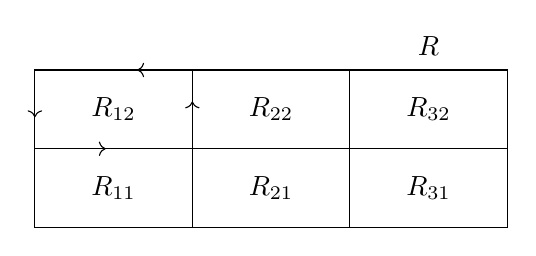
\begin{tikzpicture}
\draw (0,0) rectangle (6,2);
\draw (0,1) -- (6,1);
\draw (2,0) -- (2,2);
\draw (4,0) -- (4,2);
\node at (5,2.3) {$R$};
\node at (1,1.5) {$R_{12}$};
\node at (3,1.5) {$R_{22}$};
\node at (5,1.5) {$R_{32}$};
\node at (1,0.5) {$R_{11}$};
\node at (3,0.5) {$R_{21}$};
\node at (5,0.5) {$R_{31}$};
\draw[->] (1.7,2) -- (1.3,2);
\draw[->] (0,1.8) -- (0,1.4);
\draw[->] (0.4,1) -- (0.9,1);
\draw[->] (2,1.2) -- (2,1.6);
\end{tikzpicture}\end{diagramblock}

\uline{Exercice :} (de topologie)
justifier en détail le fait que $R$ peut être décomposer en rectangles
$R_{i,j} = A_i \times B_j$ contenu chacun dans un ouvert du sous-recouvrement fini obtenu.

\margin{168}

\clearpage
% Cote 119: offprints, reports, courses, CV and letters (typed and printed part): archive cote 119, site page 169 (PDF page 170).
% typescript. Draft compared: none.
% AI-transcribed by Claude Opus 5.5 (claude-opus-5-5, adaptive thinking, effort high), Message Batches API, batch r119_full (msgbatch_01DwZNm5Y7YsKBWyAN4sFs8w), 2026-11-13; not yet checked by eye.
\scanpage{119/169}
\mspage{- 8 -}

4. \uline{Fonctions holomorphes}

Les fonctions dérivables rencontrés en 4.5. p;19 du fascicule
SERIES ENTIERES vont porter désormais le nom plus glorieux de fonctions
holomorphes et le but annoncé dans l'introduction est de montrer que les
fonctions holomorphes sont analytiques ce qui justifiera a posteriori la
terminologie signalée dans le fascicule FONCTIONS ANALYTIQUES p. 3 .
Par abus de notation on notera souvent par la même lettre $f$ une fonction
d'un ouvert $U$ du plan complexe dans le plan complexe et la fonction induite
en ``oubliant'' la structure complexe de U. Soit $Z = X+iY$ . On écrira :
$f(Z) = f(X,Y)$. On désignera de même par $U$ l'ouvert de $R^{2}$ image de $U$ par
l'application canonique $x+iy \rightarrow (x,y)$ .

\uline{Définition 4.1.}

On dit que $f$ est $\mathbb{R}$-différentiable au point $(x_{o},y_{o}) \in U$ s'il
existe une fonction linéaire $(h,k) \rightarrow ak + bk$ de $R^{2}$ dans $\mathbb{C}$ telle que l'on
ait la relation :
\[ (4.1) \quad f(x_{o}+h,\ y_{o}+k) - f(x_{o},y_{o}) = ah + bk + o(\sqrt{h^{2}+k^{2}}) \quad (\text{où } O\ (\sqrt{h^{2}+k^{2}}) \]
désigne un infiniment petit par rapport à $\sqrt{h^{2}+k^{2}}$) . Si $f$ est $\mathbb{R}$-diffé-%
rentiable au point $(x_{o},y_{o})$ les constantes $a$ et $b$ sont déterminées de manière
unique et on a :
\[ a = \frac{\partial f}{\partial x}\,(x_{o},y_{o}) \qquad b = \frac{\partial f}{\partial y}\,(x_{o},y_{o}) \]
Rappelons que l'existence des dérivées partielles au point $(x_{o},y_{o})$ n'est pas
suffisante pour que la fonction soit dérivable en ce point. Mais on \inserted[typed]{a} la ``réci-%
proque'' suivante :
Si $f$ possède des dérivées partielles dans un voisin\unsure{a}ge de $(x_{o},y_{o})$ et si ces
dérivées partielles sont continues au point $(x_{o},y_{o})$ alors $f$ est différentia-%
ble en ce point.

\margin{169}

\clearpage
% Cote 119: offprints, reports, courses, CV and letters (typed and printed part): archive cote 119, site page 170 (PDF page 171).
% typescript. Draft compared: none.
% AI-transcribed by Claude Opus 5.5 (claude-opus-5-5, adaptive thinking, effort high), Message Batches API, batch pilotnext (msgbatch_01A9sdu8SYq23bEtqX9tUncQ), 2026-11-13; not yet checked by eye.
\scanpage{119/170}
\mspage{- 9 -}

Si cela est le cas dans tout l'ouvert  $U$  on dit que  $f$  est \unsure{continûment}
différentiable dans  $U$.

\uline{Définition 4.2.}  (identique à 4.5 de Séries  Entières)

On dit que  $f$  est holomorphe au point  $z_o \in U$  si
\[ \lim_{\substack{u\to 0\\ u\neq 0}} \ (f(Z_o+u) - f(Z_o))/u \ \text{ existe} \]

En notant  $f'(z_o)$  cette limite, on a donc :  $f(Z_o+u)-f(Z_o) = f'(Z_o).u + O(|u|$\unsure{$^\circ$}

En posant  \unsure{$(u =)h + ik$|$u = h + ik$}  on a en comparant avec la relation  (4.1)  le fait
que  $f$  est $\mathbb{R}$-différentiable avec de plus  $a = f'(Z_o)$ et $b = i\, f'(Z_o)$
d'où en remplaçant  $a$ et $b$  par leur valeurs :
\[ \frac{\partial f}{\partial y} = i\,\frac{\partial f}{\partial x} \quad \text{ou encore} \quad \frac{\partial f}{\partial x} + i\,\frac{\partial f}{\partial y} = 0 \ . \]

Réciproquement si  $f$  est  $R$-différentiable et vérifie la relation précédente,
(4.1) montre que  $f$  est holomorphe en  $Z_o$. Si  $f = P + iQ$, les fonctions
$P$ et $Q$  étant réelles on obtient les conditions de Cauchy :
\[ \frac{\partial P}{\partial x} = \frac{\partial Q}{\partial y} \ , \quad \frac{\partial P}{\partial y} = -\frac{\partial Q}{\partial x} \]

\uline{4.3. Théorème de Cauchy}

Si  $f(Z)$  est holomorphe dans un ouvert  $U$  du plan complexe, la
forme différentielle  $f(Z)\, dZ$  est fermée dans  $U$.

\uline{Démonstration :}

D'après la proposition 3.6. il nous suffit de prouver que
$\int_\gamma f(Z)\, dZ = 0$  chaque fois que  $\gamma$  est le bord d'un rectangle contenu (ainsi
que son intérieur) dans  $U$  et ayant ses côtés parallèles aux axes. Soit  $R$
un tel rectangle. Posons a priori  $\int_\gamma f(Z)\, dZ = \alpha(R)$ . Partageons le rectan-%
gle  $R$  en quatre rectangles égaux en partageant chacun de ses côtés en
deux parties égales. Soit  $\gamma_i$  les bords orientés des rectangles obtenus

\mspage{\hand{170}}

\clearpage
% Cote 119: offprints, reports, courses, CV and letters (typed and printed part): archive cote 119, site page 171 (PDF page 172).
% typescript. Draft compared: none.
% AI-transcribed by Claude Opus 5.5 (claude-opus-5-5, adaptive thinking, effort high), Message Batches API, batch r119_full (msgbatch_01DwZNm5Y7YsKBWyAN4sFs8w), 2026-11-13; not yet checked by eye.
\scanpage{119/171}
\mspage{- 10 -}

$R_1$, $R_2$, $R_3$, $R_4$. On vérifie (comme en 3.4) que
\[ \alpha(R) = \int_\gamma f(Z)\, dZ = \sum_{i=1}^{4} \int_{\gamma_i} f(Z)\, dZ = \sum_{i=1}^{4} \alpha(R_i) \]
Donc parmi ces quatre rectangles il y en a au moins un tel que
$|\alpha(R_i)| \geq \frac{1}{4}\, |\alpha(R)|$ . Appelons $R^{(1)}$ ce \unsure{rectangme|rectangle}.
En réitérant l'opération précédente sur le rectangle $R^{(1)}$ on trouve un
rectangle $R^{(2)}$ tel que $|\alpha(R^{(2)})| \geq \frac{1}{4}\, |\alpha(R^{(1)}| \geq \frac{1}{4^2}\, |\alpha(R)|$.
On peut recommencer indéfiniment la même opération. On obtiendra ainsi une suite
de rectangles emboités ; le k-ième aura ses côtés $2^k$ fois plus petit que ceux
de $R$ et son aire sere $4^k$ fois plus petite que celle de $R$.
Si $\gamma(k)$ désigne le bord orienté du rectangle $R^{(k)}$ on a :
\[ \text{(4.3.1.)} \qquad \Big|\int_{\gamma(k)} f(Z)\, dZ\Big| \geq \frac{1}{4^k}\, \alpha(R) \ . \]
L'intersection des rectangles $R^{(k)}$ est égale à un point $Z_0$
(justifiez). On a $Z_0 \in U$ . Comme $f$ est holomorphe en $Z_0$. On a :
\[ f(Z) = f(Z_0) + f'(Z_0)\ (Z-Z_0) + \epsilon(Z)\, |Z-Z_0| \quad \text{avec} \ \lim_{Z \to Z_0} \epsilon(Z) = 0 \]
on en désuit :
\[ \int_{\gamma(k)} f(Z)\, dZ = f(Z_o) \int_{\gamma(k)} dZ + f'(Z_0) \int_{\gamma(k)} (Z-Z_0)\, \unsure{dZ} + \int_{\gamma(k)} \epsilon(Z)\, |Z-Z_0|\, dZ \]
les deux premières intégrales sont nulles (proposition 3.3). Si $a$ et $b$ désignent
les longueurs des côtés du rectangle $R$ avec $a \geq b$. On a :
\[ |Z-Z_0| \leq \sqrt{a^2+b^2}\ .\ 2^{-k} \]
périmètre de $R^{(k)} = 2(a+b).2^{-k}$ d'iù si $k$ est assez grand pour que $|\epsilon(Z)| \leq \epsilon$
quelque soit $Z$ sur la frontière de $R^{(k)}$ :
(4.3.2)
\[ \Big|\int_{\gamma(k)} \epsilon(Z)\, |Z-Z_0|\, dZ\Big| \leq \epsilon\ .\ K\ .\ 4^{-k} \quad \text{où $K$ est une constante positive.} \]
On a donc en comparant (4.3.1) et (4.3.2) :
$\alpha(R) \leq \epsilon.K$ et ce, pour tout,$\epsilon > 0$, ce qui montre que $\alpha(R) = 0$ et
achève la démonstration.

\margin{171}

\clearpage
% Cote 119: offprints, reports, courses, CV and letters (typed and printed part): archive cote 119, site page 172 (PDF page 173).
% typescript. Draft compared: none.
% AI-transcribed by Claude Opus 5.5 (claude-opus-5-5, adaptive thinking, effort high), Message Batches API, batch r119_full (msgbatch_01DwZNm5Y7YsKBWyAN4sFs8w), 2026-11-13; not yet checked by eye.
\scanpage{119/172}
\mspage{- 11 -}

\uline{Théorème 4.4}.

Si $f(Z)$ est continue dans un ouvert $U$ du plan complexe et holo-%
morphe en tout point de $U$ sauf éventuellement en des points isolés la forme
$f(Z)\ dZ$ est fermée.

\uline{Démonstration}. D'après le théorème de Bolzano-Weier\unsure{strass} si $R$ est un
rectangle contenu dans $U$ il ne peut y avoir qu'un nombre fini de points de
$R$ où $f$ n'est pas holomorphe. En utilisant un découpage de $R$ par des paral-%
lèles aux axes passant par ces points (découpage analogue à celui rencontré
dans 3.6.) on est amené à démontrer que $\int_{\gamma} f(Z)\ dZ = 0$ dans le cas où $\gamma$
est un rectangle contenant au plus un sommet où $f$ n'est pas holomorphe. Soit
$(x_0,y_0)$ un tel sommet, $(x_0+a,\ y_0)$, $(x_0,y_0+b)$, $(x_0+a,\ y_0+b)$ les autres sommets
du rectangle. Supposons par exemple $a > 0$, $b > 0$. D'après 4.3. l'intégrale
de $f(Z)\ dZ$ le long de $\gamma_{\varepsilon}$ bord du rectangle $(x_0,y_0+\varepsilon)$ , $(x_0+a,y_0+\varepsilon)$ ,
$(x_0+a,y_0+b)$, $(x_0,\ y_0+b)$ est nulle et du fait de la continuité de $f$ cette
intégrale, tend vers $\int_{\gamma} f(Z)\ dZ$ quand $\varepsilon$ tend vers 0. Ce qui nous donne le
résultat attendu.

5 . \uline{Développement en série entière d'une fonction holomorphe}

\uline{Définition 5.1}.

Etant donnés un chemin différentiable fermé $\gamma$ dans le plan $C$ et
$Z_0$ un point de $C$ n'appartenant pas à l'image de $\gamma$ on appelle indice de $\gamma$
par rapport à $Z_0$ et on note $I(\gamma,Z_0)$ la valeur de l'intégrale
\[ \frac{1}{2\Pi i} \int_{\gamma} \frac{dZ}{Z-Z_0} \]

\uline{Proposition 5.2.}

$I(\gamma,Z)$ est un entier constant quend $Z$ vraie dans une composante
connexe du complémentaire de l'image de $\gamma$. Pour $Z$ dans la composante non
bornée de ce complémentaire on a $I(\gamma,Z) = 0$ .

\margin{172}

\clearpage
% Cote 119: offprints, reports, courses, CV and letters (typed and printed part): archive cote 119, site page 173 (PDF page 174).
% typescript. Draft compared: none.
% AI-transcribed by Claude Opus 5.5 (claude-opus-5-5, adaptive thinking, effort high), Message Batches API, batch r119_full (msgbatch_01DwZNm5Y7YsKBWyAN4sFs8w), 2026-11-13; not yet checked by eye.
\scanpage{119/173}
\mspage{- 12 -}

\uline{Démonstration}. Soit $[a,b]$ le domaine de définition de $\gamma$.

(5.2.1.) Alors $(\gamma,Z) = \dfrac{1}{2\Pi i}\displaystyle\int_a^b \dfrac{\gamma'(t)\,dt}{\gamma(t) - Z}$

Comme $w/2\Pi i$ est entier si et seulement si $e^{w} = 1$, il s'agit de montrer que

$\varphi(b) = 1$ où $\varphi$ est défini par
\[ \varphi(s) = \exp \{ \int_a^s \frac{\gamma'(t)}{\gamma(t)-Z}\,dt\} \quad \text{pour } a \leq s \leq b \text{ .} \]
soit en dérivant les deux membres.
\[ \frac{\varphi'(s)}{\varphi\ (s)} = \frac{\gamma'(s)}{\gamma(s)-Z} \quad \text{sauf éventuellement aux points (en nombre fini) où} \]
$\gamma$ n'est pas différentiable.

Par conséquent $\dfrac{\varphi}{\gamma-Z}$ est une fonction continue sur $[a,b]$ dont la dérivée est
nulle sur $[a,b]$ (moins éventuellement un nombre fini de points). Donc $\dfrac{\varphi}{\gamma-Z}$
est constante sur $[a,b]$ et comme $\varphi(a) = 1$ on obtient
\[ \frac{\varphi(s)}{\gamma(s) - Z} = \frac{1}{\gamma(a) - Z} \]
comme de plus $\gamma(a) = \gamma(b)$ pour $s = b$ on obtient $\varphi(b) = 1$ ce qui montre
que $I(\gamma,Z)$ est un entier.

Comme $[a,b]$ est compact et $\gamma$ continue l'image de $\gamma$ est compacte
donc contenue dans un disque compact dont le complémentaire est connexe ce
qui montre que le complémentaire de l'image de $\gamma$ a exactement une composante
non bornée.

(5.2.1) montre que pour $|Z|$ assez grand on a $|I(\gamma,Z)| < 1$ et comme
l'indice est entier la proposition est prouvée.

\uline{5.3. Exemple}.

Si $\gamma$ est le cercle orienté dans le sens direct de centre $Z_0$ et
de rayon $r$ on a :
\[ I(\gamma,Z) = 0 \ \text{si}\ |Z - Z_0| > r \]
\[ I(\gamma,Z) = 1 \ \text{si}\ |Z - Z_0| < r \ . \]

\margin{173}

\clearpage
% Cote 119: offprints, reports, courses, CV and letters (typed and printed part): archive cote 119, site page 174 (PDF page 175).
% typescript. Draft compared: none.
% AI-transcribed by Claude Opus 5.5 (claude-opus-5-5, adaptive thinking, effort high), Message Batches API, batch r119_full (msgbatch_01DwZNm5Y7YsKBWyAN4sFs8w), 2026-11-13; not yet checked by eye.
\scanpage{119/174}
\mspage{- 13 -}

Pour cela il ne reste à prouver que $I(\gamma, Z_0) = 1$ ce qui résulte de
\[ \int_{\gamma} \frac{dZ}{Z - Z_0} = \int_0^{2\Pi} \frac{ri\; e^{i\theta}}{r\; e^{i\theta}}\, d\theta = 2\,\Pi i \]
La proposition 3.3 nous montre que si $\dfrac{dZ}{Z - Z_0}$ est une forme différentielle
fermée sur $C - \{Z_0\}$ elle n'a pourtant pas de primitive sur cet ouvert.

\uline{5.4. Proposition}.

Soit $f$ une fonction holomorphe dans un ouvert $U$ de $C$, $Z_0 \in U$ ,
$r > 0$ tel que le disque fermé $\bar{B}(Z_0, r)$ soit contenu dans $U$\unsure{,} et $\gamma$ le bord
de ce disque parcouru dans le sens direct. On a alors pour $|Z_1 - Z_0| < r$
\[ (5.4.1.) \qquad \frac{1}{2\,\Pi i} \int_{\gamma} \frac{f(Z)\, dZ}{Z - Z_1} = f(Z_1) \]
\uline{Démonstration}.

Soit $g(Z)$ la fonction définie dans $U$ par
\[ g(Z) = \frac{f(Z) - f(Z_{\over{0}{1}})}{Z - Z_{\over{0}{1}}} \qquad \text{pour } Z \neq Z_0 \]
\[ g(Z) = f'(Z_{\over{0}{1}}) \qquad \text{pour } Z = Z_0 \]

La fonction $g$ est continue sur $U$ par définition de la dérivée.
Elle est holomorphe en tout point de $U$ autre que le point $Z$. D'après le
théorème 4.4. la forme $g(Z)\, dZ$ est fermée dans $U$. Si $r' > r$ est tel que
le disque $B(Z_0, r')$ est contenu dans $U$ (un tel $r'$existe. pourquoi ?)
$g(Z)\, dZ$ est fermée dans $B(Z_0, r')$ et donc d'après les propositions (3.4)
et (3.6) a une primitive dans $B(Z_0, r')$ et on a alors (proposition 3.3.)
$\int_{\gamma} g(Z)\, dZ = 0$ d'où le résultat d'après (5.3.) .

\uline{5.5. Théorème}

Soit $f(Z)$ une fonction holomorphe dans un disque ouvert $|Z - Z_0| < \rho$ ;
alors $f$ est développable en série entière dans ce disque.

\margin{174}

\clearpage
% Cote 119: offprints, reports, courses, CV and letters (typed and printed part): archive cote 119, site page 175 (PDF page 176).
% typescript. Draft compared: none.
% AI-transcribed by Claude Opus 5.5 (claude-opus-5-5, adaptive thinking, effort high), Message Batches API, batch r119_full (msgbatch_01DwZNm5Y7YsKBWyAN4sFs8w), 2026-11-13; not yet checked by eye.
\scanpage{119/175}
\mspage{- 14 -}

\uline{Démonstration .}

Soit \( r < \rho \). On va trouver une série entière qui converge normale-%
ment vers \( f(Z) \) pour \( |Z| \leq r \) . Cette série sera indépendante de \( r \) en vertu
de l'unicité du développement en série entière d'une fonction au voisinage de
\( Z_0 \). Le théorème en résultera donc.

Choisissons \( r_0 \) tel que \( r < r_0 < \rho \) . Appliquons le théorème 5.4.
en prenant pour \( \gamma \) le cercle de centre \( Z_0 \) et de rayon \( r_0 \). Pour \( |Z-Z_0| \leq r \)
on a : \( f(Z) = \frac{1}{2 \pi i} \int_{\gamma} \frac{f(t)\, dt}{t - Z} \)
Comme \( |Z-Z_0| < |t-Z_0| \) on peut développer \( \frac{1}{t - Z} \) :
\[ \frac{1}{t - Z} = \frac{1}{t - Z_0} \;.\; \frac{1}{1 - \frac{Z-Z_0}{t-Z_0}} = \frac{1}{t - Z_0} \Bigl( 1 + \frac{Z - Z_0}{t - Z_0} + \Bigl( \frac{Z - Z_0}{t - Z_0} \Bigr)^2 + \dots \Bigr) \]

On a donc :
\[ f(Z) = \frac{1}{2 \pi \, i} \int_{\gamma} \sum_{n \geq 0} \frac{(Z-Z_0)^n}{(t-Z_0)^{n+1}} f(t)\, dt \]

La série converge normalement pour \( |Z - Z_0| \leq r \) et \( |t - Z_0| = r_0 \) on
peut donc l'intégrer terme à terme et on obtient une série normalement conver-%
gente pour \( |Z - Z_0| \leq r \) . (Rappeler la justification de ce fait constitue
un bon exercice).

On obtient donc :
\[ (5.5.1.) \qquad f(Z) = \sum_{n \geq 0} a_n \, (Z - Z_0)^n \]
où les coefficients \( a_n \) sont donnés par les intégrales
\[ (5.5.2.) \qquad a_n = \frac{1}{2 \pi i} \int_{|t-Z_0| = r_0} \frac{f(t)\, dt}{(t-Z_0)^{n+1}} \]

Le théorème est donc démontré.

(5.6.) \uline{Remarque.}

On a obtenu plus que le résultat attendu puisque non seulement on
a prouvé que toute fonction holomorphe est analytique mais on a montré de plus

\margin{175}

\clearpage
% Cote 119: offprints, reports, courses, CV and letters (typed and printed part): archive cote 119, site page 176 (PDF page 177).
% typescript. Draft compared: none.
% AI-transcribed by Claude Opus 5.5 (claude-opus-5-5, adaptive thinking, effort high), Message Batches API, batch r119_full (msgbatch_01DwZNm5Y7YsKBWyAN4sFs8w), 2026-11-13; not yet checked by eye.
\scanpage{119/176}
\mspage{- 15 -}

que le développement en série entière autour d'un point $Z_0$ du domaine $U$
de $f$ était valable dans le plus grand disque ouvert de centre $Z_0$ contenu
dans $U$ ce qui n'était pas évident à partir de la définition des fonctions
analytiques.

(5.7.) \uline{Théorème de Morera} (réciproque de 4.3.)

Soit $f$ une fonction continue dans \unsure{uncouvert|un ouvert} $U$ du plan. Si la forme
différentielle $f(Z)\,dZ$ est fermée alors $f$ est holomorphe dans $D$.

En effet $f$ admet localement une primitive $g$. Cette primitive est
holomorphe (elle a une dérivée $f$) et d'après (5.5.) $g$ est analytique donc
$f$ est aussi analytique C.Q.F.D.

En particulier si $f$ est continue dans $U$ et holomorphe en tout point de $U$
sauf éventuellement en des points isolés $f$ est holomorphe dans $U$ tout
entier card'après (4.4.) $f(Z)\,dZ$ est fermée et (5.7.) nous donne la
conclusion.

6 . \uline{Homotopie de chemins}

Une conséquence des propositions 3.4. et 3.6. est que les disques
ouverts du plan possèdent la propriété suivante :

6.1. Toute forme différentielle fermée sur un disque ouvert admet une
primitive sur ce disque ouvert.

On va voir que l\unsure{e}s disque sont loin d'être les seuls ouverts à posséder cette
propriété. En fait les ouverts possédant cette propriété sont les ouverts
``simplement connexe'' c'est-à-dire ceux qui n'ont pas de ``trous''. Nous allons
préciser cette notion vague en donnant un sens clair à la notion de chemin qui
se déforme continûment.

Pour simplifier on ne va considérer que des chemins paramétrés par le segment
$I = \hand{[}0,1\hand{]}$ . (on pourra de toutes façons se ramener à ce cas par un changement
de paramètre).

\margin{176}

\clearpage
% Cote 119: offprints, reports, courses, CV and letters (typed and printed part): archive cote 119, site page 177 (PDF page 178).
% typescript. Draft compared: none.
% AI-transcribed by Claude Opus 5.5 (claude-opus-5-5, adaptive thinking, effort high), Message Batches API, batch r119_full (msgbatch_01DwZNm5Y7YsKBWyAN4sFs8w), 2026-11-13; not yet checked by eye.
\scanpage{119/177}
\mspage{- 16 -}

6.2. \uline{Définition}.

On dit que deux chemins
\[ \gamma_0 : I \to U \quad \text{et} \quad \gamma_1 : I \to U \qquad \text{(U ouvert)} \]
sont homotopes dans U s'il existe une application continue
\[ \delta : I \times I \to U \qquad (t,u) \to \delta(t,u) \]
telle que \qquad $\delta(t,0) = \gamma_0(t)$

(6.2.1)

\qquad\qquad $\delta(t,1) = \gamma_1(t)$

Si $\gamma_0$ et $\gamma_1$ ont même origine et même extrémité on dit que $\gamma_1$ et $\gamma_1$
sont homotopes avec extrémités fixes

(6.2.2.) \qquad si de plus : \qquad $\delta(0,u) = \gamma_0(0) = \gamma_1(0)$

\qquad\qquad $\delta(1,u) = \gamma_0(1) = \gamma_1(1)$

Si $\gamma_0$ et $\gamma_1$ sont des chemins fermés\unsure{,} on dit qu'ils sont homotopes comme
chemins fermés si l'homotopie $\delta$ vérifie.
\[ \delta(t,0) = \gamma_0(t) \]
(6.2.1.)
\[ \delta(t,1) = \gamma_1(t) \]

(6.2.3.) \qquad $\delta(0,u) = \delta(\unsure{1},u)$

autrement dit s'ils sont homotopes et si pour tout u : $t \to \delta(t,u)$ est un
chemin fermé. (Si $\gamma_1(t)$ est constante on dira que le chemin fermé $\gamma_0(t)$
est homotope à un point).

6.3. \uline{Définition}.

Un ouvert U est simplement connexe si tout chemin fermé dans U
est homotope à un point (comme chemin fermé bien sûr).et si U est connexe.

6.4. \uline{Exemples} : Un disque est simplement connexe. Un ensemble convexe et plus
généralement un ensemble étoilé est simplement connexe. (Un ensemble U est
étoilé par rapport à $Z_0 \in U$ siopour tout $Z \in U$ le segment $[Z_0,Z]$ est
contenu dans U). Il suffit de considérer l'homotopie
\[ \delta(t,u) = u\,(\gamma(t) - Z_0) + Z_0 \ . \]
Le plan complexe privé des points réels négatifs est donc simplement connexe.
C - \{0\} ne l'est pas. Une couronne n'est pas simplement connexe.

\mspage{177}

\clearpage
% Cote 119: offprints, reports, courses, CV and letters (typed and printed part): archive cote 119, site page 178 (PDF page 179).
% typescript. Draft compared: none.
% AI-transcribed by Claude Opus 5.5 (claude-opus-5-5, adaptive thinking, effort high), Message Batches API, batch r119_full (msgbatch_01DwZNm5Y7YsKBWyAN4sFs8w), 2026-11-13; not yet checked by eye.
\scanpage{119/178}
\mspage{- 17 -}

6.5. \uline{Théorème}.

Soit $(t,u) \to \delta(t,u)$ une application continue d'un rectangle
$a \leq t \leq b$ , $a' \leq u \leq b'$ dans l'ouvert $U$ et soit $\omega$ une forme différen-%
tielle fermée dans $U$. Alors il existe une application $f(t;u)$ continue dans
le rectangle telle que au voisinage de tout point $(t_0,u_0)$ du rectangle
il existe une primitive $F$ de $\omega$ vérifiant $F(\delta(t;u)) = f(t,u\unsure{)|=}$ .
(Une telle fonction $f$ sera appelée primitive de $\omega$ suivant l'application $\delta$).
Cette primitive est unique à l'addition d'une constante près.

\uline{Démonstration}. Il s'agit encore d'une démonstration facile mais technique
basée sur la compacité du rectangle. En utilisant celle-ci on obtient des
subdivisions de $[a,b]$ et $[a',b']$
\[ a = t_0 < t_1 < t_2 \ \dots < t_n = b \]
\[ a' = u_0 < u_1 < u_2 \ \dots < u_m = b' \]
telles que le produit $[t_i, t_{i+1}] \times [u_j, u_{j+1}]$ soit un rectangle appliqué
par $\delta$ dans un disque ouvert $U_{i,j}$ dans lequel existe une primitive $F_{i,j}$
de $\omega$ . Fixons $j$. Comme $U_{i,j} \cap U_{\unsure{ix1|i\times 1},j}$ est non vide et connexe on peut
ajouter à chaque $F_{i,j}$ ($i$ variable) une constante telle que $F_{i,j}$ et
$F_{i+1,j}$ coïncident dans $U_{i,j} \cap U_{i+1, j}$ (remarque suivant la définition 3.2)
On obtient alors pour $u \in [u_j, u_{j+1}]$ une fonction $f_j(t,u)$ telle que
pour tout $i$ on ait
\[ f_j(t,u= = F_{i,j} \ (\delta(t,u)) \ \text{lorsque} \ t \in [t_i, t_{i+1}] \]
Ainsi $f_j(t,u)$ est continue dans le rectangle
\[ a \leq t \leq b \qquad u_j \leq u \leq u_{j+1} \]
Soit $V_j = \bigcup_{i=0}^{n} U_{i,j}$
$V_j \cap V_{i,j+1}$ est non vide et connexe car pour tout $i$ . $U_{i,j} \cap U_{i,j+1}$ est
connexe et contient $\delta([t_i,t_{i+1}] \times \{u_{j+1}\})$ . $[\delta([a,b] \times \{u_{j+1}\}$ est connexe.

\margin{178}

\clearpage
% Cote 119: offprints, reports, courses, CV and letters (typed and printed part): archive cote 119, site page 179 (PDF page 180).
% typescript. Draft compared: none.
% AI-transcribed by Claude Opus 5.5 (claude-opus-5-5, adaptive thinking, effort high), Message Batches API, batch r119_full (msgbatch_01DwZNm5Y7YsKBWyAN4sFs8w), 2026-11-13; not yet checked by eye.
\scanpage{119/179}
\mspage{- 18 -}

On se reportera avec profit à la feuille d'exercices n\textsuperscript{o} 4. II 2\textsuperscript{o} b \unsure{(}et 3\textsuperscript{o} a).

On peut donc en ajoutant des constantes aux $f_j$ (c'est-à-dire en
modifiant une fois de plus les $F_{i,j}$ choisis) rendre $f_j(t,u)$ et $f_{j+1}(t,u)$
égales pour $u = u_{j+1}$. La fonction $f(t,u)$ définie par $f(t,u) = f_j(t,u)$
pour $u \in [u_j, u_{j+1}]$ est bien continue et vérifie $F_{i,j}(\delta(t,u)) = f(t,u)$
pour $t_i \leq t \leq t_{i+1}$, $u_j \leq u \leq u_{j+1}$ ce qui démontre l'existence de f.
Si $f_1$ et $f_2$ sont deux telles fonctions, au voisinage de tout point $(t_0,u_0)$
du rectangle $[a,b] \times [a',b']$ on a
$f_1(t,u) - f_2(t,u) = F_1(\delta(t,u)) - F_2(\delta(t,u))$ qui est constant. La
fonction $f_1-f_2$ \unsure{est} donc ``localement\unsure{''} constante''. Comme le rectangle
$[a,b] \times [a',b']$ est connexe on voit facilement que $f_1-f_2$ est constante
d'où la dernière assertion.

Le cas où pour chaque $t$ la fonction $u \to \delta(t,u)$ est constante nous
fournit le résultat intéressant :

6.6. \uline{Corollaire}

Soit $\gamma : [a,b \to U$ un \unsure{clemin|chemin} contenu dans l'ouvert U ($\gamma$ est une
application continue) et soit $\omega$ une forme différentielle fermée dans U. Il
existe une fonction f continue sur $[a,b]$ telle que au voisinage de tout
point $\gamma\ (t_0)$ ($a \leq t_0 \leq b$) il existe une primitive F de $\omega$ telle que
$F(\gamma(t)) = f(t)$ . f est unique à l'addition d'une constante près.
(On dira que f est une primitive de $\omega$ le long de $\gamma$).

6.7. \uline{Remarque}.

Si $\gamma$ est différentiable par morceaux, f une primitive de $\omega$
suivant $\gamma$ on vérifie facilement que $\int_\gamma \omega = f(b) - f(a)$.
D'après (6.6) cette formule donne une définition de $\int_\gamma \omega$ dans le cas où $\gamma$

\margin{179}

\clearpage
% Cote 119: offprints, reports, courses, CV and letters (typed and printed part): archive cote 119, site page 180 (PDF page 181).
% typescript. Draft compared: none.
% AI-transcribed by Claude Opus 5.5 (claude-opus-5-5, adaptive thinking, effort high), Message Batches API, batch r119_full (msgbatch_01DwZNm5Y7YsKBWyAN4sFs8w), 2026-11-13; not yet checked by eye.
\scanpage{119/180}
\mspage{- 19 -}

est un chemin continu non nécessairement différentiable par morceaux.

6.8. \uline{Théorème}.

Si $\gamma_0$ et $\gamma_1$ sont deux chemins fermés dans U, homotopes comme
chemins fermés on a $\int_{\gamma_0} \omega = \int_{\gamma_1} \omega$ pour toute forme fermée $\omega$ dans U.

\uline{Démonstration} :

Soit $\delta$ vérifiant (\unsure{6}.2.1) et (6.2.3.) .

Soit f une primitive de $\omega$ suivant $\delta$. (théorème 6.5.). Pour u fixé
$t \to f(t,u)$ est une primitive de $\omega$ suivant $t \to \delta(t,u)$. On a donc (6.7)
$\int_{\gamma_0} \omega = f(1\unsure{,}0) - f(0,0)$
$\int_{\gamma_1} \omega = f(1,1) - f(0,1)$
Comme d'après (6.2.3) on a : $\delta(0,u) = \delta(1,u)$, $f(0,u)$ et $f(1,u)$ primitives
de $\omega$ suivant le chemin $u \to \delta(0,u)$ diffèrent d'une constante. En particulier
$f(1,1) - f(0,1) = f(1,0) - f(0,0)$ C.Q.F.D.

6.9. \uline{Corollaire}.

Toute forme différentielle fermée $\omega$ dans un ouvert simplement con-%
nexe U possède une primitive dans U.

\uline{Démonstration}.

D'après \unsure{(6,8)|(6.8)} on a $\int_{\gamma} \omega = 0$ pour tout chemin fermé $\gamma$. Car un
tel c hemin est homotope à un point. On conclut grâce à (3.3) .

\margin{180}

\clearpage
% Cote 119: offprints, reports, courses, CV and letters (typed and printed part): archive cote 119, site page 182 (PDF page 183).
% typescript. Draft compared: none.
% AI-transcribed by Claude Opus 5.5 (claude-opus-5-5, adaptive thinking, effort high), Message Batches API, batch r119_full (msgbatch_01DwZNm5Y7YsKBWyAN4sFs8w), 2026-11-13; not yet checked by eye.
\scanpage{119/182}
UNIVERSITE DES SCIENCES \& TECHNIQUES \qquad ANNEE UNIVERSITAIRE 1973-74

DU LANGUEDOC

Mathématiques

M. P. II

FONCTIONS HOLOMORPHES

\uline{(Suite et fin)}

6.10. \uline{Corollaire}

Si $f(z)$ est holomorphe dans $U$, on a $\int_{\gamma} f(z)\,dz = 0$ pour tout che-%
min fermé $\gamma$ de $U$ qui est homotope à un point dans $U$.

\uline{Démonstration} : la forme $f(x)\,dz$ est fermée (théorème de Cauchy 4.3). On ap-%
plique 6.8.

On peut donner aussi une forme plus générale de la proposition 5.4.

6.1.1. \uline{Proposition}.

Soit \unsure{$f$} une fonction holomorphe dans un ouvert $U$. Soit $a \in U$ et
soit $\gamma$ un chemin fermé de $U$ ne passant pas par $a$ et homotope à un point
dans $U$. On a alors
\[ (6.11.1) \qquad \frac{1}{2\,\pi\, i}\int_{\gamma} \frac{f(z)\,dz}{z-a} = I(\gamma,a)\ \ f(a) \]
où $I(\gamma,a)$ est défini en (5.1).

\uline{Démonstration} :la démonstration est identique à celle de (5.4) $g(z)$ étant dé-%
fini par $\dfrac{f(z) - f(a)}{z-a}$ si $z \neq a$ et par $g(a) = f'(a)$ le théorème 4.4 montre
que $g(z)\,dz$ est fermée et le théorème 6.8. montre que $\int_{\gamma} g(z)\,dz = 0$ d'où
le résultat par définition de l'indice.

7. \uline{Principe du maximum}

(7.1.) \uline{Inégalités de Cauchy}

Soit $f$ une fonction holomorphe dans la boule ouverte $B(z_o,\rho)$ et
$r$ un nombre tel que $0 < r < \rho$. On a vu dans (5.5) que pour $|z - z_o| < \rho$ on
a:

\mspage{\hand{182}}

\clearpage
% Cote 119: offprints, reports, courses, CV and letters (typed and printed part): archive cote 119, site page 183 (PDF page 184).
% typescript. Draft compared: none.
% AI-transcribed by Claude Opus 5.5 (claude-opus-5-5, adaptive thinking, effort high), Message Batches API, batch r119_full (msgbatch_01DwZNm5Y7YsKBWyAN4sFs8w), 2026-11-13; not yet checked by eye.
\scanpage{119/183}
\mspage{- 2 -}

(5.5.1) \quad $f(z) = \sum_{n \geq 0} a_n \, (z-z_o)^n$ \quad où les coefficients sont donnés par
\[ a_n = \frac{1}{2 \pi i} \int_{|t-z_o|=r} \frac{f(t)}{(t-z_o)^{n+1}} \, dt \]
Faisons le changement de variable \quad $(t-z_o) = r e^{i\theta}$
\[ (7.1.1) \qquad a_n r^n = \frac{1}{2\pi} \int_0^{2\pi} e^{-n^{i\theta}} \, f(z_o + re^{i\theta}) \, d\theta \]

formule que l'on obtiendrait tout aussi bien à partir de
\[ f(z_o + re^{i\theta}) = \sum_{p \geq 0} a_p r^n e^{pi\theta} \]
en multipliant par $e^{-ni\theta}$ et en intégrant sur $[0,2\pi]$ car pour $r$ fixé la série
précédente est normalement \unsure{convergente}.

Si nous posons
\[ (7.1.2) \qquad M_{z_o}(r) = \sup_{0 \leq \theta \leq 2\pi} |f(z_o + re^{i\theta})| \quad \text{on obtient l'inégalité} \]
\[ (7.1.3) \qquad |a_n| \leq \frac{M_{z_o}(r)}{r^n} \quad \text{en majorant (7.1.1)} \]

Ce sont les \uline{inégalités de Cauchy}. On savait déjà (Séries Entières
début) que, comme $r < \rho$, $|a_n| r^n$ était majoré mais on a précisé ici la valeur
d'un majorant en fonction de $r$.

7.2. \uline{Théorème de Liouville}.
\uline{Théorème}. Une fonction $f(z)$ \unsure{holomorphe|hdomorphe} dans tout le plan \unsure{etbornée|et bornée} est constante.
\uline{Démonstration}: On applique (7.1.3) pour $z_o = 0$.
Si $|f(z)| \leq M$. en faisant tendre $r$ vers l'infini on voit que
$a_n = 0$ pour $n \geq 1$.
\uline{Remarque :} Si $P(z)$ est un polynôme non constant sans racine $\frac{1}{P(z)}$ est une
fonction holomorphe sur tout le plan dont on montrera simplement qu'elle est
bornée d'où une contradiction par le théorème de Liouville. On trouve donc une
seconde démonstration au théorème de d'Alembert- Gauss et le lecteur désireux
de faire la pige au jeune Gauss n'a plus que quelques autres démonstrations à

\margin{183}

\clearpage
% Cote 119: offprints, reports, courses, CV and letters (typed and printed part): archive cote 119, site page 184 (PDF page 185).
% typescript. Draft compared: none.
% AI-transcribed by Claude Opus 5.5 (claude-opus-5-5, adaptive thinking, effort high), Message Batches API, batch r119_full (msgbatch_01DwZNm5Y7YsKBWyAN4sFs8w), 2026-11-13; not yet checked by eye.
\scanpage{119/184}
\mspage{- 3 -}

trouver.

7.3. \uline{Propriété de moyenne}

Pour $n = 0$ la relation (7.1.1) donne
\[ (7.3.1) \qquad f(z_o) = \frac{1}{2\pi}\int_0^{2\pi} f(z_o + re^{i\theta})\, d\theta \]
autrement dit la valeur de $f$ au point $z_o$ est la moyenne de $f$ sur le cercle
de centre $z_o$ et de rayon r.

\uline{Définition} : On dit que $f$ fonction continue de l'ouvert $U \subset \mathbb{C}$ dans $\mathbb{C}$ pos-%
sède la propriété de moyenne si pour tout $z_o \in U$ et tout $r > 0$ tel que
$\overline{B(z_o,r)} \subset U$ on a la relation (7.3.1).

\uline{Proposition} : toute fonction holomorphe possède la propriété de moyenne.

Ce sont d'ailleurs pas les seules fonctions à posséder cette proprié-%
té. On voit facilement que si une fonction possède la propriété de moyenne, sa
partie réelle et sa partie imaginaire la possèdent aussi. La partie réelle d'une
fonction holomorphe $f$ a donc la propriété de moyenne et n'est pourtant pas
holomorphe sauf si $f$ est constante. En effet, si la partie réelle $P$ de $f$
est holomorphe on a (4.2) : $\dfrac{\partial P}{\partial y} = i\,\dfrac{\partial P}{\partial x}$ ce qui n'est possible que pour $\dfrac{\partial P}{\partial x} = 0$
et $\dfrac{\partial P}{\partial y} = 0$ soit $P$ constante. Le même raisonnement appliqué à la partie ima-%
ginaire elle aussi holomorphe car égale à : $-i(f-P)$ montre qu'elle est aussi
constante d'où notre assertion.
(On consultera la feuille d'exercices n° 10. Exercices 3 et 4).

7.4. \uline{Théorème (principe du maximum)}

Soit $f$ une fonction continue dans un ouvert $U$ de $\mathbb{C}$. Si $f$ possè-%
de la propriété de moyenne et si $|f|$ possède un maximum relatif en un point
$a \in U$ (i.e. si $|f(z)| \leq |f(a)|$ pour tout $z$ dans un voisinage de $a$) alors
$f$ est constante dans un voisinage de $a$.

\uline{Démonstration} :

Le lecteur l'a déjà faite en T.D. (feuille 12 exercice 13). Ne lui

\margin{184}

\clearpage
% Cote 119: offprints, reports, courses, CV and letters (typed and printed part): archive cote 119, site page 185 (PDF page 186).
% typescript. Draft compared: none.
% AI-transcribed by Claude Opus 5.5 (claude-opus-5-5, adaptive thinking, effort high), Message Batches API, batch r119_full (msgbatch_01DwZNm5Y7YsKBWyAN4sFs8w), 2026-11-13; not yet checked by eye.
\scanpage{119/185}
\mspage{- 4 -}

faisons pas l'injure de la recommencer.

8. \uline{Développement de Laurent}.

8.1. \uline{Fonctions méromorphes}.

Soient $f$ et $g$ deux fonctions analytiques dans l'ouvert connexe $U$
et supposons que $g$ ne soit pas identiquement nulle. La fonction $\frac{f(x)}{g(x)}$ est
définie et analytique au voisinage de tout point $x_o$ tel que $g(x_o) \neq 0$ c'est-%
à-dire en tout point de $U$ sauf peut-être en des points isolés (cf. \unsure{fonctinns|fonctions}
analytiques 1.5 et 2.1). Examinons le comportement de $\frac{f(x)}{g(x)}$ au voisinage d'un
point $x_o$ qui annule $g(x)$. Si $f$ n'est pas identiquement nulle on a :
\[ f(x) = (x - x_o)^k \; f_1(x) \qquad\qquad g(x) = (x - x_o)^{k'} \; g_1(x) \]
avec $k \geq 0$, $k' > 0$, $f_1$ et $g_1$ analytiques non nulles en $x_o$. $k_1(x) = \frac{f_1(x)}{g_1(x)}$
est donc analytique non nulle au voisinage de $x_o$.
Deux cas sont possibles :

1°) \uline{$k \geq k'$}

La fonction $(x - x_o)^{k-k'} \; k_1(x)$ est analytique au voisinage de $x_o$
et coïncide avec $\frac{f(x)}{g(x)}$ pour $x \neq x_o$. Ainsi prolongée en $x_o$ la fonction $\frac{f}{q}$
est analytique pour $x \neq x_o$ et a $x_o$ pour 0 si $k > k'$.

2°) \uline{$k < k'$}
\[ \frac{f(x)}{g(x)} = \frac{1}{(x-x_o)^{k'-k}} \; k_1(x) \qquad\qquad k_1(x_o) \neq 0 \]

On dit que $x_o$ est un pôle pour la fonction $\frac{f}{q}$. L'entier $k'-k$ s'appelle
l'ordre de multiplicité de ce pôle.

$\frac{f}{g}$ sera dite méromorphe sur $U$. Plus exactement :

8.1.1. \uline{Définition} :

On appelle fonction méromorphe dans un ouvert \uline{connexe} $U$ une fonc-%
tion $f(x)$ définie et analytique dans un ouvert $U'$ obtenu en enlevant de $U$
un ensemble de points isolés dont chacun est un pôle pour $f(x)$ [c'est-à-dire

\mspage{\hand{185}}

\clearpage
% Cote 119: offprints, reports, courses, CV and letters (typed and printed part): archive cote 119, site page 186 (PDF page 187).
% typescript. Draft compared: none.
% AI-transcribed by Claude Opus 5.5 (claude-opus-5-5, adaptive thinking, effort high), Message Batches API, batch r119_full (msgbatch_01DwZNm5Y7YsKBWyAN4sFs8w), 2026-11-13; not yet checked by eye.
\scanpage{119/186}
\mspage{- 5 -}

un point $x_o$ tel qu'il existe un entier $( \geq 1$ $k$ et un voisinage de $x_o$ sur
lequel $f(x) = \dfrac{f_1(x)}{(x-x_o)^k}$ avec $f_1(x_o) \neq 0$ et $f_1$ analytique$]$ .

8.1.2. Au voisinage de tout point $\hand{U}$ $f$ peut se mettre sous la forme du quo-%
tient de deux fonctions analytiques $\dfrac{k(x)}{g(x)}$ , le dénominateur n'étant pas iden-%
tiquement nul.

8.1.3. Si $f$ est \unsure{méromorphe} dans $\hand{U}$ et non identiquement nulle $\frac{1}{f}$ est méromor-%
phe dans $\hand{U}$ . En effet d'après le principe du prolongement analytique $f$ ne
peut être nulle au voisinage d'aucun point de $\hand{U}$. Donc en tout point de $\hand{U}$ $\dfrac{1}{f(x)}$
est analytique ou possède un pôle en ce point. On a donc :

8.1.4. \uline{Proposition}.

L'ensemble des fonctions méromorphes sur un ouvert connexe $\hand{U}$ du
plan complexe forment un corps.

Il suffit de rajouter 8.1.3. à la proposition 1.3. du fascicule.
Fonctions Analytiques.

8.2. \uline{Séries de Laurent}.

8.2.1. \uline{Définition}.On appelle série de Laurent une série de la forme $\sum\limits_{n \hand{\in \mathbb{Z}}} a_n z^n$ .

C'est donc la somme d'une série entière $\sum\limits_{n \hand{\in \mathbb{N}}} a_n z^n$ de rayon de convergence $\rho_1$
et d'une série de la forme $\sum\limits_{n<0} a_n z^n$. Soit $(\rho_2)^{-1}$ le rayon de convergence de
la série entière $\sum\limits_{n<0} a_n z^{-n}$.

On a les séries convergentes :
\[ f_1(z) = \sum_{n \geq 0} a_n z^n \quad \text{pour} \quad |z| < \rho_1 \]
\[ f_2\ (z) = \sum_{n < 0} a_n z^n \quad \text{pour} \quad |z| > \rho_2 \]

$f_1(z)$ est évidemment holomorphe. Montrons que $f_2(z)$ est également
holomorphe. Posons $z = \frac{1}{u}$ .

\margin{186}

\clearpage
% Cote 119: offprints, reports, courses, CV and letters (typed and printed part): archive cote 119, site page 187 (PDF page 188).
% typescript. Draft compared: none.
% AI-transcribed by Claude Opus 5.5 (claude-opus-5-5, adaptive thinking, effort high), Message Batches API, batch r119_full (msgbatch_01DwZNm5Y7YsKBWyAN4sFs8w), 2026-11-13; not yet checked by eye.
\scanpage{119/187}
\mspage{- 6 -}

La fonction $g(u) = \Sigma_{n > 0}\ a_{-n}\ u^{n}$ est holomorphe pour $|u| < (\rho_2)^{-1}$.

La fonction $z \longrightarrow u = \frac{1}{z}$ est aussi holomorphe dans cet ouvert, donc $f_2$ est
holomorphe comme composée de deux fonctions holomorphes.

Si $\rho_1 > \rho_2$ la somme $f(z)$ de la série $\Sigma_{n \in \mathbb{Z}}\ a_n\ z^{n}$ est donc ho-%
lomorphe dans la couronne circulaire $f_2 < |z| < \rho_1$ et la convergence de la
série est normale dans tout couronne $r_2 \leq |z| \leq r_1$ pour tous $r_1$ et $r_2$ tels
que $\rho_2 < r_2 < r_1 < \rho_1$ .
La dérivée de $f_2(z) = g(\frac{1}{z})$ est égale à $f_2'(z) = - \frac{1}{z^2}\, g'(\frac{1}{z}) = \Sigma_{n < 0}\ n\, a_n\ z^{n-1}$

car on a : \quad $g'(u) = \Sigma_{n > 0}\ n\, a_n\ u^{n-1}$ .

La dérivée de $f(z)$ est donc obtenue en dérivant terme à terme la série de
Laurent $\Sigma_{n \in z}\ a_n\ z^{n}$.

N.B. On admet dans ce qui précède les cas $\rho_2 = 0$ $(\frac{1}{\rho_2} = + \infty)$ et $\rho_1 = + \infty$.
8.2.2. \uline{Théorème}.

Toute fonction holomorphe $f$ dans une couronne $\rho_2 < |z| < \rho_1$ est
développable en série de Laurent dans cette couronne.
Autrement dit il existe une série de Laurent $\Sigma\, a_n\ z^{n}$ qui converge dans cette
couronne et dont la somme est égale à $f(z)$ en tout point de la couronne.
\uline{Démonstration} :

Soit $r_1$ et $r_2$ tels que $\rho_2 < r_2 < r_1 < \rho_1$ . Si la fonction $f$ est
développable en série de Laurent dans la couronne $\rho_2 < |z| < \rho_1$ et si l'on pose
$z = re^{i\theta}$ d'après 8.2.1 la convergence de la série est normale dans toute couron-%
ne $r_2 \leq |z| \leq r_1$ et donc sur tout cercle $|z| = r$ pour $\rho_2 < r < \rho_1$ .

A partir de $f(re^{i\theta}) = \Sigma_{n \in \mathbb{Z}}\ a_n\ r^{n}\ e^{in\theta}$

on obtient donc comme dans (7.1)
\[
(8.2.3) \qquad a_n\ r^{n} = \frac{1}{2\pi} \int_0^{2\pi} e^{-in\theta}\ f(r\, e^{i\theta})\ d\theta \qquad (n \in \mathbb{Z})
\]

\margin{187}

\clearpage
% Cote 119: offprints, reports, courses, CV and letters (typed and printed part): archive cote 119, site page 188 (PDF page 189).
% typescript. Draft compared: none.
% AI-transcribed by Claude Opus 5.5 (claude-opus-5-5, adaptive thinking, effort high), Message Batches API, batch r119_full (msgbatch_01DwZNm5Y7YsKBWyAN4sFs8w), 2026-11-13; not yet checked by eye.
\scanpage{119/188}
\mspage{-7-}

S'il existe un développement en série de Laurent celui-ci est donc unique.

Prenons donc $r'_1$ et $r'_2$ tels que $\rho_2 < r'_2 < r_2 < r_1 < r'_1 < \rho_1$ .

Soient $\gamma_1$ et $\gamma_2$ les cercles de centre 0 de rayon $r'_1$ et $r'_2$ orientés
dans le sens direct. Pour $z$ tel que $r_1 < |z| < r_2$ considérons le segment
$[r'_2\ e^{i\theta}, r'_1\ e^{i\theta}]$ pour une valeur de $\theta$ qui ne soit pas un argument de $z$.
Soit $\gamma$ le chemin fermé qui consiste à parcourir $\gamma_1$ dans le sens direct en
partant de $r'_1\ e^{i\theta}$ puis le segment $[r'_1\ e^{i\theta}, r'_2\ e^{i\theta}]$ puis $\gamma_2$ dans le sens
indirect puis le segment $[r'_2\ e^{i\theta}, r'_1\ e^{i\theta}]$. Ce chemin est homotope à un point
dans la couronne ouverte définie par $]\rho_1 , \rho_2[$. En effet, choisissons un para-%
métrage de $\gamma$ sur $[0,1]$ $\gamma(t) = \rho(t)\ e^{i\varphi(t)}$ tel que $\rho$et $\varphi$ soient continues
et $\theta \leq \varphi(t) \leq \theta+2\pi$ la fonction définie par
\[ F(t,u) = [(1-u)\ \rho(t) + ur'_1]\ e^{i(1-u)\ \varphi(t) + iu\theta} \]
est évidemment continue et $F(t,0) = \gamma(t)$ \quad $F(t,1) = r'_1\ e^{i\theta}$ .

L'indice de $\gamma$ par rapport à $z$ est visuellement 1.

On peut s'en assurer en remarquant que par définition de l'indice
on a : \qquad $I(\gamma,z) = I(\gamma_1,z) + I(\gamma_2,z) = 1+0 = 1$

les intégrales le long des segments $[r'_1\ e^{i\theta}, r'_2\ e^{i\theta}]$ et
$[r'_2\ e^{i\theta}, r'_1\ e^{i\theta}]$ s'annulant.

La proposition 6.1.1. nous donne donc :
\[ (8.2.4) \qquad f(z) = \frac{1}{2\pi i}\int_{\gamma_1} \frac{f(t)\ dt}{t-z} - \frac{1}{2\pi i}\int_{\gamma_2} \frac{f(t)\ dt}{t-z} \]
On procède comme en 5.5.

- Dans la première intégrale on a $|t| = r'_1$ et $|z| \leq r_1 < r'_1$

On a donc : $\dfrac{1}{t-z} = \sum\limits_{n \geq 0} \dfrac{z^n}{t^{n+1}}$

La convergence étant normale on peut intégrer terme à terme
\[ (8.2.5) \qquad \frac{1}{2\pi i} \int_{\gamma_1} \frac{f(t)\ dt}{t-z} = \sum_{n \geq 0} a_n z^n \text{ en posant :} \]
\[ (8.2.6) \qquad a_n = \frac{1}{2\pi i}\int_{\gamma_1} \frac{f(t)}{t^{n+1}}\ dt \]

\mspage{\hand{188}}

\clearpage
% Cote 119: offprints, reports, courses, CV and letters (typed and printed part): archive cote 119, site page 189 (PDF page 190).
% typescript. Draft compared: none.
% AI-transcribed by Claude Opus 5.5 (claude-opus-5-5, adaptive thinking, effort high), Message Batches API, batch r119_full (msgbatch_01DwZNm5Y7YsKBWyAN4sFs8w), 2026-11-13; not yet checked by eye.
\scanpage{119/189}
\mspage{- 8 -}

- Dans la deuxieme intégrale on a $|t| = r'_2$ et $|z| \geq r_2 > r'_2$

On a donc : $\dfrac{1}{t-z} = -\dfrac{1}{z}\;\dfrac{1}{1-\dfrac{t}{z}} = -\sum\limits_{n<0} \dfrac{z^n}{t^{n+1}}$

La convergence étant normale on peut intégrer terme à terme

(8.2.7) $\qquad -\dfrac{1}{2\pi i}\displaystyle\int_{\gamma_2} \dfrac{f(t)\,dt}{t-z} = \sum\limits_{n<0} a_n z^n$ en posant :

(8.2.8) $\qquad a_n = \dfrac{1}{2\pi i}\displaystyle\int_{\gamma_2} \dfrac{f(t)}{t^{n+1}}\,dt$ pour $n<0$.

Le théorème est donc démontré en ajoutant (8.2.5) et (8.2.7) et en
remarquant que un tel développement étant unique et existant sur toute couronne
compacte définie par $r_1$ et $r_2$ il est valable sur la couronne ouverte définie
par $\rho_1$ et $\rho_2$ toute entière.

9. \uline{Calcul des résidus}.

9.1. \uline{Proposition}

Soit $f(z)$ une fonction holomorphe dans une couronne centrée à
l'origine $\rho_2 < |z| < \rho_1$ et $\gamma$ un chemin fermé contenu dans cette couronne
on a :
\[ \frac{1}{2\pi i}\int_\gamma f(z)\,dz = I(\gamma,0)\,a_{-1} \]
où $I(\gamma,0)$ est l'indice de $\gamma$ par rapport à l'origine et $a_{-1}$ le coefficient
de $\dfrac{1}{z}$ dans le développement de $f$ en série de Laurent.

\uline{Démonstration} :

On a $\quad f(z) = \dfrac{a-1}{z} + g(z)$

$g(z) = \sum\limits_{n\neq -1} a_n z^n$ admet une primitive $\sum\limits_{n\neq -1} \dfrac{a_n}{n+1}\, z^{n+1}$ et donc

$\displaystyle\int_\gamma g(z)\,dz = 0$ \quad (proposition 3.3).

On a donc $\displaystyle\int_\gamma f(z)\,dz = a_{-1}\int_\gamma \frac{dx}{z} = a_{-1}\, 2\pi i\, I(\gamma,0)$ par définition de
l'indice.

\margin{189}

\clearpage
% Cote 119: offprints, reports, courses, CV and letters (typed and printed part): archive cote 119, site page 190 (PDF page 191).
% typescript. Draft compared: none.
% AI-transcribed by Claude Opus 5.5 (claude-opus-5-5, adaptive thinking, effort high), Message Batches API, batch r119_full (msgbatch_01DwZNm5Y7YsKBWyAN4sFs8w), 2026-11-13; not yet checked by eye.
\scanpage{119/190}
\mspage{- 9 -}

9.2. \uline{Points singuliers}.

Soit $f(z)$ une fonction holomorphe dans le disque pointé
$0 < |z| < \rho$ . On peut appliquer le théorème 8.2.2. pour obtenir un développement
de $f$ en série de Laurent. Si on désigne par $M(r)$ la borne supérieure de
$|f(z)|$ pour $|z| = r$ on obtient à partir de 8.2.3. les inégalités de Cauchy.
\[ (9.2.1) \qquad |a_n| \leq \frac{M(r)}{r^n} \quad n \in \mathbb{Z} \]

Pour que $f$ puisse être prolongée en une fonction holomorphe sur le
disque $|z| < \rho$ tout entier il faut évidemment que $f(z)$ soit bornée au voisi-%
nage de $0$. Cette condition est suffisante car en faisant tendre $r$ vers $0$
on voit que pour $n < 0$ on a nécessairement $a_n = 0$. Le développement de $f$ se
réduit donc à un développement en série entière.

Si la fonction $f$ ne peut être ainsi prolongée, on dit que $0$ est
un point singulier. Deux cas peuvent se présenter

- \uline{1° Cas} : Il n'existe qu'un nombre fini de $n < 0$ tels que $a_n \neq 0$
$f(z)$ est alors méromorphe. On dit que $0$ est un pôle.

- \uline{2° Cas} : Il existe une infinité de $n < 0$ tels que $a_n \neq 0$. Alors
$f(z)$ n'est pas méromorphe au voisinage de l'origine et on dit que $0$ est un
point singulier essentiel.

9.3. \uline{Théorème}. (Calcul des résidus).

Soit $U$ un ouvert connexe du plan complexe et soit $f$ une fonction
holomorphe dans $U$ sauf en des points isolés $z_k$ qui sont singuliers pour $f$.
$f$ est développable en série de Laurent en $(z-z_k)$ au voisinage de $z_k$ et l'on
appelle résidu de $f$ au point $z_k$ le coefficient de $\dfrac{1}{z - z_k}$ de ce développement.
Soit $\gamma$ un chemin fermé de $U$ ne passant par aucun point singulier et homotope
à un point dans $U$ . Alors il existe un nombre fini de points singuliers $z_k$
tels que $I(\gamma,z_k) \neq 0$ et l'on a :
\[ \int_\gamma f(z)\ dz = 2\pi i \ \sum_k \ I(\gamma,z_k)\ \mathrm{Res}(f,z_k) \]

\margin{190}

\clearpage
% Cote 119: offprints, reports, courses, CV and letters (typed and printed part): archive cote 119, site page 191 (PDF page 192).
% typescript. Draft compared: none.
% AI-transcribed by Claude Opus 5.5 (claude-opus-5-5, adaptive thinking, effort high), Message Batches API, batch r119_full (msgbatch_01DwZNm5Y7YsKBWyAN4sFs8w), 2026-11-13; not yet checked by eye.
\scanpage{119/191}
\mspage{- 10 -}

où $\mathrm{Res}(f,z_k)$ désigne le résidu de $f$ en $z_k$ et $I(\gamma,z_k)$ l'indice du che-%
min $\gamma$ par rapport à $z_k$.

\uline{Démonstration} :

D'après la proposition (5.2.) $I(\gamma,z_k) = 0$ pour tout $z_k$ appartenant
à la composante connexe non bornée du complémentaire de l'image de $\gamma$.
Comme les $z_k$ sont isolés, il ne peut y avoir qu'un nombre fini de $z_k$ qui
n'appartiennent pas à cette composante connexe dont le complémentaire est com-%
pact (voir 5.2. fin de la démonstration).

Soit $z_1,z_2,\dots,z_n$ les points $z_k$ pour lesquels $I(\gamma,z_k) \neq 0$.
Considérons la fonction $g$ définie par :
\[ g(z) = f(z) \quad \sum_{k=1}^{n} \frac{\mathrm{Rés}\,(f,z_k)}{z-z_k} \]
Tout revient à démontrer que $\displaystyle\int_\gamma g(z)\,dz = 0$ or la forme différentielle
$g(z)\,dz$ est fermé dans $U$. Elle l'est dans $U$ privé de $z_1,z_2,\dots,z_n$ par le
théorème de Cauchy (4.3) et on voit comme en 3.1. qu'elle admet une primitive
au voisinage de $z_k(1 \leq k \leq n)$. Il ne reste donc plus qu'à appliquer le théo-%
rème 6.8. pour conclure.

\begin{center}\rule{4cm}{0.4pt}\end{center}

\margin{191}

\clearpage
% Cote 119: offprints, reports, courses, CV and letters (typed and printed part): archive cote 119, site page 193 (PDF page 194).
% typescript. Draft compared: none.
% AI-transcribed by Claude Opus 5.5 (claude-opus-5-5, adaptive thinking, effort high), Message Batches API, batch r119_full (msgbatch_01DwZNm5Y7YsKBWyAN4sFs8w), 2026-11-13; not yet checked by eye.
\scanpage{119/193}
UNIVERSITE DES SCIENCES ET \hfill Année Universitaire 1978-79

TECHNIQUES DU LANGUEDOC

MATHEMATIQUES

EN GUISE DE PROGRAMME

pour le cours de C4 de A. Grothendieck ``Introduction à la recherche'' 1978/79

Quand une curiosité intense anime une recherche, nous avançons comme
portés par des ailes impatientes. Ne sommes-nous alors téméraire esquif aux
voiles tendues qui avidement laboure l'inépuisable océan ? Oui, de toutes
parts sommes-nous entourés de brumes mouvantes, sans cesse prenant corps et
s'éclairant sous les yeux qui les fouillent, sans cesse se dérobant pour mieux
nous provoquer à les pénétrer ! Et nous exultons en le mystère de toute nou-%
velle énigme entrevue, par notre regard pressant dépouillée de ses voiles de
brume, pour être connue féconde en mystères nouveaux...

L'ardente curiosité seule est créatrice, elle nous porte droit au
coeur même de l'Inconnu. N'est-ce pas Elle notre seul et véritable héritage,
déposé en chacun de nous dès avant que nous fussions enfantés ? Graine imper-%
ceptible, dont pourtant nait la Fleur aux mille pétales comme l'Arbre à la
ramure innombrable... Il n'y a rien qui ne naisse d'Elle. Et pour peu que nous
la laissions s'épanouir en nous, il n'y a rien que ne puisse enfanter notre
seule Soif de connaître. Elle seule nous donne des ailes, Elle seule anime
l'élan qui nous porte au coeur des choses. Où elle n'est, il n'y a Création,
ni Amour.
Quand cette soif est absente, quel sens reste-t-il à notre vie ?
Quel sens a un travail où il n'y a création, ni amour ? Que reste-t-il donc,
quand il ne semble plus y avoir trace de l'enfant en nous qui joue et qui
interroge ? Quel est l'avenir d'un monde qui laisse périr son unique héritage ?

Les trois dernières années, j'ai enseigné comme un aveugle peindrait.
Je parlais de choses que je découvrais à mesure, à des personnes venues m'écou-%
ter par quelques étrange obligation. Certes, les choses vues et dites étaient
si tangibles et si simples qu'un enfant curieux les pouvait découvrir avec moi
comme compagnon de jeu - et je parlais comme j'aurais parlé à cet enfant, ou
à moi-même. Et porté par ce dialogue imaginaire, je restais aveugle au fait que
je monologuais, devant des écoliers appliqués à prendre les notes d'un cours
qui ne les concernait pas. Seul l'examen les concernait. Les choses dites
avaient beau être enfantines et vivantes - c'est comme autant d'objets hété-%
roclites et morts que pêle-mêle elles s'entassaient pesamment en des esprits
inertes - frappés de paralysie.

L'indifférence est à jamais impuissante à étreindre, fût-ce l'évi-%
dence que l'enfant reconnaît en jouant. Oui, par quelque effort qu'elle s'éver-%
tue pour parvenir à ses fins, l'indifférence reste impuissante. Quand il n'est
mû par la joie, l'effort souvent certes débouche sur l'angoisse, jamais sur
une compréhension. Où il n'y a compréhension, peut-il y avoir maîtrise ?

A mon insu, prisonnier inconscient des charmes d'un solitaire
voyage de découvertes, je n'ai fait que perpétuer en des écoliers sans voix
les vieilles angoisses, les vieilles impuissances. Quelques notes de fin
d'année, griffonnées d'une main lasse sur des copies d'examen écrites sans

\hfill .../...

\mspage{\hand{193}}

\clearpage
% Cote 119: offprints, reports, courses, CV and letters (typed and printed part): archive cote 119, site page 194 (PDF page 195).
% typescript. Draft compared: none.
% AI-transcribed by Claude Opus 5.5 (claude-opus-5-5, adaptive thinking, effort high), Message Batches API, batch r119_full (msgbatch_01DwZNm5Y7YsKBWyAN4sFs8w), 2026-11-13; not yet checked by eye.
\scanpage{119/194}
\mspage{- 2 -}

conviction et lues sans plaisir ; un ou  deux laissés pour compte décidément
``irrécupérables'' - voilà à quoi se réduit presque le dérisoire bilan de
trois années d'activité enseignante.

Et maintenant ?

Que ferons nous, nous les nouveaux protagonistes, en cette nouvelle
année, hélas académique qui commence, pour répondre aux desiderata d'un cours
officiel, sans pour autant nous borner à reproduire le scénario immuable
du maître d'école pérorant devant ses écoliers ? Tout enseignement est cas-%
trateur, tout discours vain, qui ne s'adresse à des êtres dont la curiosité
déjà ne soit en éveil. Quand la curiosité est absente, et effacé peut-être
jusqu'au souvenir des temps reculés où elle était encore vivante en nous -
que faire alors pour lui redonner vie ? Ceci est notre première, notre prin-%
cipale question, celle qui doit précéder toute autre. Tant qu'elle reste en
suspens, tant que ne s'est éveillé en chacun le désir du Jeu - toute incita-%
tion à un voyage de découverte qui serait fait en commun reste entièrement
vide de sens.

Notre principal propos donc sera de provoquer au jeu l'enfant qui
sommeille dans l'Ecolier figé sur son bac, tout comme dans le Maître. Mais
est-ce bien au Maître d'école de provoquer ainsi - n'est-ce pas plutôt le rôle
de chacun de nous de provoquer tous les autres, à commencer par lui-même ?
Pour nous y inciter, ne faudrait-il, à défaut d'un intérêt  préalable pour une
``matière'' dont au fond un écolier n'a que f....., un sursaut de saine nausée
devant la perspective de reprendre encore et toujours le sempiternel ballet
mécanique, figurants falots dans le rite infiniment ressassé de notre propre
castration ! Ou alors, le rite aurait-il fini par agir, et bel et bien châtré
en nous l'homme et la femme libres et créateurs - serions-nous réduits vraiment
sans espoir au triste état d'Homonculus Studiensis ? En place alors, ``Maître''
et ``Ecoliers'', pour exécuter, soumis, votre tour de danse !

A nous de voir si nous serons l'enfant absorbé dans un jeu fasci-%
nant - ou sautillantes marionnettes...

\margin{194}

\clearpage
% Cote 119: offprints, reports, courses, CV and letters (typed and printed part): archive cote 119, site page 196 (PDF page 197).
% typescript. Draft compared: none.
% AI-transcribed by Claude Opus 5.5 (claude-opus-5-5, adaptive thinking, effort high), Message Batches API, batch r119_full (msgbatch_01DwZNm5Y7YsKBWyAN4sFs8w), 2026-11-13; not yet checked by eye.
\scanpage{119/196}
\uline{ESQUISSE THEMATIQUE DES PRINCIPAUX TRAVAUX MATHEMATIQUES DE A. GROTHENDIECK}

Les numéros entre crochets renvoient, soit à la bibliographie sommaire
jointe à mon Curriculum Vitae (numéros de [1] à [19]), soit au complément à
cette bibliographie placée à la fin du présent rapport (numéros entre [1 bis]
et [20 bis]). Enfin, nous avons joint en dernière page une liste par ordre
alphabétique des auteurs de certains des travaux cités dans le présent
rapport qui ont été directement suscités ou influencés par les travaux de
A. Grothendieck; le renvoi à cette dernière bibliographie se fait par le sigle
[*] derrière le nom de l'auteur cité, comme pour I.M. Gelfand [*].

1. \uline{Analyse Fonctionnelle}([1] à [7], [6 bis])

Mes travaux d'Analyse Fonctionnelle(de 1949 à 1953) ont porté sur-%
tout sur la théorie des espaces vectoriels topologiques. Parmi les nombreuses
notions introduites et étudiées (produits tensoriels topologiques [5,6],
applications nucléaires et applications de Fredholm [5,6,7], applications
intégrales et ses variantes diverses [5,6], applications de puissance p.ème
sommable [5], espaces nucléaires [5], espaces (DF) [4],etc), c'est la notion
d'\uline{espace nucléaire} qui a connu la meilleure fortune : elle a fait jusqu'à
aujourd'hui l'objet de nombreux séminaires et publications. En particulier,un
volume du traité de I. Gelfand [*] sur les ``Fonctions Généralisées'' lui est
consacré. Une des raisons de cette fortune provient sans doute de la théorie
des probabilités, car il s'avère que parmi tous les EVT, c'est dans les espaces
nucléaires que la théorie de la mesure prend la forme la plus simple ( théorème
de Minlos). Les résultats de [6], plus profonds, semblent avoir été moins bien
assimilés par les développements ultérieurs, mais ils apparaissent comme source
d'inspiration dans un certain nombre de travaux délicats assez récents sur des
inégalités diverses liées à la théorie des espaces de Banach, notamment ceux
de Pelczynsky . \quad Signalons également les résultats assez fins de [6] et de
[8 bis] sur les propriétés de décroissance de la suite des valeurs propres de
certains opérateurs dans les espaces de Hilbert et dans les espaces de Banach
généraux.

\uline{Références} : L. Schwartz, J. Dieudonné, I. Gelfand, P. Cartier, J.L. Lions.

\mspage{\hand{196}}

\clearpage
% Cote 119: offprints, reports, courses, CV and letters (typed and printed part): archive cote 119, site page 197 (PDF page 198).
% typescript. Draft compared: none.
% AI-transcribed by Claude Opus 5.5 (claude-opus-5-5, adaptive thinking, effort high), Message Batches API, batch r119_full (msgbatch_01DwZNm5Y7YsKBWyAN4sFs8w), 2026-11-13; not yet checked by eye.
\scanpage{119/197}
\mspage{- 2 -}

2. \uline{Algèbre Homologique} ([8], [9], [19], [9 bis])

Depuis 1955, me plaçant au point de vue de ``l'usager'' et non celui
du spécialiste, j'ai été amené continuellement à élargir et à assouplir le
langage de l'algèbre homologique, notamment sous la poussée des besoins de la
géométrie algébrique (théories de dualité, théories du type Riemann-Roch,
cohomologies $\ell$-adiques, cohomologies du type de De Rham, cohomologies cristal-%
lines ...). Deux directions principales à ces réflexions  : développement d'une
algèbre homologique non commutative (amorcée dans [10 bis] et systématisée
dans la thèse de J. Giraud [*]); théorie des catégories dérivées (développée
systématiquement par J.L. Verdier, exposée dans Hartshorne [*], Illusie [*]
et [16 SGA 4 Exp. XVIII]). Ces deux courants de réflexion sont d'ailleurs loin
d'être épuisés, et sont sans doute appelés à se rejoindre,soit au sein d'une
``algèbre homotopique'' dont une esquisse préliminaire a été faite par Quillen
[*], soit dans l'esprit de la théorie des n-catégories , particulièrement bien
adaptée à l'interprétation géométrique des invariants cohomologiques (cf. le
livre cité de J. Giraud et le travail de Mme. M. Raynaud [*]).

\uline{Références} : J.L. Verdier, P. Deligne, D. Quillen, P. Gabriel.

3. \uline{Topologie} ([16, SGA 4], [9])

Jusqu'à présent, c'est surtout le K-invariant des espaces topologiques
que j'avais introduit à l'occasion de mes recherches sur le théorème de Riemann-%
Roch en géométrie algébrique, qui a connu la fortune\unsure{,} la plus brillante, étant
le point de départ de très nombreuses recherches en topologie homotopique et
topologie différentielle. De nombreuses constructions que j'avais introduites
pour les besoins de la démonstration algébrique du théorème de Riemann-Roch
(telles les opérations  $\lambda_i$  et leurs liens avec les opérations du groupe symé-%
trique) sont devenues pratique courante non seulement en géométrie algébrique
et en algèbre, mais également en topologie et en théorie des nombres, notamment
dans les travaux de mathématiciens comme Atiyah, Hirzebruch, Adams, Quillen,
Bass, Tate, Milnor, Karoubi, Shih,etc..

Plus fondamental me semble néanmoins  l'élargissement de la
topologie générale, dans l'esprit de la théorie des faisceaux (développée
initialement par J. Leray), contenu dans le point de vue des topos
[16, SGA 4]. J'ai introduit ces topos à partir de 1958 en partant du
besoin de définir une cohomologie  $\ell$-adique  des variétés algébriques

\mspage{\hand{197}}

\clearpage
% Cote 119: offprints, reports, courses, CV and letters (typed and printed part): archive cote 119, site page 198 (PDF page 199).
% typescript. Draft compared: none.
% AI-transcribed by Claude Opus 5.5 (claude-opus-5-5, adaptive thinking, effort high), Message Batches API, batch r119_full (msgbatch_01DwZNm5Y7YsKBWyAN4sFs8w), 2026-11-13; not yet checked by eye.
\scanpage{119/198}
\mspage{- 3 -}

(plus généralement, des schémas), qui convienne à l'interprétation
cohomologique des célèbres conjectures de Weil. En effet, la notion tradition-%
nelle d'espace topologique ne suffit pas à traiter le cas des variétés algé-%
briques sur un corps autre que le corps des complexes, la topologie proposée
précédemment par Zariski ne donnant pas lieu à des invariants cohomologiques
``discrets'' raisonnables. A l'heure actuelle, le point de vue des topos, et la
notion de ``localisation'' correspondante, font partie de la pratique quotidienne
du géomètre algébriste, et il commence à se répandre également en
\uline{théorie des catégories} et en \uline{logique mathématique} (avec la démonstration par B.
Lawvere [*] du théorème de Cohen d'indépendance de l'axiome du continu, utili-%
sant une adaptation convenable de la notion de topos). Il n'en est pas encore
de même en topologie et en géométrie différentielle et analytique, malgré cer-%
tains premiers essais dans ce sens (comme la tentative de démonstration par
Sullivan d'une conjecture d'Adams en K-théorie, par réduction à une propriété
de l'opération de Frobenius sur les variétés algébriques en car. $p > 0$).

\uline{Références} : M. Atiyah, F. Hirzebruch, H. Bass, J. Leray, M. Artin, D. Quillen,
M. Karoubi ...

4. \uline{Algèbre} ([15], [16], [18])

Comme l'algèbre homologique, l'algèbre a été pour moi un outil à
développer, et non un but en soi. J'ai parlé au par. 2 de mes contributions à
l'algèbre homologique, et au par. 3 de mes contributions à la K-théorie; celle-%
ci comprend une partie purement algébrique (qui, une fois étendue en une
théorie des $K^{i}$ supérieurs, finira par devenir une partie de l'algèbre homo-%
logique ou homotopique). Ainsi, un certain nombre de mes résultats en géométrie
algébrique se spécialisent en des résultats en algèbre pure, comme la relation
$K(A[t]) \simeq K(A)$ , où $A$ est un anneau. Mises à part ces retombées, on peut
signaler les contributions ci-dessous.

a) \uline{Algèbre catégorique}: En fait, de façon continuelle depuis 1953, je me suis
senti dans l'obligation, au fur et à mesure des besoins, de développer une
panoplie catégorique toujours insuffisante. La plupart des résultats et des
notions ainsi introduites se trouvent développés un peu partout dans [15,16],
notamment dans le premier exposé de SGA 4. Il ne peut être question de passer
en revue ici même sommairement les notions qui sont ainsi entrées dans l'usage
courant. Signalons seulement ici le langage des \uline{univers} (pour éliminer des
difficultés logiques dans la manipulation intensive des catégories), et celui

\margin{198}

\clearpage
% Cote 119: offprints, reports, courses, CV and letters (typed and printed part): archive cote 119, site page 199 (PDF page 200).
% typescript. Draft compared: none.
% AI-transcribed by Claude Opus 5.5 (claude-opus-5-5, adaptive thinking, effort high), Message Batches API, batch r119_full (msgbatch_01DwZNm5Y7YsKBWyAN4sFs8w), 2026-11-13; not yet checked by eye.
\scanpage{119/199}
\mspage{- 4 -}

de la \uline{descente} (développé de façon systématique par Giraud [*]).

\uline{Références} : J. Giraud, P. Gabriel.

b) \uline{Algèbre commutative}: Dans le langage géométrique des ``schémas'', l'algèbre
commutative peut être considérée comme étant, essentiellement, l'étude locale
des schémas. C'est ainsi que [15],et notamment le Chap. IV de cet ouvrage, con-%
tient de très nombreux résultats nouveaux d'algèbre commutative, dont il ne
peut être question ici d'énumérer même les plus couramment utilisés. Notons
seulement ici, en algèbre locale, la notion d'anneau \uline{excellent} et ses proprié-%
tés de permanence (dont l'absence constituait sans doute la lacune la plus
marquante de l'ouvrage de M. Nagata sur les anneaux locaux).

\uline{Références} : M. Nagata, P. Samuel, M. Raynaud, O. Zariski.

c) \uline{Théorie du groupe de Brauer}: Mes contributions découlent pour l'essentiel
de l'application de la cohomologie étale (développée dans [16, SGA 3]) à la
théorie du groupe de Brauer. J'ai fait un exposé d'ensemble sur les résultats
connus sur ce groupe dans [18].

\uline{Références} : M. Artin, J. Tate, J.P. Serre.

d) \uline{Théorie des algèbres de Lie}: Comme sous-produit de recherches sur les
groupes algébriques en car. $p > 0$ , je trouve certains résultats délicats sur
les sous-algèbres de Borel ou de Cartan de certaines algèbres de Lie, notamment
sur les corps de base imparfaits (cf. [16, SGA 6, Exp. XIII et XIV]).

\uline{Références} : M. Demazure, J. Tits, J.P. Serre.

5. \uline{Géométrie Analytique} ([10], [11], [16 bis])

Mon influence sur la géométrie analytique est due moins aux résultats
nouveaux que j'ai pu y démontrer (la plupart contenus dans les réf. cit.), que
par les points de vue directement inspirés par la géométrie algébrique que j'ai
pu y introduire, et les nombreuses suggestions d'énoncés que j'ai pu y faire.
Un des plus anciens est le théorème de finitude de Grauert pour les morphismes
propres d'espaces analytiques, aboutissant à sa généralisation récente en un

\margin{199}

\clearpage
% Cote 119: offprints, reports, courses, CV and letters (typed and printed part): archive cote 119, site page 200 (PDF page 201).
% typescript. Draft compared: none.
% AI-transcribed by Claude Opus 5.5 (claude-opus-5-5, adaptive thinking, effort high), Message Batches API, batch r119_full (msgbatch_01DwZNm5Y7YsKBWyAN4sFs8w), 2026-11-13; not yet checked by eye.
\scanpage{119/200}
\mspage{- 5 -}

théorème qui s'énonce en termes de catégories dérivées (formulation sur laquelle
j'avais insisté de longue date, et qui a été prouvée indépendamment par R. Kiehl
[*] et O.Forster et K.Knorr [*]). D'autres théorèmes de finitude(de Frisch et Siu)
pour les images directes supérieures d'un faisceau cohérent par une immersion
ouverte, utilisant la profondeur du faisceau en les points du complémentaire,
sont inspirés de théorèmes analogues en géométrie algébrique [16, SGA 2];
remarques analogues pour des théorèmes sur la cohomologie à supports compacts
des faisceaux algébriques cohérents, complétés par un théorème d'existence,
et leur interprétation en termes de théorèmes du type de Lefschetz pour la
cohomologie cohérente (la version algébrique fait partie de la thèse de Mme
Michèle Raynaud (en cours de publication), et la version analytique est due
à Trautmann [*]). Parlant en termes de grands thèmes de recherche plutôt qu'en
termes de résultats techniques particuliers, je pense qu'outre les thèmes déjà
nommés,les thèmes suivants ont été directement suscités ou tout au moins influ-%
encés par les idées que j'avais développées en géométrie algébrique :

a) \uline{Techniquesde construction d'espaces analytiques}, aboutissant aussi bien à
des espaces ``modulaires'' ``globaux'' comme les espaces modulaires de Picard,
pour certains espaces analytiques compacts comme dans [11] (le cas général ne
semble pas encore traité), qu'à des espaces modulaires ``locaux'' de déformation
d'une structure analytique complexe donnée, ou au modèle de la Géométrie For-%
melle (``th. d'existence des modules formels'', cf. [15 bis,Exp. n° 195]).
Dans certains cas, les énoncés obtenus en géométrie algébrique sont directement
applicables (cf. M. Hakim [*]), dans d'autres de nouvelles difficultés surgis-%
sent, pas toujours surmontées à l'heure actuelle. Parmi les travaux définitifs
dans ce sens, on peut citer la thèse de A. Douady [*].

b) \uline{Théorèmes de dualité locaux et globaux pour les faisceaux cohérents}, déve-%
loppés notamment par J.L. Verdier [*] et J.P. Ramis et G. Ruget [*], inspirés
par la théorie que j'avais développée dans le cas des schémas, exposée dans
R. Hartshorne [*].

c) \uline{Formulations de théorèmes du type de Riemann-Roch} pour des variétés analy-%
tiques compactes ou des morphismes propres de telles variétés, cf. [16, SGA 6,
Exp. 0]. Les problèmes essentiels restent toujours ouverts.

d) \uline{Théorèmes de De Rham analytiques complexes} [16 bis], \uline{cohomologie cristalline}
\uline{complexe}. Certains des résultats et des idées que j'avais développés à ce
sujet ont été utilisés dans des développements théoriques divers, comme la
théorie de Hodge généralisée de P. Deligne [*].

\mspage{\hand{200.}}

\clearpage
% Cote 119: offprints, reports, courses, CV and letters (typed and printed part): archive cote 119, site page 201 (PDF page 202).
% typescript. Draft compared: none.
% AI-transcribed by Claude Opus 5.5 (claude-opus-5-5, adaptive thinking, effort high), Message Batches API, batch r119_full (msgbatch_01DwZNm5Y7YsKBWyAN4sFs8w), 2026-11-13; not yet checked by eye.
\scanpage{119/201}
\mspage{- 6 -}

e) \uline{Espaces rigide-analytiques}. M'inspirant de l'exemple de la ``courbe ellip-%
tique de Tate'', et des besoins de la ``géométrie formelle'' sur un anneau de valua-%
tion discrète complet, j'étais parvenu à une formulation partielle de la notion
de variété rigide-analytique sur un corps valué complet, qui a joué son rôle dans
la première étude systématique de cette notion par J. Tate [\unsure{*}]. Par ailleurs,
les ``cristaux'' que j'introduis sur les variétés algébriques sur un corps de
caractéristique $>0$ peuvent s'interpréter parfois en termes de fibrés vecto-%
riels à connexion intégrable sur certains types d'espaces rigide-analytiques
sur des corps de caractéristique nulle; ceci fait pressentir l'existence de
relations profondes entre cohomologie cristalline en car. $>0$ , et cohomologie
de systèmes locaux sur des variétés rigide-analytiques en car. nulle.

\uline{Références} : J.P. Serre, H. Grauert, H. Cartan, P. Deligne, A. Douady, B. Mal-%
grance, K.Knorr, R. Kiehl, J. Tate.

6. \uline{Groupes algébriques} ([16 SGA 3 - en trois volumes] [12 bis])

Ce sujet relève à la fois de la géométrie algébrique et de la théorie
des groupes. Le travail cité SGA 3 se place surtout sur des schémas de base
généraux, et la part de la géométrie algébrique y est certes considérablement
plus large que celle de la théorie des groupes. Néanmoins, grâce à la technique
des schémas, nous y obtenons des résultats nouveaux même dans le cas de groupes
définis sur un \uline{corps} de base, les plus intéressants (relatifs surtout au cas
d'un corps de base imparfait) étant contenus dans SGA 3, Exp XIV. Ma contribu-%
tion principale, continuant dans la voie ouverte par A. Borel et C. Chevalley
dans le contexte de la géométrie algébrique habituelle, a été de montrer le
parti qu'on pouvait tirer d'une application systématique de la théorie des
schémas aux groupes algébriques et aux schémas en groupes.

\uline{Références} : J. Tits, F. Bruhat, M. Demazure, P. Gabriel, A. Borel, D. Mumford.

7. \uline{Groupes discrets} ([18, Exp VIII], [13 bis])

Dans [18, Exp. VIII] je développe une théorie purement algébrique des
classes de Chern desreprésentations d'un groupe discret sur un corps de base
(ou même un anneau de base) quelconque, avec des applications de nature arith-%
métique sur l'ordre des classes de Chern des représentations complexes. Cette
théorie peut être considérée comme cas particulier d'une théorie des classes
de Chern des représentations linéaires de schémas en groupes quelconques,

\margin{201}

\clearpage
% Cote 119: offprints, reports, courses, CV and letters (typed and printed part): archive cote 119, site page 202 (PDF page 203).
% typescript. Draft compared: none.
% AI-transcribed by Claude Opus 5.5 (claude-opus-5-5, adaptive thinking, effort high), Message Batches API, batch r119_full (msgbatch_01DwZNm5Y7YsKBWyAN4sFs8w), 2026-11-13; not yet checked by eye.
\scanpage{119/202}
\mspage{- 7 -}

elle-même contenue dans la théorie des classes de Chern \hand{$\ell$}-adiques des fibrés
vectoriels sur des topos annelés quelconques. Dans [13 bis], j'établis, à peu
de choses près, que pour un groupe discret $G$ , la théorie des représentations
linéaires de $G$ (sur un anneau de base quelconque) ne dépend que du
complété profini'' $\hat{G}$ de $G$ .

8. \uline{Groupes formels} ([17] [16 SGA 7] [14 bis])

C'est un sujet qui relève à la fois de la théorie des groupes, de
celle des groupes de Lie, de la géométrie algébrique, de l'arithmétique, et
(sous la forme voisine des groupes de Barsotti-Tate) de la théorie des systèmes
locaux. Ici encore, la théorie des schémas permet une grande aisance, et c'est
dans ce contexte par exemple que se place d'emblée I. Manin [$*$a], dans son
exposé classique de la théorie de Dieudonné. Ma principale contribution, en
dehors de cette simplification conceptuelle, a été le développement d'une
``théorie de Dieudonné'' pour les groupes de Barsotti-Tate sur des schémas de
base généraux à caractéristiques résiduelles $>0$ , en termes du ``cristal de
Dieudonné'' associé à un tel groupe. Une esquisse de cette théorie a été expo-%
sée dans divers cours et séminaires, y compris dans mon cours au Collège de
France en 1970/71 et 71/72; certains énoncés principaux sont esquissés dans
les \unsure{C.R.|CR.} du Congrès International de Nice en 1970 [14 bis]. Une partie de ces
idées est développée dans la thèse de W. Messing [$*$], et les besoins techniques
de la théorie ont été la motivation pour le développement par L. Illusie [$*$]
de sa théorie des déformations des schémas en groupes commutatifs, vérifiant
des conjectures suggérées par cette ``théorie de Dieudonné cristalline''. Par
ailleurs, les relations entre schémas abéliens et groupes de Barsotti-Tate asso-%
ciés sont explorées et exploitées également dans [17] et dans [16,SGA 7,Exp.IX].

\uline{Références} : J. Tate, B. Mazur, A. Néron, L. Illusie, J.N. Katz, W. Messing,
I. Manin.

9. \uline{Arithmétique} ([16 SGA 5, Exp XVI] [18, Exp III])

Ma contribution principale a consisté (en collaboration avec M. Artin)
en la démonstration de la rationalité des fonctions L associées à des faisceaux
\hand{$\ell$}-adiques généraux sur des variétés algébriques sur des corps finis, compre-%
nant comme cas particulier les fonctions L associées à des caractères de groupes
finis opérant sur de telles variétés. S'inspirant des conjectures de Weil, on
arrive en effet à exprimer ces fonctions L en termes de produits alternés de

\margin{202}

\clearpage
% Cote 119: offprints, reports, courses, CV and letters (typed and printed part): archive cote 119, site page 203 (PDF page 204).
% typescript. Draft compared: none.
% AI-transcribed by Claude Opus 5.5 (claude-opus-5-5, adaptive thinking, effort high), Message Batches API, batch r119_full (msgbatch_01DwZNm5Y7YsKBWyAN4sFs8w), 2026-11-13; not yet checked by eye.
\scanpage{119/203}
\mspage{- 8 -}

polynômes caractéristiques de l'endomorphisme de Frobenius opérant sur la
``cohomologie à support propre'' de la variété envisagée. Bien au delà d'une
simple question de rationalité, ces résultats ouvrent la voie à une \uline{approche}
cohomologique systématique d'invariants arithmétiques subtils comme les fonctions
\hand{$\zeta$} et L des variétés, et l'interprétation en termes arithmétiques de théo-%
rèmes tels que les théorèmes de dualité (démontrés à l'heure actuelle) et de
Lefschetz pour les sections hyperplanes (non démontrés encore en car. $>$ 0). Il
y a là un champ d'étude immense, qui par la nature des choses devrait se trouver,
tôt ou tard, centré sur la notion de ``motif'' (dénominateur commun des divers
types de cohomologie qu'on sait attacher à une variété algébrique) - mais qui
probablement ne sera jamais exploré jusqu'au bout, l'heure de ce genre d'inves-%
tigations étant déjà passée (même si rares sont ceux qui en ont pris conscience).

\uline{Références} : J.P. Serre, A. Weil, B. Dwork, J. Tate, M. Artin, P. Deligne ...

10. \uline{Géométrie Algébrique} ([12] à [19], [15 bis] à [20 bis]).

C'est dans cette direction que mon influence a été la plus directe et
la plus profonde, puisque c'est dans cette optique que se placent pour l'essen-%
tiel mes travaux depuis 1959. Voici les thèmes principaux sous lesquels on peut
placer mes contributions:

a) \uline{Travail de fondement}: Il s'agissait de dégager un cadre suffisamment vaste
pour servir de fondement commun à la géométrie algébrique habituelle (y com-%
pris celle développée par des auteurs comme A. Weil, O. Zariski, C. Chevalley,
J.P. Serre sur des corps de base quelconques) et à l'arithmétique. C'est fait
pour l'essentiel dans [15, Chap. I,II et des parties des Ch. III et IV], avec
l'introduction et l'étude de la \uline{notion de schéma}. Des généralisations ont été
développées par la suite, dans le même esprit, avec les schémas formels [15,
Chap. I, par. 10], la théorie des ``algebraic spaces'' de M. Artin (cf. Knutson
[*]), les ``algebraic stacks'' ou ``multiplicités algébriques'' de P. Deligne et
D. Mumford (*), des ``schémas relatifs'' de la thèse de M. Hakim [*] (en attendant
les ``multiplicités formelles'' et les ``multiplicités algébriques relatives'' sur
des topos annelés généraux,etc). Ces généralisations montrent la part concep-%
tuelle importante qui revient, dans le langage des schémas, à la notion générale
de la localisation, c'est à dire à celle de \uline{topos} (dont il a été question au
par. 3). Les fondements développés dans [15] et [16] sont aujourd'hui le ``pain
quotidien'' de la grande majorité des géomètres algébristes, et leur importance
a été soulignée à de nombreuses occasions par des mathématiciens aussi divers

\margin{203}

\clearpage
% Cote 119: offprints, reports, courses, CV and letters (typed and printed part): archive cote 119, site page 204 (PDF page 205).
% typescript. Draft compared: none.
% AI-transcribed by Claude Opus 5.5 (claude-opus-5-5, adaptive thinking, effort high), Message Batches API, batch r119_full (msgbatch_01DwZNm5Y7YsKBWyAN4sFs8w), 2026-11-13; not yet checked by eye.
\scanpage{119/204}
\mspage{- 9 -}

que O. Zariski, J.P. Serre, H. Hironaka, D. Mumford, I. Manin, F. Chafarévitch.

b) \uline{Théorie locale des schémas et des morphismes de schémas}: Dans ce contexte
se placent les développements d'algèbre commutative mentionnés au par. 4, et
l'étude détaillée de notions comme celles de morphisme lisse, étale, net, plat ,
etc. Les quatre volumes de [15, Chap. IV] sont consacrés à ces développements,
qui ont d'ailleurs inspiré des développements analogues en théorie des espaces
analytiques et rigide-analytiques.

c) \uline{Techniques de construction de schémas}: Parmi les techniques développées,
exposées surtout dans [15 bis] et des séminaires non publiés (par moi-même et
d'autres), il y a la \uline{théorie de la descente} (cf. aussi [16, SGA I, Exp. V, VI]),
celle des \uline{schémas quotients}, des \uline{schémas de Hilbert}, des \uline{schémas de Picard},
des \uline{``modules'' formels}, le \uline{théorème d'existence} des faisceaux de modules algébri-%
ques associés à des modules formels ([15, Chap. III, par. 5]). Le point de vue
adopté est surtout celui de la construction d'un schéma à partir du foncteur
qu'il représente. Dans cette optique, je n'étais pas parvenu à une véritable
caractérisation maniable des foncteurs représentables par un schéma relatif
(localement de type fini sur un schéma noethérien) - c'est M. Artin qui y est
parvenu ultérieurement [*], en remplaçant la notion de schéma par celle, plus
générale et plus stable, d'espace algébrique. Parmi d'autres recherches dans
la même direction, suscitées par mes travaux, il y a celles de P. Murre sur les
schémas de Picard sur un corps [*],celles de D. Mumford et de M. Raynaud [*]
sur ces mêmes schémas sur des bases générales, et dans une certaine mesure
ceux de D. Mumford [*] et de S. Seshadri sur le passage au quotient, pour n'en
citer que quelques-uns.

d) \uline{Théories cohomologiques}:

1°) \uline{Cohomologie ``cohérente''} : résultats de finitude, de comparaison avec la
cohomologie formelle , cf. [15, Chap. III]. Théorèmes de dualité et des résidus :
un exposé systématique de mes idées et résultats est développé dans le séminaire
de R. Hartshorne [*], cf. aussi [18 bis].

2°) \uline{Cohomologie $\ell$-adique} : définition de la cohomologie étale, théorèmes de
comparaison, de finitude, de dimension cohomologique, de Lefschetz faible,
[16 SGA 4]; théorèmes de dualité, formules de Lefschetz et d'Euler-Poincaré,
application aux fonction L , [16, SGA 15].

3°) \uline{Cohomologie de De Rham} : [16 bis], [17 bis].

\margin{204}

\clearpage
% Cote 119: offprints, reports, courses, CV and letters (typed and printed part): archive cote 119, site page 205 (PDF page 206).
% typescript. Draft compared: none.
% AI-transcribed by Claude Opus 5.5 (claude-opus-5-5, adaptive thinking, effort high), Message Batches API, batch r119_full (msgbatch_01DwZNm5Y7YsKBWyAN4sFs8w), 2026-11-13; not yet checked by eye.
\scanpage{119/205}
\mspage{- 10 -}

4°) \uline{Cohomologie cristalline} : quelques idées de départ sont esquissées
dans [18, Exp. IX], puis reprises et systématisées dans la thèse de P. Berthelot
[*], et dans le travail de P. Berthelot et L. Illusie sur les classes de Chern
cristallines[*].

e) \uline{Théorie du groupe fondamental} ([16, SGA 1, SGA 2, SGA 7, Exp. I et II],
[15 bis, n° 182], [19 bis]):

D'un point de vue algébrico-géométrique, tout était à faire, depuis
la définition du groupe fondamental d'une variété quelconque, en passant par
des propriétés ``de descente'' incluant des résultats assez formels du type de
van Kampen, jusqu'au calcul du groupe fondamental dans les premiers cas non
triviaux, comme celui d'une courbe algébrique privée de certains points; on
peut y adjoindre les théorèmes de génération et de présentation finie du groupe
fondamental d'une variété algébrique sur un corps algébriquement clos. Ce pro-%
gramme est accompli pour l'essentiel dans SGA 1, en utilisant à la fois les
résultats classiques sur le corps des complexes (établis par voie transcendante)
et une panoplie d'outils faits sur mesure (théorie de la descente, étude des
morphismes étales, théorème d'existence de faisceaux cohérents ...). Les
autres références contiennent des résultats plus spéciaux : théorèmes du type
de Lefschetz dans SGA 2, action des groupes de monodromie locale sur le groupe
fondamental d'une fibre dans SGA 7, Exp. I, calculs de certains groupes fonda-%
mentaux locaux dans [19 bis], via les groupes fondamentaux de certains schémas
formels. Tous ces résultats ont été utilisés couramment dans de nombreux tra-%
vaux, et en ont inspiré d'autres comme la thèse de Mme Michèle Raynaud [*].

f) \uline{Théorèmes de Lefschetz locaux et globaux} pour les groupes de Picard, le
groupe fondamental, la cohomologie étale, la cohomologie cohérente. Il s'agit
ici de la comparaison entre les invariants (cohomologiques ou homotopiques)
d'une variété algébrique et d'une section hyperplane. Les idées de départ sont
développées dans [16, SGA 2]. Cependant, pour des énoncés ``définitifs'', en ter-%
mes de conditions nécessaires et suffisantes, se reporter plutôt à la thèse
de Mme Michèle Raynaud [*] déjà citée.

g) \uline{Théorie des intersections et théorème de Riemann-Roch}:

La principale idée nouvelle, c'est qu'il y a presque identité entre
le groupe ``de Chow'' des classes de cycles sur une variété $X$ , et un certain
groupe de ``classes de faisceaux cohérents'' (tout au moins modulo torsion), à
savoir le groupe $K(X)$ (mentionné dans le par. 3). Dans un contexte modeste

\margin{205}

\clearpage
% Cote 119: offprints, reports, courses, CV and letters (typed and printed part): archive cote 119, site page 206 (PDF page 207).
% typescript. Draft compared: none.
% AI-transcribed by Claude Opus 5.5 (claude-opus-5-5, adaptive thinking, effort high), Message Batches API, batch r119_full (msgbatch_01DwZNm5Y7YsKBWyAN4sFs8w), 2026-11-13; not yet checked by eye.
\scanpage{119/206}
\mspage{- 11 -}

c'est exposé dans [12] et le travail de A. Borel et J.P. Serre [*], dans un
contexte plus ambitieux cela donne l'imposant séminaire [16, SGA 7]. Dans le
même esprit, cf. [12 bis].

Par ailleurs, l'idée (que je semble avoir été le premier à introduire
avec ma formulation du théorème de Riemann-Roch) de reformuler un théorème sur
une variété (dû en l'occurrence à F. Hirzebruch) en un théorème plus général
sur un morphisme de variétés, a connu par la suite une grande fortune, non
seulement en géométrie algébrique, mais aussi en topologie algébrique et topo-%
logie différentielle (à commencer par la ``formule de Riemann-Roch différentiable'',
développée par M.F. Atiyah et F. Hirzebruch sous l'inspiration de ma formulation
``relative'' du théorème de Riemann-Roch).

h) \uline{Schémas abéliens} :

En termes plus classiques, ce sont les familles de variétés abéliennes,
paramétrées par un schéma quelconque. Les résultats les plus importants que
j'y ai établis sont le ``\uline{théorème de réduction semi-stable}'' et ses conséquen-%
ces et variantes [16, SGA 7, Exp. IX], le théorème d'\uline{existence de morphismes}
\uline{de schémas abéliens} contenu dans [17] et ses variantes (généralisé par P. Deligne
[*] en un théorème sur la cohomologie de Hodge-De Rham relative d'une famille
de variétés projectives complexes non singulières), enfin une théorie des \uline{défor-}%
\uline{mations infinitésimales des schémas abéliens} (non publiée sur une base quelcon-%
que), en termes de la déformation d'une filtration de Hodge sur un $H^1$ relatif
de De Rham (interprété comme une cohomologie cristalline).

i) \uline{Groupes de monodromie}:

Mes principales contributions sont exposées (en partie par P. Deligne)
dans le premier volume de [16, SGA 7], donnant des propriétés fondamentales de
l'action du groupe de monodromie locale sur la cohomologie comme sur le groupe
fondamental d'une fibre. Parmi les principales applications, il y a le théorème
de ``réduction semi-stable'' des schémas abéliens signalé au paragraphe précédent.

j) \uline{Divagations motiviques}:

Nous entrons ici dans le domaine du rêve éveillé mathématique, où on
s'essaie à deviner ``ce qui pourrait être'', en étant aussi insensément optimiste
que nous le permettent les connaissances parcellaires que nous avons sur les
propriétés arithmétiques de la cohomologie des variétés algébriques. La notion
de motif peut se définir en toute rigueur avec les moyens du bord (c'est fait par

\margin{206}

\clearpage
% Cote 119: offprints, reports, courses, CV and letters (typed and printed part): archive cote 119, site page 207 (PDF page 208).
% typescript. Draft compared: none.
% AI-transcribed by Claude Opus 5.5 (claude-opus-5-5, adaptive thinking, effort high), Message Batches API, batch r119_full (msgbatch_01DwZNm5Y7YsKBWyAN4sFs8w), 2026-11-13; not yet checked by eye.
\scanpage{119/207}
\mspage{- 12 -}

I. Manin [*] et M. Demazure [*]), mais dès qu'on veut aller plus loin et for-%
muler des propriétés fondamentales ``naturelles'', on bute sur des conjectures
actuellement indémontrables, comme celles de Weil ou de Tate, et d'autres ana-%
logues que la notion même de motif suggère irrésistiblement. Ces propriétés ont
fait l'objet de nombreuses conversations privées et de plusieurs exposés
publics, mais n'ont jamais fait l'objet d'une publication, puisqu'il n'est pas
d'usage en mathématique (contrairement à la physique) de publier un rêve, si
cohérent soit-il, et de suivre jusqu'au bout où ses divers éléments nous peuvent
entrainer. Il est évident pourtant, pour quiconque se plonge suffisamment dans
la cohomologie des variétés algébriques, `` qu'il y a quelque chose'' - que
``les motifs existent''. Il y a quelques années encore, j'ai joué avec l'idée
d'écrire contrairement à l'usage, un livre entièrement conjectural sur les
motifs - une sorte de science-fiction mathématique. J'en ai été empêché par
des tâches plus urgentes que des tâches de mathématicien, et je doute fort
actuellement qu'un tel livre soit jamais écrit, ni qu'on arrive jamais (même
conjecturalement) à se faire une idée d'ensemble à la fois précise et suffisam-%
ment vaste sur le formalisme des motifs. Avant qu'on n'y parvienne, il sera
sans doute devenu évident pour tous, sous la poussée des événements, la science
spéculative et parcellarisée ne faisant plus vivre son homme, qu'il est des
tâches plus urgentes que de mettre sur pied même la plus belle théorie du
monde, conjecturale ou non.

\mspage{\hand{207}}

\clearpage
% Cote 119: offprints, reports, courses, CV and letters (typed and printed part): archive cote 119, site page 208 (PDF page 209).
% typescript. Draft compared: none.
% AI-transcribed by Claude Opus 5.5 (claude-opus-5-5, adaptive thinking, effort high), Message Batches API, batch r119_full (msgbatch_01DwZNm5Y7YsKBWyAN4sFs8w), 2026-11-13; not yet checked by eye.
\scanpage{119/208}
\mspage{- 13 -}

Complément à la bibliographie sommaire jointe au Curriculum Vitae de
A. Grothendieck (travaux non inclus dans ladite bibliographie).

\uline{Analyse fonctionnelle}

[1 bis] Sur les espaces de solutions d'une classe générale d'équations aux
dérivées partielles, Journal d'Analyse Math. vol II, pp. 243-280
(1952/53).

[2 bis] Sur certaines classes de suites dans les espaces de Banach, et le
théorème de Dvoretzky-Rogers, Boletim da Soc. Mat. de Sao Paulo, vol.
8°, pp. 85-110 (1953).

[3 bis] Sur les applications linéaires faiblement compactes d'espaces du type
C(K), Canadian Journal of Math., Vol. 5, pp. 129-173 (1953).

[4 bis] Sur certains sous-espaces vectoriels de $L^p$ , Can. J. Math. vol.6,
pp. 158-160 (1953).

[5 bis] Une caractérisation vectorielle-métrique des espaces $L^1$ , Can. Journ.
Math. vol. 7, pp. 552-561 (1955).

[6 bis] Réarrangements de fonctions et inégalités de convexité dans les algè-%
bres de von Neumann munies d'une trace, Séminaire Bourbaki n° 115
(Mars 1955).

[7 bis] Un résultat sur le dual d'une $C^*$ - algèbre, Journ. de Math. vol. 36,
pp. 97-108 (1957).

[8 bis] The trace of certain operators, Studia Mathematica t. 20 (1961)
pp. 141-143.

\uline{Algèbre Homologique}

[9 bis] A general theory of fiber spaces with structure sheaf, University of
Kansas, 1955.

[10 bis] Standard conjectures on algebraic cycles, Proc. Bombay, Coll. on Alg.
Geom. 1968, pp. 193-199.

\margin{208}

\clearpage
% Cote 119: offprints, reports, courses, CV and letters (typed and printed part): archive cote 119, site page 209 (PDF page 210).
% typescript. Draft compared: none.
% AI-transcribed by Claude Opus 5.5 (claude-opus-5-5, adaptive thinking, effort high), Message Batches API, batch r119_full (msgbatch_01DwZNm5Y7YsKBWyAN4sFs8w), 2026-11-13; not yet checked by eye.
\scanpage{119/209}
\mspage{- 14 -}

\uline{Algèbre}

[11 bis] (en collaboration avec J. Dieudonné) Critères différentiels de régu-%
larité pour les localisés des algèbres analytiques, Journal of Algebra,
vol. 5, pp. 305-324 (1967).

\uline{Groupes algébriques}

[12 bis] Exposés 4 (Sur quelques propriétés fondamentales en théorie des inter-%
sections) et 5 (torsion homologique et sections rationnelles),in
Anneauxde Chow et applications, Sém. Chevalley à l'ENS, 1958, (36 p +
29 p.).

\uline{Groupes discrets}

[13 bis] Représentations linéaires et compactification profinie des groupes
discrets, Manuscripta Math. vol 2, pp. 375-396 (1970).

\uline{Groupes Formels}

[14 bis] Groupes de Barsotti-Tate et cristaux, Actes Congr. Int. math. 1970,
t. 1., pp. 431-436.

\uline{Géométrie Algébrique}

[15 bis] Techniques de descente et théorèmes d'existence en Géométrie Algébrique
(recueil des exposés Bourbaki n°\unsure{s|8} 182, 190, 195, 212, 221, 232, 236),
Secrétariat de l'IHP, rue Pierre Curie, Paris (1958-1962).

[16 bis] On the De Rham Cohomology of algebraic varieties, Publ. Math. IHES,
vol. 29, pp. 95-103 (1966).

[17 bis] Hodge's general conjecture is false for trivial reasons, Topology,
vol. 8, pp. 299-303 (1969).

[18 bis] Local Cohomology (notes by R. Hartshorne), Lecture Notes in Math.
n° 41 (1967), Springer.

[19 bis] (en coll. avec J.P. Murre) The tame fundamental group of a formal
neighbourhood .. . Lecture \unsure{Notes|Notés} in Math. n° 208 (1971), Springer.

[20 bis] (avec H. Seydi), Platitude d'une adhérence schématique et lemme de
Hironaka généralisé, Manuscripta Math.5, pp. 323-339 (1971).

\mspage{\hand{209}}

\clearpage
% Cote 119: offprints, reports, courses, CV and letters (typed and printed part): archive cote 119, site page 210 (PDF page 211).
% typescript. Draft compared: none.
% AI-transcribed by Claude Opus 5.5 (claude-opus-5-5, adaptive thinking, effort high), Message Batches API, batch r119_full (msgbatch_01DwZNm5Y7YsKBWyAN4sFs8w), 2026-11-13; not yet checked by eye.
\scanpage{119/210}
\mspage{- 15 -}

LISTE DES TRAVAUX CITES,SUSCITES OU INFLUENCES PAR LES TRAVAUX DE A. GROTHENDIECK

M. ARTIN, Algebraization of Formal Moduli, I (in Global Analysis, pp. 21-71,
University of Tokyo Press, Princeton University Press, 1968), II Exis-%
tence of modifications,Annals of Mathematics, Vol. 91, pp. 88-135
(1970).

M.F. ATIYAH et F. HIRZEBRUCH, Riemann-Roch theorems for differentiable manifolds,
Bull.Amer. Math. Soc., vol. 65, pp. 276-281 (1959).

P. BERTHELOT, Cohomologie cristalline des schémas propres et lisses de caracté-%
ristique $p > 0$ , Thèse, Université Paris VII, 1971 (paraîtra dans
Lecture Notes of Math. chez Springer).

P. BERTHELOT et L. ILLUSIE, Classes de Chern en cohomologie cristalline, C.R. Acad.
Sci.Paris t. 270, pp. 1695-1697 (22 juin 1970) et p. 1750-1752
(29 juin 1970).

A. BOREL et J.P. SERRE, Le théorème de Riemann-Roch (d'après des résultats \unsure{iné|ine}-%
dits de A. Grothendieck), Bull. Soc. Math. France, t. 86,
pp. 97-136 (1958).

P. DELIGNE, Théorie de Hodge I (Actes du Congrès International des mathématiciens,
Nice 1970) et II, Publications Math. n° 40, pp. 5-57 (1971).

P. DELIGNE et D. MUMFORD, The irreducibility of the space of curves of a given
genus, Pub. Math. n° 36, pp. 75-110 (1969).

M. DEMAZURE, Motifs des variétés algébriques, Sém. Bourbaki n° 365, 1969/70.

A. DOUADY, Le Problème des modules pour les sous-espaces analytiques compacts...,
Ann. Inst. Fourier, vol. 16, pp. 1-98 (1966).

O. FORSTER et K. KNORR, Relativ-analytische \unsure{Räume|Raume} und die \unsure{Kohärenz|Koharenz} von Bild-%
garben,Inventiones Math. Vol. 16, pp. 113-160 (1972).

I.M. GELFAND et N. Ja. VILENKIN, Les distributions, tome 4, Applications de
l'analyse harmonique, Dunod, Paris, 1968 (traduction).

J. GIRAUD, Cohomologie non abélienne, Grundlehren des Math. Wiss. Bd. 179, 1971,
Springer.

\margin{210}

\clearpage
% Cote 119: offprints, reports, courses, CV and letters (typed and printed part): archive cote 119, site page 211 (PDF page 212).
% typescript. Draft compared: none.
% AI-transcribed by Claude Opus 5.5 (claude-opus-5-5, adaptive thinking, effort high), Message Batches API, batch r119_full (msgbatch_01DwZNm5Y7YsKBWyAN4sFs8w), 2026-11-13; not yet checked by eye.
\scanpage{119/211}
\mspage{- 16 -}

M. HAKIM, Topos annelés et schémas relatifs, Ergebnisse des Math. Bd. 64, 1972,
Springer.

R. HARTSHORNE, Residues and Duality, Lecture Notes in Mathematics n° 20 (1966).

L. ILLUSIE, Complexe Cotangent et Déformations I, Lecture Notes in Math. n° 239
(1971), Springer et II, idem, n° 283 (1972).

R. KIEHL, Relativ analytische \unsure{Raüme|Raume}, Inventiones Math. vol. 16, pp. 40-112
(1972).

D. KNUTSON, Algebraic Spaces, Lecture Notes in Math. n° 203 (1971), Springer.

F.N. LAWVERE, Toposes, algebraic geometry and logic,Lecture notes in Math.,
n° 274 (1972), Springer.

I. MANIN, a) Théorie des groupes formels commutatifs sur des corps de caracté-%
ristique finie, (en russe) Uspekhi mat. Nauk, 1963, t. 18,
pp. 3-90 . (Il existe une traduction anglaise de  l'Amer. Math. Soc.).
b) Correspondances, motifs et transformations monoïdales (en russe),
Mat. Sbornik t. 77, pp. 475-507.

W. MESSING, The crystal associated to a Barsotti-Tate group, Lecture Notes in
Math. n° 264 (1971) Springer.

D. MUMFORD, Geometric Invariant Theory, Ergebnisse der Math. Bd 34, 1965,
Springer.

J.P. MURRE, On contravariant functors from the category of preschemes over a
field into the category of abelian groups, Pub. Math. n° 23,
pp. 5-43 (1964).

D. QUILLEN, Homotopical Algebra, Lecture Notes in Math. n° 43 (1967), Springer.

M. RAYNAUD, Spécialisation du Foncteur de Picard, Publications Math. n° 38,
pp. 27-76 (1970).

Mme M. RAYNAUD, Théorèmes de Lefschetz en cohomologie cohérente et cohomologie
étale, Thèse Paris 1972 (paraîtra dans Lecture Notes of Math.).

J.P. RAMIS et G. RUGET, Complexe dualisant et théorèmes de dualité en géométrie
analytique complexe, Pub. Math. n° 38, pp. 77 à 91 (1970).

\margin{211}

\clearpage
% Cote 119: offprints, reports, courses, CV and letters (typed and printed part): archive cote 119, site page 212 (PDF page 213).
% typescript. Draft compared: none.
% AI-transcribed by Claude Opus 5.5 (claude-opus-5-5, adaptive thinking, effort high), Message Batches API, batch r119_full (msgbatch_01DwZNm5Y7YsKBWyAN4sFs8w), 2026-11-13; not yet checked by eye.
\scanpage{119/212}
\mspage{- 17 -}

J. TATE, Rigid-analytic spaces, Inventiones Mathematicae, vol. 12, pp. 257-289
(1971).

G. TRAUTMANN, Abgeschlossenheit von Corandmoduln und Fortsetzbarkeit kohärenter
analytischer Garben, Inventiones Math. vol. 5, pp. 216-230 (1968).

J.L. VERDIER, J.P. RAMIS et G. RUGET, Dualité relative en géométrie analytique
complexe, Inventiones Math., vol. 13, pp. 261-283 (1971).

% NOTE: the rest of the page is blank
\mspage{\hand{212}}

\clearpage
% Cote 119: offprints, reports, courses, CV and letters (typed and printed part): archive cote 119, site page 214 (PDF page 215).
% typescript. Draft compared: none.
% AI-transcribed by Claude Opus 5.5 (claude-opus-5-5, adaptive thinking, effort high), Message Batches API, batch r119_full (msgbatch_01DwZNm5Y7YsKBWyAN4sFs8w), 2026-11-13; not yet checked by eye.
\scanpage{119/214}
ESQUISSE THEMATIQUE

DES PRINCIPAUX TRAVAUX MATHEMATIQUES DE

A. GROTHENDIECK

1972

Les numéros entre crochets renvoient, soit à
la bibliographie sommaire jointe à mon Curriculum Vitae
(numéros de [1] à [19]), soit au complément à cette
bibliographie placée à la fin du présent rapport (numéros
entre [1 bis] et [20 bis]) . Enfin, nous avons joint
en dernière page une liste par ordre alphabétique des
auteurs de certains des travaux cités dans le présent
rapport qui ont été directement suscités ou influencés
par les travaux de A. Grothendieck ; le renvoi à cette
dernière bibliographie se fait par le sigle [\hand{\unsure{$\ast$}}] derrière
le nom de l'auteur cité, comme pour I.M. Gelfand [\hand{\unsure{$\ast$}}] .

1. \uline{Analyse Fonctionnelle} ([1] à [7], [6 bis]) .

Mes travaux d'Analyse Fonctionnelle (de 1949
à 1953) ont porté surtout sur la théorie des espaces
vectoriels topologiques. Parmi les nombreuses notions
introduites et étudiées (produits tensoriels topologiques
[5,6], applications nucléaires et applications de
Fredholm [5,6,7], applications intégrales et ses
variantes diverses [5,6], applications de puissance p.ème
sommable [5], espaces nucléaires [5], espaces (DF)[4],etc),
c'est la notion d'\uline{espace nucléaire} qui a connu la meilleure
fortune : elle a fait jusqu'à aujourd'hui l'objet de
nombreux séminaires et publications. En particulier,
un volume du traité de I. Gelfand [\hand{\unsure{$\ast$}}] sur les ``Fonctions
Généralisées'' lui est consacré. Une des raisons de cette
fortune provient sans doute de la théorie des probabilités,
car il s'avère que parmi tous les EVT, c'est dans les
espaces nucléaires que la théorie de la mesure prend

\mspage{\hand{214}}

\clearpage
% Cote 119: offprints, reports, courses, CV and letters (typed and printed part): archive cote 119, site page 215 (PDF page 216).
% typescript. Draft compared: none.
% AI-transcribed by Claude Opus 5.5 (claude-opus-5-5, adaptive thinking, effort high), Message Batches API, batch r119_full (msgbatch_01DwZNm5Y7YsKBWyAN4sFs8w), 2026-11-13; not yet checked by eye.
\scanpage{119/215}
\mspage{. 2 .}

la forme la plus simple (théorème de Minlos). Les
résultats de [6], plus profonds, semblent avoir été
moins bien assimilés par les développements ultérieurs,
mais ils apparaissent comme source d'inspiration dans
un certain nombre de travaux délicats assez récents
sur des inégalités diverses liées à la théorie des
espaces de Banach, notamment ceux de Pelczynsky. Signalons
également les résultats assez fins de [6] et de [8 bis]
sur les propriétés de décroissance de la suite des
valeurs propres de certains opérateurs dans les espaces
de Hilbert et dans les espaces de Banach généraux.

\uline{Références} : L. Schwartz, J. Dieudonné, I. Gelfand,
P. Cartier, J.L. Lions.

2. \uline{Algèbre Homologique} ([8],[9],[19],[9 bis]) .

Depuis 1955, me plaçant au point de vue de
``l'usager'' et non celui du spécialiste, j'ai été amené
continuellement à élargir et à assouplir le langage
de l'algèbre homologique, notamment sous la poussée des
besoins de la géométrie algébrique (théories de dualité,
théories du type Riemann-Roch, cohomologies \hand{$\ell$}-adiques,
cohomologies du type de De Rham, cohomologies cristallines...
Deux directions principales à ces réflexions : développe-%
ment d'une algèbre homologique non commutative (amorcée
dans [10 bis] et systématisée dans la thèse de J. Giraud
[\hand{$*$}]) ; théorie des catégories dérivées (développée
systématiquement par J.L. Verdier, exposée dans
Hartshorne [\hand{$*$}] , Illusie [\hand{$*$}] et [16 SGA 4 Exp. XVIII]) .
Ces deux courants de réflexion sont d'ailleurs loin
d'être épuisés, et sont sans doute appelés à se rejoindre,
soit au sein d'une ``algèbre homogopique'' dont une esquisse
préliminaire a été faite par Quillen [\hand{$*$}], soit dans

\margin{215}

\clearpage
% Cote 119: offprints, reports, courses, CV and letters (typed and printed part): archive cote 119, site page 216 (PDF page 217).
% typescript. Draft compared: none.
% AI-transcribed by Claude Opus 5.5 (claude-opus-5-5, adaptive thinking, effort high), Message Batches API, batch r119_full (msgbatch_01DwZNm5Y7YsKBWyAN4sFs8w), 2026-11-13; not yet checked by eye.
\scanpage{119/216}
\mspage{. 3 .}

l'esprit de la théorie des n-catégories, particulièrement
bien adaptée à l'interprétation géométrique des invariants
cohomologiques (cf. le livre cité de J. Giraud et
le travail de Mme M. Raynaud [$*$]).

\uline{Références} : J.L. Verdier, P. Deligne, D. Quillen,
P. Gabriel.

3. \uline{Topologie} ([16, SGA 4],[9])

Jusqu'à présent, c'est surtout le K-invariant
des espaces topologiques que j'avais introduit à l'occasion
de mes recherches sur le théorème de Riemann-Roch en
géométrie algébrique, qui a connu la fortune la plus
brillante, étant le point de départ de très nombreuses
recherches en topologie homotopique et topologie
différentielle. De nombreuses constructions que j'avais
introduites pour les besoins de la démonstration algébrique
du théorème de Riemann-Roch (telles les opérations $\lambda_{i}$
et leurs liens avec les opérations du groupe symétrique)
sont devenues pratique courante non seulement en géométrie
algébrique et en algèbre, mais également en topologie
et en théorie des nombres, notamment dans les travaux
de mathématiciens comme Atiyah, Hirzebruch, Adams, Quillen,
Bass, Tate, Milnor, Karoubi, Shih, etc...

Plus fondamental me semble néanmoins l'élar-%
gissement de la topologie générale, dans l'esprit de
la théorie des faisceaux (développée initialement par
J. Leray), contenu dans le point de vue des topos
[16, SGA 4]. J'ai introduit ces topos à partir de 1958
en partant du besoin de définir une cohomologie $\ell$-adique
des variétés algébriques (plus généralement, des schémas),
qui convienne à l'interprétation cohomologique des

\margin{216}

\clearpage
% Cote 119: offprints, reports, courses, CV and letters (typed and printed part): archive cote 119, site page 217 (PDF page 218).
% typescript. Draft compared: none.
% AI-transcribed by Claude Opus 5.5 (claude-opus-5-5, adaptive thinking, effort high), Message Batches API, batch r119_full (msgbatch_01DwZNm5Y7YsKBWyAN4sFs8w), 2026-11-13; not yet checked by eye.
\scanpage{119/217}
\mspage{. 4 .}

célèbres conjectures de Weil. En effet, la notion tra-%
ditionnelle d'espace topologique ne suffit pas à traiter
le cas des variétés algébriques sur un corps autre que
le corps des complexes, la topologie proposée précédem-%
ment par Zariski ne donnant pas lieu à des invariants
cohomologiques ``discrets'' raisonnables. A l'heure actuelle,
le point de vue des topos, et la notion de ``localisation''
correspondante, font partie de la pratique quotidienne
du géomètre algébriste, et il commence à se répandre
également en \uline{théorie des catégories} et en \uline{logique}
\uline{mathématique} (avec la démonstration par B. Lawvere [*]
du théorème de Cohen d'indépendance de l'axiome du
continu, utilisant une adaptation convenable de la notion
de topos). Il n'en est pas encore de même en topologie
et en géométrie différentielle et analytique, malgré
certains premiers essais dans ce sens (comme la tentative
de démonstration par Sullivan d'une conjecture d'Adams
en K-théorie, par réduction à une propriété de l'opération
de Frobenius sur les variétés algébriques en car. $p > 0$).

\uline{Références} : M. Atiyah, F. Hirzebruch, H. Bass, J. Leray,
M. Artin, D. Quillen, M. Karoubi...

4. \uline{Algèbre} ([15],[16],[18])

Comme l'algèbre homologique, l'algèbre a été
pour moi un outil à développer, et non un but en soi.
J'ai parlé au par. 2 de mes contributions à l'algèbre
homologique, et au par. 3 de mes contributions à la
K-théorie ; celle-ci comprend une partie purement
algébrique (qui, une fois étendue en une théorie des $K^{i}$
supérieurs, finira par devenir une partie de l'algèbre
homologique ou homotopique). Ainsi, un certain nombre

\margin{217}

\clearpage
% Cote 119: offprints, reports, courses, CV and letters (typed and printed part): archive cote 119, site page 218 (PDF page 219).
% typescript. Draft compared: none.
% AI-transcribed by Claude Opus 5.5 (claude-opus-5-5, adaptive thinking, effort high), Message Batches API, batch r119_full (msgbatch_01DwZNm5Y7YsKBWyAN4sFs8w), 2026-11-13; not yet checked by eye.
\scanpage{119/218}
\mspage{. 5 .}

de mes résultats en géométrie algébrique se spécialisent
en des résultats en algèbre pure, comme la relation
$K(A[t]) \simeq K(A)$ , où $A$ est un anneau. Mises à part
ces retombées, on peut signaler les contributions ci-dessous.

a) \uline{Algèbre catégorique} : En fait, de façon continuelle
depuis 1953, je me suis senti dans l'obligation, au
fur et à mesure des besoins, de développer une panoplie
catégorique toujours insuffisante. La plupart des
résultats et des notions ainsi introduites se trouvent
développés un peu partout dans [15,16], notamment dans
le premier exposé de SGA 4. Il ne peut être question
de passer en revue ici même sommairement les notions
qui sont ainsi entrées dans l'usage courant. Signalons
seulement ici le langage des \uline{univers} (pour éliminer
des difficultés logiques dans la manipulation intensive
des catégories), et celui de la \uline{descente} (développé de
façon systématique par Giraud [$*$]) .

\uline{Références} : J. Giraud, P. Gabriel.

b) \uline{Algèbre commutative} : Dans le langage géométrique
des ``schémas'', l'algèbre commutative peut être considérée
comme étant, essentiellement, l'étude locale des schémas.
C'est ainsi que [15], et notamment le Chap. IV de cet
ouvrage, contient de très nombreux résultats nouveaux
d'algèbre commutative, dont il ne peut être question
ici d'énumérer même les plus couramment utilisés. Notons
seulement ici, en algèbre locale, la notion d'anneau
\uline{excellent} et ses propriétés de permanence (dont l'absence
constituait sans doute la lacune la plus marquante de
l'ouvrage de M. Nagata sur les anneaux locaux).

\uline{Références} : M. Nagata, P. Samuel, M. Raynaud, O. Zariski.

\margin{218}

\clearpage
% Cote 119: offprints, reports, courses, CV and letters (typed and printed part): archive cote 119, site page 219 (PDF page 220).
% typescript. Draft compared: none.
% AI-transcribed by Claude Opus 5.5 (claude-opus-5-5, adaptive thinking, effort high), Message Batches API, batch r119_full (msgbatch_01DwZNm5Y7YsKBWyAN4sFs8w), 2026-11-13; not yet checked by eye.
\scanpage{119/219}
\mspage{. 6 .}

c) \uline{Théorie du groupe de Brauer} : Mes contributions
découlent pour l'essentiel de l'application de la
cohomologie étale (développée dans [16, SGA 3]) à la
théorie du groupe de Brauer. J'ai fait un exposé
d'ensemble sur les résultats connus sur ce groupe
dans [18].

\uline{Références} : M. Artin, J. Tate, J.P. Serre.

d) \uline{Théorie des algèbres de Lie} : Comme sous-produit
de recherches sur les groupes algébriques en car. $p > 0$,
je trouve certains résultats délicats sur les sous-%
algèbres de Borel ou de Cartan de certaines algèbres
de Lie, notamment sur les corps de base imparfaits
(cf. [16, SGA 6, Exp. XIII et XIV]).

\uline{Références} : M. Demazure, J. Tits, J.P. Serre.

5. \uline{Géométrie Analytique} ([10],[11],[16 bis]).

Mon influence sur la géométrie analytique
est due moins aux résultats nouveaux que j'ai pu y
démontrer (la plupart contenus dans les réf. cit.),
que par les points de vue directement inspirés par la
géométrie algébrique que j'ai pu y introduire, et les
nombreuses suggestions d'énoncés que j'ai pu y faire.
Un des plus anciens est le théorème de finitude de
Grauert pour les morphismes propres d'espaces analytiques,
aboutissant à sa généralisation récente en un théorème
qui s'énonce en termes de catégories dérivées (formula-%
tion sur laquelle j'avais insisté de longue date,
et qui a été prouvée indépendamment par R. Kiehl [$*$]
et O. Forster et K. Knorr [\unsure{$*$|$+$}]). D'autres théorèmes de

\margin{219}

\clearpage
% Cote 119: offprints, reports, courses, CV and letters (typed and printed part): archive cote 119, site page 220 (PDF page 221).
% typescript. Draft compared: none.
% AI-transcribed by Claude Opus 5.5 (claude-opus-5-5, adaptive thinking, effort high), Message Batches API, batch r119_full (msgbatch_01DwZNm5Y7YsKBWyAN4sFs8w), 2026-11-13; not yet checked by eye.
\scanpage{119/220}
\mspage{. 7 .}

finitude (de Frisch et Siu) pour les images directes
supérieures d'un faisceau cohérent par une immersion
ouverte, utilisant la profondeur du faisceau en les
points du complémentaire, sont inspirés de théorèmes
analogues en géométrie algébrique [16, SGA 2] ; remarques
analogues pour des théorèmes sur la cohomologie à
supports compacts des faisceaux algébriques cohérents,
complétés par un théorème d'existence, et leur inter-%
prétation en termes de théorèmes du type de Lefschetz
pour la cohomologie cohérente (la version algébrique
fait partie de la thèse de Mme Michèle Raynaud (en cours
de publication), et la version analytique est due à
Trautmann [*]). Parlant en termes de grands thèmes de
recherche plutôt qu'en termes de résultats techniques
particuliers, je pense qu'outre les thèmes déjà nommés,
les thèmes suivants ont été directement suscités ou
tout au moins influencés par les idées que j'avais dé-%
veloppées en géométrie algébrique :

a) \uline{Techniques de construction d'espaces analytiques},
aboutissant aussi bien à des espaces ``modulaires''
``globaux'' comme les espaces modulaires de Picard, pour
certains espaces analytiques compacts comme dans [11]
(le cas général ne semble pas encore traité), qu'à des
espaces modulaires ``locaux'' de déformation d'une structure
analytique complexe donnée, ou au modèle de la Géométrie
Formelle (``th. d'existence des modules formels'',
cf. [15 bis, Exp. n° 195]). Dans certains cas, les
énoncés obtenus en géométrie algébrique sont directement
applicables (cf. M. Hakim [*]), dans d'autres de nouvelles
difficultés surgissent, pas toujours surmontées à
l'heure actuelle. Parmi les travaux définitifs dans
ce sens, on peut citer la thèse de A. Douady [*].

\margin{220}

\clearpage
% Cote 119: offprints, reports, courses, CV and letters (typed and printed part): archive cote 119, site page 221 (PDF page 222).
% typescript. Draft compared: none.
% AI-transcribed by Claude Opus 5.5 (claude-opus-5-5, adaptive thinking, effort high), Message Batches API, batch r119_full (msgbatch_01DwZNm5Y7YsKBWyAN4sFs8w), 2026-11-13; not yet checked by eye.
\scanpage{119/221}
\mspage{. 8 .}

b) \uline{Théorèmes de dualité locaux et globaux pour les}
\uline{faisceaux cohérents}, développés notamment par
J.L. Verdier [$*$] et J.P. Ramis et G. Ruget [$*$], inspirés
par la théorie que j'avais développée dans le cas des
schémas, exposée dans R. Hartshorne [$*$].

c) \uline{Formulations de théorèmes du type de Riemann-Roch}
pour des variétés analytiques compactes ou des morphismes
propres de telles variétés, cf. [16, SGA 6, Exp. 0].
Les problèmes essentiels restent toujours ouverts.

d) \uline{Théorèmes de De Rham analytiques complexes} [16 bis],
\uline{cohomologie cristalline complexe}. Certains des résultats
et des idées que j'avais développés à ce sujet ont été
utilisés dans des développements théoriques divers, comme
la théorie de Hodge généralisée de P. Deligne [$*$].

e) \uline{Espaces rigide-analytiques}. M'inspirant de l'exemple
de la ``courbe elliptique de Tate'', et des besoins de
la ``géométrie formelle'' sur un anneau de valuation
discrète complet, j'étais parvenu à une formulation
partielle de la notion de variété rigide-analytique
sur un corps valué complet, qui a joué son rôle dans
la première étude systématique de cette notion par
J. Tate [$*$]. Par ailleurs, les ``cristaux'' que j'introduis
sur les variétés algébriques sur un corps de caractéris-%
tique $> 0$ peuvent s'interpréter parfois en termes de
fibrés vectoriels à connexion intégrable sur certains
types d'espaces rigide-analytiques sur des corps de
caractéristique nulle ; ceci fait pressentir l'existence
de relations profondes entre cohomologie cristalline
en car. $> 0$ , et cohomologie de systèmes locaux sur
des variétés rigide-analytiques en car. nulle.

\uline{Références} : J.P. Serre, H. Grauert, H. Cartan, P. Deligne,
A. Douady, B. Malgrange, K. Knorr, R. Kiehl,
J. Tate.

\margin{221}

\clearpage
% Cote 119: offprints, reports, courses, CV and letters (typed and printed part): archive cote 119, site page 222 (PDF page 223).
% typescript. Draft compared: none.
% AI-transcribed by Claude Opus 5.5 (claude-opus-5-5, adaptive thinking, effort high), Message Batches API, batch r119_full (msgbatch_01DwZNm5Y7YsKBWyAN4sFs8w), 2026-11-13; not yet checked by eye.
\scanpage{119/222}
\mspage{. 9 .}

6.\quad \uline{Groupes algébriques} ([16 SGA 3 - en trois volumes]
[12 bis]).

Ce sujet relève à la fois de la géométrie
algébrique et de la théorie des groupes. Le travail
cité SGA 3 se place surtout sur des schémas de base
généraux, et la part de la géométrie algébrique y est
certes considérablement plus large que celle de la
théorie des groupes. Néanmoins, grâce à la technique
des schémas, nous y obtenons des résultats nouveaux
même dans le cas de groupes définis sur un \uline{corps} de
base, les plus intéressants (relatifs surtout au cas
d'un corps de base imparfait) étant contenus dans
SGA 3, Exp XIV. Ma contribution principale, continuant
dans la voie ouverte par A. Borel et C. Chevalley dans
le contexte de la géométrie algébrique habituelle, a
été de montrer le parti qu'on pouvait tirer d'une
application systématique de la théorie des schémas aux
groupes algébriques et aux schémas en groupes.

\uline{Références} : J. Tits, F. Bruhat, M. Demazure, P. Gabriel,
A. Borel, D. Mumford.


7.\quad \uline{Groupes discrets} ([18, Exp VIII], [13 bis]).

Dans [18, Exp. VIII] je développe une théorie
purement algébrique des classes de Chern des représen-%
tations d'un groupe discret sur un corps de base
(ou même un anneau de base) quelconque, avec des appli-%
cations de nature arithmétique sur l'ordre des classes
de Chern des représentations complexes. Cette théorie
peut être considérée comme cas particulier d'une théorie
des classes de Chern des représentations linéaires
de schémas en groupes quelconques, elle-même contenue
dans la théorie des classes de Chern $\ell$-adiques des fibrés

\margin{\unsure{222|1222}}

\clearpage
% Cote 119: offprints, reports, courses, CV and letters (typed and printed part): archive cote 119, site page 223 (PDF page 224).
% typescript. Draft compared: none.
% AI-transcribed by Claude Opus 5.5 (claude-opus-5-5, adaptive thinking, effort high), Message Batches API, batch r119_full (msgbatch_01DwZNm5Y7YsKBWyAN4sFs8w), 2026-11-13; not yet checked by eye.
\scanpage{119/223}
\mspage{. 10 .}

vectoriels sur des topos annelés quelconques. Dans
[13 bis], j'établis, à peu de choses près, que pour un
groupe discret $G$ , la théorie des représentations
linéaires de $G$ (sur un anneau de base quelconque)
ne dépend que du complété profini'' $\hat{G}$ de $G$ .

8. \uline{Groupes formels} ([17] [16 SGA 7] [14 bis]).

C'est un sujet qui relève à la fois de la
théorie des groupes, de celle des groupes de Lie, de
la géométrie algébrique, de l'arithmétique, et (sous
la forme voisine des groupes de Barsotti-Tate) de la
théorie des systèmes locaux. Ici encore, la théorie
des schémas permet une grande aisance, et c'est dans
ce contexte par exemple que se place d'emblée I. Manin
[$*$a] , dans son exposé classique de la théorie de
Dieudonné. Ma principale contribution, en dehors de
cette simplification conceptuelle, a été le développement
d'une ``théorie de Dieudonné'' pour les groupes de
Barsotti-Tate sur des schémas de base généraux à
caractéristiques résiduelles $> 0$ , en termes du
``cristal de Dieudonné'' associé à un tel groupe. Une
esquisse de cette théorie a été exposée dans divers
cours et séminaires, y compris dans mon cours au
Collège de France en 1970/71 et 71/72 ; certains énoncés
principaux sont esquissés dans les C.R. du Congrès
International de Nice en 1970 [14 bis]. Une partie
de ces idées est développée dans la thèse de W. Messing
[$*$], et les besoins techniques de la théorie ont été
la motivation pour le développement par L. Illusie [$*$]
de sa théorie des déformations des schémas en groupes
commutatifs, vérifiant des conjectures suggérées par
cette ``théorie de Dieudonné cristalline''. Par ailleurs,

\margin{223}

\clearpage
% Cote 119: offprints, reports, courses, CV and letters (typed and printed part): archive cote 119, site page 224 (PDF page 225).
% typescript. Draft compared: none.
% AI-transcribed by Claude Opus 5.5 (claude-opus-5-5, adaptive thinking, effort high), Message Batches API, batch r119_full (msgbatch_01DwZNm5Y7YsKBWyAN4sFs8w), 2026-11-13; not yet checked by eye.
\scanpage{119/224}
\mspage{. 11 .}

les relations entre schémas abéliens et groupes de
Barsotti-Tate associés sont explorées et exploitées
également dans [17] et dans [16, SGA 7, Exp. IX].

\uline{Références} : J. Tate, B. Mazur, A. Néron, L. Illusie,
J.N. Katz, W. Messing, I. Manin.

9. \uline{Arithmétique} ([16 SGA 5, Exp XVI][18, Exp III])

Ma contribution principale a consisté (en
collaboration avec M. Artin) en la démonstration de
la rationalité des fonctions $L$ associées à des
faisceaux $\ell$-adiques généraux sur des variétés algébriques
sur des corps finis, comprenant comme cas particulier
les fonctions $L$ associées à des caractères de groupes
finis opérant sur de telles variétés. S'inspirant des
conjectures de Weil, on arrive en effet à exprimer ces
fonctions $L$ en termes de produits alternés de poly-%
nômes caractéristiques de Frobenius opérant sur la
``cohomologie à support propre'' de la variété envisagée.
Bien au delà d'une simple question de rationalité, ces
résultats ouvrent la voie à une \uline{approche} cohomologique
systématique d'invariants arithmétiques subtils comme
les fonctions $\zeta$ et $L$ des variétés, et l'interprétation
en termes arithmétiques de théorèmes tels que les
théorèmes de dualité (démontrés à l'heure actuelle) et
de Lefschetz pour les sections hyperplanes (non démontrés
encore en car. $> 0$) . Il y a là un champ d'étude immense,
qui par la nature des choses devrait se trouver, tôt
ou tard, centré sur la notion de ``motif'' (dénominateur
commun des divers types de cohomologie qu'on sait attacher
à une variété algébrique) - mais qui probablement ne
sera jamais exploré jusqu'au bout, l'heure de ce genre
d'investigations étant déjà passée (même si rares sont
ceux qui en ont pris conscience).

\margin{224}

\clearpage
% Cote 119: offprints, reports, courses, CV and letters (typed and printed part): archive cote 119, site page 225 (PDF page 226).
% typescript. Draft compared: none.
% AI-transcribed by Claude Opus 5.5 (claude-opus-5-5, adaptive thinking, effort high), Message Batches API, batch r119_full (msgbatch_01DwZNm5Y7YsKBWyAN4sFs8w), 2026-11-13; not yet checked by eye.
\scanpage{119/225}
\mspage{. 12 .}

\uline{Références} : J.P. Serre, A. Weil, B. Dwork, J. Tate,
M. Artin, P. Deligne ...

10. \uline{Géométrie Algébrique} ([12] à [19],[15 bis] à [20 bis]).

C'est dans cette direction que mon influence
a été la plus directe et la plus profonde, puisque
c'est dans cette optique que se placent pour l'essentiel
mes travaux depuis 1959. Voici les thèmes principaux
sous lesquels on peut placer mes contributions :

a) \uline{Travail de fondement} : Il s'agissait de dégager
un cadre suffisamment vaste pour servir de fondement
commun à la géométrie algébrique habituelle (y compris
celle développée par des auteurs comme A. Weil,
O. Zariski, C. Chevalley, J.P. Serre sur des corps de
base quelconques) et à l'arithmétique. C'est fait pour
l'essentiel dans [15, Chap. I,II et des parties des
Ch. III et IV], avec l'introduction et l'étude de la
\uline{notion de schéma}. Des généralisations ont été développées
par la suite, dans le même esprit, avec les schémas
formels [15, Chap. I, par. 10], la théorie des
``algebraic spaces'' de M. Artin (cf. Knutson [$*$]), les
``algebraic stacks'' ou ``multiplicités algébriques'' de
P. Deligne et D. Mumford ($*$), des ``schémas relatifs''
de la thèse de M. Hakim [$*$] (en attendant les
``multiplicités formelles'' et les ``multiplicités algébriques
relatives'' sur des topos annelés généraux, etc). Ces
généralisations montrent la part conceptuelle importante
qui revient, dans le langage des schémas, à la notion
générale de la localisation, c'est à dire à celle de
\uline{topos} (dont il a été question au par. 3). Les fondements
développés dans [15] et [16] sont aujourd'hui le ``pain
quotidien'' de la grande majorité des géomètres algébristes,

\margin{225}

\clearpage
% Cote 119: offprints, reports, courses, CV and letters (typed and printed part): archive cote 119, site page 226 (PDF page 227).
% typescript. Draft compared: none.
% AI-transcribed by Claude Opus 5.5 (claude-opus-5-5, adaptive thinking, effort high), Message Batches API, batch r119_full (msgbatch_01DwZNm5Y7YsKBWyAN4sFs8w), 2026-11-13; not yet checked by eye.
\scanpage{119/226}
\mspage{. 13 .}

et leur importance a été soulignée à de nombreuses
occasions par des mathématiciens aussi divers que
O. Zariski, J.P. Serre, H. Hironaka, D. Mumford, I. Manin,
F. Chafarévitch.

b) \uline{Théorie locale des schémas et des morphismes de schémas} :
Dans ce contexte se placent les développements d'algèbre
commutative mentionnés au par. 4, et l'étude détaillée
de notions comme celles de morphisme lisse, étale,
net, plat, etc. Les quatre volumes de [15, Chap. IV]
sont consacrés à ces développements, qui ont d'ailleurs
inspiré des développements analogues en théorie des
espaces analytiques et rigide-analytiques.

c) \uline{Techniques de construction de schémas} : Parmi les
techniques développées, exposées surtout dans [15 bis]
et des séminaires non publiés (par moi-même et d'autres),
il y a la \uline{théorie de la descente} (cf. aussi [16, SGA I,
Exp. V, VI]), celle des \uline{schémas quotients}, des \uline{schémas}
\uline{de Hilbert}, des \uline{schémas de Picard}, des \uline{``modules'' formels},
le \uline{théorème d'existence} des faisceaux de modules algébri-%
ques associés à des modules formels ([15, Chap. III,
par. 5]). Le point de vue adopté est surtout celui de
la construction d'un schéma à partir du foncteur qu'il
représente. Dans cette optique, je n'étais pas parvenu
à une véritable caractérisation maniable des foncteurs
représentables par un schéma relatif (localement de type
fini sur un schéma noethérien) - c'est M. Artin qui y
est parvenu ultérieurement [$*$], en remplaçant la notion
de schéma par celle, plus générale et plus stable,
d'espace algébrique. Parmi d'autres recherches dans
la même direction, suscitées par mes travaux, il y a
celles de P. Murre sur les schémas de Picard sur un
corps [$*$], celles de D. Mumford et de M. Raynaud [$*$]

\margin{226}

\clearpage
% Cote 119: offprints, reports, courses, CV and letters (typed and printed part): archive cote 119, site page 227 (PDF page 228).
% typescript. Draft compared: none.
% AI-transcribed by Claude Opus 5.5 (claude-opus-5-5, adaptive thinking, effort high), Message Batches API, batch r119_full (msgbatch_01DwZNm5Y7YsKBWyAN4sFs8w), 2026-11-13; not yet checked by eye.
\scanpage{119/227}
\mspage{. 14 .}

sur ces mêmes schémas sur des bases générales, et dans
une certaine mesure ceux de D. Mumford [$*$] et de
S. Seshadri sur le passage au quotient, pour n'en
citer que quelques-uns.

d) \uline{Théories cohomologiques} :

1°) \uline{Cohomologie ``cohérente''} : résultats de finitude,
de comparaison avec la cohomologie formelle, cf.
[15, Chap. III]. Théorèmes de dualité et des résidus :
un exposé systématique de mes idées et résultats est
développé dans le séminaire de R. Hartshorne [$*$],
cf. aussi [18 bis].

2°) \uline{Cohomologie $\ell$-adique} : définition de la cohomo-%
logie étale, théorèmes de comparaison, de finitude,
de dimension cohomologique, de Lefschetz faible,
[16 SGA 4] ; théorèmes de dualité, formules de Lefschetz
et d'Euler-Poincaré, application aux fonctions L ,
[16, SGA 15].

3°) \uline{Cohomologie de De Rham} :[16 bis],[17 bis].

4°) \uline{Cohomologie cristalline} : quelques idées de
départ sont esquissées dans [18, Exp. IX], puis reprises
et systématisées dans la thèse de P. Berthelot [$*$],
et dans le travail de P. Berthelot et L. Illusie sur
les classes de Chern cristallines [$*$] .

e) \uline{Théorie du groupe fondamental} ([16, SGA 1, SGA 2,
SGA 7, Exp. I et II], [15 bis, n° 182], [19 bis]) :

D'un point de vue algébrico-géométrique,
tout était à faire, depuis la définition du groupe
fondamental d'une variété quelconque, en passant par
des propriétés ``de descente'' incluant des résultats
assez formels du type de van Kampen, jusqu'au calcul

\margin{227}

\clearpage
% Cote 119: offprints, reports, courses, CV and letters (typed and printed part): archive cote 119, site page 228 (PDF page 229).
% typescript. Draft compared: none.
% AI-transcribed by Claude Opus 5.5 (claude-opus-5-5, adaptive thinking, effort high), Message Batches API, batch r119_full (msgbatch_01DwZNm5Y7YsKBWyAN4sFs8w), 2026-11-13; not yet checked by eye.
\scanpage{119/228}
\mspage{. 15 .}

du groupe fondamental dans les premiers cas non triviaux,
comme celui d'une courbe algébrique privée de certains
points ; on peut y adjoindre les théorèmes de génération
et de présentation finie du groupe fondamental d'une
variété algébrique sur un corps algébriquement clos.
Ce programme est accompli pour l'essentiel dans SGA 1,
en utilisant à la fois les résultats classiques sur le
corps des complexes (établis par voie transcendante)
et une panoplie d'outils faits sur mesure (théorie de
la descente, étude des morphismes étales, théorèmes
d'existence de faisceaux cohérents ...). Les autres
références contiennent des résultats plus spéciaux :
théorèmes du type de Lefschetz dans SGA 2, action des
groupes de monodromie locale sur le groupe fondamental
d'une fibre dans SGA 7, Exp. I, calculs de certains
groupes fondamentaux locaux dans [19 bis], via les groupes
fondamentaux de certains schémas formels. Tous ces
résultats ont été utilisés couramment dans de nombreux
travaux, et en ont inspiré d'autres comme la thèse de
Mme Michèle Raynaud [\unsure{$\ast$}].

f) \uline{Théorème de Lefschetz locaux et globaux} pour les
groupes de Picard, le groupe fondamental, la cohomologie
étale, la cohomologie cohérente. Il s'agit ici de la
comparaison entre les invariants (cohomologiques ou
homotopiques) d'une variété algébrique et d'une section
hyperplane. Les idées de départ sont développées dans
[16, SGA 2]. Cependant, pour des énoncés ``définitifs'',
en termes de conditions nécessaires et suffisantes, se
reporter plutôt à la thèse de Mme Michèle Raynaud [\unsure{$\ast$}]
déjà citée.

\mspage{\hand{228}}

\clearpage
% Cote 119: offprints, reports, courses, CV and letters (typed and printed part): archive cote 119, site page 229 (PDF page 230).
% typescript. Draft compared: none.
% AI-transcribed by Claude Opus 5.5 (claude-opus-5-5, adaptive thinking, effort high), Message Batches API, batch r119_full (msgbatch_01DwZNm5Y7YsKBWyAN4sFs8w), 2026-11-13; not yet checked by eye.
\scanpage{119/229}
\mspage{. 16 .}

g) \uline{Théorie des intersections et théorème de Riemann-Roch} :

La principale idée nouvelle, c'est qu'il y
a presque identité entre le groupe ``de Chow'' des
classes de cycles sur une variété $X$ , et un certain
groupe de ``classes de faisceaux cohérents'' (tout au
moins modulo torsion), à savoir le groupe $K(X)$
(mentionné dans le par. 3). Dans un contexte modeste
c'est exposé dans [12] et le travail de A. Borel et
J.P. Serre [$*$], dans un contexte plus ambitieux cela
donne l'imposant séminaire [16, SGA 7]. Dans le même
esprit, cf. [12 bis].

Par ailleurs, l'idée (que je semble avoir été
le premier à introduire avec ma formulation du théorème
de Riemann-Roch) de reformuler un théorème sur une
variété (dû en l'occurrence à F. Hirzebruch) en un
théorème plus général sur un morphisme de variétés, a
connu par la suite une grande fortune, non seulement
en géométrie algébrique, mais aussi en topologie
algébrique et topologie différentielle (à commencer par
la ``formule de Riemann-Roch différentiable'', développée
par M.F. Atiyah et F. Hirzebruch sous l'inspiration de
ma formulation ``relative'' du théorème de Riemann-Roch).

h) \uline{Schémas abéliens} :

En termes plus classiques, ce sont les familles
de variétés abéliennes, paramétrées par un schéma
quelconque. Les résultats les plus importants que j'y
ai établis sont le ``\uline{théorème de réduction semi-stable}''
et ses conséquences et variantes [16, SGA 7, Exp. IX],
le théorème d'\uline{existence de morphismes de schémas abéliens}
contenu dans [17] et ses variantes (généralisé par
P. Deligne [$*$] en un théorème sur la cohomologie de

\margin{229}

\clearpage
% Cote 119: offprints, reports, courses, CV and letters (typed and printed part): archive cote 119, site page 230 (PDF page 231).
% typescript. Draft compared: none.
% AI-transcribed by Claude Opus 5.5 (claude-opus-5-5, adaptive thinking, effort high), Message Batches API, batch r119_full (msgbatch_01DwZNm5Y7YsKBWyAN4sFs8w), 2026-11-13; not yet checked by eye.
\scanpage{119/230}
\mspage{. 17 .}

Hodge-De Rham relative d'une famille de variétés
projectives complexes non singulières), enfin une
théorie des \uline{déformations infinitésimales des schémas}
\uline{abéliens} (non publiée sur une base quelconque), en
termes de la déformation d'une filtration de Hodge sur
un $H^{1}$ relatif de De Rham (interprété comme une
cohomologie cristalline).

i)\quad \uline{Groupes de monodromie} :

\qquad Mes principales contributions sont exposées
(en partie par P. Deligne) dans le premier volume
de [16, SGA 7], donnant des propriétés fondamentales
de l'action du groupe de monodromie locale sur la
cohomologie comme sur le groupe fondamental d'une fibre.
Parmi les principales applications, il y a le théorème
de ``réduction semi-stable'' des schémas abéliens signalé
au paragraphe précédent.

j)\quad \uline{Divagations motiviques} :

\qquad Nous entrons ici dans le domaine du rêve
éveillé mathématique, où on s'essaie à deviner ``ce qui
pourrait être'', en étant aussi insensément optimiste
que nous le permettent les connaissances parcellaires
que nous avons sur les propriétés arithmétiques de la
cohomologie des variétés algébriques. La notion de
motif peut se définir en toute rigueur avec les moyens
du bord (c'est fait par I. Manin [$*$] et M. Demazure [$*$]) ,
mais dès qu'on veut aller plus loin et formuler des
propriétés fondamentales ``naturelles'', on bute sur des
conjectures actuellement indémontrables, comme celles
de Weil ou de Tate, et d'autres analogues que la notion
même de motif suggère irrésistiblement. Ces propriétés
ont fait l'objet de nombreuses conversations privées

\margin{230}

\clearpage
% Cote 119: offprints, reports, courses, CV and letters (typed and printed part): archive cote 119, site page 231 (PDF page 232).
% typescript. Draft compared: none.
% AI-transcribed by Claude Opus 5.5 (claude-opus-5-5, adaptive thinking, effort high), Message Batches API, batch r119_full (msgbatch_01DwZNm5Y7YsKBWyAN4sFs8w), 2026-11-13; not yet checked by eye.
\scanpage{119/231}
\mspage{. 18 .}

et de plusieurs exposés publics, mais n'ont jamais
fait l'objet d'une publication, puisqu'il n'est pas
d'usage en mathématique (contrairement à la physique)
de publier un rêve, si cohérent soit-il, et de suivre
jusqu'au bout où ses divers éléments nous peuvent entraîner.
Il est évident pourtant, pour quiconque se plonge
suffisamment dans la cohomologie des variétés algébriques,
``qu'il y a quelque chose'' - que ``les motifs existent''.
Il y a quelques années encore, j'ai joué avec l'idée
d'écrire, contrairement à l'usage, un livre entièrement
conjectural sur les motifs - une sorte de science-%
fiction mathématique. J'en ai été empêché par des
tâches plus urgentes que des tâches de mathématicien,
et je doute fort actuellement qu'un tel livre soit
jamais écrit, ni qu'on arrive jamais (même conjecturalement)
à se faire une idée d'ensemble à la fois précise et
suffisamment vaste sur le formalisme des motifs. Avant
qu'on n'y parvienne, il sera sans doute devenu évident
pour tous, sous la poussée des événements, la science
spéculative et parcellarisée ne faisant plus vivre son
homme, qu'il est des tâches plus urgentes que de mettre
sur pied même la plus belle théorie du monde, conjecturale
ou non.

\margin{231}

\clearpage
% Cote 119: offprints, reports, courses, CV and letters (typed and printed part): archive cote 119, site page 232 (PDF page 233).
% typescript. Draft compared: none.
% AI-transcribed by Claude Opus 5.5 (claude-opus-5-5, adaptive thinking, effort high), Message Batches API, batch r119_full (msgbatch_01DwZNm5Y7YsKBWyAN4sFs8w), 2026-11-13; not yet checked by eye.
\scanpage{119/232}
\mspage{. 19 .}

\uline{PRINCIPALES PUBLICATIONS}

\uline{Espaces Vectoriels Topologiques}
[1] Critères de compacité dans les espaces fonctionnels
généraux, Amer. J. 74 (1952), p. 168-186.

[2] Sur certains espaces de fonctions holomorphes,
J. Crelle 192 (1953), p. 35-64 et 77-95.

[3] Espaces Vectoriels Topologiques, Notes polyc.
Sa\~{o} Paulo (1954), 240 p.

[4] Sur les espaces (F) et (DF) , Summa Bras. 3
(1954), p. 57-123.

[5] Produits tensoriels topologiques et espaces
nucléaires, Mem. AMS, n$^\circ$ 16 (1955), 329 p.

[6] Résumé de la théorie métrique des produits
tensoriels topologiques, Bull. Sa\~{o} Paulo 8 (1953),
p. 1-79.

[7] La théorie de Fredholm, Bull. SMF, 84 (1956),
p. 319-384.

\uline{Topologie et algèbre homologique}
[8] Sur quelques points d'algèbre homologique,
Tohoku M.J., 9 (1957), p. 119-221.

[9] Théorèmes de finitude pour la cohomologie des
faisceaux, Bull. SMF, 84 (1956), p. 1-7.

\uline{Géométrie analytique}
[10] Sur la classification des fibrés holomorphes
sur la sphère de Riemann, Amer. J., 79 (1957),
p. 121-138.

[11] Techniques de construction en géométrie analytique,
Sem. H. Cartan, 13 (1960/61), exposés 7 à 17.

\mspage{\hand{232}}

\clearpage
% Cote 119: offprints, reports, courses, CV and letters (typed and printed part): archive cote 119, site page 233 (PDF page 234).
% typescript. Draft compared: none.
% AI-transcribed by Claude Opus 5.5 (claude-opus-5-5, adaptive thinking, effort high), Message Batches API, batch r119_full (msgbatch_01DwZNm5Y7YsKBWyAN4sFs8w), 2026-11-13; not yet checked by eye.
\scanpage{119/233}
\mspage{. 20 .}

\uline{Géométrie algébrique}.
[12] La théorie des classes de Chern, Bull. SMF 86
(1958), p. 137-154.

[13] Sur une note de Mattuck-Tate, J. Crelle 200
(1958), p. 137-154.

[14] The cohomology theory of abstract algebraic
varieties, Proc. Int. Congress, Edinburgh
(1958), p. 103-118.

[15] Elements de Géométrie Algébrique (rédigés avec
la coll. de Jean DIEUDONNE), Chap. I-IV, publ.
Math. IHES (1960/67), env. 2000 pages.

[16] Séminaires de Géométrie Algébrique (SGA 1,...,7),
IHES, 1960/69, env. 8000 pages (en cours de
réédition chez Springer, Lecture Notes) :
SGA 1 Théorie du Groupe Fondamental
SGA 2 Cohomologie locale et Théorèmes de Lefschetz
locaux et globaux
SGA 3 (en coll. avec M. Demazure) Schémas en
Groupes des Topos et Cohomologie étale
des Schémas
SGA 5 Cohomologie $\ell$-adique et fonctions L.
SGA 6 (en coll. avec J. Berthelot et J.L. Illusie)
Théorie des Intersections et Théorèmes de
Riemann-Roch
SGA 7 Groupe de Monodromie en Géométrie Algébrique

[17] Un théorème sur les homomorphismes de schémas
abéliens, Invent. Math. 2 (1966), p. 59-78.

[18] Dix exposés sur la cohomologie des schémas
(en coll. avec J. Giraud, S. Kleiman, M. Raynaud,
J. Tate), North Holland, 1968.

[19] Catégories cofibrées additives et complexe
cotangent relatif, Lecture Notes in Maths,
Springer n$^\circ$ 79 (1968), 167 pages.

\margin{233}

\clearpage
% Cote 119: offprints, reports, courses, CV and letters (typed and printed part): archive cote 119, site page 234 (PDF page 235).
% typescript. Draft compared: none.
% AI-transcribed by Claude Opus 5.5 (claude-opus-5-5, adaptive thinking, effort high), Message Batches API, batch r119_full (msgbatch_01DwZNm5Y7YsKBWyAN4sFs8w), 2026-11-13; not yet checked by eye.
\scanpage{119/234}
\mspage{- 21 -}

Complément à la bibliographie sommaire jointe au
Curriculum Vitae de A. Grothendieck (travaux non inclus
dans ladite bibliographie).

\uline{Analyse fonctionnelle}.

[1 bis] Sur les espaces de solutions d'une classe
générale d'équations aux dérivées partielles,
Journal d'Analyse Math. vol. II, pp. 243-280
(1952/53).

[2 bis] Sur certaines classes de suites dans les espaces
de Banach, et le théorème de Dvoretzky-Rogers,
Boletim da Soc. Mat. de Sa\unsure{\~o} Paulo, Vol. 8°,
pp. 85-110 (1953).

[3 bis] Sur les applications linéaires faiblement
compactes d'espaces du type $C(K)$, Canadian
Journal of Math., Vol. 5, pp. 129-173 (1953).

[4 bis] Sur certains sous-espaces vectoriels de $L^p$ ,
Can. J. Math. vol. 6, pp. 158-160 (1953).

[5 bis] Une caractérisation vectorielle-métrique des
espaces $L^1$ , Can. Journ. Math. vol. 7,
pp. 552-561 (1955).

[6 bis] Réarrangements de fonctions et inégalités de
convexité dans les algèbres de von Neumann
munies d'une trace, Séminaire Bourbaki n° 115
(Mars 1955).

[7 bis] Un résultat sur le dual d'une $C^{\unsure{\hand{$*$}}}$-algèbre,
Journ. de Math. vol. 36, pp. 97-108 (1957).

[8 bis] The trace of certain operators, Studia
Mathematica t. 20 (1961) pp. 141-143.

\margin{234}

\clearpage
% Cote 119: offprints, reports, courses, CV and letters (typed and printed part): archive cote 119, site page 235 (PDF page 236).
% typescript. Draft compared: none.
% AI-transcribed by Claude Opus 5.5 (claude-opus-5-5, adaptive thinking, effort high), Message Batches API, batch r119_full (msgbatch_01DwZNm5Y7YsKBWyAN4sFs8w), 2026-11-13; not yet checked by eye.
\scanpage{119/235}
\mspage{- 22 -}

\uline{Algèbre Homologique}
[9 bis] A general theory of fiber spaces with structure
sheaf, University of Kansas, 1955.

[10 bis] Standard conjectures on algebraic cycles, Proc.
Bombay, Coll. on Alg. Geom. 1968, pp. 193-199.

\uline{Algèbre}
[11 bis] (en collaboration avec J. Dieudonné) Critères
différentiels de régularité pour les localités
des algèbres analytiques, Journal of Algebra,
vol. 5, pp. 305-324 (1967).

\uline{Groupes algébriques}
[12 bis] Exposés 4 (Sur quelques propriétés fondamentales
en théorie des intersections) et 5 (torsion
homologique et sections rationnelles), in
Anneaux de Chow et applications, Sém. Chevalley
à l'ENS, 1958, (36 p + 29 p.).

\uline{Groupes discrets}
[13 bis] Représentations linéaires et compactification
profinie des groupes discrets, Manuscripta
Math. vol. 2, pp. 375-396 (1970).

\uline{Groupes formels}
[14 bis] Groupes de Barsotti-Tate et cristaux, Actes
Congr. Int. math. 1970, t. 1, pp. 431-436.

\margin{235}

\clearpage
% Cote 119: offprints, reports, courses, CV and letters (typed and printed part): archive cote 119, site page 236 (PDF page 237).
% typescript. Draft compared: none.
% AI-transcribed by Claude Opus 5.5 (claude-opus-5-5, adaptive thinking, effort high), Message Batches API, batch r119_full (msgbatch_01DwZNm5Y7YsKBWyAN4sFs8w), 2026-11-13; not yet checked by eye.
\scanpage{119/236}
\mspage{- 23 -}

\uline{Géométrie Algébrique}
[15 bis] Techniques de descente et théorèmes d'existence
en Géométrie Algébrique (recueil des exposés
Bourbaki n$^{\text{os}}$ 182, 190, 195, 212, 221, 232,
236), Secrétariat de l'IHP, rue Pierre Curie,
Paris (1958-1962).

[16 bis] On the De Rham Cohomology of algebraic varieties,
Publ. Math. IHES, vol. 29, pp. 95-103 (1966).

[17 bis] Hodge's general conjecture is false for
trivial reasons, Topology, vol. 8,
pp. 299-303 (1969).

[18 bis] Local Cohomology (notes by R. Hartshorne),
Lecture Notes in Math. n° 41 (1967), Springer.

[19 bis] (en coll. avec J.P. Murre) The tame funda-%
mental group of a formal neighbourhood...
Lecture Notes in Math. n° 208 (1971), Springer.

[20 bis] (avec H. Seydi), Platitude d'une adhérence
schématique et lemme de Hironaka généralisé,
Manuscripta Math. 5, pp. 323-339 (1971).

\margin{236}

\clearpage
% Cote 119: offprints, reports, courses, CV and letters (typed and printed part): archive cote 119, site page 237 (PDF page 238).
% typescript. Draft compared: none.
% AI-transcribed by Claude Opus 5.5 (claude-opus-5-5, adaptive thinking, effort high), Message Batches API, batch r119_full (msgbatch_01DwZNm5Y7YsKBWyAN4sFs8w), 2026-11-13; not yet checked by eye.
\scanpage{119/237}
\mspage{- 25 -}

LISTE DES TRAVAUX CITES, SUSCITES OU INFLUENCES PAR
LES TRAVAUX DE A. GROTHENDIECK.

M. ARTIN, Algebraization of Formal Moduli, I (in
Global Analysis, pp. 21-71, University
of Tokyo Press, Princeton University Press,
1968), II Existence of modifications,
Annals of Mathematics, Vol. 91, pp. 88-135
(1970).

M.F. ATIYAH et F. HIRZEBRUCH, Riemann-Roch theorems
for differentiable manifolds, Bull. Amer.
Math. Soc., vol. 65, pp. 276-281 (1959).

P. BERTHELOT, Cohomologie cristalline des schémas
propres et lisses de caractéristique $p > 0$,
Thèse, Université Paris VII, 1971 (paraîtra
dans Lecture Notes of Math. chez Springer).

P. BERTHELOT et L. ILLUSIE, Classes de Chern en
cohomologie cristalline, C.R. Acad. Sci.
Paris t. 270, pp. 1695-1697 (22 juin 1970)
et p. 1750-1752 (29 juin 1970).

A. BOREL et J.P. SERRE, Le théorème de Riemann-Roch
(d'après des résultats inédits de
A. Grothendieck), Bull. Soc. Math. France,
t. 86, pp. 97-136 (1958).

P. DELIGNE, Théorie de Hodge I (Actes du Congrès
International des mathématiciens, Nice 1970)
et II, Publications Math. n$^\circ$ 40, pp. 5-57
(1971).

P. DELIGNE et D. MUMFORD, The irreducibility of
the space of curves of a given genus,
Pub. Math. n$^\circ$ 36, pp. 75-110 (1969).

\margin{237}

\clearpage
% Cote 119: offprints, reports, courses, CV and letters (typed and printed part): archive cote 119, site page 238 (PDF page 239).
% typescript. Draft compared: none.
% AI-transcribed by Claude Opus 5.5 (claude-opus-5-5, adaptive thinking, effort high), Message Batches API, batch r119_full (msgbatch_01DwZNm5Y7YsKBWyAN4sFs8w), 2026-11-13; not yet checked by eye.
\scanpage{119/238}
\mspage{- 26 -}

M. DEMAZURE, Motifs des variétés algébriques,
Sém. Bourbaki n° 365, 1969/70.

A. DOUADY, Le Problème des modules pour les sous-%
espaces analytiques compacts..., Ann.
Inst. Fourier, vol. 16, pp. 1-98 (1966).

O. FORSTER et K. KNORR, Relativ-analytische Räume
und die Kohärenz von Bildgarben, Inventiones
Math. Vol. 16, pp. 113-160 (1972).

I.M. GELFAND et N. Ja. VILENKIN, Les distributions,
tome 4, Applications de l'analyse harmonique,
Dunod, Paris, 1968 (traduction).

J. GIRAUD, Cohomologie non abélienne, Grundlehren
des Math. Wiss. Bd. 179, 1971, Springer.

M. HAKIM, Topos annelés et schémas relatifs, Ergebnisse
des Math. Bd. 64, 1972, Springer.

R. HARTSHORNE, Residues and Duality, Lecture Notes
in Mathematics n° 20 (1966).

L. ILLUSIE, Complexe Cotangent et Déformations I,
Lecture Notes in Math. n° 239 (1971),
Springer et II, idem, n° 283 (1972).

R. KIEHL, Relativ analytische Raume, Inventiones
Math. vol. 16, pp. 40-112 (1972).

D. KNUTSON, Algebraic Spaces, Lecture Notes in Math.
n° 203 (1971), Springer.

F.N. LAWVERE, Toposes, algebraic geometry and logic,
Lecture notes in Math., n° 274 (1972), Springer.

I. MANIN, a) Théorie des groupes formels commutatifs
sur des corps de caractéristique finie,
(en russe) Uspekhi mat. Nauk, 1963, t. 18,
pp. 3-90. (Il existe une traduction anglaise
de l'Amer. Math. Soc.).
b) Correspondances, motifs et transformations
monoïdales (en russe), Mat. Sbornik t. 77,
pp. 475-507.

\margin{\unsure{1,238}}

\clearpage
% Cote 119: offprints, reports, courses, CV and letters (typed and printed part): archive cote 119, site page 239 (PDF page 240).
% typescript. Draft compared: none.
% AI-transcribed by Claude Opus 5.5 (claude-opus-5-5, adaptive thinking, effort high), Message Batches API, batch r119_full (msgbatch_01DwZNm5Y7YsKBWyAN4sFs8w), 2026-11-13; not yet checked by eye.
\scanpage{119/239}
\mspage{- 27 -}

W. MESSING, The crystal associated to a Barsotti-%
Tate group, Lecture Notes in Math.
n° 264 (1971) Springer.

D. MUMFORD, Geometric Invariant Theory, Ergebnisse
der Math. Bd 34, 1965, Springer.

J.P. MURRE, On contravariant functors from the
category of preschemes over a field into
the category of abelian groups, Pub. Math.
n° 23, pp. 5-43 (1964).

D. QUILLEN, Homotopical Algebra, Lecture Notes in
Math. n° 43 (1967), Springer.

M. RAYNAUD, Spécialisation du Foncteur de Picard,
Publications Math. n° 38, pp. 27-76 (1970).

Mme M. RAYNAUD, Théorèmes de Lefschetz en cohomologie
cohérente et cohomologie étale, Thèse
Paris 1972 (paraîtra dans Lecture Notes
of Math.).

J.P. RAMIS et G. RUGET, Complexe dualisant et
théorèmes de dualité en géométrie analytique
complexe, Pub. Math. n° 38, pp. 77 à 91 (1970).

J. TATE, Rigid-analytic spaces, Inventiones Mathematicae,
Vol. 12, pp. 257-289.

G. TRAUTMANN, Abgeschlossenheit von Corandmoduln
und Fortsetzbarkeit kohärenter analytischer
Garben, Inventiones Math. vol. 5,
pp. 216-230 (1968).

J.L. VERDIER, J.P. RAMIS et G. RUGET, Dualité relative
en géométrie analytique complexe,
Inventiones Math., vol. 13, pp. 261-283 (1971).

\margin{239}

\clearpage
% Cote 119: offprints, reports, courses, CV and letters (typed and printed part): archive cote 119, site page 241 (PDF page 242).
% typescript. Draft compared: none.
% AI-transcribed by Claude Opus 5.5 (claude-opus-5-5, adaptive thinking, effort high), Message Batches API, batch r119_full (msgbatch_01DwZNm5Y7YsKBWyAN4sFs8w), 2026-11-13; not yet checked by eye.
\scanpage{119/241}
\mspage{1}

Le maître-enseignant et le maître-chercheur dans
l'Université d'aujourd'hui \hand{et de demain}

par A. Grothendieck

\hand{A) \uline{Aujourd'hui}.}

1. Dans le système universitaire tel qu'il a existé jusqu'à nos jours,
depuis semble-t-il ses origines lointaines, le rôle du maître, d'une part
comme \deleted{l'}enseignant chargé de transmettre des connaissances acquises, et
d'autre part comme créateur intellectuel contribuant à l'approfondissement,
à l'élargissement et au renouvellement de ces mêmes connaissances, était
confondu. En d'autres termes, une même personne était censée remplir ces
deux rôles, qui sont en effet étroitement apparentés, mais néanmoins essen-%
tiellement distincts. N'était censé être qualifié pour enseigner la Science
que celui qui pouvait prétendre faire partie de ceux qui contribuaient à
l'édifier.

Ce système était effectivement compatible avec les besoins de la
société et de la science pendant fort longtemps. Les études universitaires
étaient \unsure{réservéesà|réservées à} un petit nombre, et les étudiants dans chaque discipline
poursuivaient généralement leurs études à un niveau théorique \unsure{élèvé|élevé}, qui
les menait jusqu'aux frontières mouvantes entre le connu et le domaine de
la recherche. Il était naturel que l'enseignement universitaire soit assuré
par des maîtres dont chacun dominait à peu près complètement la science qu'il
enseignait, et dont chacun était lui-même un des artisans de cette science.
Vu le nombre limité d'étudiants, des effectifs modestes suffisaient pour
les enseigner, et le nombre des savants de valeur susceptibles d'assurer
cet enseignement était largement suffisant. Il n'était pas rare, même, que
des savants éminents soient obligés d'attendre de longues années la retraite
d'un de leurs collègues pour pouvoir occuper une position de titulaire de
chaire à la mesure de leur valeur.

2. Avec l'essor de la technologie dans ces dernières cinquante années, et
l'afflux de plus en plus considérable d'étudiants dans les Facultés, et
notamment dans les Facultés de Sciences, cette situation a radicalement

\margin{241}

\clearpage
% Cote 119: offprints, reports, courses, CV and letters (typed and printed part): archive cote 119, site page 242 (PDF page 243).
% typescript. Draft compared: none.
% AI-transcribed by Claude Opus 5.5 (claude-opus-5-5, adaptive thinking, effort high), Message Batches API, batch r119_full (msgbatch_01DwZNm5Y7YsKBWyAN4sFs8w), 2026-11-13; not yet checked by eye.
\scanpage{119/242}
\mspage{2}

changé, non seulement en France, mais bien entendu partout dans le monde.
Tout d'abord, avec les \uline{motivations} de l'enseignement, qui deviennent de
plus en plus utilitaires, ses \uline{besoins} ont également changé. Parmi les
étudiants, de plus en plus nombreux sont ceux qui n'ont pas besoin d'une
connaissance théorique plus ou moins exhaustive, allant jusqu'aux limites
du connu, de telle ou telle science, la Mathématique disons ; mais plutôt
de telle ou telle partie de la Mathématique, qu'ils auront à utiliser seu-%
lement à titre auxiliaire dans une variété de métiers techniques ou scien-%
tifiques possibles : ingénieur, physicien, chimiste, biologiste, économiste...
Ce sont donc de\xout{s} futurs utilisateurs de Mathématiques, non de futurs mathé-%
maticiens. Il leur est nécessaire de comprendre un formalisme mathématique
limité, en vue de pouvoir l'appliquer aux problèmes spécifiques de leurs
futurs métiers. Sous ces conditions, les questions de rigueur logique par
exemple (qui pour la Mathématique en tant que science pure sont et sans
doute resteront une exigence essentielle) deviennent accessoires, l'exigence
principale étant pour eux de savoir comprendre et surtout, appliquer correc-%
tement, les algorithmes qu'ils seront amenés à utiliser.

Pour répondre à cette plus grande variété de besoins, il convient
donc de dispenser une plus grande variété d'enseignements,- \uline{variété non seu-}%
\uline{lement par le nombre des théories mathématiques enseignées}, \uline{mais par l'optique}
\uline{dans laquelle elles sont enseignées}, qui doit être fonction des besoins
véritables des étudiants, et ne pas rester soumise à des d\unsure{è|é}sid\unsure{è|é}rata (de
rigueur, d'exhaustivité ou d'universalité) qui étaient justifiés il y a
cent ans et ne le sont plus aujourd'hui.

Parallèlement à cette différentiation des besoins des \uline{enseignés},
s'accentue nécessairement, qu'on le veuille ou non, la différenti ation
entre les deux rôles dévolus au \uline{maître}. Sur le plan qualitatif, c'est
surtout vrai pour l'enseignement à assurer à de futurs utilisateurs de la
Mathématique comme plus haut, qui n'auront rien à gagner (et qui risquent
fort d'y perdre) que cet enseignement soit assuré par des savants éminents,
ou simplement des chercheurs de valeur. En règle générale et sauf de rares
exceptions, plus grande sera la valeur d'un chercheur, c'est-à-dire plus

\margin{242}

\clearpage
% Cote 119: offprints, reports, courses, CV and letters (typed and printed part): archive cote 119, site page 243 (PDF page 244).
% typescript. Draft compared: none.
% AI-transcribed by Claude Opus 5.5 (claude-opus-5-5, adaptive thinking, effort high), Message Batches API, batch r119_full (msgbatch_01DwZNm5Y7YsKBWyAN4sFs8w), 2026-11-13; not yet checked by eye.
\scanpage{119/243}
\mspage{3}

fortement il sera aux prises avec les problèmes que lui pose la science qui
est en train de se faire, plus grand sera l'effort qu'il devra faire pour
s'arracher à ces problèmes, et la difficulté qu'il éprouvera pour se mettre
dans l'état d'esprit complètement différent que suppose un enseignement à
des étudiants qui ne s'intéressent nullement à cette science comme telle.
D'une part un tel enseignement a de fortes chances d'être faussé par les
exigences théoriques naturellement él\unsure{\over{e}{è}}vées du maître vis-à-vis de son propre
cours, lesquelles ne répondent nullement aux besoins de ses auditeurs,- d'où
gaspillage de temps et d'énergie intellectuelle de ceux-ci. D'autre part, il
y a là un regrettable gaspillage d'énergie intellectuelle du maître également,
dont la fonction enseignante constitue dans le cas envisagé une entrave, et
non un stimulant ou un compl\unsure{\over{e}{é}}ment, à son activité créatrice.

Pour des raisons numériques également, on se trouve devant des
situations paradoxales et même absurdes tant qu'on continue à confondre
les rôles enseignant et créateur des maîtres à l'Université. Il est notoire,
pour toute personne bien informée de la question, que par suite de l'afflux
des étudiants et de la nécessité des enseignements divers à assurer, le
nombre des scientifiques qui sont capables d'un travail scientifique origi-%
nal est de loin inférieur au nombre d'enseignants nécessaires à l'Université.
Ceci, joint au\deleted{x} manque de crédits, a entrainé toute une série de graves
inconvénients qui sont allés en s'aggravant au fil des ann\unsure{\over{e}{é}}es :

a) Les anciens critères pour le recrutement des maîtres par leur
créativité scientifique étant théoriquement maintenus, un nombre relati-%
vement petit et tout à fait insuffisant de maîtres se trouve être effectivement
recruté.

b) Pour pallier \deleted{à} l'insuffisance croissante des effectifs de
maîtres de conférence et de professeurs, ceux-ci sont assistés dans leur
tâche par un nombre également croissant d'assistants et de maîtres assistants,
dont la position par rapport aux maîtres reste subalterne et la promotion
professionnelle problématique, par suite des critères mentionnés dans a).

c) Malgré l'appel aux forces enseignantes auxiliaires (mentionnées
dans b)) l'insuffisance des effectifs enseignants se fait durement sentir aux

\margin{243}

\clearpage
% Cote 119: offprints, reports, courses, CV and letters (typed and printed part): archive cote 119, site page 244 (PDF page 245).
% typescript. Draft compared: none.
% AI-transcribed by Claude Opus 5.5 (claude-opus-5-5, adaptive thinking, effort high), Message Batches API, batch r119_full (msgbatch_01DwZNm5Y7YsKBWyAN4sFs8w), 2026-11-13; not yet checked by eye.
\scanpage{119/244}
\mspage{4}

étudiants comme aux enseignants, par des amphithéâtres surpeuplés, rendant
pratiquement impossible un contact pédagogique vivant entre enseignant et
enseigné.

Du point de vue des étudiants, c'est évidemment c) qui constitue
le vice principal, vice qui a sans doute été une des causes déterminantes
pour créer chez ceux-ci un état d'esprit qui a abouti à la salutaire crise
de l'Université que nous sommes en train de traverser. Alors que pour ce
dernier vice de fonctionnement, c'est dans une large mesure l'insuffisance
des crédits alloués qui semble être en cause, il semble que a) et b) doivent
être imputés surtout à la confusion entre le rôle du maître-enseignant et du
maître-chercheur. En fait, il se trouve que l'importance de la fonction
sociale du premier est généralement méconnue au profit du second, auquel
s'attache traditionnellement un prestige supérieur. Par d'anciennes habitudes
de pensée, le rôle du premier n'est considéré que comme un des attributs du
second. Contre l'enseignant universitaire qui n'est ``\uline{que}'' enseignant, il
y a dans le système actuel une prévention injustifiée et injuste, qui
vis-à-vis des maîtres assistants se traduit par une situation subalterne du
point de vue matériel comme du point de vue participation à la vie de l'Uni-%
versité, et vis-à-vis des maîtres de conférence ou professeurs, à une méses-%
time de la part de nombreux de leurs collègues, qui estiment (avec raison
parfois du point de vue des critères en vigueur jusqu'à maintenant) que
ceux-ci ont réussi à obtenir ``au rabais'' leur titre de docteur et leur
nomination à une chaire.

Le maintien de critères de recrutement et de valeur dépassés, et
l'état d'esprit qu'on vient de mentionner, créent d'ailleurs pour nombre
de scientifiques (et surtout de jeunes scientifiques) des problèmes psycho-%
logiques et des problèmes de conscience tout à fait sérieux. Il y a en effet
le cas de scientifiques de valeur, ayant une culture étendue, un jugement
et un ``goût'' scientifiques très sûrs, des aptitudes pédagogiques excellentes,
qui sont animés d'un enthousiasme sincère pour leur science, mais qui res-%
tent de longues années sans faire oeuvre vraiment originale, et qui n'y
parviennent parfois jamais. Alors que ces hommes seraient précieux pour

\margin{244}

\clearpage
% Cote 119: offprints, reports, courses, CV and letters (typed and printed part): archive cote 119, site page 245 (PDF page 246).
% typescript. Draft compared: none.
% AI-transcribed by Claude Opus 5.5 (claude-opus-5-5, adaptive thinking, effort high), Message Batches API, batch r119_full (msgbatch_01DwZNm5Y7YsKBWyAN4sFs8w), 2026-11-13; not yet checked by eye.
\scanpage{119/245}
\mspage{5}

assurer un enseignement de très grande qualité, y compris à un niveau
élevé, dans une Université qui manque cruellement de telles forces, ils
se trouvent écartés de telles fonctions auxquelles tout les prédispose.
D'autres, parfaitement capables de faire des enseignants honorables, mais
n'ayant pas les dons voulus pour faire des travaux originaux, feront appel
à des ``patrons'' réputés particulièrement peu exigeants pour faire passer
une thèse, et avec l'appui de ceux-ci se verront nommés maîtres de conférences\hand{,}
alors que tel de leurs camarades, plus qualifié mais plus scrupuleux,
quittera le CNRS pour devenir simple assistant, ou chercheraun poste dans
l'enseignement secondaire. Par la suite, de tels maîtres de conférences,
qualifiés certes pour enseigner à l'Université, mais peu ou point pour juger
de questions concernant la formation ou le recrutement de mathématiciens
chercheurs, auront à ce sujet voix au chapitre au même titre que ceux de
leurs collègues ayant fait des contributions appréciables à la science, et
seront habilités pour faire passer des thèses (soi-disant de recherche)
tout comme ceux-ci. On voit que faute d'une définition des compétences qui
corresponde vraiment à la réalité, des hommes ayant une qualification pro-%
fessionnelle sérieuse, qui pourrait sans usurpation aucune de leur part en
faire des membres utiles et à part entière de la communauté universitaire,
peuvent se trouver amenés, par la logique même du système dans lequel ils
sont placés et dont ils tirent parti à leur façon, dans une situation où
ils risquent de fausser la vie scientifique proprement dite dans leur
département, voire, dans des cas extrêmes, de l'étouffer.

3. Compte tenu de tout ce qui précède, il appara\over{i}{î}t donc urgent de redéfinir,
les rôles de maître-enseignant et de maître-chercheur, pour les dissocier
tout en tenant compte en même temps de leurs interrelations étroites.

Le \uline{maître}-\uline{chercheur} est un homme qui s'intéresse en premier lieu
aux problèmes que lui pose la science, plus qu'aux hommes qui l'apprennent
ou l'utilisent, plus même qu'aux hommes qui la font. L'enseignement souvent
pour lui est surtout un moyen, lui assurant une position sociale qui lui
permette de se consacrer à l'édification de la science indépendamment des
applications pratiques qui peuvent la rendre immédiatement rentable. Il est,

\margin{245}

\clearpage
% Cote 119: offprints, reports, courses, CV and letters (typed and printed part): archive cote 119, site page 246 (PDF page 247).
% typescript. Draft compared: none.
% AI-transcribed by Claude Opus 5.5 (claude-opus-5-5, adaptive thinking, effort high), Message Batches API, batch r119_full (msgbatch_01DwZNm5Y7YsKBWyAN4sFs8w), 2026-11-13; not yet checked by eye.
\scanpage{119/246}
\mspage{6}

le plus souvent, un bon enseignant, et cela d'autant plus qu'il expose des
parties de la science qui sont d'un niveau théorique plus élevé et plus
proche des confins du connu. Il pourra être également bon enseignant au
niveau le plus élémentaire, traitant des bases même de la science, \uline{à condition}
qu'il s'adresse à un auditoire non pas de futurs utilisateurs sans plus,
mais à des étudiants qui se destinent à un approfondissement poussé de cette
science. Il n'est pas rare, sous cette réserve, que des savants de premier
ordre soient en même temps des enseignants émérites, et qu'ils aient pour
l'enseignement une passion qui augmente avec les années. Il arrive également,
mais c'est l'exception, qu'un chercheur de grande valeur soit un excécrable
enseignant : l'enseignement lui est une corvée qu'il accomplit à contre-coeur,
et il est autant à plaindre que ses étudiants, qui dès le début de l'année
académique perdent l'espoir de jamais pouvoir s\over{\unsure{'y}}{\unsure{'y}} retrouver dans les cours
qu'il dispense, touffus et laborieux quand ils ne sont obscurs et sibyllins.
Ils garderont sans doute le plus morne souvenir d'un homme dont ils n'ont
aucune raison de suspecter que c'est une des lumières de la science qu'il
leur enseigne si mal ! Personne, et lui-même moins que tout autre, ne con-%
testera que cet homme n'aurait jamais dû enseigner.

Le test le plus caractéristique pour distinguer le chercheur mathé-%
maticien de toute autre espèce d'individu, c'est que lorsqu'il rencontre
un congénère, que ce soit autour d'une table, dans un métro, dans un congrès
ou n'importe où que ce soit, il se met à parler aussitôt non de politique,
ni du temps, ni de ses élèves, ni de ses collègues, ni de ses patrons (quand
il en a), mais de problèmes mathématiques. L'enseignement l'intéresse ou
même le passionne par les problèmes techniques d'exposition qu'il soulève,
variables à l'infini suivant le sujet enseigné et les connaissances supposées
acquises, qui mettent en jeu de mille façons imprévues son ingéniosité et
sa virtuosité,et non en fonction de la personnalité propre de ses divers
auditeurs. On peut rapporter à ce sujet une anecdote bien connue (dont il
n'est pas question de garantir l'authenticité !), selon laquelle le mathé-%
maticien C.L. Siegel, connu également pour son amour de l'enseignement,
un jour que l'unique auditeur qui lui restait (il faut croire que c'était un

\margin{246}

\clearpage
% Cote 119: offprints, reports, courses, CV and letters (typed and printed part): archive cote 119, site page 247 (PDF page 248).
% typescript. Draft compared: none.
% AI-transcribed by Claude Opus 5.5 (claude-opus-5-5, adaptive thinking, effort high), Message Batches API, batch r119_full (msgbatch_01DwZNm5Y7YsKBWyAN4sFs8w), 2026-11-13; not yet checked by eye.
\scanpage{119/247}
\mspage{7}

cours avancé) avait été empêché de venir, aurait fait son cours devant une
salle vide.

4. Le \uline{maître-enseignant} est un homme qui s'intéresse à la science autant ou
plus par les liens humains qu'elle implique, crée ou développe, que par
l'attrait de la découverte scientifique. Sur le plan de la fonction sociale,
c'est donc bien par le rôle d'enseignant qu'il pourra à présent le plus
naturellement rentabiliser sa vocation naturelle. Le plus souvent, il a des
dispositions pour la recherche, qui seules jusqu'à présent étaient censées
l'habiliter à suivre sa vocation principale. Mais souvent aussi, une fois sa
thèse terminée, qui lui aura demandé (à supposer que lui-même ou son
``patron de thèse'' aient pris au sérieux les critères de valeur traditionnels
pour la thèse) un effort très considérable et unique dans sa vie, il n'ap-%
porte plus guère d'autres contributions originales à sa science. Il arrive
même, faute d'aucun mécanisme de contrôle par ses étudiants ni par ses pairs,
qu'il perde tout contact avec la science vivante et qu'il s'installe confor-%
tablement dans son statut de fonctionnaire, répétant au long des années
jusqu'à l'âge de la retraite, sans y changer une virgule, le même cours qu'il
aura mis au point dans sa jeunesse, quand il ne l'a pas hérité tel quel
de son vénérable prédécesseur. Mais nous sortons là de notre description du
maître-enseignant pour celle, trop connue hélas à tous ceux qui ont passé
par l'Université pour qu'il soit utile de la poursuivre, du \uline{maître-fossile}.
Ce dernier, véritable honte de notre métier, et fléau de l'enseignement
depuis l'école communale jusqu'à l'Université, n'est sans doute que par-%
tiellement responsable de son propre rôle stérilisant, n'étant qu'un sous-%
produit de structures scolaires et universitaires qui rendent possible le
foisonnement de lui et de ses pareils. Le vrai enseignant sait d'instinct
qu'il ne saura remplir valablement son rôle qu'à condition d'un renouvellement
constant dans les sujets enseignés, la façon de les présenter, voire même
dans les méthodes d'enseignement.

Pour un enseignant universitaire, un tel renouvellement n'est sans
doute possible qu'en restant au contact \deleted{avec}\inserted{de} la science vivante. Ce n'est
qu'un tel contact qui gardera à son esprit cette ouverture et cette attitude
critique vis-à-vis de la science qu'il enseigne, qui caractérisent la ``tête

\margin{1247}

\clearpage
% Cote 119: offprints, reports, courses, CV and letters (typed and printed part): archive cote 119, site page 248 (PDF page 249).
% typescript. Draft compared: none.
% AI-transcribed by Claude Opus 5.5 (claude-opus-5-5, adaptive thinking, effort high), Message Batches API, batch r119_full (msgbatch_01DwZNm5Y7YsKBWyAN4sFs8w), 2026-11-13; not yet checked by eye.
\scanpage{119/248}
\mspage{8}

bien faite'' par opposition à la ``tête bien pleine''. Cela ne suppose pas
nécessairement que le maître-enseignant soit au courant, à chaque moment,
de tous les plus récents progrès de sa spécialité, ce qui demanderait de sa
part un effort de mise au courant souvent incompatible avec ses tâches
d'enseignement. Mais les longues vacances universitaires lui permettent
tout au moins de se mettre au courant périodiquement des plus importants
parmi ces progrès, ou de contribuer, dans la mesure de ses moyens, à
l'avancement de sa science. Ces moyens personnels sont évidemment très
variables de l'un à l'autre. Au point de vue du maître-enseignant où nous
nous plaçons ici, l'étendue des dons pour la recherche devient d'ailleurs
un point secondaire, dans la mesure où sa participation à l'édification de
la science n'est pas conçue comme une fin en soi, mais comme un moyen parmi
d'autres pour garder vivant l'enseignement,- étant entendu que cela suppose
d'abord que l'enseignant lui-même reste intellectuellement vivant, c'est-à-%
dire intellectuellement actif.

Dans tout cela, la vocation principale reste l'enseignement, et
en définitive \uline{le sujet principal d'intérêt du maître-enseignant est} l'\uline{étudiant}
\uline{lui-même}. Il est clair qu'une telle vocation ne pourra s'épanouir pleinement
que sous des conditions qui permettent un contact vivant, constant et étroit
avec les étudiants. On sait combien nous en avons été loins tout au long de
ces dernières années, avec des amphithéâtres-forums où le maître-gardien-de-%
la-science, seul devant la foule des aspirants-à-la-science, semble sorti
tout droit d'une hallucinante vision de Kafka.


5. Les développements qui précèdent démontrent sans doute suffisamment la
nécessité de distinguer entre le maître qui enseigne et le maître qui édifie
la science, et mettent en évidence quelques uns de leurs traits caractéris-%
tiques. Il doit être bien entendu qu'il ne peut être question d'établir entre
ces deux espèces de vocations une hiérarchie quelconque. Il convient sim-%
plement de réagir enfin à d'anciennes habitudes de pensée héritées du passé,
qui minimisaient le rôle du premier en le subord\over{\unsure{o}}{o}\inserted{n}nant au second. Il faut
donc réhabiliter la vocation pédagogique dans l'Université, en la mettant
à pied d'égalité avec la vocation de recherche, et en lui fournissant les

\margin{248}

\clearpage
% Cote 119: offprints, reports, courses, CV and letters (typed and printed part): archive cote 119, site page 249 (PDF page 250).
% typescript. Draft compared: none.
% AI-transcribed by Claude Opus 5.5 (claude-opus-5-5, adaptive thinking, effort high), Message Batches API, batch pilotnext (msgbatch_01A9sdu8SYq23bEtqX9tUncQ), 2026-11-13; not yet checked by eye.
\scanpage{119/249}
\mspage{9}

conditions favorables à son épanouissement qui ont jusqu'à présent fait
défaut.

En plus des maîtres eux-mêmes, les étudiants ont été évidemment les
principales victimes de la survie d'un système de formation et de recrute-%
ment des maîtres basé presque exclusivement sur le critère de l'aptitude
à la recherche. Il est urgent de mettre à profit dans l'immédiat la force
vive libérée aujourd'hui par le mouvement de revendications étudiantes, et
les prises de conscience qu'elles ont précipité\hand{es} chez les enseignants,
pour mettre au point des mécanismes assez souples pour distinguer et coordon-%
ner toutàlafois les deux principales vocations de l'Université, et capables
de s'adapter au fur et à mesure aux besoins,changeants d'une période à l'autre
et d'une Faculté à l'autre. Ces questions sont l'objet dès à présent de
discussions entre étudiants et enseignants (assistants, maîtres assistants,
maîtres de conférences et professeurs), tout au moins au département de
Mathématiques de la Faculté des Sciences d'Orsay, et sans doute un peu
partout dans les universités en effervescence créatrice. Il faut que nous,
les principaux concernés,étudiants et maîtres enseignants et chercheurs,
fassions tout notre possible pour que des solutions d'ensemble soient déga-%
gées dans le plus proche avenir, et puissent être mises en application dès
la rentrée prochaine. \deleted{Il n'est pas dans mon propos ici de passer}\inserted{Je passerai} en revue
\deleted{les}\inserted{plus bas} diverses modifications en profondeur des structures et des habitudes de
pensée dont la nécessité \inserted{me} semble dès à présent acquise. Certaines parmi les
plus importantes découlent logiquement de l'état de faits que je viens
d'essayer d'esquisser. Cet état de faits est bien familier sans doute à ceux
de mes collègues ayant assez d'expérience de l'enseignement ou de la recher-%
che, mais moins familier déjà, semble-t-il, aux assistants ou aux étudiants,
et \over{à}{\unsure{a}} fortiori aux personnes étrangères à l'Université. Mon but dans \over{l'}{la} \inserted{première partie de cet} exposé
\deleted{qui précède n'a pas été de proposer des \uline{solutions}, laissant ce soin à telles}
\deleted{assemblées spontanées plus autorisées que moi qui se réuniront pour en}
\deleted{dégager en commun, mais de contribuer à mettre} \inserted{a été de mettre} en évidence le plus claire-%
ment \deleted{que je peux}\inserted{possible} un des vices de base du système actuel, et \over{d}{\unsure{d|à}}'inciter tous

\margin{249}

\clearpage
% Cote 119: offprints, reports, courses, CV and letters (typed and printed part): archive cote 119, site page 250 (PDF page 251).
% typescript. Draft compared: none.
% AI-transcribed by Claude Opus 5.5 (claude-opus-5-5, adaptive thinking, effort high), Message Batches API, batch r119_full (msgbatch_01DwZNm5Y7YsKBWyAN4sFs8w), 2026-11-13; not yet checked by eye.
\scanpage{119/250}
\mspage{10}

ceux qui sont concernés à réfléchir à cette question pour contribuer à
l'élaboration de solutions novatrices. Les incertitudes du moment présent
sont plus lourdes de promesses que toutes les certitudes sur lesquelles se
reposait dame Université jusqu'à il y a peu. C'est de nous tous qui sommes
concernés, étudiants, enseignants et chercheurs, non des princes qui nous
gouvernent, qu'il dépend \deleted{si}\inserted{que} ces promesses \deleted{vont} débouche\over{r}{nt} sur cette rénova-%
tion de l'enseignement dont personne (sujets ni princes) ne songe plus à
contester la nécessité.

\margin{250}

\clearpage
% Cote 119: offprints, reports, courses, CV and letters (typed and printed part): archive cote 119, site page 251 (PDF page 252).
% typed letter. Draft compared: none.
% AI-transcribed by Claude Opus 5.5 (claude-opus-5-5, adaptive thinking, effort high), Message Batches API, batch r119_full (msgbatch_01DwZNm5Y7YsKBWyAN4sFs8w), 2026-11-13; not yet checked by eye.
\scanpage{119/251}
A. GROTHENDIECK

2, Avenue de Verrières

91 - \uline{MASSY}

A Monsieur Hubert Beuve-Méry

Directeur du Monde

5, Rue des Italiens

\uline{PARIS} IX \hfill Massy, le 4 Juin 1968

Cher Monsieur,

J'ai été invité par mes collègues du département de Mathématiques
de la Faculté des Sciences d'Orsay à participer aux travaux de la commission
chargée par ce département d'étudier les questions concernant la formation
et le recrutement des enseignants et chercheurs mathématiciens dans l'Univer-%
sité. Au cours de plusieurs discussions entre étudiants, assistants ou
maîtres assistants, et professeurs, il est apparu que certains vices fonda-%
mentaux du système actuel, dont à peu près tous les professeurs concernés
avaient une vision assez claire, étaient moins apparents pour les étudiants
et les assistants, qui sont pourtant directement concernés. Pour leur permet-%
tre de s'associer en pleine connaissance de cause aux propositions et aux
décisions qui doivent être élaborés à ce sujet dans un prochain avenir, il
m'a semblé qu'il était nécessaire d'informer sur ces problèmes un public
plus large que celui formé des quelques delégués d'étudiants et d'assistants
qui sont amenés à prendre part à ces discussions\hand{,} qui devrait comprendre pour
le moins l'ensemble des étudiants et enseignants en mathématiques, ou même
en sciences en général,- les problèmes soulevés étant sans doute les mêmes
(quoique probablement moins aigus) dans les autres sciences. C'est dans ce
but que je vous envoie ci-joint un exposé intitulé ``Le maître-enseignant et
le maître-chercheur dans l'Université d'aujourd'hui'', en vous suggérant la
publication de cet exposé, sous forme de un ou deux articles de fond, dans
un avenir rapproché. Je vous serais obligé de me faire connaître, dès qu'il
vous sera possible, s'il vous sera possible de publier cet exposé dans une

\mspage{251}

\clearpage
% Cote 119: offprints, reports, courses, CV and letters (typed and printed part): archive cote 119, site page 252 (PDF page 253).
% typed letter. Draft compared: none.
% AI-transcribed by Claude Opus 5.5 (claude-opus-5-5, adaptive thinking, effort high), Message Batches API, batch r119_full (msgbatch_01DwZNm5Y7YsKBWyAN4sFs8w), 2026-11-13; not yet checked by eye.
\scanpage{119/252}
de vos prochaines éditions, pour me permettre dans le cas contraire de
prévoir d'autres modes de diffusion rapides de cet exposé, que je tiens
à mettre à la disposition du public concerné dans les plus brefs délais.
A cause de la grève des postes, je vous prie de me faire connaître votre
réponse par téléphone à mon numéro personnel, 920 13 34.

En vous remerciant d'avance, je vous prie d'agréer, Monsieur,
l'expression de ma plus parfaite considération.

\hand{A Grothendieck}

A. Grothendieck
Professeur à l'Institut des
Hautes Etudes Scientifiques
91 - Bures sur Yvette

Tél : 928 48 53

\mspage{\hand{252}}

\clearpage
% Cote 119: offprints, reports, courses, CV and letters (typed and printed part): archive cote 119, site page 254 (PDF page 255).
% typescript. Draft compared: none.
% AI-transcribed by Claude Opus 5.5 (claude-opus-5-5, adaptive thinking, effort high), Message Batches API, batch r119_full (msgbatch_01DwZNm5Y7YsKBWyAN4sFs8w), 2026-11-13; not yet checked by eye.
\scanpage{119/254}
\margin{\unsure{4,7,1,}} % NOTE: at top right a dark mark (staple or tear) hides part of a handwritten number, of which ``4,7,1,'' and a final ``7'' are visible
\margin{7}

Le maître-enseignant et le maître-chercheur dans
l'Université d'aujourd'hui et de demain

par A. Grothendieck

A. \uline{Aujourd'hui}

1. Dans le système universitaire tel qu'il a existé jusqu'à nos jours, depuis
\margin{|} semble-t-il ses origines lointaines, le rôle du maître, d'une part comme l'en-%
seignant chargé de transmettre des connaissances acquises, et d'autre part
comme créateur intellectuel contribuant à l'approfondissement, à l'élargis-%
sement et au renouvellement de ces mêmes connaissances, était confondu. En
d'autres termes, une même personne était censée remplir ces deux rôles, qui
sont en effet étroitement apparentés, mais néanmoins essentiellement distincts.
N'était censé être qualifié pour enseigner la Science que celui qui pouvait
prétendre faire partie de ceux qui contribuaient à l'édifier.

Ce système était effectivement compatible avec les besoins de la
société et de la science pendant fort longtemps. Les études universitaires
étaient réservées à un petit nombre, et les étudiants dans chaque discipline
poursuivaient généralement leurs études à un niveau théorique élevé, qui les
menait jusqu'aux frontières mouvantes entre le connu et le domaine de la
recherche. Il était naturel que l'enseignement universitaire soit assuré par
des maîtres dont chacun dominait à peu près complètement la science qu'il
enseignait, et dont chacun était lui-même un des artisans de cette science.
Vu le nombre limité d'étudiants, des effectifs modestes suffisaient pour les
enseigner, et le nombre des savants de valeur susceptibles d'assurer cet
\margin{|} enseignement était largement suffisant. Il n'était pas rare, même, que des
savants éminents soient obligés d'attendre de longues années la retraite d'un
de leurs collègues pour pouvoir occuper une position de titulaire de chaire
à la mesure de leur valeur.

2. Avec l'essor de la technologie dans ces dernières cinquante années, et
l'afflux de plus en plus considérable d'étudiants dans les Facultés, et notam-%
ment dans les Facultés de Sciences, cette situation a radicalement changé, non

\mspage{254}

\clearpage
% Cote 119: offprints, reports, courses, CV and letters (typed and printed part): archive cote 119, site page 255 (PDF page 256).
% typescript. Draft compared: none.
% AI-transcribed by Claude Opus 5.5 (claude-opus-5-5, adaptive thinking, effort high), Message Batches API, batch r119_full (msgbatch_01DwZNm5Y7YsKBWyAN4sFs8w), 2026-11-13; not yet checked by eye.
\scanpage{119/255}
\mspage{2}

seulement en France, mais bien entendu partout dans le monde. Tout d'abord,
avec les \uline{motivations} de l'enseignement, qui deviennent de plus en plus uti-%
litaires, ses \uline{besoins} ont également changé. Parmi les étudiants, de plus en
plus nombreux sont ceux qui n'ont pas besoin d'une connaissance théorique plus
ou moins exhaustive, allant jusqu'aux limites du connu, de telle ou telle
science, la Mathématique disons ; mais plutôt de telle ou telle partie de la
Mathématique, qu'ils auront à utiliser seulement à titre auxiliaire dans une
variété de métiers techniques ou scientifiques possibles : ingénieur, physi-%
cien, chimiste, biologiste, économiste... Ce sont donc de futurs utilisateurs
de Mathématiques, non de futurs mathématiciens. Il leur est nécessaire de
comprendre un formalisme mathématique limité, en vue de pouvoir l'appliquer
aux problèmes spécifiques de leurs futurs métiers. Sous ces conditions, les
questions de rigueur logique par exemple (qui pour la Mathématique en tant
que science pure sont et sans doute resteront une exigence essentielle) devien-%
nent accessoires, l'exigence principale étant pour eux de savoir comprendre
et surtout, appliquer correctement, les algorithmes qu'ils seront amenés à
utiliser.

Pour répondre à cette plus grande variété de besoins, il convient
donc de dispenser une plus grande variété d'enseignements,- \uline{variété non seule-%
ment par le nombre des théories mathématiques enseignées}, \uline{mais par l'optique
dans laquelle elles sont enseignées}, qui doit être fonction des besoins
véritables des étudiants, et ne pas rester soumise à des desiderata (de
rigueur, d'exhaustivité ou d'universalité) qui étaient justifiés il y a cent
ans et ne le sont plus aujourd'hui.

Parallèlement à cette différentiation des besoins des \uline{enseignés},
s'accentue nécessairement, qu'on le veuille ou non, la différentiation entre
les deux rôles dévolus au \uline{maître}. Sur le plan qualitatif, c'est surtout
vrai pour l'enseignement à assurer à de futurs utilisateurs de la Mathéma-%
tique comme plus haut, qui n'auront rien à gagner (et qui risquent fort d'y
perdre) que cet enseignement soit assuré par des savants éminents, ou sim-%
plement des chercheurs de valeur. En règle générale et sauf de rares excep-%
tions, plus grande sera la valeur d'un chercheur, c'est-à-dire plus fortement

\margin{255}

\clearpage
% Cote 119: offprints, reports, courses, CV and letters (typed and printed part): archive cote 119, site page 256 (PDF page 257).
% typescript. Draft compared: none.
% AI-transcribed by Claude Opus 5.5 (claude-opus-5-5, adaptive thinking, effort high), Message Batches API, batch r119_full (msgbatch_01DwZNm5Y7YsKBWyAN4sFs8w), 2026-11-13; not yet checked by eye.
\scanpage{119/256}
\mspage{3}

il sera aux prises avec les problèmes que lui pose la science qui est en train
de se faire, plus grand sera l'effort qu'il devra faire pour s'arracher à ces
problèmes, et la difficulté qu'il éprouvera pour se mettre dans l'éclat d'es-%
prit complètement différent que suppose un enseignement à des étudiants qui
ne s'intéressent nullement à cette science comme telle . D'une part un tel
enseignement a de fortes chances d'être faussé par les exigences théoriques
naturellement élevées du maître vis-à-vis de son propre cours, lesquelles
ne repondent nullement aux bessoins de ses auditeurs,- d'où gaspillage de
temps et d'énergie intellectuelle de ceux-ci. D'autre part, il y a là un
regrettable gaspillage d'énergie intellectuelle du maître également, dont
la fonction enseignante constitue dans le cas envisagé une entrave, et non
un stimulant ou un complément, à son activité créatrice.

Pour des raisons numériques également, on se trouve devant des
situations paradoxales et même absurdes tant qu'on continue à confondre les
rôles enseignant et créateur des maîtres à l'Université. Il est \unsure{notoire|notoîre},
pour toute personne bien informée de la question, que par suite de l'afflux
des étudiants et de la nécessité des enseignements divers à assurer, le
nombre des scientifiques qui sont capables d'un travail scientifique original
est de loin inférieur au nombre d'enseignants nécessaires à l'Université.
Ceci, joint au manque de crédits, a entraîné toute une série de graves incon-%
vénients qui sont allés en s'aggravant au fil des années :

a) Les anciens critères pour le recrutement des maîtres par leur
créativité scientifique étant théoriquement maintenus, un nombre relati-%
vement petit et tout à fait insuffisant de maîtres se trouve être effecti-%
vement recruté.

b) Pour pallier l'insuffisance croissante des effectifs de maîtres
de conférence et de professeurs, ceux-ci sont assistés dans leur tâche par
un nombre également croissant d'assistants et de maîtres-assistants, dont la
position par rapport aux maîtres reste subalterne et la promotion profession-%
nelle problématique, par suite des critères mentionnés dans a).

c) Malgré l'appel aux forces enseignantes auxiliaires (mentionnées
dans b)) l'insuffisance des effectifs enseignants se fait durement sentir aux

\margin{256}

\clearpage
% Cote 119: offprints, reports, courses, CV and letters (typed and printed part): archive cote 119, site page 257 (PDF page 258).
% typescript. Draft compared: none.
% AI-transcribed by Claude Opus 5.5 (claude-opus-5-5, adaptive thinking, effort high), Message Batches API, batch r119_full (msgbatch_01DwZNm5Y7YsKBWyAN4sFs8w), 2026-11-13; not yet checked by eye.
\scanpage{119/257}
\mspage{4}

étudiants comme aux enseignants, par des amphithéâtres surpeuplés, rendant
pratiquement impossible un contact pédagogique vivant entre enseignant et
enseigné.

Du point de vue des étudiants, c'est évidemment c) qui constitue le
vice principal, vice qui a sans doute été une des causes déterminantes pour
créer chez ceux-ci un état d'esprit qui a abouti à la salutaire crise de
l'Université que nous sommes en train de traverser. Alors que pour ce dernier
vice de fonctionnement, c'est dans une certaine mesure l'insuffisance des crédits
alloués qui semble être en cause, il semble que a) et b) doivent être imputés
surtout à la confusion entre le rôle du maître-enseignant et du maître-chercheur.
En fait, il se trouve que l'importance de la fonction sociale du premier est
généralement méconnue au profit du second, auquel s'attache tradionnellement
un prestige supérieur. Par d'anciennes habitudes de pensée, le rôle du premier
n'est considéré que comme un des attributs du second. Contre l'enseignant
universitaire qui n'est ``\uline{que}'' enseignant, il y a dans le système actuel une
prévention injustifiée et injuste, qui vis-à-vis des maîtres assistants se
traduit par une situation subalterne du point de vue matériel comme du point
de vue participation à la vie de l'Université, et vis-à-vis des maîtres de
conférence ou professeurs, à une mésestime de la part de nombreux de leurs
collègues, qui estiment (avec raison parfois du point de vue des critères
en vigueur jusqu'à maintenant) que ceux-ci ont réussi à obtenir ``au rabais''
leur titre de docteur et leur nomination à une chaire.

Le maintien de critères de recrutement et de valeur dépassés, et
l'état d'esprit qu'on vient de mentionner, créent d'ailleurs pour nombre de
scientifiques (et surtout de jeunes scientifiques) des problèmes psychologiques
et des problèmes de conscience tout à fait sérieux. Il y a en effet le cas
de scientifiques de valeur, ayant une culture étendue, un jugement et un
``goût'' scientifiques très sûrs, des aptitudes pédagogiques excellentes, qui
sont animés d'un enthousiasme sincère pour leur science, mais qui restent
de longues années sans faire oeuvre vraiment originale, et qui n'y parviennent
parfois jamais. Alors que ces hommes seraient précieux pour assurer un ensei-%

\mspage{\hand{257}}

\clearpage
% Cote 119: offprints, reports, courses, CV and letters (typed and printed part): archive cote 119, site page 258 (PDF page 259).
% typescript. Draft compared: none.
% AI-transcribed by Claude Opus 5.5 (claude-opus-5-5, adaptive thinking, effort high), Message Batches API, batch r119_full (msgbatch_01DwZNm5Y7YsKBWyAN4sFs8w), 2026-11-13; not yet checked by eye.
\scanpage{119/258}
\mspage{5}

gnement de très grande qualité, y compris à un niveau élevé, dans une Univer-%
sité qui manque cruellement de telles forces, ils se trouvent écartés de telles
fonctions auxquelles tout les prédispose. D'autres, parfaitement capables de
faire des enseignants honorables, mais n'ayant pas les dons voulus pour faire
des travaux originaux, feront appel à des ``patrons'' réputés particulièrement
peu exigeants pour faire passer une thèse, et avec l'appui de ceux-ci se
verront nommés maîtres de conférences,alors que tel de leurs camarades, plus
qualifié mais plus scrupuleux, quittera le CNRS pour devenir simple assistant,
ou cherchera un poste dans l'enseignement secondaire. Par la suite, de tels
maîtres de conférences, qualifiés certes pour enseigner à l'Université, mais
peu ou point pour juger de questions concernant la formation ou le recrutement
de mathématiciens chercheurs, auront à ce sujet voix au chapitre au même
titre que ceux de leurs collègues ayant fait des contributions appréciables
à la science, et seront habilités pour faire passer des thèses (soi-disant de
recherche) tout comme ceux-ci. On voit que faute d'une définition des compé-%
tences qui corresponde vraiment à la réalité, des hommes ayant une qualifica-%
tion professionnelle sérieuse, qui pourrait sans usurpation aucune de leur
part en faire des membres utiles et à part entière de la communauté univer-%
sitaire, peuvent se trouver amenés, par la logique même du système dans
lequel ils sont placés et dont ils tirent parti à leur façon, dans une
situation où ils risquent de fausser la vie scientifique proprement dite
dans leur département, voire,dans des cas extrêmes, de l'étouffer.

3. Compte tenu de tout ce qui précède, il apparaît donc urgent de redéfinir,
les rôles de maître-enseignant et de maître-chercheur, pour les dissocier
tout en tenant compte en même temps de leurs interrelations étroites.

Le \uline{maître-chercheur} est un homme qui s'intéresse en premier lieu
aux problèmes que lui pose la science, plus qu'aux hommes qui l'apprennent
ou l'utilisent, plus même qu'aux hommes qui la font. L'enseignement souvent
pour lui est surtout un moyen, lui assurant une position sociale qui lui
permette de se consacrer à l'édification de la science indépendamment des
applications pratiques qui peuvent la rendre immédiatement rentable. Il est,

\margin{258}

\clearpage
% Cote 119: offprints, reports, courses, CV and letters (typed and printed part): archive cote 119, site page 259 (PDF page 260).
% typescript. Draft compared: none.
% AI-transcribed by Claude Opus 5.5 (claude-opus-5-5, adaptive thinking, effort high), Message Batches API, batch r119_full (msgbatch_01DwZNm5Y7YsKBWyAN4sFs8w), 2026-11-13; not yet checked by eye.
\scanpage{119/259}
\mspage{6}

le plus souvent, un bon enseignant (*), et cela d'autant plus qu'il expose des
parties de la science qui sont d'un niveau théorique plus élevé et plus pro-%
che des confins du connu. Il pourra être également bon enseignant au niveau
le plus élémentaire, traitant des bases même de la science, \uline{à condition}
qu'il s'adresse à un auditoire non pas de futurs utilisateurs sans plus,
mais à des étudiants qui se destinent à un approfondissement poussé de cette
science. Il n'est pas rare, sous cette réserve, que des savants de premier
ordre soient en même temps des enseignants émérites, et qu'ils aient pour
l'enseignement une passion qui augmente avec les années. Il arrive également,
mais c'est l'exception, qu'un chercheur de grande valeur soit un excécrable
enseignant : l'enseignement lui est une corvée qu'il accomplit à contre-coeur,
et il est autant à plaindre que ses étudiants, qui dès le début de l'année
académique perdent l'espoir de jamais pouvoir se retrouver dans les cours
qu'il dispense, touffus et laborieux quand ils ne sont obscurs et sibyllins.
Ils garderont sans doute le plus morne souvenir d'un homme dont ils n'ont
aucune raison de suspecter que c'est une des lumières de la science qu'il
leur enseigne si mal ! Personne, et lui-même moins que tout autre, ne con-%
testera que cet homme n'aurait jamais dû enseigner.

Le test le plus caractéristique pour distinguer le chercheur mathé-%
maticien de toute autre espèce d'individu, c'est que lorsqu'il rencontre
un congénère, que ce soit autour d'une table, dans un métro, dans un congrès
ou n'importe où que ce soit, il se met à parler aussitôt non de politique,
ni de temps, ni de ses élèves, ni de ses collègues, ni de ses patrons (quand
il en a), mais de problèmes mathématiques. L'enseignement l'intéresse ou
même le passionne par les problèmes techniques d'exposition qu'il soulève,
variables à l'infini suivant le sujet enseigné et les connaissances supposées
acquises, qui mettent en jeu de mille façons imprévues son ingéniosité et
sa virtuosité, et non en fonction de la personnalité propre de ses divers
auditeurs. On peut rapporter à ce sujet une anecdote bien connue (dont il
n'est pas question de garantir l'authenticité !), selon laquelle le mathé-%
maticien C.L. Siegel, connu également pour son amour de l'enseignement,
un jour que l'unique auditeur qui lui restait (il faut croire que c'était un

(*) Du moins suivant la notion traditionnelle du ``bon enseignant'' ; en fait, il
y a des étudiants qui trouvent tel assistant meilleur enseignant que son
patron professeur, réputé bon enseignant parmi ses pairs !

\margin{259}

\clearpage
% Cote 119: offprints, reports, courses, CV and letters (typed and printed part): archive cote 119, site page 260 (PDF page 261).
% typescript. Draft compared: none.
% AI-transcribed by Claude Opus 5.5 (claude-opus-5-5, adaptive thinking, effort high), Message Batches API, batch r119_full (msgbatch_01DwZNm5Y7YsKBWyAN4sFs8w), 2026-11-13; not yet checked by eye.
\scanpage{119/260}
\mspage{7}

cours avancé) avait été empêché de venir, aurait fait son cours devant une
salle vide.

4.  Le \uline{maître-enseignant} est un homme qui s'intéresse à la science autant ou
plus par les liens humains qu'elle implique, crée ou développe, que par
l'attrait de la découverte scientifique. Sur le plan de la fonction sociale,
c'est donc bien par le rôle d'enseignant qu'il pourra à présent le plus natu-%
rellement rentabiliser sa vocation naturelle. Le plus souvent, il a des dis-%
positions pour la recherche, qui seules jusqu'à présent étaient censées
l'habiliter à suivre sa vocation principale. Mais souvent aussi, une fois sa
thèse terminée, qui lui aura demandé (à supposer que lui-même ou son
``patron de thèse'' aient pris au sérieux les critères de valeur tradionnels
pour la thèse) un effort très considérable et unique dans sa vie, il n'ap-%
porte plus guère d'autres contributions originales à sa science. Il arrive
même, faute d'aucun mécanisme de contrôle par ses étudiants ni par ses pairs,
qu'il perde tout contact avec la science vivante et qu'il s'installe confor-%
tablement dans son statut de fonctionnaire, répétant au long des années
jusqu'à l'âge de la retraite, sans y changer une virgule, le même cours qu'il
aura mis au point dans sa jeunesse, quand il ne l'a pas hérité tel quel
de son vénérable prédécesseur. Mais nous sortons là de notre description du
maître-enseignant pour celle, trop connue hélas à tous ceux qui ont passé
par l'Université pour qu'il soit utile de la poursuivre, du \uline{maître-fossile}.
Ce dernier, véritable honte de notre métier, et fléau de l'enseignement depuis
l'école communale jusqu'à l'Université, n'est sans doute que partiellement
responsable de son propre rôle stérilisant, n'étant qu'un sous-produit de
structure scolaires et universitaires qui rendent possible le foisonnement de
lui et de ses pareils. Le vrai enseignant sait d'instinct qu'il ne saura
remplir valablement son rôle qu'à condition d'un renouvellement constant dans
les sujets enseignés, la façon de les présenter, voire même dans les méthodes
d'enseignement.

\qquad Pour un enseignant universitaire\unsure{,|;} un tel renouvellement n'est sans
doute possible qu'en restant au contact de la science vivante. Ce n'est qu'un
tel contact qui gardera à son esprit cette ouverture et cette attitude cri-%
tique vis-à-vis de la science qu'il enseigne, qui caractérisent la ``tête

\margin{260}

\clearpage
% Cote 119: offprints, reports, courses, CV and letters (typed and printed part): archive cote 119, site page 261 (PDF page 262).
% typescript. Draft compared: none.
% AI-transcribed by Claude Opus 5.5 (claude-opus-5-5, adaptive thinking, effort high), Message Batches API, batch r119_full (msgbatch_01DwZNm5Y7YsKBWyAN4sFs8w), 2026-11-13; not yet checked by eye.
\scanpage{119/261}
\mspage{8}

bien faite'' par opposition à la ``tête bien pleine''. Cela ne suppose pas néces-%
sairement que le maître-enseignant soit au courant, à chaque moment, de tous
les plus récents progrès de sa spécialité, ce qui demanderait de sa part un
effort de mise au courant incompatible avec ses tâches d'enseignement. Mais
les longues vacances universitaires lui permettent tout au moins de se mettre
au courant périodiquement des plus importants parmi ces progrès, ou de con-%
tribuer, dans la mesure de ses moyens, à l'avancement de sa science. Ces
moyens personnels sont évidemment très variables de l'un à l'autre. Au point
de vue du maître-enseignant où nous nous plaçons ici, l'étendue des dons pour
la recherche devient d'ailleurs un point secondaire, dans la mesure où sa
participation à l'édification de la science n'est pas conçue comme une fin
en soi, mais comme un moyen parmi d'autres pour garder vivant l'enseigne-%
ment,- étant entendu que cela suppose d'abord que l'enseignant lui-même reste
intellectuellement vivant, c'est-à-dire intellectuellement actif.

Dans tout cela, la vocation principale reste l'enseignement, et en
définitive \uline{le sujet principal d'intérêt du maître-enseignant est} l'\uline{étudiant}
\uline{lui-même}. Il est clair qu'une telle vocation ne pourra s'épanouir pleinement
que sous des conditions qui permettent un contact vivant, constant et étroit
avec les étudiants. On sait combien nous en avons été loin tout au long de
ces dernières années, avec des amphithéâtres-forums où le maître-gardien-de-%
la-science, seul devant la foule des aspirants-à-la-science, semble sorti
tout droit d'une hallucinante vision de Kafka.

5. Les développements qui précèdent démontrent sans doute suffisamment la
nécessité de distinguer  entre le maître qui enseigne et le maître qui édifie
la science, et mettent en évidence quelques uns de leurs traits caractéris-%
tiques. Il doit être bien entendu qu'il ne peut être question d'établir entre
ces deux espèces de vocations une hiérarchie quelconque. Il convient sim-%
plement de réagir enfin à d'anciennes habitudes de pensée héritées du passé,
qui minimisaient le rôle du premier en le subordonnant au second. Il faut
donc réhabiliter la vocation pédagogique dans l'Université, en la mettant
à pied d'égalité avec la vocation de recherche, et en lui fournissant les

\margin{261}

\clearpage
% Cote 119: offprints, reports, courses, CV and letters (typed and printed part): archive cote 119, site page 262 (PDF page 263).
% typescript. Draft compared: none.
% AI-transcribed by Claude Opus 5.5 (claude-opus-5-5, adaptive thinking, effort high), Message Batches API, batch r119_full (msgbatch_01DwZNm5Y7YsKBWyAN4sFs8w), 2026-11-13; not yet checked by eye.
\scanpage{119/262}
\mspage{9}

conditions favorables à son épanouissement qui ont jusqu'à présent fait défaut.

En plus des maîtres eux-mêmes, les étudiants ont été évidemment les
principales victimes de la survie d'un système de formation et de recrutement
des maîtres basé presque exclusivement sur le critère de l'aptitude à la
recherche. Il est urgent de mettre à profit dans l'immédiat la force vive
libérée aujourd'hui par le mouvement de revendication étudiantes, et les
prises de conscience qu'elles ont précipitées chez les enseignants, pour
mettre au point des mécanismes assez souples pour distinguer et coordonner
tout à la fois les deux principales vocations de l'Université, et capables
de s'adapter au fur et à mesure aux besoins, changeants d'une période à l'autre
et d'une Faculté à l'autre. Ces questions sont l'objet dès à présent de
discussions entre étudiants et enseignants (assistants, maîtres-assistants,
maîtres de conférences et professeurs), tout au moins au département de
Mathématiques de la Faculté des Sciences d'Orsay, et sans doute un peu partout
dans les universités en effervescence créatrice. Il faut que nous, les
principaux concernés, étudiants et maîtres enseignants et chercheurs, fassions
tout notre possible pour que des solutions d'ensemble soient dégagées dans
le plus proche avenir, et puissent être mises en application dès la rentrée
prochaine. Je passerai en revue plus bas diverses modifications en profondeur
des structures et des habitudes de pensée dont la nécessité me semble dès
à présent acquise. Certaines parmi les plus importantes découlent logiquement
de l'é\xout{\unsure{t}}tat de faits que je viens d'essayer d'esquisser. Cet état de faits
est bien familier sans doute à ceux de mes collègues ayant assez d'expérience
de l'enseignement ou de la recherche, mais moins familier déjà, semble-t-il,
aux assistants ou aux étudiants, et a fortiori aux personnes étrangères à
l'Université. Mon but dans la première partie de cet exposé a été de mettre
en évidence le plus clairement possible un des vices de base du système actuel,
et d'inciter tous ceux qui sont concernés à réfléchir à cette question pour
contribuer à l'élaboration de solutions novatrices. Les incertitudes du moment
présent sont plus lourdes de promesses que toutes les certitudes sur lesquelles
se reposait dame Université jusqu'à il y a peu. C'est de nous tous qui sommes
concernés, étudiants, enseignants et chercheurs, non des princes qui nous
gouvernent, qu'il dépend que ces promesses débouchent sur cette rénovation
de l'enseignement dont personne (sujets ni princes) ne songe plus à contester
la nécessité.

\margin{262}

\clearpage
% Cote 119: offprints, reports, courses, CV and letters (typed and printed part): archive cote 119, site page 263 (PDF page 264).
% typescript. Draft compared: none.
% AI-transcribed by Claude Opus 5.5 (claude-opus-5-5, adaptive thinking, effort high), Message Batches API, batch r119_full (msgbatch_01DwZNm5Y7YsKBWyAN4sFs8w), 2026-11-13; not yet checked by eye.
\scanpage{119/263}
\mspage{10}

B. \uline{Demain}

Nous esquissons ici quelques-unes des propositions qui ont été avancées, et
pour la plupart discutées, concernant la structure du département de mathé-%
matique, et le système de formation, de qualification et de recrutement des
enseignants et chercheurs en mathématique.

1. Le département serait partagé en deux sections, savoir l'\uline{Institut de
Mathématique}, groupant les mathématiciens à vocation principale de recherche,
et l'\uline{Ecole de Mathématique}, groupant les mathématiciens à vocation princi-%
pale d'enseignement. Le rôle du premier serait, en plus de la recherche,
l'enseignement mathématique à un niveau théorique élevé, plus particulièrement
l'enseignement post-licence, destiné surtout aux futurs mathématiciens, et
la formation des chercheurs. Le rôle de l'Ecole de Mathématique serait l'en-%
seignement mathématique en général, et plus particulièrement l'enseignement
pré-licence à l'usage de futurs usagers non mathématiciens. Les décisions
essentielles (organisation de l'enseignement, recrutement etc.) seraient
prises par une assemblée commune, l'\uline{Assemblée du département de Mathématique},
formée des maîtres de conférences et professeurs des deux sections, de
représentants des étudiants et de représentants des assistants et maîtres-%
assistants. Entre les deux sections du département, les relations seraient
très étroites, notamment par la possibilité pour un membre de l'Ecole de
Mathématique de se faire détacher une année sur cinq à l'Institut de Mathé-%
matique avec dispense d'enseignement, et la possibilité pour un membre de
l'Institut qui le désirerait d'être détaché, avec l'accord de ses collègues
de l'Ecole de Mathématique, pendant une ou plusieurs années à cette dernière.
Les membres de l'une et l'autre section seraient considérés comme exerçant
des métiers essentiellement distincts, quoique étroitement liés,- ce qui
n'empêcherait pas un membre de l'une des sections ayant les qualifications
voulues de demander à changer de section à titre permanent, la décision
incombant alors à l'Assemblée du département de Mathématique, au même titre
que toute autre nomination.

\margin{263}

\clearpage
% Cote 119: offprints, reports, courses, CV and letters (typed and printed part): archive cote 119, site page 264 (PDF page 265).
% typescript. Draft compared: none.
% AI-transcribed by Claude Opus 5.5 (claude-opus-5-5, adaptive thinking, effort high), Message Batches API, batch r119_full (msgbatch_01DwZNm5Y7YsKBWyAN4sFs8w), 2026-11-13; not yet checked by eye.
\scanpage{119/264}
\mspage{11}

2. Le danger de sclérose d'un enseignant, qu'il soit simple assistant ou pro-%
fesseur, serait dans une large mesure évité par l'usage de l'année ``sabbatique''
pour les membres de l'Ecole de Mathématique, mentionné plus haut, et par
l'obligation faite à tout enseignant, de l'une ou l'autre section, d'un renou-%
vellement constant de son enseignement, et notamment des sujets enseignés,
tout au long de sa carrière. Il devrait être entendu notamment qu'un maître
de conférences ou professeur ne pourra enseigner le même cours plus de trois
années consécutives, et une \uline{commission d'arbitrage} à l'autorité incontestée
devrait pouvoir être saisie lorsque certains membres de l'Assemblée du dépar-%
tement jugeront que cette règle n'a pas été observée par un des enseignants.
Enfin, pour préserver un équilibre judicieux entre les deux sections du
département de Mathématique, nécessaire pour garantir la qualité de l'ensei-%
gnement en même temps que le niveau scientifique du département, on pourrait
prévoir une clause numérique, précisant que le nombre de maîtres de conférences
et de professeurs de chaque section doit être égal au tiers au moins du nombre
total des maîtres de conférences et professeurs.

3. La \uline{thèse de Mathématique} serait commune aux deux orientations ``recherche''
et ``enseignement''. Ce serait, comme par le passé, un travail écrit faisant
l'objet d'un exposé oral. Il devrait présenter certaines qualités d'originalité,
soit dans \unsure{\uline{la}|la} mise au point ou l'exposition d'une théorie mathématique assez
avancée, soit par la contribution de résultats originaux. Par le fait que des
contributions originales ne sont plus exigées (*), le niveau de la thèse propre-%
ment dite serait donc abaissé ; en revanche, la thèse serait un élément néces-%
saire mais non plus suffisant pour conférer le titre de docteur ès sciences
mathématiques. Pour celui-ci, on distingue deux ``mentions'', la \hand{\unsure{6}}mention \margin{\unsure{x}}
``recherche'' et la mention ``enseignement'', qui qualifient respectivement pour \margin{\unsure{$\lambda$}}
une nomination de maître de conférences à l'Institut de Mathématique et à
l'Ecole de Mathématique. Pour obtenir le doctorat mention recherche, il
faudra comme par le passé, en plus d'une culture mathématique solide, avoir
obtenu des résultats originaux d'une importance indiscutable. Compte tenu de
l'existence d'une carrière parallèle ``enseignement'', il conviendrait à ce
sujet d'être même plus exigeant qu'on ne l'a été souvent ces dernières années,

(*) Au lieu de supprimer entièrement cette exigence, on peut aussi essayer de
se borner à l'assouplir.

\margin{264}

\clearpage
% Cote 119: offprints, reports, courses, CV and letters (typed and printed part): archive cote 119, site page 265 (PDF page 266).
% typescript. Draft compared: none.
% AI-transcribed by Claude Opus 5.5 (claude-opus-5-5, adaptive thinking, effort high), Message Batches API, batch r119_full (msgbatch_01DwZNm5Y7YsKBWyAN4sFs8w), 2026-11-13; not yet checked by eye.
\scanpage{119/265}
\mspage{12}

sous la pression du manque d'enseignants. Il faudrait que le docteur mention
``recherche'' ait une personnalité scientifique assez forte pour être jugé capable
de former lui-même des chercheurs de valeur. Quant au doctorat mention ensei-%
gnement, il serait décerné sur critères pédagogiques, se basant sur un minimum
de quatre à cinq années de pratique de l'enseignement comme assistant et maître
assistant, avec pendant une année au moins la responsabilité complète d'un
cours. De plus, les activités d'enseignement du candidat devront avoir porté
sur au moins trois sujets différents. Il serait tenu compte, dans l'attri-%
bution de ce doctorat, des avis des chefs de service sous la direction desquels
le candidat aura été assistant, ainsi que des avis exprimés année par année par
les étudiants enseignés par le candidat. Un étudiant, élu parmi ceux ayant été
enseignés par le candidat, pourrait utilement faire partie du jury décidant de
l'attribution du titre de docteur d'enseignement.

4. Pour que la revalorisation de la vocation d'enseignant à l'Université soit
authentique, et ne se réduise à une façon pieuse de cacher une dévalorisation
de la fonction de maître de conférences ou de professeur à l'Université, qu'il
faut au contraire éviter à tout prix, il est essentiel que le doctorat de
Mathématique (mention enseignement) ne soit décerné que sur des critères de
sélection très sérieux, et qu'il ne puisse être question pour son attribution
d'invoquer des arguments d'\uline{ancienneté} du candidat dans les fonctions d'assis-%
tant et de maître assistant. Ne devrait être attribué ce titre qu'à un candidat
ayant les qualifications voulues pour devenir un bon maître de conférences
(mention enseignement), i.e. essentiellement, un candidat ayant prouvé ses capa-%
cités pour assumer la responsabilité complète d'un cours, et donnant des
garanties d'ouverture intellectuelle suffisantes pour qu'on soit fondé à penser
qu'il sera en mesure d'assumer la responsabilité complète de n'importe quel
cours de Mathématique d'un niveau pré-licence. Pour fonder cette conviction,
en plus des appréciations des étudiants et des chefs de service sur les acti-%
vités d'enseignement proprement dites, le jury pourra tenir compte de tous
autres signes d'initiative intellectuelle du candidat, que ce soit dans la
thèse de celui-ci, ou par sa participation active à des séminaires, la rédac-%
tion de notes polycopiées, la publication d'articles de recherche mathématiques

\margin{265}

\clearpage
% Cote 119: offprints, reports, courses, CV and letters (typed and printed part): archive cote 119, site page 266 (PDF page 267).
% typescript. Draft compared: none.
% AI-transcribed by Claude Opus 5.5 (claude-opus-5-5, adaptive thinking, effort high), Message Batches API, batch r119_full (msgbatch_01DwZNm5Y7YsKBWyAN4sFs8w), 2026-11-13; not yet checked by eye.
\scanpage{119/266}
\mspage{13}

ou pédagogiques, etc. Ces mêmes éléments d'appréciation auront évidemment leur
rôle à jouer pour la nomination d'un docteur d'enseignement à un poste de
maître de conférences (mention enseignement), décidée (rappelons-le) par
l'Assemblée de département, donc avec participation effective des délégués
d'étudiants. (Pour la nomination d'un maître de conférences mention recherche,
il conviendrait par contre de prévoir, en cas de demande par l'Institut de
Mathématique, une cooptation par une assemblée plus restreinte, comprenant
tous les membres de l'Institut de Mathématique, et où ne figuereraient pas de
délégués étudiants).

5. Le point le plus délicat à l'heure actuelle semble celui du \uline{rôle dévolu à
l'assistant et au maître-assistant} dans l'Université de demain. La doctrine
la plus satisfaisante dans l'absolu semblerait la suivante. \uline{La fonction d'assis-%
tant et de maître-assistant serait considéré comme une fonction essentiellement}
non permanente, \uline{correspondante aux dernières étapes de la formation d'un
maître de conférences} (mention enseignement, le plus souvent). Elle doit donc
\uline{normalement} déboucher sur un doctorat (d'enseignement, le plus souvent), et
sur une nomination de maître de conférences, après une période de l'ordre de
quatre à six ans. Dans cette optique, il convient donc de ne titulariser un
assistant stagiaire que lorsque le département a de sérieuses raisons de penser
que le candidat a les qualités requises pour aller jusqu'au doctorat, donc
après la soutenance de la thèse, et sans doute pas avant deux ans de pratique
de l'enseignement le plus souvent. Il faudrait donc pourvoir à la réorientation
professionnelle des stagiaires assistants qui ne donneraient pas satisfaction,
et, exceptionnellement, des enseignants ayant exercé les fonctions d'assistant
ou maître-assistant pendant six années sans arriver à obtenir le doctorat. Ce
dernier cas sera évidemment délicat du fait du statut de la fonction publique
dont bénéficiera cet enseignant, mais on peut espérer qu'il sera rare. et
qu'il sera possible dans la plupart des cas, avec l'accord de l'intéressé, de
lui trouver un débouché en-dehors de l'enseignement, plus en rapport avec ses
aptitudes réelles.

Si on compte que la durée moyenne des fonctions d'assistants ou
maître-assistant avant le doctorat et la nomination à un poste de maître de
conférences est de cinq années, sur une activité d'enseignement qui porte
sur environ quarante ans du total (de vingt-cinq à soixante-cinq ans), on

\margin{266}

\clearpage
% Cote 119: offprints, reports, courses, CV and letters (typed and printed part): archive cote 119, site page 267 (PDF page 268).
% typescript. Draft compared: none.
% AI-transcribed by Claude Opus 5.5 (claude-opus-5-5, adaptive thinking, effort high), Message Batches API, batch r119_full (msgbatch_01DwZNm5Y7YsKBWyAN4sFs8w), 2026-11-13; not yet checked by eye.
\scanpage{119/267}
\mspage{14}

trouve (dans l'optique où nous nous plaçons) que la proportion normale des
assistants et maîtres-assistants dans l'ensemble des enseignants du département
de Mathématique devrait être de l'ordre de un huitième. Il faut compter sans
\unsure{doute;compte|doute,compte} tenu des transitions nécessaires et de la dynamique de l'accrois-%
sement régulier des besoins en effectifs d'enseignants, que pendant assez
longtemps cette proportion resterait de l'ordre de un cinquième à un quart.
C'est à peu près la proportion inverse de celle qui est de règle à l'heure
actuelle ! Il est clair qu'un tel renversement n'est concevable que moyennant
une transformation radicale des méthodes d'enseignement actuellement en vigueur
à l'Université, où un petit état-major de professeurs et de maîtres de confé-%
rences dirige de haut une armée d'assistants et de maîtres-assistants dont
bien peu (tout comme dans l'armée moins pacifique qui fait la fierté de la
Nation) portent dans leur sac de fameux baton de Maréchal ! Une telle évolution
semble liée indissolublement à la disparition du système des cours magistraux,
disparition que les étudiants réclament avec insistance, mais que de nombreux
professeurs auront sans doute beaucoup de mal à admettre, et même à imaginer...

6. Dans l'immédiat, en plus des obstacles psychologiques sans doute extrê-%
mement sérieux de la part des professeurs, même parmi ceux qui sont le plus
sincèrement acquis au courant de renovation universitaire parti des étudiants,
il faut bien reconnaître qu'il y a également d'autres obstacles à une appli-%
cation conséquente de la nouvelle conception présentée ici du rôle de l'assis-%
tant et du mapitre-assistant. Il y a d'abord, bien entendu, la question des
crédits, un maître-assistant ``coûtant moins cher'' à l'Etat qu'un maître de
conférences. Les derniers évènements, il est vrai, permettent de se faire une
idée si les ``économies'' à court terme ainsi réalisées par l'Etat sont rentables
à longue échéance. Un problème sans doute plus délicat, car en grande partie
indépendant du bon vouloir de l'Etat dans les années à venir, est celui de
savoir combien parmi les actuels assistants et maîtres-assistants auraient un
niveau intellectuel suffisant pour pouvoir, dans les deux ou trois années qui
viennent, obtenir un doctorat d'enseignement et exercer les fonctions de
maître de conférences (mention enseignement). Il est probable que nombre d'entre
eux, (parmi ceux notamment qui s'épuisent actuellement en vains efforts pour

\mspage{\hand{267}}

\clearpage
% Cote 119: offprints, reports, courses, CV and letters (typed and printed part): archive cote 119, site page 268 (PDF page 269).
% typescript. Draft compared: none.
% AI-transcribed by Claude Opus 5.5 (claude-opus-5-5, adaptive thinking, effort high), Message Batches API, batch r119_full (msgbatch_01DwZNm5Y7YsKBWyAN4sFs8w), 2026-11-13; not yet checked by eye.
\scanpage{119/268}
\mspage{15}

``décrocher'' une thèse ancien style), stimulés par une option nouvelle qui
s'offre à eux, porteraient à leur travail d'enseignement un intérêt plus actif
et une ardeur nouvelle, dont les étudiants seraient les premiers bénéficiaires,
ardeur qui de plus permettrait à ces enseignants d'atteindre à la qualification
voulue pour devenir maîtres de conférences. Il serait sans doute malaisé,
même à de plus compétents que moi en la matière, de faire aucun pronostic sur
la proportion parmi les assistants et maîtres-assistants qui seraient en mesure
de saisir l'opportunité de promotion professionnelle qui leur serait ainsi
offerte. Il semble probable en tout cas que nombreux également seront ceux
qui n'auront pas les moyens intellectuels nécessaires, et que pendant de longues
années et jusqu'à leur retraite, ces derniers constitueront, parmi les jeunes
promotions d'assistants et de maîtres-assistants faisant leur apprentissage
du métier de professeur, une sorte d'arrière-garde de maîtres-assistants à
vie, qui auront leur rôle à jouer dans l'inévitable transition entre l'Univer-%
sité d'hier et celle de demain.

7. Dans l'hypothèse où des conceptions dans l'esprit de celles esquissées ici
finissent par prévaloir au cours des prochaines années (ce qui sans doute ne
pourra se faire que si la contestation étudiante conserve sa vigueur, sans se
reposer sur les lauriers des avantages acquis), il faudrait revoir alors des
régimes de transition sans doute assez longs, caractérisés par la prédominance
numérique parmi les enseignants d'un bon nombre d'assistants\hand{,}et de maîtres- \margin{x}
assistants plus ou moins ``immobiles''\hand{,}et parmi les professeurs et maîtres de
conférences, de ceux qui se seront définis ``chercheurs'' plutôt \hand{\unsure{$\wedge$}}qu\over{'}{e} \hand{``}enseignants\hand{''}.
Parmi les nouveaux postes créés ou devenus vacants, il faudrait donc prévoir
qu'une majorité devraient être attribués à des maîtres de conférences mention
``enseignement'', pour arriver dans un temps X à l'état d'équilibre relatif du
``régime de croisière'' d'un tiers \over{\illegible{1}}{du} moins \over{\illegible{1}}{de} maîtres de conférences mention \margin{x x}
``enseignement''. Une telle politique universitaire semblerait conforme, sur
le plan global, à la proportion relativement réduite des chercheurs de haut
niveau parmi les jeunes mathématiciens qu'intéresse la carrière universitaire.
Ellé demandera cependant, de la part des départements de Mathématique à très
fort pouvoir d'attraction, tels ceux de Paris et d'Orsay, une volonté déli-%
bérée de résister à la tentation de profiter de tous les postes disponibles

\margin{268}

\clearpage
% Cote 119: offprints, reports, courses, CV and letters (typed and printed part): archive cote 119, site page 269 (PDF page 270).
% typescript. Draft compared: none.
% AI-transcribed by Claude Opus 5.5 (claude-opus-5-5, adaptive thinking, effort high), Message Batches API, batch r119_full (msgbatch_01DwZNm5Y7YsKBWyAN4sFs8w), 2026-11-13; not yet checked by eye.
\scanpage{119/269}
\mspage{16}

pour ``thésauriser'' les meilleurs chercheurs. A cette condition serait favorisé
également le processus de ``décentralisation des compétences'', dont il a été
question depuis longtemps et que chacun appelle de ses voeux, voeux plus ou
moins sincères, il faut bien l'avouer, suivant que celui qui les fait se trouve
en province ou à Paris. Je serais certes le dernier à sous-estimer la force
d'une telle tentation pour un mathématicien passionné par sa science. Aussi
j'estime que la seule façon efficace d'y remédier serait la création d'une
\uline{Commission de mathématiciens interdépartements}, dont un des rôle serait de
superviser les nominations, à laquelle les départements de Mathématique
adhérents délégueraient une autorité véritable, y compris dans certains cas
à préciser un droit de veto, dans le but de garantir une répartition raison-%
nable des chercheurs suivant les diverses Universités, en tenant compte à la
fois de l'intérêt des divers centres de recherches effectivement existants dans
les divers départements, et des désirs des chercheurs concernés. Il s'agit
manifestement là d'un point extrêmement délicat, qui demandera des mécanismes
d'autocontrôle d'une grande souplesse (excluant bien entendu l'intervention
de toute instance ministérielle). Elles ne pourront évidemment fonctionner
\hfill que moyennant une évolution considérable
dans l'état d'esprit des mathématiciens concernés, et plus particulièrement
des parisiens, habitués à une concentration des compétences qui depuis long-%
temps dépasse de très loin les besoins particuliers de chacun de nous, et qui
à l'échelle nationale constitue une sorte de ``gaspillage par l'accumulation''.

8. Pour terminer, il convient de rappeler que jusqu'à aujourd'hui, l'autorité
à l'intérieur du département a été détenue exclusivement par les maîtres de
conférences et les professeurs, recrutés suivant les critères traditionnels,
c'est-à-dire grosso-modo, par des chercheurs. Ces derniers constituent une
véritable ``aristocratie éclairée'', et exercent un gouvernement absolu sur
une armée d'assistants et maîtres-assistants, aux effectifs quatre ou cinq
fois plus nombreux, et sur un ``sous-prolétariat'' d'étudiants. L'accession
d'un maître-assistant à l'aristocratie régnante est soumise à des critères
de recherche d'une rigueur telle que la grande majorité doivent y renoncer,
et par là même renoncer à un épanouissement normal de leurs capacités pédago-%
giques, comme membres responsables à part entière de la communauté des ensei-%

\margin{269}

\clearpage
% Cote 119: offprints, reports, courses, CV and letters (typed and printed part): archive cote 119, site page 270 (PDF page 271).
% typescript. Draft compared: none.
% AI-transcribed by Claude Opus 5.5 (claude-opus-5-5, adaptive thinking, effort high), Message Batches API, batch r119_full (msgbatch_01DwZNm5Y7YsKBWyAN4sFs8w), 2026-11-13; not yet checked by eye.
\scanpage{119/270}
\mspage{17}

gnants. Quant aux étudiants,qui sont en principe la raison d'être de l'Univer-%
sité, leurs besoins dans tout cela ont été pratiquement ignorés. C'est là
un état de faits absurde et injuste, mais consacré par le passé, et d'une inertie
immense. Ceux qui détiennent toute l'autorité dans ce système, à savoir les
chercheurs, n'y renonceront pour la plupart sans une résistance extrêmement
sérieuse, passive ou active suivant le tempérament personnel ou les consignes
partisanes, suivant la conjoncture aussi. Dans un tel état d'esprit et faute
d'un vrai désir de faire du neuf, les discussions entre collègues et sans la
participation d'étudiants, sur tels ou tels points d'organisation et de
restructuration (comme ceux abordés dans les pages qui précèdent), risquent
évidemment de devenir byzantines, et même de donner finalement aux immobilistes
résolus une occasion de ``noyer le poisson''. Aussi il faut garder présent à
l'esprit que toutes les solutions proposées sont en dernière analyse des points
de détail, toujours discutables tant qu'elles ne sont pas sanctionnées et
corrigées à mesure par l'expérience, dans l'esprit de la ``contestation perma-%
nents'' sans lequel rien qui vaille ne saurait finalement être construit. Un
seul point de structure finalement est vraiment important, qui seul peut cons-%
tituer une garantie relative contre la tentation des maîtres de l'Université
d'enterrer au plus vite le mouvement : c'est la cogestion effective, et plus
précisément, la participation des étudiants, par une représentation massive
au sein des instances dirigeantes du département, à \uline{toutes} les décisions qui
les concernent. Ce point acquis, et les rapport\hand{s} de force au niveau des décisions \margin{s}
correspondant enfin aux rapports réels entre les fonctions des uns et des
autres, enseignants et étudiants, les structures s'ajusteront d'elles-mêmes ;
non en un jour ni en une année, mais chaque chose en son temps. C'est donc sur
le principe et les modalités d'une cogestion effective et dans l'immédiat que
tous ceux qui veulent que quelque chose change doivent, sous peine de s'épar-%
piller, concentrer leurs principaux efforts.

\margin{270}

\clearpage
% Cote 119: offprints, reports, courses, CV and letters (typed and printed part): archive cote 119, site page 272 (PDF page 273).
% typescript. Draft compared: none.
% AI-transcribed by Claude Opus 5.5 (claude-opus-5-5, adaptive thinking, effort high), Message Batches API, batch r119_full (msgbatch_01DwZNm5Y7YsKBWyAN4sFs8w), 2026-11-13; not yet checked by eye.
\scanpage{119/272}
Il y a deux voies d'accès au doctorat d'Etat en Mathématiques.
A côté de la voie actuelle, qui reçoit désormais la mention ``recherche'',
est créée une voie d'enseignement destinée à faire une place importante aux critères
pédagogiques ; ce doctorat d'enseignement n'est pas un refuge pour ceux qui sont
inaptes à la recherche mais atteste une vocation authentique.

Les deux voies d'accès au doctorat (mention recherche et mention ensei-%
gnement) comportent un tronc commun : la thèse de spécialité, travail scientifique
écrit faisant l'objet d'un exposé oral du candidat, qui doit présenter un caractère
d'originalité soit par des qualités d'exposition et de mise au point d'une théorie
mathématique connue $^{(\hand{1})}$, soit par la contribution de résultats nouveaux, un article
publié dans un périodique, une monographie sont des exemples de thèse de spécialité .

Le candidat désireux de soutenir une thèse de spécialité en Mathématiques
à la Faculté des Sciences d'Orsay doit en faire la demande au département de Mathé-%
matiques, qui désigne un jury formé de trois membres, au moins, dont au moins deux
mathématiciens du département de Mathématiques d'Orsay. Le doctorat de spécialité
en Mathématiques est décerné sur avis unanime des membres du jury. La décision du
jury est sans appel.

Pour pouvoir être titulaire d'une thèse de spécialité, il n'y a aucune
condition d'âge, de possession de diplômes scolaires ou universitaires, de nationalité.

La possession de la thèse de spécialité est une condition nécessaire pour
pouvoir exercer la fonction de maître-assistant ; elle est suffisante sous réserve
de qualification pédagogique appropriée.

Pour pouvoir être candidat au titre de docteur ès-Sciences mathématiques
(mention recherche), i l faut réunir les conditions suivantes :

a) être titulaire d'une thèse de spécialité en Mathématiques,

b) avoir fait un travail de recherche original en Mathématiques présentant
un intérêt indiscutable,

c) justifier d'une culture mathématique solide.

Le candidat à un doctorat ès-Sciences mathématique (mention enseignement)
doit être titulaire d'une thèse de spécialité et doit prouver ses qualités pédagogi-%
ques en enseignant, comme M.A. pendant trois ans au moins dans trois enseignements
différents, dont un an au moins en 1er cycle et un an au moins en 2e cycle.

(\hand{1}) Ceci devrait permettre de combler de regrettables lacunes dans la littérature
mathématique qui sert de base à la recherche.

\mspage{272}

\clearpage
% Cote 119: offprints, reports, courses, CV and letters (typed and printed part): archive cote 119, site page 273 (PDF page 274).
% typescript. Draft compared: none.
% AI-transcribed by Claude Opus 5.5 (claude-opus-5-5, adaptive thinking, effort high), Message Batches API, batch r119_full (msgbatch_01DwZNm5Y7YsKBWyAN4sFs8w), 2026-11-13; not yet checked by eye.
\scanpage{119/273}
Au cours de la 3e année, le candidat se voit confier la \unsure{responsabilite|responsabilité}
d'une tranche de cours bien délimitée. Si l'épreuve esr concluante (avis unanime
du chef de service et des étudiants) le candidat doit, l'année suivante, sous le
contrôle d'un conseiller pédagogique nommé par le département, prendre la responsa-%
bilité d'un enseignement et rédiger au moins un chapitre du cours qu'il traite.

A la fin de cette année se réunit un jury composé du conseiller pédago-%
gique, d'un rapporteur désigné par le département et d'un délégué élu des étudiants.
La plus grande attention sera donnée à des initiatives pédagogiques prises par le
candidat en accord avec son conseiller pédagogique.

Le titre de docteur ès-Sciences Mathématiques (enseignement) est décerné
sur avis unanime des membres du jury. La decision du jury est sans appel.

La prochaine réunion de la commission qui étudie cette question aura
lieu le mardi 11 juin à 9 heures en salle des délibérations. Tous les collègues
qui ont des suggestions, des critiques ou des réserves à émettre seront les
bienvenus.

-:-:-:-:-:-:-:-:-:-:-

\margin{(encircled) assistants \unsure{pas|par} à l'ancienneté} \margin{(encircled) \unsure{un peu de recherche}}

\margin{option \unsure{momentanée}}

\margin{nominations par étudiants}

\margin{thèse --} \margin{(encircled) \unsure{comp.|sup.} CNRS ?}

\margin{enseignants \unsure{parallèles} (diversification)}

\margin{(line drawn under the above)}

\margin{\unsure{recherche enseignement}} \margin{(encircled) \unsure{décision des étudiants}}

\margin{\unsure{mandarinat}}

\margin{(line drawn under the above)}

\mspage{\hand{273}}

\clearpage
% Cote 119: offprints, reports, courses, CV and letters (typed and printed part): archive cote 119, site page 282 (PDF page 283).
% typed letter. Draft compared: none.
% AI-transcribed by Claude Opus 5.5 (claude-opus-5-5, adaptive thinking, effort high), Message Batches API, batch r119_full (msgbatch_01DwZNm5Y7YsKBWyAN4sFs8w), 2026-11-13; not yet checked by eye.
\scanpage{119/282}
\inserted{Prof A Grothendieck}
\inserted{\unsure{Les Aumettes|Les Aumnettes}}
\inserted{8470 Mormoiron}
\inserted{FRANCE}

Dear Alexander,
16.04.91
This is a letter which goes backwards, because I started it a long time
ago, and it never got sent.  Then today I got your letter (or life sign, as
you say), which delights us both with your gift of language and direct
reaction!  It was Margaret who suggested you would enjoy a card from Iona,
so she was especially pleased.
I would love to hear more of your `vacations' in mathematics; and there
are many all over the world who would also love to hear of your new vision,
or even to have some inkling of it, without necessarily following you `to
the beyond'!
We were also intrigued by your hint of a `near end to this pursuit'.  I
do hope you are not ill in any way (the suggestion is belied by what else
you write).  Are you expecting in the near future some other kind of general
end?
Of the mathematical things you have told me over some years, perhaps
the one that most baffles and intrigues me, because it is so directly
related to some of my ideas, is the area of the Teichm\"uller groupoid, and
its presentations.  It agrees with the thought that groups are inadequate to
express our intuitions of symmetry, and we must pass to groupoids, and other
more complex structures.  But I still cannot recover your results.
The theme has lead on to ideas of `higher order symmetry', for which
there is a lot to do.  The line I have been taking is that multiple
groupoids are a clear generalisation of groups, and so their study has a
clear relation to `higher order symmetry', whatever that may be.  One aspect
is that an object reflecting higher order symmetry should be the
coefficients for a cohomology describing extensions, and crossed modules.
The simplest example is that of groups, where the `automorphism structure'
of a group $G$ is really the crossed module $G \longrightarrow \mathrm{Aut}\, G$ , and it is this
crossed module which is the coefficients for extensions, as realised by
Dedecker.  At the next stage, the automorphisms of a crossed module form
part of a structure which may be described as a crossed square, or a
simplicial group whose Moore complex is of length 2, or what Gilbert and I
called a `braided crossed module' (over a groupoid).  But conversations with
Larry Breen suggest that even at level three the symmetry of a bitorseur
will require equivalences rather than isomorphisms, and so the dreaded beast
of structures up to coherence emerges again.
06.05.91
I should also mention the work of my student John Shrimpton.  In order
to interpret if possible what you said about the Teichm\"uller groupoid, we
decided to consider the similar problems for graphs.  Is it possible to give
a presentation of an `automorphism groupoid' (whatever that is) of a graph
from the way it is built up out of simpler graphs?  This was expected to be
analogous to the Van Kampen Theorem.
We were unable to do this, but we had an interesting answer to
describing the symmetry of a graph by a `group-graph'.  A directed graph
with base loops is just a 1-truncated simplicial set, and so is a functor
category and hence a topos.  So the automorphism object of such a graph is a
1-truncated simplicial group.  As such, it has a notion of $\pi_1$ and $\pi_2$ : the
fundamental group is the group of \textit{outer automorphisms, and} $\pi_2$ is the
\textit{centre} of the original graph (it is a module over $\pi_1$ ).  John defines an
\textit{inner subgraph} I of a graph $\Gamma$ to be maximal with respect to the properties
of being complete (all edge sets I(x,y) are bijective), full, and
symmetrically embedded (any automorphism of I extends to an automorphism of
$\Gamma$ which is the identity on $\Gamma\backslash$I).  It turns out that inner automorphisms of
$\Gamma$ are precisely those which restrict to an automorphism of each inner
subgraph.  John also shows that in the finite case, $\pi_2$ has every element

\mspage{1}

\margin{282}

\clearpage
% Cote 119: offprints, reports, courses, CV and letters (typed and printed part): archive cote 119, site page 283 (PDF page 284).
% typed letter. Draft compared: none.
% AI-transcribed by Claude Opus 5.5 (claude-opus-5-5, adaptive thinking, effort high), Message Batches API, batch r119_full (msgbatch_01DwZNm5Y7YsKBWyAN4sFs8w), 2026-11-13; not yet checked by eye.
\scanpage{119/283}
of order 2 .

One of the projects here at Bangor is the Popularisation of
Mathematics. There is a mixture of motives, of course, one of which is
advertisement for Bangor, and so to improve the Department and its work.
But the main motive is relevant to your writings in part of Recollte et
Semaille, and is to emphasise the notion of joy in Mathematics, rather than
pure competition, and to convey this to as wide a public as possible. I
enclose a copy of our Mathematics and Knots, and of a review of it. It took
us 4 years to get the exposition to this stage! I believe the hard work and
the underlying structure shows through.

I have been hearing from others of you, and there is continuing
interest in `Pursuing Stacks'. It may be that the idea of editing it is not
a sensible one. Baues suggested that it should be reproduced as it is,
complete with pen alterations, so as to give an authentic impression of the
work. I am not sure who would publish it, but it would be interesting to
know of your reactions to this idea. Would you like this to be
followed up?

There could be extra chapters of comments, guides, and so on. For
example, I have just had, as part of a long correspondence about cubical
sets and $\infty$-categories, a request for a copy from a computer scientist,
Vaughan Pratt, at Stanford. For me, this is suggestive that the idea of
`higher dimensional algebra', of a logic which works in 2 or more
dimensions, is an idea whose time has just about come.

In the UK, such an idea tends to be regarded as, how shall I say,
foreign, or French (!), since the English are most pragmatic, and think
Mathematics should develop from already stated and formulated problems. But
when the powers that be ask what are the strengths and weaknesses of UK
Mathematics, I ask in return in which country originated sheaves, spectral
sequences, fibre bundles, K-theory, $\lambda$-rings, schemes, bordism, jets,
foliations, and, to be more recent, cyclic cohomology, cat$^{n}$-groups (the last
being not so famous yet). About the only \textit{basic} technique at that level I
can think of from the UK is the ideas of Whitehead on combinatorial
homotopy, and algebraic \textit{K}-theory, and, I would like to believe for the
future, applications of multiple groupoids. I exclude here the Adams
spectral sequence, since this is an advanced technique in a specialist area,
rather than a concept opening up new areas. (The specialists might
disagree.) I wrote this and other comments in a letter to the Science and
Engineering Research Council, since they had asked generally for views, and
was thanked for being so frank, which might mean `some people say more than
is necessary, and don't help themselves'.

I sent in a Research Proposal of the general kind on `Multiple
groupoids and category theory', putting it at the highest level of a
programme, without too much detail on problems, basically because I would
prefer it to be rejected at that level, rather than a detailed problem set.
At least I have put my argument, and let history say which of us is right!
However, this was rejected. I guess I cannot get the tone in the way that
my colleagues expect. Also, there is a credibility gap: can the notion of a
generalisation of groups really exist? Can there be a concept of higher
order symmetry, and higher order algebra, with wide applications? If it did
exist, it would be very important. But it is not well known. Therefore,...

There are problems in carrying out the somewhat vaguer, next stage of
the programme. The original ideas in homotopy theory have to a large extent
been encapsulated in the Van Kampen Theorem with Loday, and the question is
whether to concentrate on more detailed development, or to push the general
programme, and if so, in what way. So I am feeling my way, but with a large
number of immediate projects. Essentially, I have in view a clear
foreground, some distant peaks, and a mushy middle ground. Do I cultivate

\mspage{2}

\margin{283}

\clearpage
% Cote 119: offprints, reports, courses, CV and letters (typed and printed part): archive cote 119, site page 284 (PDF page 285).
% typed letter. Draft compared: none.
% AI-transcribed by Claude Opus 5.5 (claude-opus-5-5, adaptive thinking, effort high), Message Batches API, batch r119_full (msgbatch_01DwZNm5Y7YsKBWyAN4sFs8w), 2026-11-13; not yet checked by eye.
\scanpage{119/284}
strongly the immediate area, or stride off confidently into the middle
marshes? We have such a stimulating group at Bangor, that there is more
than enough to keep me busy, and maybe not to be quite sure which I am
doing. What is sure, is that a glimpse of these distant peaks always lifts
up my heart; that is, that the ideas of higher dimensional algebra, higher
order symmetry, actually make me feel happier, even if I don't do anything
about them. So I am continually lead on, and I suppose have been since 1965
or so, whatever the disruptions and distractions. It is always clear that
something is going to work, which gives a nice optimistic feeling of
treasures round the corner. And I have got used to the pleasures of the
hunt, and to waiting. There has not so far appeared any real obstruction to
the development of these ideas, so I continually pose the question the other
way round: if one assumes that there is a higher dimensional group(oid)
theory of some what, what properties should it have if it is really to be a
more convincing bearer of that title? This approach leads to a wide variety
of problem areas, most of which I am not exactly competent to do, but which
give some sort of direction. The criticism is that this method yields
problem areas not necessarily closely related to problems other people are
considering. This is just a disadvantage which has to be taken into
account. It is not clear what other major ways there are of pursuing this
field.

Of course the further problem is the distractions of a Head of School,
and some other administrative jobs, which I can be reasonably good at. I am
a bit of an ideas man, but need good lieutenants to come up with practical
problems and questions, and to carry out the details. My best command of
detail is really in writing and rewriting, preferably Mathematics.

Hans Baues spent three months at Bangor on a University of Wales Visit-%
ing Professorship. We did two pieces of work together. One was for his new
book on `Combinatorial Homotopy and 4-dimensional Complexes' for de Gruyter,
namely my writing a Preface which attempts to put the problems of algebraic
topology in their historical perspective. The other was a paper on the
relations between the free monoid construction in several categories,
showing that the fundamental crossed complex functor, from filtered spaces
to crossed complexes, preserves this construction on what we call
`connected, cofibred' filtered spaces. A splendid point of this is that the
Brown-Higgins tensor product of crossed complexes allows one to define the
`free monoid' of any group $G$ , the result being a crossed complex $JG$
which is called the James construction of $G$ , or \textit{tensor algebra} of $G$ .
The main result is that if the classifying space $BG$ of $G$ is filtered by
word-length, then $\pi JBG \cong JG$ . Actually, Baues-Conduché proved this, and I
suggested another proof using the Van Kampen Theorem for crossed complexes,
which Baues and I completed. It seems likely that this result extends to
other useful functors, so that for example if $X_*$ is the skeletal
filtration of a CW-complex X , and $Sp^{\infty}$ denotes the infinite symmetric
product, then $\pi Sp^{\infty} X_* \cong Sp^{\infty} \pi X_*$ .

A new student of mine, Andy Tonks, is working on the orbit crossed
complex theory necessary for this. He is an excellent young person from
Cambridge, whom we are happily educating in Bangor ways. For example, I
said to him the other day he should write something at a mundane level, for
someone a bit thick, and he remarked that at Cambridge the aim is to write
something so that even the brightest in the class will feel inferior! The
advantage of this problem on orbits is that once the basic theorem on
$\pi(X_*/G)$ is proved, then we can easily see lots of applications, and
calculations to be done. These ideas also show the advantage of the crossed
complex approach: although they form a limited algebraic model of homotopy
types, their nearness to both presentations of groups and to chain
complexes, and their excellent categorical properties (the category of them

\mspage{3}

\margin{284}

\clearpage
% Cote 119: offprints, reports, courses, CV and letters (typed and printed part): archive cote 119, site page 285 (PDF page 286).
% typed letter. Draft compared: none.
% AI-transcribed by Claude Opus 5.5 (claude-opus-5-5, adaptive thinking, effort high), Message Batches API, batch r119_full (msgbatch_01DwZNm5Y7YsKBWyAN4sFs8w), 2026-11-13; not yet checked by eye.
\scanpage{119/285}
is symmetric, monoidal closed), make them an important tool. It is good
also to bring more into the open air an important set of ideas of Henry
Whitehead. But the real interest will come when they are used in other
areas of cohomological application. This is not unreasonable, since they
are closely related to ideas on non-Abelian homological algebra developed by
Ali Frohlich some time ago, motivated by algebraic number theory.

I have given now a lecture on `higher order symmetry' 5 times, the last
at Larry Breen's seminar in Paris Nord. The notions have aroused interest,
though not taken people by storm. It fits in well with Larry's work on
non-Abelian cohomology. The nice point is that there should be `symmetry
objects of level $n$' for each $n$ , and the automorphism group of an object
of level $n$ should be part of a symmetry object of level $n+1$ . Thus the
idea of `symmetry' is much more subtle than can be properly encoded in the
notion of a group. Of course, this is well known in the sense that Lie
groups and algebraic groups are standard tools, but this goes in a different
direction.

These thoughts have lead to a PhD thesis here by John Shrimpton on
`Symmetry, graphs, and categorical methods'. The nice point is that the
symmetries of a directed graph should form not only a group but also a
graph. Of course, they do, since the category $\mathcal{D}igraph$ of directed graphs
can be defined as a functor category with codomain $\mathcal{S}ets$, so that the
category is even a topos. Hence the automorphisms of an object form an
internal group, and so a group-graph, namely a pair of groups and morphisms
$s,t : E \longrightarrow V$ . For such an object, one can define the associated crossed
module
\[ t' \ : (Ker\ s)/[Ker\ s,Ker\ t] \longrightarrow V \]
whose cokernel is the \textit{outer automorphism group} of the graph, and whose
kernel is the \textit{centre} of the graph. What John showed was how to relate these
groups to properties of the graph. His paper on this will appear in the J.
Pure Applied Algebra. Graph theorists have not come up with ideas like
this, as far as I know. This is a good example of a general approach
leading to particular results.

I mentioned this work in my recent lecture at Amiens, and Andrée
Ehresmann thought this could be useful in her work on the applications of
category theory to development and the theory of vision, which does use
symmetry of graphs.

Part of the motivation of this work on symmetry is to try to come to
terms with your comments on the Teichmüller groupoids. If what you say
about surfaces can be explained in detail, then one should be able to see
corresponding results for graphs. Conversely, doing the graph case should
give insight into the surfaces case. But I fear you have here a general
insight which makes the ideas clear to you, and which at the moment I do not
share. It seems to be related to the Van Kampen Theorem, since that can be
expressed in terms of automorphism group(oid)s of coverings. So it is a
piece of the jigsaw I would very much like to find.

You must realise by now that I am a fairly slow worker. The only
reason some people may not think so, since I am getting a lot published, is
that I am doing several things at the same time, so there is usually
something fairly old coming up to maturity. For example, I have only just
submitted a paper (with my student Aof who worked on it) on the holonomy
groupoid of a locally topological groupoid, which completely explains some
ideas of Jean Pradines, of Toulouse, which we discussed first when I visited
there in 1981, and have discussed several times since!

I went to 2 days of the Frank Adams memorial meeting last July. He was
an extremely strong problem solver, and very much of an elitist. He died in
a car accident last year, his car running off the motorway when he was driv-%
ing alone. I explained to a table of topologists that I was looking for

\mspage{4}

\margin{285}

\clearpage
% Cote 119: offprints, reports, courses, CV and letters (typed and printed part): archive cote 119, site page 286 (PDF page 287).
% typed letter. Draft compared: none.
% AI-transcribed by Claude Opus 5.5 (claude-opus-5-5, adaptive thinking, effort high), Message Batches API, batch r119_full (msgbatch_01DwZNm5Y7YsKBWyAN4sFs8w), 2026-11-13; not yet checked by eye.
\scanpage{119/286}
problems that had not been thought of before, that were technically fairly
easy to solve, and for which the answers were important. I was looked at as
if I was asking for the philosopher's stone! Or even that it might be
easier to find some standard problem and solve that. Afterwards, I thought
of an old good story, which you may know, but which is good for a laugh if
not, and is frighteningly pertinent. A drunk is searching on the ground
under a lamppost at night. A man asks him what is the matter. `I am
looking for my watch.' `Did you lose it here?' `No! I lost it over
there.' `Why are you looking here?' `The light is better here!'

The point is that a lot of people cannot understand why I am looking at
such `peculiar' (by their lights) areas of mathematics. But what is the
point in looking hard at the areas which everyone accepts as properly
formulated? French mathematicians understand this point much better than UK
Mathematicians. It is also something to do with the training. So one can
hope in a small way to influence some people at Bangor in a more open
approach. Young people are starved of a proper discussion of methodology,
of the practice of research mathematics, of a global point of view. This
difficulty is widespread. I speak to people from Egypt, Jordan, UK,..., and
the story is the same. Students ask: why are we doing these courses? and
the only answer for which the lecturers are able to give is: To pass the
examinations! It is all rather sad.

I have contact with Muster Coulibaly. Do you know him? I write
references for him, but do not know much in detail about his work.

\hand{Ronnie} \hfill \hand{Yours affectionately}

\hfill \hand{Ronnie}

\mspage{5}

\margin{286}

\clearpage
% Cote 119: offprints, reports, courses, CV and letters (typed and printed part): archive cote 119, site page 288 (PDF page 289).
% typescript. Draft compared: none.
% AI-transcribed by Claude Opus 5.5 (claude-opus-5-5, adaptive thinking, effort high), Message Batches API, batch r119_full (msgbatch_01DwZNm5Y7YsKBWyAN4sFs8w), 2026-11-13; not yet checked by eye.
\scanpage{119/288}
\textbf{COLLÈGE DE FRANCE - \ Chaire d'Algèbre et Géométrie}

Jean-Pierre SERRE

\textbf{Résumé des cours de l'année 1990-1991}

Le cours a été consacré au même sujet que celui de 1962-1963 : la \uline{cohomologie}
\uline{galoisienne}. Il a surtout insisté sur les nombreux problèmes que posent les
groupes semi-simples lorsque l'on ne fait pas d'hypothèse restrictive sur
le corps de base.

\textbf{§1. Notations}

- \ $k$ \ est un corps commutatif, supposé de caractéristique $\neq 2$, pour simplifier;
- $k_s$ \ est une clôture séparable de \ $k$;
- \ $\mathrm{Gal}(k_s/k)$ \ est le groupe de Galois de \ $k_s/k$; c'est un groupe profini.
Si \ $G$ \ est un groupe algébrique sur \ $k$, on note \ $H^1(k, G)$ \ le premier
ensemble de cohomologie de \ $\mathrm{Gal}(k_s/k)$ \ à valeurs dans \ $G(k_s)$, cf. \uline{Cohomologie}
\uline{Galoisienne}, LN 5, p.I-56. C'est un ensemble pointé.

Si \ $A$ \ est un \ $\mathrm{Gal}(k_s/k)$-module, on définit pour tout \ $n \geqslant 0$ \ des groupes de
cohomologie
\[ H^n(k, A) \ = \ H^n(\mathrm{Gal}(k_s/k), A), \]
cf. LN 5, p.I-9.
Par exemple, si \ $A = Z/2Z$, on a
\[ H^1(k, Z/2Z) \ = \ k^*/k^{*2} \]
et
\quad $H^2(k, Z/2Z) = \mathrm{Br}_2(k)$ \ (noyau de la multiplication par \ $2$ \ dans le groupe
de Brauer de \ $k$).

L'un des thèmes du cours a été d'expliciter les relations qui existent
(ou qui pourraient exister) entre l'ensemble \ $H^1(k, G)$, pour \ $G$ \ semi-simple,
et les groupes \ $H^n(k, A)$ \ pour \ $A = Z/2Z$ (ou \ $Z/3Z$, ou tout autre `` petit''
module sur \ $\mathrm{Gal}(k_s/k)$).

\mspage{\hand{288}}

\clearpage
% Cote 119: offprints, reports, courses, CV and letters (typed and printed part): archive cote 119, site page 289 (PDF page 290).
% typescript. Draft compared: none.
% AI-transcribed by Claude Opus 5.5 (claude-opus-5-5, adaptive thinking, effort high), Message Batches API, batch r119_full (msgbatch_01DwZNm5Y7YsKBWyAN4sFs8w), 2026-11-13; not yet checked by eye.
\scanpage{119/289}
\mspage{- 2 -}

§2. Le cas orthogonal

C'est celui qui est le mieux compris, grâce à son interprétation en termes
de classes de formes quadratiques :

Soit $q$ une forme quadratique non dégénérée de rang $n \geqslant 1$ sur $k$,
et soit $O(q)$ le \uline{groupe orthogonal} de $q$, vu comme groupe algébrique
sur $k$. Si $x$ est un élément de $H^1(k, O(q))$, on peut \uline{tordre} $q$ par $x$ et
l'on obtient une autre forme quadratique $q_x$ de même rang $n$ que $q$. L'appli-%
cation $x \longmapsto (q_x)$ définit une \uline{bijection} de $H^1(k, O(q))$ sur l'ensemble des
\uline{classes de formes quadratiques non dégénérées de rang} $n$ sur $k$.

On a un résultat analogue pour la composante neutre $SO(q)$ de $O(q)$, à
condition de se borner aux formes quadratiques ayant même discriminant que $q$.

Ainsi, tout \uline{invariant} des classes de formes quadratiques peut être
interprété comme une fonction sur l'ensemble de cohomologie $H^1(k, O(q))$,
ou sur l'ensemble $H^1(k, SO(q))$.

2.1. Exemples d'invariants : les classes de Stiefel-Whitney

Ecrivons $q$ comme somme directe orthogonale \xout{\illegible{1}} de formes de
rang $1$ :
\[ q = \langle a_1\rangle \oplus \langle a_2\rangle \oplus \ldots \oplus \langle a_n\rangle = \langle a_1, a_2, \ldots, a_n\rangle , \text{ avec } a_i \in k^* . \]
Si $m$ est un entier $\geqslant 0$ , on définit un élément $w_m(q)$ de $H^m(k, Z/2Z)$
par la formule
\[ \text{(2.1.1)} \qquad w_m(q) = \sum_{i_1 < \ldots < i_m} (a_{i_1})\ldots(a_{i_m}) . \]
(On a noté $(a)$ l'élément de $H^1(k, Z/2Z)$ défini par $a \in k^*$ ; le produit
$(a_{i_1})\ldots(a_{i_m})$ est un cup-produit dans l'algèbre de cohomologie $H^*(k,Z/2Z)$.)

On montre (A.Delzant, \uline{C}.\uline{R}.\uline{Acad}.\uline{Sci}.\uline{Paris}, 255, 1962) que $w_m(q)$ ne dépend
que de la classe d'isomorphisme de $q$ (et pas de la décomposition choisie) ;
cela provient du fait bien connu que les relations entre formes quadratiques
`` résultent des relations en rang $\leqslant 2$ '' .

On dit que $w_m(q)$ est la m-ième \uline{classe de Stiefel-Whitney} de $q$.
\uline{Remarques}. 1) Les classes $w_1(q)$ et $w_2(q)$ ont des interprétations standard:
discriminant, invariant de Hasse-Witt. Les $w_m(q)$ , $m \geqslant \hand{3}$, sont moins intéres-%
santes; il y a avantage à les remplacer (dans la mesure du possible)
par les invariants de la théorie de Milnor, cf. n° 2.3 ci-après.

2) La même méthode conduit à d'autres invariants. Ainsi, si $n$ est

\mspage{\hand{289}}

\clearpage
% Cote 119: offprints, reports, courses, CV and letters (typed and printed part): archive cote 119, site page 290 (PDF page 291).
% typescript. Draft compared: none.
% AI-transcribed by Claude Opus 5.5 (claude-opus-5-5, adaptive thinking, effort high), Message Batches API, batch r119_full (msgbatch_01DwZNm5Y7YsKBWyAN4sFs8w), 2026-11-13; not yet checked by eye.
\scanpage{119/290}
\mspage{- 3 -}

pair \hand{$\geq$} 4 et si $q = \hand{$\langle$} a_1,\dots,a_n \hand{$\rangle$}$ est tel que $w_{\hand{1}}(q) = 0$ (autrement dit,
$a_1\dots a_n$ est un carré), on peut montrer que l'élément $(a_1)\dots(a_{n-1})$ de
$H^{n-1}(k, Z/2Z)$ est un \uline{invariant} de la classe de $q$. Le cas $n = 4$ est
particulièrement intéressant.

\textbf{2.2. Comportement de} $w_1(q)$ \textbf{et} $w_2(q)$ \textbf{par torsion}

Soit $x \hand{$\in$} H^1(k, O(q))$. On associe à $x$ des éléments
\[ \hand{$\delta$}^1(x) \hand{$\in$} H^1(k,Z/2Z) \qquad\text{et}\qquad \hand{$\delta$}^2(x) \hand{$\in$} H^2(k,Z/2Z) \]
de la façon suivante :

$\hand{$\delta$}^1(x)$ est l'image de $x$ dans $H^1(k,Z/2Z)$ par l'application déduite
de l'homomorphisme $\det : O(q) \to \hand{$\{$} \pm 1 \hand{$\}$} = Z/2Z$ ;
$\hand{$\delta$}^2(x)$ est le cobord de $x$ (LN 5, p.I-71) relatif à la suite exacte
de groupes algébriques :
\[ 1 \to Z/2Z \to \overset{\hand{$\sim$}}{O}(q) \to O(q) \to 1 . \]
(Le groupe $\overset{\hand{$\sim$}}{O}(q)$ est un certain revêtement quadratique de $O(q)$ qui
prolonge le revêtement spinoriel $\mathrm{Spin}(q) \to SO(q)$. On peut le caractériser
par la propriété suivante : une symétrie par rapport à un vecteur de
carré $a$ se relève en un élément d'ordre 2 de $\overset{\hand{$\sim$}}{O}(q)$ rationnel sur
le corps $k(\hand{$\sqrt{\phantom{a}}$}a)$.)

Les invariants $\hand{$\delta$}^1(x)$ et $\hand{$\delta$}^2(x)$ permettent de calculer les classes
$w_1$ et $w_2$ de la forme $q_x$ déduite de $q$ par torsion au moyen de $x$ .
On a en effet :

(2.2.1) \quad $w_1(q_x) = w_1(q) + \hand{$\delta$}^1(x)$ \qquad dans $H^1(k,Z/2Z)$ ,
(2.2.2) \quad $w_2(q_x) = w_2(q) + \hand{$\delta$}^1(x).w_1(q) + \hand{$\delta$}^2(x)$ \quad dans $H^2(k, Z/2Z)$.

\textbf{2.3. Les conjectures de Milnor}

Soit $\mathbf{k}^M(k) = \hand{$\bigoplus$} \mathbf{k}^M_n(k)$ \uline{l'anneau de Milnor} (mod 2) de $k$\hand{,} défini au
moyen de symboles multilinéaires $(a_1,\dots,a_n) = (a_1)\dots(a_n)$ , $a_i \hand{$\in$} k^*$, avec
les relations $2(a) = 0$ et $(a,b) = 0$ si $a+b = 1$ .

Soient $W_k$ l'anneau de Witt de $k$, et $I_k$ son idéal d'augmentation\hand{\unsure{,}} noyau de
l'homomorphisme canonique $W_k \to Z/2Z$ .
On définit de façon naturelle des homomorphismes
(2.3.1)\hand{\unsure{.}} \quad $\mathbf{k}^M_n(k) \to I^n_k/I^{n+1}_k$
et
(2.3.2) \quad $\mathbf{k}^M_n(k) \to H^n(k,Z/2Z)$ \hand{\unsure{.}}

\mspage{\hand{290}}

\clearpage
% Cote 119: offprints, reports, courses, CV and letters (typed and printed part): archive cote 119, site page 291 (PDF page 292).
% typescript. Draft compared: none.
% AI-transcribed by Claude Opus 5.5 (claude-opus-5-5, adaptive thinking, effort high), Message Batches API, batch r119_full (msgbatch_01DwZNm5Y7YsKBWyAN4sFs8w), 2026-11-13; not yet checked by eye.
\scanpage{119/291}
\mspage{4}

Les conjectures de Milnor (\uline{Invent}.\uline{Math}. 9, 1970) disent que ces homomor-%
phismes sont des \uline{isomorphismes}. Cela a été démontré pour $n < 4$ (Merkurjev-%
Suslin, Arason, Rost) et il y a des résultats partiels pour $n$ \hand{$\geqslant$} 4.
Le cours s'est borné à citer ces énoncés sans en donner de démonstrations.
Il a été complété par deux exposés de B.Kahn sur les formes de Pfister
et leurs invariants cohomologiques.

§3. Applications et exemples

3.1. Invariants à valeurs dans $H^3(k, Z/2Z)$ : le cas du groupe spinoriel

Soit $q$ une forme quadratique non dégénérée sur $k$, et soit $x$ un
élément de $H^1(k, \mathrm{Spin}(q))$. Si l'on tord $q$ par $x$, on obtient une forme
quadratique $q_x$ de même rang que $q$. D'après (2.2.1) et (2.2.2), les
invariants $w_1$ et $w_2$ de $q_x$ sont les mêmes que ceux de $q$. Il en résulte que
l'élément $q_x - q$ de l'anneau de Witt $W_k$ appartient au cube $I_k^3$ de
l'idéal d'augmentation $I_k$ .En utilisant l'homomorphisme
\[ I_k^3/I_k^4 \qquad \to \qquad H^3(k, Z/2Z) \]
construit par Arason (qui est en fait un isomorphisme, cf. n° 2.3), on
obtient un élément de $H^3(k, Z/2Z)$ que nous noterons $i(x)$. On a :
\[ (3.1.1) \qquad i(x) = 0 \qquad \hand{$\Longleftrightarrow$} \qquad q_x \hand{$\equiv$} q \quad (\mathrm{mod}\ I_k^4). \]
On a ainsi défini une application canonique
\[ (3.1.2) \qquad \hand{$i$} : \quad H^1(k, \mathrm{Spin}(q)) \quad \to \ H^3(k, Z/2Z). \]

3.2. Invariants à valeurs dans $H^3(k, Z/2Z)$ : cas général

Prenons pour $G$ un groupe semi-simple \uline{simplement connexe} déployé,
et choisissons une représentation irréductible \hand{$\rho$} de $G$ dans un
espace vectoriel $V$ de dimension $n$. Supposons \hand{$\rho$} orthogonale, ce qui
est par exemple le cas si $G$ est de l'un des types $G_2$ , $F_4$ ou $E_8$ . Il existe
alors une forme quadratique non dégénérée $q$ sur $V$ qui est invariante
par \hand{$\rho$}$(G)$. On obtient ainsi un homomorphisme $G \to O(q)$ . Vu
les hypothèses faites sur $G$, cet homomorphisme se relève en un homomorphisme
\[ \hand{$\tilde{\rho}$} : G \ \to \ \mathrm{Spin}(q). \]
En utilisant (3.1.2) on déduit de là une application
\[ (3.2.1) \qquad i_{\hand{$\rho$}} : H^1(k, G) \quad \to \ H^3(k, Z/2Z) \ , \]
dont on montre facilement qu'elle ne dépend pas du choix de $q$.

\mspage{\hand{291}}

\clearpage
% Cote 119: offprints, reports, courses, CV and letters (typed and printed part): archive cote 119, site page 292 (PDF page 293).
% typescript. Draft compared: none.
% AI-transcribed by Claude Opus 5.5 (claude-opus-5-5, adaptive thinking, effort high), Message Batches API, batch r119_full (msgbatch_01DwZNm5Y7YsKBWyAN4sFs8w), 2026-11-13; not yet checked by eye.
\scanpage{119/292}
\mspage{- 5 -}

3.3. Le groupe $G_2$

Supposons que $G$ soit égal au groupe exceptionnel $G_2$ , et soit déployé.
On sait qu'il y a alors des bijections naturelles entre les trois ensembles
suivants :

$H^1(k, G_2)$ ;

classes d'algèbres d'octonions sur $k$;

classes de 3-formes de Pfister sur $k$.

Il résulte de là, et des théorèmes cités ci-dessus, que, si l'on prend
pour $\hand{$\rho$}$ la représentation fondamentale de degré $7$ de $G_2$ , l'application
$i_{\hand{$\rho$}}$ correspondante est une \uline{bijection de} $H^1(k, G_2)$ \uline{sur le sous-ensemble}
\uline{de} $H^3(k, Z/2Z)$ \uline{formé des éléments décomposables} (i.e. cup-produits
de trois éléments de $H^1(k, Z/2Z)$). Cela donne une description cohomologique
tout à fait satisfaisante de l'ensemble $H^1(k, G_2)$.

On peut aller un peu plus loin. Notons $i$ l'injection de $H^1(k, G_2)$
dans $H^3(k, Z/2Z)$ que nous venons de définir. Soit $\hand{$\rho$}$ une représentation
irréductible quelconque de $G_2$ ; il lui correspond d'après (3.2.1) une
application
\[ i_{\hand{$\rho$}} : H^1(k, G_2) \quad -> \quad H^3(k, Z/2Z). \]
On désire comparer $i_{\hand{$\rho$}}$ à $i$. Le résultat est le suivant (je me borne
ici au cas où le corps de base est de caractéristique $0$) :

(3.3.1) \uline{On a}, \uline{soit} $i_{\hand{$\rho$}} = i$, \uline{soit} $i_{\hand{$\rho$}} = 0$ .

De façon plus précise, soit $m_1\hand{$\omega$}_1 + m_2\hand{$\omega$}_2$ le poids dominant de $\hand{$\rho$}$ , écrit
comme combinaison linéaire des poids fondamentaux $\hand{$\omega$}_1$ et $\hand{$\omega$}_2$ ($\hand{$\omega$}_1$ corres-%
pondant à la représentation de degré $7$, et $\hand{$\omega$}_2$ à la représentation adjointe).
On peut déterminer (grâce à des formules qui m'ont été communiquées par
J.Tits) dans quel cas on a $i_{\hand{$\rho$}} = i$ ; on trouve que cela se produit si
et seulement si le couple $(m_1, m_2)$ est congru (mod 8) à l'un des douze
couples suivants :

(0,2), (0,3), (1,0), (1,4), (2,0), (2,3), (4,3), (4,6), (5,2), (5,6),
(6,3), (6,4).

Ainsi, pour la représentation adjointe\hand{,}qui correspond à (0,1), on
a $i_{\hand{$\rho$}} = 0$. On peut préciser ceci en déterminant explicitement la forme
de Killing $\mathrm{Kill}_x$ de la k-forme de $G_2$ associée à un élément donné
$x \hand{$\in$} H^1(k, G_2)$. Si $q_x \hand{$=$} \hand{$\langle 1 \rangle \oplus$} q_x^{\hand{$\circ$}}$ est la 3-forme de Pfister associée à $x$
(i.e. la \uline{forme norme} de l'algèbre d'octonions correspondante), on trouve
que $\mathrm{Kill}_x$ \uline{est isomorphe à} $\hand{$\langle -1,-3 \rangle \otimes$} q_x^{\hand{$\circ$}}$ .

\margin{292}

\clearpage
% Cote 119: offprints, reports, courses, CV and letters (typed and printed part): archive cote 119, site page 293 (PDF page 294).
% typescript. Draft compared: none.
% AI-transcribed by Claude Opus 5.5 (claude-opus-5-5, adaptive thinking, effort high), Message Batches API, batch r119_full (msgbatch_01DwZNm5Y7YsKBWyAN4sFs8w), 2026-11-13; not yet checked by eye.
\scanpage{119/293}
\mspage{- 6 -}

3.4. Le groupe $F_4$

Ici encore, on dispose d'une interprétation concrète de la cohomologie :
les éléments de $H^1(k, F_4)$ correspondent aux classes d'\uline{algèbres de Jordan}
\uline{simples exceptionnelles} de dimension 27 sur k.Malheureusement, on
est loin de savoir classer de telles algèbres, malgré les nombreux
résultats déjà obtenus par Albert, Jacobson, Tits, Springer, McCrimmon,
Racine, Petersson... Ces résultats suggèrent que les éléments de
$H^1(k, F_4)$ pourraient être caractérisés par deux types d'invariants :
(3.4.1 - ``\uline{invariant} mod 2'') La classe de la forme bilinéaire `` trace \hand{''}
associée à l'algèbre de Jordan, cette classe étant elle-même déterminée
par le couple d'une 3-\uline{forme de Pfister} et d'une 5-\uline{forme de Pfister} divisible
par la première. Du point de vue cohomologique, cela signifierait un
élément décomposable $x_3 \hand{$\in$} H^3(k, Z/2Z)$ (obtenu par (3.2.1) grâce à la
représentation irréductible \hand{$\rho$} de dimension 2\unsure{6} de $F_4$), et un élément
$x_5$ de $H^5(k, Z/2Z)$ de la forme $x_5 = x_3yz$ avec $y,z \hand{$\in$} H^1(k, Z/2Z)$.
(3.4.2 - `` \uline{invariant} mod 3 '') Un élément de $H^3(k, Z/3Z)$, dont je n'ai
qu'une définition conjecturale, basée sur la `` première construction
de Tits '' (on suppose ici que la caractéristique de k est \hand{$\neq$} 3).

Pour le moment, le seul cas qui puisse être traité complètement est
celui des algèbres de Jordan dites `` réduites '' (celles où l'invariant
mod 3 est 0): on sait, d'après un théorème de Springer, que l'invariant
mod 2 (i.e. la forme trace) détermine alors l'algèbre de Jordan à isomorphisme
près.

3.5. Le groupe $E_8$

Lorsque k est un corps de nombres, la structure de $H^1(k, E_8)$ vient
d'être déterminée par Chernousov et Premet : le principe de Hasse est
valable, ce qui entraîne par exemple que le nombre d'éléments de
$H^1(k, E_8)$ est $3^r$ , où r est le nombre de places réelles de k.La démons-%
tration de ce résultat a fait l'objet d'une série d'exposés dans le séminaire
commun avec la chaire de Théorie des Groupes.

Lorsque k est un corps quelconque (ou même, par exemple, le corps
Q(T)), on sait fort peu de choses sur $H^1(k, E_8)$. Les résultats généraux de
Grothendieck (\uline{sém}.\uline{Chevalley}, 1958) et de Bruhat-Tits (\uline{J}.\uline{Fac}.\uline{Sci}.\uline{Tokyo}
34, 1987) suggèrent qu'un élément\hand{|}de cet ensemble pourrait avoir comme
invariants des classe\hand{s} de cohomologie (de dimension \hand{$\geqslant$} 3) mod 2, mod 3
et mod 5 (car 2,3,5 sont les \uline{nombres premiers de torsion} de $E_8$ ,
cf. A.Borel, \uline{Oe}.II, p.776). J'ignore comment ces invariants pourraient être

\mspage{\hand{293}}

\clearpage
% Cote 119: offprints, reports, courses, CV and letters (typed and printed part): archive cote 119, site page 294 (PDF page 295).
% typescript. Draft compared: none.
% AI-transcribed by Claude Opus 5.5 (claude-opus-5-5, adaptive thinking, effort high), Message Batches API, batch r119_full (msgbatch_01DwZNm5Y7YsKBWyAN4sFs8w), 2026-11-13; not yet checked by eye.
\scanpage{119/294}
\mspage{- 7 -}

définis; je ne sais même pas si les applications
\[ i_{\hand{\rho}} : H^1(k, E_8) \rightarrow H^3(k, Z/2Z) \]
du n°3.2 peuvent être non triviales.

\textbf{§4. Problèmes d'injectivité}

L'ensemble $H^1(k, G)$ est fonctoriel en $k$ et $G$ :

a) Si $k'$ est une extension de $k$, on a une application naturelle
\[ H^1(k, G) \rightarrow H^1(k', G) . \]
b) Si $G \rightarrow G'$ est un morphisme de groupes algébriques, on a une
application naturelle $H^1(k, G) \rightarrow H^1(k, G')$.

On dispose d'une série de cas où ces applications sont \uline{injectives} :

(4.1\unsure{\hand{)}}- \uline{théorème de simplification de Witt}) Si $q = q_1 \hand{\oplus} q_2$ , où les $q_i$
sont des formes quadratiques, l'application $H^1(k, O(q_1)) \rightarrow H^1(k, O(q))$
est injective.

(4.2)- Même énoncé, pour les \uline{groupes unitaires} associés aux algèbres à involution
sur $k$.

Ce résultat, nettement plus délicat que le précédent, a fait l'objet d'un
exposé par E.Bayer.

(4.3) (Springer)- Injectivité de $H^1(k, O(q)) \rightarrow H^1(k', O(q))$ lorsque
$k'$ est une extension finie de $k$ \uline{de degré impair}.

(4.4) (Bayer-Lenstra)-Même énoncé que (4.3), pour les \uline{groupes unitaires}
au lieu des groupes orthogonaux.

(4.5) (Pfister)-Injectivité de $H^1(k, O(q)) \rightarrow H^1(k, O(q \hand{\otimes} q'))$ lorsque
le rang de $q'$ est impair (le morphisme $O(q) \rightarrow O(q \hand{\otimes} q')$ étant défini
par le produit tensoriel).

On aimerait avoir d'autres énoncés du même type, par exemple les suivants
(qui sont peut-être trop optimistes) :

(4.6 ?)-Si $k'$ est une extension finie de $k$ de degré premier à 2 et
3, l'application $H^1(k, F_4) \rightarrow H^1(k', F_4)$ est injective.

(4.7 ?)- Même énoncé pour $E_8$ , avec $\hand{\{}2,3\hand{\}}$ remplacé par $\hand{\{}2,3,5\hand{\}}$ .

\uline{Remarque} - Soit $G$ un groupe algébrique sur $k$, et soient $x,y$ deux éléments

\margin{294}

\clearpage
% Cote 119: offprints, reports, courses, CV and letters (typed and printed part): archive cote 119, site page 295 (PDF page 296).
% typescript. Draft compared: none.
% AI-transcribed by Claude Opus 5.5 (claude-opus-5-5, adaptive thinking, effort high), Message Batches API, batch r119_full (msgbatch_01DwZNm5Y7YsKBWyAN4sFs8w), 2026-11-13; not yet checked by eye.
\scanpage{119/295}
\mspage{- 8 -}

de $H^1(k, G)$. Supposons que $x$ et $y$ aient même images dans $H^1(k', G)$
et dans $H^1(k'', G)$ o\over{u}{ù} $k'$ et $k''$ sont deux extensions finies de $k$ de
degrés premiers entre eux (par exemple $\hand{[}k':k\hand{]} = 2$ et $\hand{[}k'':k\hand{]} = 3$). Ceci
\uline{n'entraîne pas} $x = y$ contrairement à ce qui se passe dans le cas abélien;
on peut en construire des exemples, en prenant $G$ non connexe; j'ignore
ce qu'il en est lorsque $G$ est connexe.

§5. Les formes traces

Il s'agit de la structure de la forme quadratique $Tr(x^2)$ associée à
une $k$-algèbre de dimension finie. Deux cas particuliers ont été considérés :

5.1. Algèbres centrales simples

Soit $A$ une telle algèbre, supposée de degré fini $n^2$ sur $k$. On lui
associe la forme quadratique $q_A$ définie par
\[ q_A(x) = Trd_{A/k}(x^2). \]
Notons $q^\circ_A$ la forme trace associée à l'algèbre de matrices $M_n(k)$ de
même rang que $A$; c'est la somme directe d'une forme hyperbolique de rang
$n(n-1)$ et d'une forme unité $\hand{\langle}1,1,\ldots,1\hand{\rangle}$ de rang $n$.

On désire comparer $q_A$ et $q^\circ_A$ . Il y a deux cas à distinguer :

(5.1.1) $n$ \uline{est impair}.

Les formes $q_A$ et $q^\circ_A$ sont alors isomorphes; cela résulte du théorème de
Springer cité en (4.3).

(5.1.2) $n$ \uline{est pair}.

Soit $(A)$ la classe de $A$ dans le groupe de Brauer de $k$. Le produit
de $(A)$ par l'entier $n/2$ est un élément $a$ de $Br_2(k) = H^2(k, Z/2Z)$. On a :
\[ w_1(q_A) = w_1(q^\circ_A) \qquad \text{et} \qquad w_2(q_A) = w_2(q^\circ_A) + a . \]
(La formule relative à $w_1$ est facile. Celle relative à $w_2$ s'obtient en
considérant l'homomorphisme $PGL_n \mathrel{-\!\!>} SO_{n^2}$ donné par la représentation
adjointe et en montrant, par un calcul de poids et racines, que cet
homomorphisme ne se relève pas au groupe $Spin_{n^2}$ si $n$ est pair.)

5.2. Algèbres commutatives étales

Soit $E$ une telle algèbre, soit $n$ son rang et soit $q_E$ la forme
trace correspondante. Les invariants $w_1$ et $w_2$ de $q_E$ sont donnés par
une formule connue (\uline{Comm}.\uline{Math}.\uline{Helv}. 59, 1984). Le cours a donné une
démonstration de cette formule quelque peu différente de la démonstration
originale, et a appliqué le résultat obtenu aux équations quintiques à la
Kronecker-Hermite-Klein.

\mspage{\hand{295}}

\clearpage
% Cote 119: offprints, reports, courses, CV and letters (typed and printed part): archive cote 119, site page 296 (PDF page 297).
% typescript. Draft compared: none.
% AI-transcribed by Claude Opus 5.5 (claude-opus-5-5, adaptive thinking, effort high), Message Batches API, batch r119_full (msgbatch_01DwZNm5Y7YsKBWyAN4sFs8w), 2026-11-13; not yet checked by eye.
\scanpage{119/296}
\mspage{- 9 -}

Le cas où le rang $n$ de $E$ est égal à $6$ pose également des problèmes
intéressants. Notons $e : \mathrm{Gal}(k_s/k) \to S_6$ l'homomorphisme qui correspond à
$E$ par la théorie de Galois. En composant $e$ avec un automorphisme extérieur
de $S_6$ on obtient un homomorphisme $e' : \mathrm{Gal}(k_s/k) \to S_6$ qui correspond
à une autre algèbre étale $E'$ de rang $6$ ( `` résolvante sextique '' ).
\uline{Peut-on déterminer} $q_{E'}$ \uline{à partir de} $q_E$ ? C'est vrai lorsque $w_{\hand{1}}(q_E) = 0$ ,
autrement dit lorsque les images de $e$ et $e'$ sont contenues dans le
groupe alterné $A_6$ ; on peut en effet prouver que l'on a dans ce cas
$q_{E'} \hand{$\simeq$} 2q_E$ (mais pas $q_{E'} \hand{$\simeq$} q_E$ en général, bien que $q_E$ et $q_{E'}$ aient les
mêmes invariants $w_1$ et $w_2$ ). Lorsque l'on a à la fois $w_1(q_E) = 0$
et $w_2(q_E) = 0$, on peut se demander si $q_E$ est isomorphe à la forme
unité $\hand{$\langle$}1,1,\ldots,1\hand{$\rangle$}$. C'est vrai si $k$ est un corps de nombres (ou un corps
de fonctions rationnelles sur un corps de nombres) ; c'est probablement
faux en général, mais je n'ai pas réussi à construire un contre-exemple.

\textbf{§6. La théorie de Bayer-Lenstra : les bases normales autoduales}

Soit $G$ un groupe fini. On s'intéresse aux G-\uline{algèbres galoisiennes}
sur $k$, ou, ce qui revient au même, aux G-\uline{torseurs} sur $k$, $G$ étant considéré
comme un groupe algébrique de dimension $0$ sur $k$.Une telle algèbre $L$ est
déterminée, à isomorphisme (non unique) près, par la donnée d'un homomorphisme
continu
\[ \hand{$\varphi$}_L : \mathrm{Gal}(k_s/k) \to G. \]
Lorsque $\hand{$\varphi$}_L$ est surjectif, $L$ est un corps, et c'est une extension
galoisienne de $k$ de groupe de Galois isomorphe à $G$.

Dans un travail récent (\uline{Amer}.\uline{J}.\uline{Math}. 112, 1990), E.Bayer et H.Lenstra
s'intéressent au cas où $L$ possède une \uline{base normale autoduale} (`` BNA '');
cela signifie qu'il existe un élément $x$ de $L$ tel que $q_L(x) = 1$ et
que $x$ soit orthogonal (relativement à $q_L$)à tous les $gx$, $g \hand{$\in$} G$, $g \hand{$\neq$} 1$ .
(Ainsi, les $gx$ forment une ``base normale '' de $L$, et cette base est sa
propre duale relativement à $q_L$ .)

On peut donner un critère cohomologique pour l'existence d'une BNA : si
$U_G$ désigne le groupe unitaire de l'algèbre à involution $k\hand{$[$}G\hand{$]$}$ , on a un
plongement canonique de $G$ dans $U_G(k)$; en composant $\hand{$\varphi$}_L$ avec ce plongement
on obtient un homomorphisme $\mathrm{Gal}(k_s/k) \to U_G(k)$ , homomorphisme que l'on peut
regarder comme un 1-cocycle de $\mathrm{Gal}(k_s/k)$ à valeurs dans $U_G(k_s)$. La classe
$\hand{$\varepsilon$}_L$ de ce cocycle est un élément de $H^1(k, U_G)$ . \uline{On a} $\hand{$\varepsilon$}_L = 0$ \uline{si et}
\uline{seulement si} $L$ \uline{a une} BNA .

\margin{296}

\clearpage
% Cote 119: offprints, reports, courses, CV and letters (typed and printed part): archive cote 119, site page 297 (PDF page 298).
% typescript. Draft compared: none.
% AI-transcribed by Claude Opus 5.5 (claude-opus-5-5, adaptive thinking, effort high), Message Batches API, batch r119_full (msgbatch_01DwZNm5Y7YsKBWyAN4sFs8w), 2026-11-13; not yet checked by eye.
\scanpage{119/297}
\mspage{- 10 -}

De ce critère, combiné avec (4.4), Bayer-Lenstra déduisent le théorème
suivant :

(6.1) - \uline{S'il existe une extension de degré impair de} $k$ \uline{sur laquelle} $L$
\uline{acquiert une} BNA, \uline{alors} $L$ \uline{a une} BNA \uline{sur} $k$.
En particulier :
(6.2) - \uline{Si} $G$ \uline{est d'ordre impair}, \uline{toute} $G$-\uline{algèbre galoisienne a une} BNA.

Voici quelques autres résultats relatifs aux BNA ; les démonstrations
seront publiées en collaboration avec E.Bayer.

Soit $L$ une $G$-algèbre galoisienne, et soit $\hand{\varphi}_L : \mathrm{Gal}(k_s/k) \;{-}{>}\; G$
l'homomorphisme correspondant. Si $x$ est un élément de $H^n(G, Z/2Z)$,
son image par $\hand{\varphi}_L^{*} : H^n(G, Z/2Z) \;{-}{>}\; H^n(\mathrm{Gal}(k_s/k), Z/2Z) = H^n(k, Z/2Z)$
sera notée $x_L$ .

(6.3) \uline{Pour que} $L$ \uline{ait une} BNA, \uline{il faut que} $x_L = 0$ \uline{pour tout} $x \hand{\in} H^1(G, Z/2Z)$
(autrement dit, l'image de $\mathrm{Gal}(k_s/k)$ dans $G$ doit être contenue dans tous
les sous-groupes d'indice $2$ de $G$). \uline{Cette condition est suffisante si la}
2-\uline{dimension cohomologique de} $\mathrm{Gal}(k_s/k)$ \uline{est} $\hand{\leqslant}$ 1 (autrement dit si les
2-sous-groupes de Sylow de $\mathrm{Gal}(k_s/k)$ sont des pro-2-groupes libres).

(6.4) - \uline{Supposons que} $k$ \uline{soit un corps de nombres}. \uline{Pour que} $L$ \uline{ait une}
BNA, \uline{il faut que} $\hand{\varphi}_L(c_v) = 1$ \uline{pour toute place réelle} $v$ \uline{de} $k$ ($c_v$ dési-%
gnant la conjugaison complexe relative à une extension de $v$ à $k_s$). \uline{Cette}
\uline{condition est suffisante si} $H^1(G, Z/2Z) = H^2(G, Z/2Z) = 0$.

(6.5) \uline{Le cas où un} 2-\uline{groupe de Sylow de} $G$ \uline{est abélien élémentaire}
Soit $S$ un 2-sous-groupe de Sylow de $G$. Supposons que $S$ soit un groupe
abélien élémentaire d'ordre $2^r$ , $r \hand{\geqslant} 1$; l'ordre de $G$ est $2^r m$ , avec $m$
impair.
(6.5.1)-\uline{Il existe une} $r$-\uline{forme de Pfister} $q^1_L$ , \uline{et une seule à isomorphisme}
\uline{près}, \uline{telle que} $2^r q_L \hand{\simeq} m \hand{\otimes} q^1_L$ (somme directe de $m$ copies de $q^1_L$).

Cette forme constitue un \uline{invariant} de l'algèbre galoisienne $L$ considérée.
C'est la forme unité si $L$ a une BNA. Réciproquement :

(6.5.2)- \uline{Supposons que le normalisateur} $N$ \uline{de} $S$ \uline{opère transitivement sur}
$S - \hand{\{}1\hand{\}}$ . \uline{Il y alors équivalence entre} :
(i) $L$ \uline{a une} BNA.
(ii) \uline{La forme} $q_L$ \uline{est isomorphe à la forme unité de rang} $2^r m$ .
(iii) \uline{La forme} $q^1_L$ \uline{est isomorphe à la forme unité de rang} $2^r$.

\margin{297}

\clearpage
% Cote 119: offprints, reports, courses, CV and letters (typed and printed part): archive cote 119, site page 298 (PDF page 299).
% typescript. Draft compared: none.
% AI-transcribed by Claude Opus 5.5 (claude-opus-5-5, adaptive thinking, effort high), Message Batches API, batch r119_full (msgbatch_01DwZNm5Y7YsKBWyAN4sFs8w), 2026-11-13; not yet checked by eye.
\scanpage{119/298}
\mspage{- 11 -}

Lorsque $r$ est assez petit, ce résultat peut se traduire en termes
cohomologiques. En effet, l'hypothèse que $N$ opère transitivement sur
$S - \{1\}$ entraîne qu'il existe un élément $x$ de $H^{r}(G, Z/2Z)$ dont la
restriction à tout sous-groupe d'ordre $2$ de $G$ est $\neq 0$ , et un tel élément
est unique, à l'addition près d'une classe de cohomologie `` négli\over{g}{ge}able ''
(cf. §7 ci-après). L'élément correspondant $x_{L}$ de $H^{r}(k, Z/2Z)$ est un
invariant de l'algèbre galoisienne $L$.

(6.5.3) - \uline{Supposons} $r \leq 4$. \uline{Les conditions} (i), (ii), (iii) \uline{de} (6.5.2) \uline{sont}
\uline{alors équivalentes à} :
(iv) \uline{On a} $x_{L} = 0$ \uline{dans} $H^{r}(k, Z/2Z)$.
L'hypothèse $r \leq 4$ pourrait être supprimée si les conjectures du n°2.3
étaient démontrées.

\uline{Exemples}. 1) Supposons que $r = 2$ et que $N$ opère transitivement sur
$S - \{1\}$; c'est le cas si $G = A_{4}$ , $A_{5}$ ou $PSL_{2}(F_{q})$ avec $q \equiv 3 \pmod{8}$.
Le groupe $H^{2}(G, Z/2Z)$ contient un seul élément $x \neq 0$; soit $\overset{\hand{\sim}}{G}$ l'extension
correspondante de $G$ par $Z/2Z$. Il résulte de (6.5.3) que $L$ \uline{a une} BNA
\uline{si et seulement si l'homomorphisme} $\varphi_{L}$: $\mathrm{Gal}(k_{s}/k) \;\text{->}\; G$ \uline{se relève en un}
\uline{homomorphisme dans} $\overset{\hand{\sim}}{G}$ . Un tel relèvement correspond à une $\overset{\hand{\sim}}{G}$-algèbre
galoisienne $\overset{\hand{\sim}}{L}$; on peut montrer qu'il est possible de s'arranger pour que
$\overset{\hand{\sim}}{L}$ possède elle aussi une BNA.
2) Prenons pour $G$ le groupe $SL_{2}(F_{8})$ ou le groupe de Janko $J_{1}$ . Les
hypothèses de (6.5.2) et (6.5.3) sont alors satisfaites avec $r = 3$.
Le groupe $H^{3}(G, Z/2Z)$ contient un seul élément $x \neq 0$, et l'on voit que
$L$ \uline{a une} BNA \uline{si et seulement si} $x_{L} = 0$ \uline{dans} $H^{3}(k, Z/2Z)$.

\uline{Remarque} - La propriété pour une $G$-algèbre galoisienne $L$ d'avoir une BNA
peut se traduire en terme de `` torsion galoisienne '' de la manière suivante :
Soit $V$ un espace vectoriel de dimension finie sur $k$, muni d'une famille
$\mathbf{q} = (q_{i})$ de \uline{tenseurs quadratiques} (de type (2,0), (1,1), ou (0,2), peu
importe). Supposons que $G$ opère sur $V$ en fixant chacun des $q_{i}$. On peut alors
\uline{tordre} $(V,\mathbf{q})$ par le $G$-torseur correspondant à $L$. On obtient ainsi une
$k$-\uline{forme} $(V,\mathbf{q})_{L}$ de $(V,\mathbf{q})$. On peut démontrer :
(6.6) - \uline{Si} $L$ \uline{a une} BNA, $(V,\mathbf{q})_{L}$ \uline{est isomorphe à} $(V,\mathbf{q})$.
De plus, cette propriété \uline{caractérise} les algèbres galoisiennes ayant une
BNA.
(Noter que ce résultat serait faux pour les tenseurs cubiques.)

\mspage{\hand{298}}

\clearpage
% Cote 119: offprints, reports, courses, CV and letters (typed and printed part): archive cote 119, site page 299 (PDF page 300).
% typescript. Draft compared: none.
% AI-transcribed by Claude Opus 5.5 (claude-opus-5-5, adaptive thinking, effort high), Message Batches API, batch r119_full (msgbatch_01DwZNm5Y7YsKBWyAN4sFs8w), 2026-11-13; not yet checked by eye.
\scanpage{119/299}
\mspage{- 12 -}

§7. Classes de cohomologie négligeables

Soient $G$ un groupe fini et $A$ un G-module. Un élément $x$ de
$H^{n}(G, A)$ est dit \uline{négligeable} (du point de vue galoisien) si, pour tout
corps $k$, et tout homomorphisme continu $\varphi : \mathrm{Gal}(k_{s}/k) \;{-}{>}\; G$ , on a
\[ \varphi^{*}(x) \;=\; 0 \quad \text{dans} \quad H^{n}(k, A). \]
(Il revient au même de dire que $x_{L} = 0$ pour toute G-algèbre galoisienne $L$.)

\uline{Exemple} - Si $a,b$ sont deux éléments quelconques de $H^{1}(G, Z/2Z)$, le
cup-produit $ab(a+b)$ est un élément négligeable de $H^{3}(G, Z/2Z)$.

Voici quelques résultats sur ces classes :

(7.1) - \uline{Pour tout groupe fini} $G$, \uline{il existe un entier} $N(G)$ \uline{tel que toute}
\uline{classe de cohomologie d'ordre impair et de dimension} $n > N(G)$ \uline{soit}
\uline{négligeable}.

Ce résultat ne subsiste pas pour les classes d'ordre pair. D'ailleurs
aucune classe de cohomologie (à part $0$) d'un groupe cyclique d'ordre $2$
n'est négligeable, comme on le voit en prenant $k = R$.

(7.2) - \uline{Supposons que} $G$ \uline{soit abélien élémentaire d'ordre} $2^{r}$ .
\uline{Si} $x \in H^{n}(G, Z/2Z)$, \uline{les propriétés suivantes sont équivalentes} :

(a) $x$ \uline{est négligeable}.

(b) \uline{La restriction de} $x$ \uline{à tout sous-groupe d'ordre} 2 \uline{de} $G$ \uline{est} $0$.

(c) $x$ \uline{appartient à l'idéal de l'algèbre} $H^{*}(G, Z/2Z)$ \uline{engendré par les}
$ab(a+b)$, \uline{où} $a$ \uline{et} $b$ \uline{parcourent} $H^{1}(G, Z/2Z)$.

Il y a des résultats analogues pour $A = Z/pZ$, avec $p$ premier $\neq 2$.

\begin{center}
\texttt{----------------}
\end{center}

\margin{299}

\clearpage
% Cote 119: offprints, reports, courses, CV and letters (typed and printed part): archive cote 119, site page 300 (PDF page 301).
% typescript. Draft compared: none.
% AI-transcribed by Claude Opus 5.5 (claude-opus-5-5, adaptive thinking, effort high), Message Batches API, batch r119_full (msgbatch_01DwZNm5Y7YsKBWyAN4sFs8w), 2026-11-13; not yet checked by eye.
\scanpage{119/300}
\mspage{- 13 -}

SÉMINAIRE

B.KAHN - \uline{Formes de Pfister et invariants cohomologiques} (2 exposés).

E.BAYER-FLUCKIGER - \uline{Le théorème de simplification dans le cas hermitien}.

SÉMINAIRE COMMUN AVEC LA CHAIRE DE THÉORIE DES GROUPES

J-P.SERRE - \uline{Travaux de Chernousov sur les groupes de type} $E_8$ .

J.TITS - \uline{Travaux de Chernousov sur les groupes de type} $E_8$ (2 exposés).

J-P.SERRE - \uline{Remarques sur la cohomologie galoisienne des groupes semi-simples}.

PUBLICATIONS

J-P.SERRE, \uline{Construction de revêtements étales de la droite affine en}
\uline{caractéristique} $p$ (\uline{C.R.Acad.Sci.Paris}, 311, 1990, série I, 341-346).

-- \uline{Spécialisation des éléments de} $\mathrm{Br}_2(\mathbf{Q}(T_1,\dots,T_n))$ (\uline{C.R.Acad.Sci.Paris},
311, 1990, série I, 397-402).

-- \uline{Relèvements dans} $\tilde{A}_n$ (\uline{C.R.Acad.Sci.Paris}, 311, 1990, série I, 477-482).

-- \uline{Revêtements à ramification impaire et thêta-caractéristiques} (\uline{C.R.Acad}.
\uline{Sci.Paris}, 311, 1990, série I, 547-552).

-- \uline{Les petits cousins} (\uline{Miscellanea Mathematica}, Springer-Verlag, 1991,
277-291).

MISSIONS

Cours

- \uline{Topics in Galois cohomology}, Harvard, septembre-décembre 1990;

- \uline{Sieves}, Singapour, mai 1991.

Exposés

- \uline{How often does a conic have a rational point} ? , State College, septembre
1990; Yale, novembre 1990;

- \uline{Coverings of algebraic curves}, Harvard, octobre 1990;

- \uline{Motives}, Harvard, octobre 1990;

- \uline{Riemann Hypothesis} : \uline{Why} ? , Chicago, octobre 1990;

- \uline{Galois groups of division points of abelian varieties}, Chicago, octobre
1990;

- \uline{Bounds for number of points of hypersurfaces over finite fields}, Chicago,
octobre 1990;

\mspage{\hand{300}}

\clearpage
% Cote 119: offprints, reports, courses, CV and letters (typed and printed part): archive cote 119, site page 301 (PDF page 302).
% typescript. Draft compared: none.
% AI-transcribed by Claude Opus 5.5 (claude-opus-5-5, adaptive thinking, effort high), Message Batches API, batch r119_full (msgbatch_01DwZNm5Y7YsKBWyAN4sFs8w), 2026-11-13; not yet checked by eye.
\scanpage{119/301}
\mspage{- 14 -}

- \uline{Coverings with odd ramification and theta-characteristics}, Harvard,
novembre 1990;

- \uline{A chapter in group theory}, Yale, novembre 1990;

- \uline{Asymptotic properties of the eigenvalues of some regular graphs}, Harvard,
décembre 1990;

- \uline{Prime numbers}, \uline{Galois groups and} L-\uline{functions} (3 exposés), Brown, décembre
1990;

- \uline{Répartitions asymptotiques de valeurs propres de graphes et d'opérateurs}
\uline{de Hecke}, Bordeaux, février 1991; Univ.Paris VII, février 1991;

- \uline{Nombres premiers}, \uline{groupes de Galois}, \uline{etc} (2 exposés), E.N.S. Paris, mai
1991;

- \uline{Motifs} : \uline{une introduction}, E.N.S.Paris, mai 1991;

- \uline{Galois cohomology} : \uline{recent results and open questions}, Bonn, juin 1991;

- \uline{Nombre de points de certaines surfaces} K3, \uline{d'après Peters}, \uline{Top et van der}
\uline{Vlugt}, Marseille-Luminy, juin 1991.

\begin{center}\rule{4cm}{0.4pt}\end{center}

\mspage{\hand{301}}

\clearpage
% Cote 119: offprints, reports, courses, CV and letters (typed and printed part): archive cote 119, site page 303 (PDF page 304).
% typescript. Draft compared: none.
% AI-transcribed by Claude Opus 5.5 (claude-opus-5-5, adaptive thinking, effort high), Message Batches API, batch r119_full (msgbatch_01DwZNm5Y7YsKBWyAN4sFs8w), 2026-11-13; not yet checked by eye.
\scanpage{119/303}
% NOTE: a typed slip is pasted at the head of the page; its text follows
Vous trouverez ci-joint l'exposé
des titres \deleted{et} travaux des candidats
à une direction de recherche

\uline{CURRICULUM VITAE DE ALEXANDRE GROTHENDIECK}

Né le 28 mars 1928 à Berlin, de mère allemande et de père
apatride, émigré de Russie en 1921, mes parents émigrent d'Alle-%
magne en 1933, participent à la révolution espagnole; je les
rejoins en mai 1939. Mes parents sont internés, d'abord mon père
en 1939, puis ma mère en 1940 avec moi. Mon père est déporté du
camp de Vernet en août 1942 pour Auschwitz et est resté disparu;
ma mère meurt en 1957 des suites d'une tuberculose contractée au
camp de concentration. Je reste près de deux ans dans des camps
de concentration français, puis suis recueilli par une maison
d'enfants du ``Secours suisse'' au Chambon-sur-Lignon, où je
termine mes études de lycée en 1945. Etudes de licence (mathé-%
matiques) à Montpellier 1945-48, auditeur libre à l'Ecole Normale
Supérieure à Paris en 1948-49, où je suis le premier séminaire
Cartan sur la théorie des faisceaux, et un cours de Leray \hand{du}
Collège de France sur la théorie de Schauder du degré topologique
dans les espaces localement convexes. De 1949 à 1953 je poursuis
des recherches à Nancy sur les espaces vectoriels topologiques,
comme élève de J. Dieudonné et de L. Schwartz, aboutissant à ma
thèse de doctorat en 1953, sur la théorie des produits tenso-%
riels topologiques et des espaces nucléaires, publiée dans les
``Memoirs of the American Mathematical Society''. Je passe alors
deux ans à l'Université de Saõ Paulo (Brésil), où je continue
et mène à leur aboutissement naturel certaines recherches liées
aux produits tensoriels topologiques [6,7], mais en même temps,
sous l'influence de J. P. Serre, commence à me familiariser avec
des questions de topologie algébrique et d'algèbre homologique.
Ces dernières \unsure{continueront} à m'occuper jusqu'à aujourd'hui, et
sont encore très loin d'être menées à leur terme. Ce sont elles
qui m'occuperont surtout pendant l'année 1955 passée à l'Univer-%
sité du Kansas (USA); j'y développe une théorie commune pour la
théorie de Cartan-Eilenberg des foncteurs dérivés des foncteurs
de modules et la théorie de Leray-Cartan de la cohomologie des
faisceaux [8], et développe des notions de ``cohomologie non commu-%
tative'' dans le contexte des faisceaux et des espaces fibrés à

\mspage{303}

\clearpage
% Cote 119: offprints, reports, courses, CV and letters (typed and printed part): archive cote 119, site page 304 (PDF page 305).
% typescript. Draft compared: none.
% AI-transcribed by Claude Opus 5.5 (claude-opus-5-5, adaptive thinking, effort high), Message Batches API, batch r119_full (msgbatch_01DwZNm5Y7YsKBWyAN4sFs8w), 2026-11-13; not yet checked by eye.
\scanpage{119/304}
\mspage{-2-}

faisceau structural, qui trouveront leur cadre naturel quelques
années plus tard avec la théorie des topos (aboutissement natu-%
rel du point de vue faisceautique en topologie générale) [16,
SGA 4].

A partir de 1956 je suis resté en France, à l'exception
de séjours de quelques semaines ou mois dans des universités
étrangères. De 1950 à 1958 j'ai été chercheur au CNRS, avec le
grade de directeur de recherches en 1958. De 1959 à 1970 j'ai
été professeur à l'Institut des Hautes Etudes Scientifiques.
Ayant découvert à la fin de 1969 que l'IHES était subventionné
depuis trois ans par le Ministère des Armées, et après des essais
infructueux pour inciter mes collègues à une action commune sans
équivoque contre la présence de telles subventions, je quitte
l'IHES en septembre 1970.

Depuis 1959 je suis marié à une française, et je suis
père de quatre enfants. Je suis apatride depuis 1940, et ai
déposé une demande de naturalisation française au printemps 1970.

Depuis 1956 jusqu'à une date récente, mon intérêt prin-%
cipal s'est porté sur la géométrie algébrique. Mon intérêt pour
la topologie, la géométrie analytique, l'algèbre homologique ou
le langage catégorique a été constamment subordonné aux multiples
besoins d'un vaste programme de construction de la géométrie
algébrique, dont une première vision d'ensemble remonte à 1958.
Ce programme est poursuivi systématiquement dans [16, 17], d'abord
dans un isolement relatif, mais progressivement avec l'assistance
d'un nombre croissant de chercheurs de valeur. Il est loin d'être
achevé à l'heure actuelle. L'extraordinaire crise écologique que
nous aurons à affronter dans les décades qui viennent rend peu
probable qu'il le sera jamais. Elle nous imposera d'ailleurs
une perspective et des critères de valeur entièrement nouveaux,
qui réduiront à l'insignifiance (``irrelevance'') beaucoup des
plus brillants progrès scientifiques de notre siècle, dans la
mesure où ceux-ci restent étrangers au grand impératif évolution-%
niste de notre temps : celui de la survie. Cette optique s'est
imposée à moi avec une force croissante au cours de discussions
avec de nombreux collègues sur la responsabilité sociale des
scientifiques, occasionnées par ma situation à l'IHES depuis la
fin de 1969. Elle m'a conduit en juillet 1970 à m'associer à la

\margin{304} \hfill ...

\clearpage
% Cote 119: offprints, reports, courses, CV and letters (typed and printed part): archive cote 119, site page 305 (PDF page 306).
% typescript. Draft compared: none.
% AI-transcribed by Claude Opus 5.5 (claude-opus-5-5, adaptive thinking, effort high), Message Batches API, batch r119_full (msgbatch_01DwZNm5Y7YsKBWyAN4sFs8w), 2026-11-13; not yet checked by eye.
\scanpage{119/305}
\mspage{-3-}

fondation d'un mouvement international et interprofessionnel
``Survivre'', et à consacrer aux questions liées à la survie une
part importante de mon énergie. Dans cette optique, la seule va-%
leur de mon apport comme mathématicien est de me permettre aujourd'%
hui, grâce à l'estime professionnelle et personnelle acquise parmi
mes collègues, de donner plus de force à mon témoignage et à mon
action en faveur d'une stricte subordination de toutes nos acti-%
vités, y compris nos activités de scientifiques, aux impératifs
de la survie, et à la promotion d'un ordre stable et humain sur
notre planète, sans lequel la survie de notre espèce ne serait
ni possible, ni désirable.
A. GROTHENDIECK.

\uline{PRINCIPALES PUBLICATIONS}

\uline{Espaces Vectoriels Topologiques}

[1] Critères de compacité dans les espaces fonctionnels géné-%
raux, Amer. J. 74 (1952), p. 168-186.

[2] Sur certains espaces de fonctions holomorphes, J. Crelle
192 (1953), p. 35-64 et 77-95.

[3] Espaces Vectoriels Topologiques, Notes polyc., Sa\~o Paulo
(1954), 240 p.

[4] Sur les espaces (F) et (DF), Summa Bras. 3 (1954),
p. 57-123.

[5] Produits tensoriels topologiques et espaces nucléaires,
Mem. AMS, n$^\circ$ 16 (1955), 329 p.

[6] Résumé de la théorie métrique des produits tensoriels
topologiques, Bull. Sa\~o Paulo 8 (1953), p. 1-79.

[7] La théorie de Fredholm, Bull. SMF, 84 (1956), p. 319-384.

\uline{Topologie et algèbre homologique}

[8] Sur quelques points d'algèbre homologique, Tohoku M.J.,
9 (1957), p. 119-221.

[9] Théorèmes de finitude pour la cohomologie des fasceaux,
Bull. SMF, 84 (1956), p. 1-7.

\uline{Géométrie analytique}

[10] Sur la classification des fibrés holomorphes sur la
sphère de Riemann, Amer. J., 79 (1957), p. 121-138.

[11] Techniques de construction en géométrie analytique,
Sem. H. Cartan, 13 (1960/61), exposés 7 à 17.

...

\margin{305}

\clearpage
% Cote 119: offprints, reports, courses, CV and letters (typed and printed part): archive cote 119, site page 306 (PDF page 307).
% typescript. Draft compared: none.
% AI-transcribed by Claude Opus 5.5 (claude-opus-5-5, adaptive thinking, effort high), Message Batches API, batch r119_full (msgbatch_01DwZNm5Y7YsKBWyAN4sFs8w), 2026-11-13; not yet checked by eye.
\scanpage{119/306}
\mspage{-4-}

\uline{Géométrie algébrique}

[12] La théorie des classes de Chern, Bull. SMF 86
(1958), p. 137-154.

[13] Sur une note de Mattuck-Tate, J. Crelle 200
(1958), p. 137-154.

[14] The cohomology theory of abstract algebraic
varieties, Proc. Int. Congress, Edinburgh
(1958), p. 103-118.

[15] Elements de Géométrie Algébrique (rédigés avec
la coll. de Jean DIEUDONNE), Chap. I-IV, publ.
Math. IHES (1960/67), env. 1 800 pages.

[16] Séminaires de Géométrie Algébrique (SGA 1, ...,
7), IHES, 1960/69, env. 4 000 pages (en cours
de réédition chez Springer, Lecture Notes) :
SGA 1 Théorie du Groupe Fondamental
SGA 2 Cohomologie locale et Théorèmes de Lefschetz
locaux et globaux
SGA 3 (en coll. avec M. Demazure) Schémas en Groupes
des Topos et Cohomologie étale des Schémas
SGA 5 Cohomologie l-adique et fonctions L
SGA 6 (en coll. avec J. Berthelot et J.L. Illusie)
Théorie des Intersections et Théorèmes de
Riemann-Roch
SGA 7 Groupe de Monodromie en Géométrie Algébrique

[17] Un théorème sur les homomorphismes de schémas
abéliens, Invent. Math. 2 (1966), p. 59-78.

[18] Dix exposés sur la cohomologie des schémas
(en coll. avec J. Giraud, S. Kleiman,
M. Raynaud, J. Tate), North Holland, 1968.

[19] Catégories cofibrées additives et complexe
cotangent relatif, Lecture Notes in Maths.,
Springer n° 79 (1968), 167 pages.

\margin{306}

\clearpage
% Cote 119: offprints, reports, courses, CV and letters (typed and printed part): archive cote 119, site page 308 (PDF page 309).
% typed form letter. Draft compared: none.
% AI-transcribed by Claude Opus 5.5 (claude-opus-5-5, adaptive thinking, effort high), Message Batches API, batch r119_full (msgbatch_01DwZNm5Y7YsKBWyAN4sFs8w), 2026-11-13; not yet checked by eye.
\scanpage{119/308}
AV- 20.I.7I
\uline{MINISTERE DE L'EDUCATION NATIONALE}
CENTRE NATIONAL DE LA RECHERCHE
SCIENTIFIQUE
-------------
I5, Quai Anatole France - PARIS 7° \hand{\unsure{le 4/1/72|le 26/1/72}}
-------------
Tél : 555-26.70 \hand{M$^{\text{r}}$ Grothendieck. A}
-------------
Division B \hand{2 Avenue de \unsure{Verrières}}
Bureau 2 B
Chercheurs \hand{91 Massy}
\hand{Maths}

La session du Comité National \unsure{venant|verant} de
se terminer, j'ai l'honneur de vous retourner
sous ce pli quelques exemplaires de la notice
sur vos Titres et Travaux scientifiques.

Pour le Directeur Général
Le Chef de Division
P.O.Le Chef du Bureau 2 B
\hand{\illegible{1}}
S.G I G O N

\mspage{\hand{308}}

\clearpage
% Cote 119: offprints, reports, courses, CV and letters (typed and printed part): archive cote 119, site page 310 (PDF page 311).
% typescript. Draft compared: none.
% AI-transcribed by Claude Opus 5.5 (claude-opus-5-5, adaptive thinking, effort high), Message Batches API, batch r119_full (msgbatch_01DwZNm5Y7YsKBWyAN4sFs8w), 2026-11-13; not yet checked by eye.
\scanpage{119/310}
% NOTE: a separate typed slip is pasted over the top of the page, above the title; it hides whatever is under it.
Vous trouverez ci-joint l'exposé
des titr\deleted{es et} travaux des candidats
à une direction de recherche

CURRICULUM VITAE DE ALEXANDRE GROTHENDIECK
-------------------------------------------

Né le 28 mars 1928 à Berlin, de mère allemande et de père
apatride, émigré de Russie en 1921, mes parents émigrent d'Alle-%
magne en 1933, participent à la révolution espagnole; je les
rejoins en mai 1939. Mes parents sont internés, d'abord mon père
en 1939, puis ma mère en 1940 avec moi. Mon père est déporté du
camp de Vernet en août 1942 pour Auschwitz et est resté disparu;
ma mère meurt en 1957 des suites d'une tuberculose contractée au
camp de concentration. Je reste près de deux ans dans des camps
de concentration français, puis suis recueilli par une maison
d'enfants du ``Secours suisse'' au Chambon-sur-Lignon, où je
termine mes études de lycée en 1945. Etudes de licence (mathé-%
matiques) à Montpellier 1945-48, auditeur libre à l'Ecole Normale
Supérieure à Paris en 1948-49, où je suis le premier séminaire
Cartan sur la théorie des faisceaux, et un cours de Leray \unsure{du}
Collège de France sur la théorie de Schauder du degré topologique
dans les espaces localement convexes. De 1949 à 1953 je poursuis
des recherches à Nancy sur les espaces vectoriels topologiques,
comme élève de J. Dieudonné et de L. Schwartz, aboutissant à ma
thèse de doctorat en 1953, sur la théorie des produits tenso-%
riels topologiques et des espaces nucléaires, publiée dans les
``Memoirs of the American Mathematical Society''. Je passe alors
deux ans à l'Université de Saõ Paulo (Brésil), où je continue
et mène à leur aboutissement naturel certaines recherches liées
aux produits tensoriels topologiques [6,7], mais en même temps,
sous l'influence de J. P. Serre, commence à me familiariser avec
des questions de topologie algébrique et d'algèbre homologique.
Ces dernières continueront à m'occuper jusqu'à aujourd'hui, et
sont encore très loin d'être menées à leur terme. Ce sont elles
qui m'occuperont surtout pendant l'année 1955 passée à l'Univer-%
sité du Kansas (USA); j'y développe une théorie commune pour la
théorie de Cartan-Eilenberg des foncteurs dérivés des foncteurs
de modules et la théorie de Leray-Cartan de la cohomologie des
faisceaux [8], et développe des notions de ``cohomologie non commu-%
tative'' dans le contexte des faisceaux et des espaces fibrés à

\mspage{\hand{310}}

\clearpage
% Cote 119: offprints, reports, courses, CV and letters (typed and printed part): archive cote 119, site page 311 (PDF page 312).
% typescript. Draft compared: none.
% AI-transcribed by Claude Opus 5.5 (claude-opus-5-5, adaptive thinking, effort high), Message Batches API, batch r119_full (msgbatch_01DwZNm5Y7YsKBWyAN4sFs8w), 2026-11-13; not yet checked by eye.
\scanpage{119/311}
\mspage{-2-}
faisceau  structural, qui trouveront leur cadre naturel quelques
années plus tard avec la théorie des topos (aboutissement natu-%
rel du point de vue faisceautique en topologie générale) [16,
SGA 4].

A partir de 1956 je suis resté en France, à l'exception
de séjours de quelques semaines ou mois dans des universités
étrangères. De 1950 à 1958 j'ai été chercheur au CNRS, avec le
grade de directeur de recherches en 1958. De 1959 à 1970 j'ai
été professeur à l'Institut des Hautes Etudes Scientifiques.
Ayant découvert à la fin de 1969 que l'IHES était subventionné
depuis trois ans par le Ministère des Armées, et après des essais
infructueux pour inciter mes collègues à une action commune sans
équivoque contre la présence de telles subventions, je quitte
l'IHES en septembre 1970.

Depuis 1959 je suis marié à une française, et je suis
père de quatre enfants. Je suis apatride depuis 1940, et ai
déposé une demande de naturalisati\unsure{o}n française au printemps 1970.

Depuis 1956 jusqu'à une date récente, mon intérêt prin-%
cipal s'est porté sur la géométrie algébrique. Mon intérêt pour
la topologie, la géométrie analytique, l'algèbre homologique ou
le langage catégorique a été constamment subordonné aux multiples
besoins d'un vaste programme de construction de la géométrie
algébrique, dont une première vision d'ensemble remonte à 1958.
Ce programme est poursuivi systématiquement dans [16, 17], d'abord
dans un isolement relatif, mais progressivement avec l'assistance
d'un nombre croissant de chercheurs de valeur. Il est loin d'être
achevé à l'heure actuelle. L'extraordinaire crise \deleted{\unsure{écologique que}} \inserted{de civilisation dans laquel\unsure{le} nous sommes engagés à l'heure actuelle, \unsure{et qui|et qu'il} devra se résoudre}
\deleted{nous aurons à affronter} dans les décades qui viennent, rend peu
probable qu'il le sera jamais. Elle nous imposera d'ailleurs
une perspective et des critères de valeur entièrement nouveaux,
qui réduiront à l'insignifiance (``irrelevance'') beaucoup des
plus brillants progrès scientifiques de notre siècle, dans la
mesure où ceux-ci restent étrangers au grand impératif évolution-%
niste de notre temps : celui de la survie. Cette optique s'est
imposée à moi avec une force croissante au cours de discussions
avec de nombreux collègues sur la responsabilité sociale des
scientifiques, occasionnées par ma situation à l'IHES depuis la
fin de 1969. Elle m'a conduit en juillet 1970 à m'associer à la

\margin{311} \hfill ...

\clearpage
% Cote 119: offprints, reports, courses, CV and letters (typed and printed part): archive cote 119, site page 312 (PDF page 313).
% typescript. Draft compared: none.
% AI-transcribed by Claude Opus 5.5 (claude-opus-5-5, adaptive thinking, effort high), Message Batches API, batch r119_full (msgbatch_01DwZNm5Y7YsKBWyAN4sFs8w), 2026-11-13; not yet checked by eye.
\scanpage{119/312}
\mspage{-3-}

fondation d'un mouvement international et interprofessionnel
``Survivre'', et à consacrer aux questions liées à la survie une
part importante de mon énergie. Dans cette optique, la seule va-%
leur de mon apport comme mathématicien est de me permettre aujourd'
hui, grâce à l'estime professionnelle et personnelle acquise parmi
mes collègues, de donner plus de force à mon témoignage et à mon
action en faveur d'une stricte subordination de toutes nos acti-%
vités, y compris nos activités de scientifiques, aux impératifs
de la survie, et à la promotion d'un ordre stable et humain sur
notre planète, sans lequel la survie de notre espèce ne serait
ni possible, ni désirable.

A. GROTHENDIECK.

\uline{PRINCIPALES PUBLICATIONS}

\uline{Espaces Vectoriels Topologiques}

[1] Critères de compacité dans les espaces fonctionnels géné-%
raux, Amer. J. 74 (1952), p. 168-186.

[2] Sur certains espaces de fonctions holomorphes, J. Crelle
192 (1953), p. 35-64 et 77-95.

[3] Espaces Vectoriels Topologiques, Notes polyc., Saõ Paulo
(1954), 240 p.

[4] Sur les espaces (F) et (DF), Summa Bras. 3 (1954),
p. 57-123.

[5] Produits tensoriels topologiques et espaces nucléaires,
Mem. AMS, n° 16 (1955), 329 p.

[6] Résumé de la théorie métrique des produits tensoriels
topologiques, Bull. Saõ Paulo 8 (1953), p. 1-79.

[7] La théorie de Fredholm, Bull. SMF, 84 (1956), p. 319-384.

\uline{Topologie et algèbre homologique}

[8] Sur quelques points d'algèbre homologique, Tohoku M.J.,
9 (1957), p. 119-221.

[9] Théorèmes de finitude pour la cohomologie des fasceaux,
Bull. SMF, 84 (1956), p. 1-7.

\uline{Géométrie analytique}

[10] Sur la classification des fibrés holomorphes sur la
sphère de Riemann, Amer. J., 79 (1957), p. 121-138.

[11] Techniques de construction en géométrie analytique,
Sem. H. Cartan, 13 (1960/61), exposés 7 à 17.

...

\margin{312}

\clearpage
% Cote 119: offprints, reports, courses, CV and letters (typed and printed part): archive cote 119, site page 313 (PDF page 314).
% typescript. Draft compared: none.
% AI-transcribed by Claude Opus 5.5 (claude-opus-5-5, adaptive thinking, effort high), Message Batches API, batch r119_full (msgbatch_01DwZNm5Y7YsKBWyAN4sFs8w), 2026-11-13; not yet checked by eye.
\scanpage{119/313}
\mspage{-4-}

\uline{Géométrie algébrique}

[12] La théorie des classes de Chern, Bull. SMF 86
(1958), p. 137-154.

[13] Sur une note de Mattuck-Tate, J. Crelle 200
(1958), p. 137-154.

[14] The cohomology theory of abstract algebraic
varieties, Proc. Int. Congress, Edinburgh
(1958), p. 103-118.

[15] Elements de Géométrie Algébrique (rédigés avec
la coll. de Jean DIEUDONNE), Chap. I-IV, publ.
Math. IHES (1960/67), env. 1 800 pages.

[16] Séminaires de Géométrie Algébrique (SGA 1, ...,
7), IHES, 1960/69, env. 4 000 pages (en cours
de réédition chez Springer, Lecture Notes) :
SGA 1 Théorie du Groupe Fondamental
SGA 2 Cohomologie locale et Théorèmes de Lefschetz
locaux et globaux
SGA 3 (en coll. avec M. Demazure) Schémas en Groupes
des Topos et Cohomologie étale des Schémas
SGA 5 Cohomologie l-adique et fonctions L
SGA 6 (en coll. avec J. Berthelot et J.L. Illusie)
Théorie des Intersections et Théorèmes de
Riemann-Roch
SGA 7 Groupe de Monodromie en Géométrie Algébrique

[17] Un théorème sur les homomorphismes de schémas
abéliens, Invent. Math. 2 (1966), p. 59-78.

[18] Dix exposés sur la cohomologie des schémas
(en coll. avec J. Giraud, S. Kleiman,
M. Raynaud, J. Tate), North Holland, 1968.

[19] Catégories cofibrées additives et complexe
cotangent relatif, Lecture Notes in Maths.,
Springer n° 79 (1968), 167 pages.

\hand{[20] Platitude \unsure{d'une|d'un} adhérence schématique}
\hand{et lemme de Hironaka \unsure{généralisé} (avec}
\hand{H. \unsure{Seydi}), manuscripta math., 5, 323-339,}
\hand{(1971)}

\margin{318}

\end{document}
